%%%%%%%%%%%%%%
%% Run LaTeX on this file several times to get Table of Contents,
%% cross-references, and citations.

%% If you have font problems, you may edit the w-bookps.sty file
%% to customize the font names to match those on your system.

%% w-bksamp.tex. Current Version: Feb 16, 2012
%%%%%%%%%%%%%%%%%%%%%%%%%%%%%%%%%%%%%%%%%%%%%%%%%%%%%%%%%%%%%%%%
%
%  Sample file for
%  Wiley Book Style, Design No.: SD 001B, 7x10
%  Wiley Book Style, Design No.: SD 004B, 6x9
%
%
%  Prepared by Amy Hendrickson, TeXnology Inc.
%  http://www.texnology.com
%%%%%%%%%%%%%%%%%%%%%%%%%%%%%%%%%%%%%%%%%%%%%%%%%%%%%%%%%%%%%%%%

%%%%%%%%%%%%%
% 7x10
%\documentclass{wileySev}

% 6x9
\documentclass{wileySix}

\usepackage{graphicx}
\usepackage{listings}
\usepackage{float}
\usepackage[urlcolor=blue, colorlinks=true]{hyperref}
\usepackage{textcomp}
\usepackage{color}
 
\definecolor{codegreen}{rgb}{0,0.6,0}
\definecolor{codegray}{rgb}{0.5,0.5,0.5}
\definecolor{codepurple}{rgb}{0.58,0,0.82}
\definecolor{backcolour}{rgb}{0.95,0.95,0.92}
 
\lstdefinestyle{mystyle}{
    backgroundcolor=\color{backcolour},   
    commentstyle=\color{codegreen},
    keywordstyle=\color{magenta},
    numberstyle=\tiny\color{codegray},
    stringstyle=\color{codepurple},
    basicstyle=\footnotesize,
    breakatwhitespace=false,         
    breaklines=true,                 
    captionpos=b,                    
    keepspaces=true,                 
    numbers=left,                    
    numbersep=5pt,                  
    showspaces=false,                
    showstringspaces=false,
    showtabs=false,                  
    tabsize=2,
    language=sh
}
 
\lstset{style=mystyle}

%%%%%%%
%% for times math: However, this package disables bold math (!)
%% \mathbf{x} will still work, but you will not have bold math
%% in section heads or chapter titles. If you don't use math
%% in those environments, mathptmx might be a good choice.

% \usepackage{mathptmx}

% For PostScript text
%\usepackage{w-bookps}

%%%%%%%%%%%%%%%%%%%%%%%%%%%%%%%%%%%%%%%%%%%%%%%%%%%%%%%%%%%%%%%%
%% Other packages you might want to use:

% for chapter bibliography made with BibTeX
% \usepackage{chapterbib}

% for multiple indices
% \usepackage{multind}

% for answers to problems
% \usepackage{answers}

%%%%%%%%%%%%%%%%%%%%%%%%%%%%%%
%% Change options here if you want:
%%
%% How many levels of section head would you like numbered?
%% 0= no section numbers, 1= section, 2= subsection, 3= subsubsection
%%==>>
\setcounter{secnumdepth}{3}

%% How many levels of section head would you like to appear in the
%% Table of Contents?
%% 0= chapter titles, 1= section titles, 2= subsection titles, 
%% 3= subsubsection titles.
%%==>>
\setcounter{tocdepth}{2}

%% Cropmarks? good for final page makeup
%% \docropmarks

%%%%%%%%%%%%%%%%%%%%%%%%%%%%%%
%
% DRAFT
%
% Uncomment to get double spacing between lines, current date and time
% printed at bottom of page.
% \draft
% (If you want to keep tables from becoming double spaced also uncomment
% this):
% \renewcommand{\arraystretch}{0.6}
%%%%%%%%%%%%%%%%%%%%%%%%%%%%%%

%%%%%%% Demo of section head containing sample macro:
%% To get a macro to expand correctly in a section head, with upper and
%% lower case math, put the definition and set the box 
%% before \begin{document}, so that when it appears in the 
%% table of contents it will also work:

\newcommand{\VT}[1]{\ensuremath{{V_{T#1}}}}

%% use a box to expand the macro before we put it into the section head:

\newbox\sectsavebox
\setbox\sectsavebox=\hbox{\boldmath\VT{xyz}}

%%%%%%%%%%%%%%%%% End Demo


\begin{document}


\booktitle{Cerdas Menguasai Git}
\subtitle{Dalam 24 Jam}

\authors{Rolly M. Awangga\\
\affil{Informatics Research Center}
%Floyd J. Fowler, Jr.\\
%\affil{University of New Mexico}
}

\offprintinfo{Cerdas Menguasai Git, First Edition}{Rolly M. Awangga}

%% Can use \\ if title, and edition are too wide, ie,
%% \offprintinfo{Survey Methodology,\\ Second Edition}{Robert M. Groves}

%%%%%%%%%%%%%%%%%%%%%%%%%%%%%%
%% 
\halftitlepage

\titlepage


\begin{copyrightpage}{2019}
\input{info/copyrightpage}
\end{copyrightpage}

\dedication{`Jika Kamu tidak dapat menahan lelahnya belajar, 
Maka kamu harus sanggup menahan perihnya Kebodohan.'
~Imam Syafi'i~}

\begin{contributors}
\input{info/contributors}
\end{contributors}

\contentsinbrief
\tableofcontents
\listoffigures
\listoftables
\lstlistoflistings


\begin{foreword}
\input{info/foreword}
\end{foreword}

\begin{preface}
\input{info/preface}
\end{preface}


\begin{acknowledgments}
\input{info/acknowledgments}
\end{acknowledgments}

\begin{acronyms}
\input{info/acronyms}
\end{acronyms}

\begin{glossary}
\input{info/glossary}
\end{glossary}

\begin{symbols}
\input{info/symbols}
\end{symbols}

\begin{introduction}
\input{info/introduction}
\end{introduction}

%%%%%%%%%%%%%%%%%%Isi Buku_

\chapter{Chapter 1}
\section{ Arrizal Furqona Gifary / 1174070}
\subsection{Teori}

\begin{enumerate}

\item Jelaskan kenapa file suara harus dilakukan MFCC dilengkapi dengan ilustrasi atau gambar.\par
digunakan untuk mengidentifikasi jenis suara misalkan jenis suara gendre lagu jes pop metal dan klasikal atau suara ultra sonic.
\begin{figure}[ht]
\centering

\includegraphics[scale=0.5]{figures/1174070/6/1,1.PNG}
\caption{Ilustrasi gambar metode MFCC}
\label{contoh}
\end{figure}


\item Jelaskan konsep dasar neural network. dilengkapo dengan ilustrasi gambar. \par
konsep neural network dilaka ada inputan pasti ada outputan sesuai dengan kategori inputan dan fungsi di dalamnya.
\begin{figure}[ht]
\centering
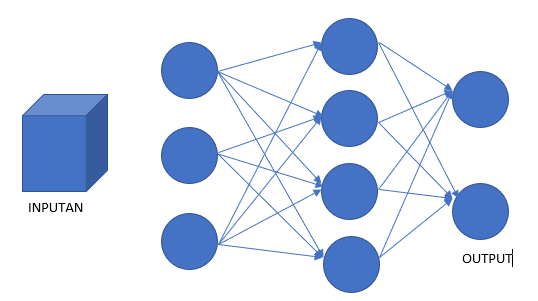
\includegraphics[scale=0.5]{figures/1174070/6/1,2.PNG}
\caption{Ilustrasi Konsep dasar neural network}
\label{contoh}
\end{figure}


\item Jelaskan konsep pembobotan  dalam neural network. dilengkapidengan ilustrasi gambar. \par
pembobotan dalam neural network yaitu digunakan untuk membedakan objek inputan atau variabel inputan untuk AI misalkan apel dan jeruk digunakan untuk variabel inputan maka dibuat pembobotan anatara kedua benda tersebut untuk menentukan output yang pasti dari inputan yang dilakukan.
\begin{figure}[ht]
\centering
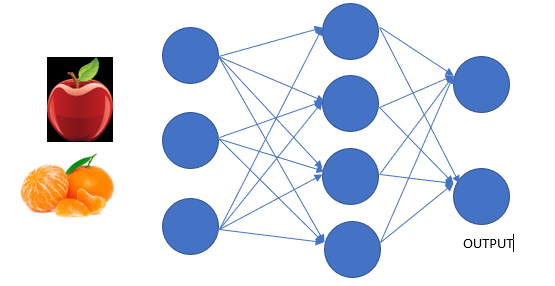
\includegraphics[scale=0.5]{figures/1174070/6/1,3.PNG}
\caption{Ilustrasi Konsep pembobotan pada neural network}
\label{contoh}
\end{figure}

\item Jelaskan konsep aktifitas dalam neural network. dilengkapi dengan ilustrasi gambar.\par
cara aktifitas dalam neural network dilakukan terhadap input pada neural network inputan tersebut dimasukan kepada fungsi pada mesin misalkan fungsi tanh(x) sehingga di hasilkanlah output yang sesuai dengan fungsi tersebut.
\begin{figure}[ht]
\centering
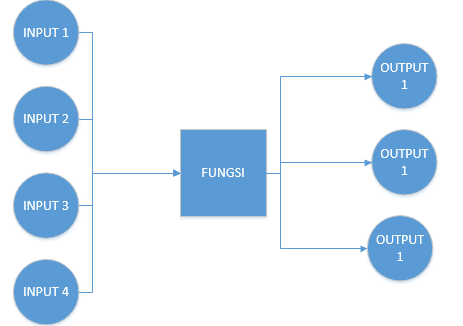
\includegraphics[scale=0.5]{figures/1174070/6/1,4.PNG}
\caption{Gambar yang dibaca hasil plotnya}
\label{contoh}
\end{figure}

\item Jelaskan cara membaca hasil plot dari MFCC dilengkapi dengan ilustrasi gambar. \par
cara membaca hasil ploting dari MFCC yaitu tentukan terlebih dahulu batas minimal Hz dari gelombang suara dan batas maksimal dari suara tersebut. kemudian warna yang paling pekat merupakan hasil dari pengolahan data tersebut misalkan muncul warna orange pekat di bagian bawah dan orange muda di bagian atas yang berarti suara tersebut kuat bagian basnya dan biasanya juga antara warna yang pekat tersebut ada jarak.
\begin{figure}[ht]
\centering
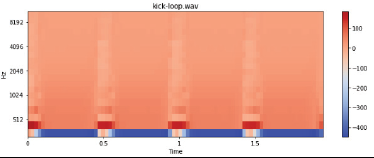
\includegraphics[scale=0.5]{figures/1174070/6/1,5.PNG}
\caption{Ilustrasi Cara Membaca Hasil Plot}
\label{contoh}
\end{figure}

\item Jelaskan apa itu one-hot encoding, dilengkapi dengan ilustrasi kode atau gambar.\par
one-hot encoding merupakan pemberian nilai pada suatu variabel jika nilai itu iya maka nilainya satu dan jika tidak maka nilainya nol.
\begin{figure}[ht]
\centering
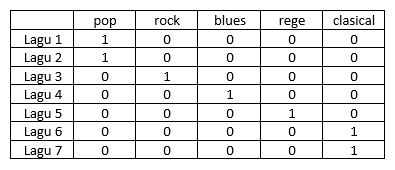
\includegraphics[scale=0.5]{figures/1174070/6/1,6.PNG}
\caption{Ilustrasi Konsep one-hot encoding}
\label{contoh}
\end{figure}

\item Jelaskan apa dari np.unique dan to\_categorical dalam kode program, dilengkapi dengan ilustrasi atau gambar.\par
digunakan untuk membuat array sedangkan  to\_categorical digunakan untuk membuat matrix baui itu 64 bit atau 32 bit.
\begin{figure}[ht]
\centering
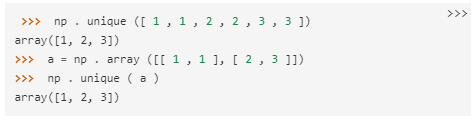
\includegraphics[scale=0.5]{figures/1174070/6/1,7,1.PNG}
\caption{Ilustrasi np.unique}
\label{contoh}
\end{figure}

\begin{figure}[ht]
\centering
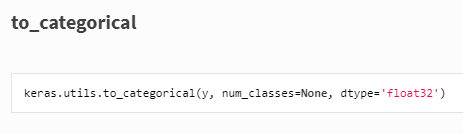
\includegraphics[scale=0.5]{figures/1174070/6/1,7,2.PNG}
\caption{Ilustrasi to\_categorical}
\label{contoh}
\end{figure}


\item Jelaskan apa fungsi dari Sequential dalam kode program, dilengkapi dengan ilustrasi atau gambar. \par
sequential adalah prosesperbandingan setiap elemen satu persatu mulai dari dari objek pertama hingga yang di tuju atau jika mencari angka 100 maka sequential akan membagi bagian misalnya dari satu sampai 20 dan seterusnya sampai mendapat nilai seratus.
\begin{figure}[ht]
\centering
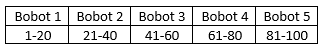
\includegraphics[scale=0.5]{figures/1174070/6/1,8.PNG}
\caption{Ilustrasi Konsep pembobotan pada neural network}
\label{contoh}
\end{figure}

\end{enumerate}

\subsection{Praktikum}
\begin{enumerate}
\item Jelaskan isi dari data GTZAN Genre Collection dan data dari freesound. Buat kode program program untuk meload data tersebut untuk digunakan pada MFCC. Jelaskan arti dari perbaris kode yang dibuat (harus beda dengan teman satukelas).\par
\subitem Isi data data merupakan datasets lagu atau suara yang tersiri dari 10 gendre yang di simpan kedalam 10 folder yaitu folder blues, classical, country, disco, hiphop, jazz, metal, pop, reggae, dan rock ke sepuluh folder tersebut masing-masing  berisi 100 data suara sedangkan data freesound merupakan contoh data suara yang akan di gunakan untuk menguji hasil pengolahan data tersebut dengan menggunakan metode mfcc. apakah suara dari freesound termasuk kategori jazz pop atau sebagainya ?.

\lstinputlisting{src/1174070/6/2,1.py}

\subitem dapat dilihat pada kode diatas pada baris kesatu dilakukan import librosa tang digunakan untuk fungsi mfcc pada suara.
pada baris kedua dilakukan import librosa featuse dan pada baris ke tiga dilakukan librosa display selanjutnya pada baris ke empat dilakukan import glob kemudian insert numpy untuk pengolahan data menjadi vektor setelah itu dilakukan import matplotlib untuk melakukan ploting setelah itu dilakukan import librari keras.\par

\subitem Selanjutnya yaitu membuat fungsi mfcc dengan nama display\_mfcc yang didalamnya terdapat variabel y yang berisi method librosa load kemudian variabel mfcc yang berisi method librosa featurea mfcc. Setelah itu membuat flot figure dengan ukuran 10 banding 4 kemudian di isi oleh data librosa display dengan variabel x nya yaitu waktu dan y yaitu mel atau Hz kemudian melakukan plot warna setelah itu melakukan plot judul dan terakhir flot di tampilkan. 

\item Jelaskan perbaris kode program dengan kata-kata dan di lengkapi ilustrasi gambar fungsi dari display\_mfcc().\par

\lstinputlisting{src/1174070/6/2,2.py}

\subitem pada baris ke dua program diatas digunakan untuk mendisplay tampilan glombang suara dari file 266093\_\_stereo-surgeon\_\_kick-loop-5.wav menggunakan metode mfcc dengan menggunakan fungsi display\_mfcc yang telah tadi di buat pada nomer dua begitu juga pada baris ke 4 6 8 sampai ke 22 secara teksis sama menggunakan fungsi display\_mfcc hanyasaja beda peyimpanan data yang akan di tampilkan atau di eksekusi. untuk contoh hasilnya dapat dilihat pada gambar \ref{c122} berikut:
\begin{figure}[ht]
\centering
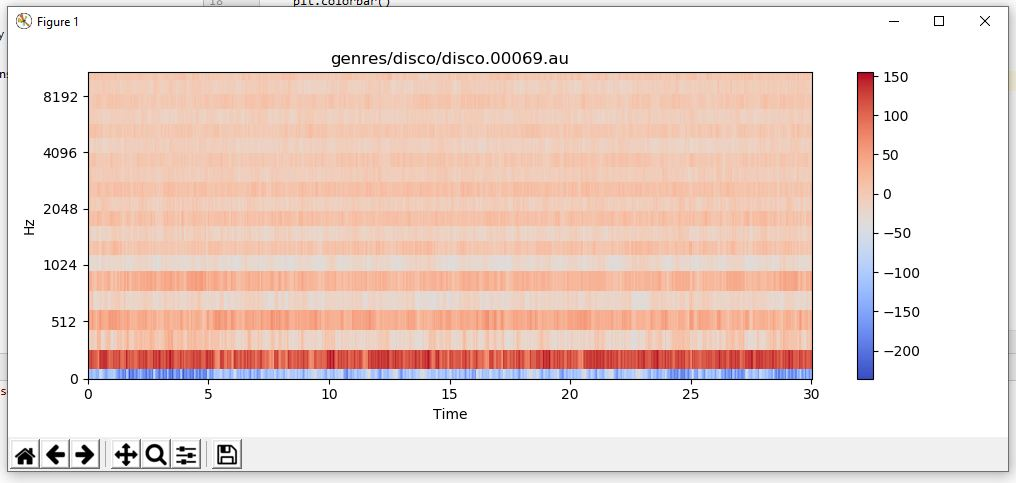
\includegraphics[scale=0.5]{figures/1174070/6/2,2.JPG}
\caption{Ilustrasi gambar fungsi dari display\_mfcc() }
\label{contoh}
\end{figure}

Gambar tersebut merupakan hasil dari mfcc dari salah satu gender lagu pop yang ada pada datasets yang 1000 atau terdapat dalam sepuluh folder tadi.

\item Jelaskan perbaris dengan kata-kata dan dilengkapi dengan ilustrasi gambar fungsi dari extract\_features\_song jelaskan kenapa data yangdiambil merupakan data 25.000 baris pertama ? 

\lstinputlisting{src/1174070/6/2,3.py}

\subitem pada baris ke tiga di definisikan nama extract\_features\_song yang nantinya akan di gunakan pada fungsi yang lainya kemudian dibuat variabel y dengan method librosa load setelah itu dibuat variabel baru mfcc dengan isi librosa features mfcc dengan isi variabel y tadi kemudian dibuat variabel mfcc dengan isian np.max dan variabel mfcc tadi terakhir di buat array dari data tersebut merupakan data 25000 data pertama. kenapa data 25000 pertama yang digunakan dikarenakan data tersebut digunakan sebagai data testing semakin besar data testing yang di gunakan maka semakin akurat hasil AI. tapi sebenarnya data tersebut relatif bisa lebih besar atau lebih kecil tergantung pada komputer masing masing.

\item Jelaskan Perbaris kode program dengan kata-kata dan di lengkapi ilustrasi gambar fungsi dari generate features and labels.

\lstinputlisting{src/1174070/6/2,4.py}

\subitem pada baris ke tiga merupakan pendefinisian nama fungsi yaitu generate features and labels kemudian membuat variabel baru dengan array kosing yaitu all\_features dan all\_labels kemudian mendefinisikan isian label untuk gendre dengan cara membuat variabel genres kemudian di isi dengan 10 gendre yang tadi setelah itu dilakukan fungsi if else dengan code for dan in setelah itu akan di buat encoding untuk data tiap tiap label contoh untuk blues 1000000000 dan untuk clasical 0100000000.

\item Jelaskan dengan kata dan praktek kenapa penggunaan fungsi generate features and labels sangat lama saat meload dataset gendre tunjukan keluarannya dari komputer sendiri dan artikan maksud dari luaran tersebut.\par

halnini menjadi lama dikarenakan mesin membaca satupersatu file yang ada pada folder dan dalam foldertersebut terdapat 100 file sehingga wajar menjadi lama ditambah lagi mengolah data yang tadinya suara menjadi bentuk vektor. berikut merupakan codenya.
\lstinputlisting{src/1174070/6/2,5.py}
\begin{figure}[ht]
\centering
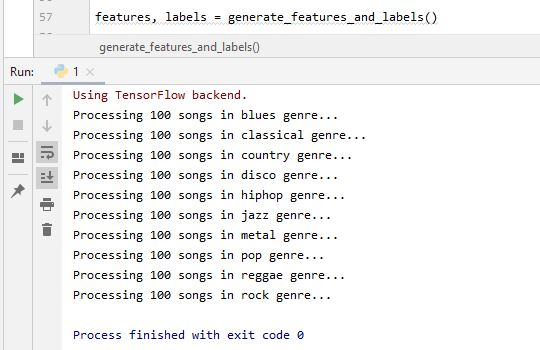
\includegraphics[scale=0.5]{figures/1174070/6/2,5.JPG}
\caption{Hasil dari fungsi generate features and labels}
\label{contoh}
\end{figure}


\item jelaskan kenapa harus dilakukan pemisahan data training dan data testing sebesar 80 persen praktekan dengan kode dan tunjukan keluarannya dari komputer sendiri dan artikan maksud dari luaran tersebut. 
untuk code nya adalah sebagai berikut  yang merupakan code untuk membagi data sebanyak 80 persen untuk data training maka data musik tadi yang total jumlahnya 1000 akan di bagi dua untuk data training sebanyak 800  dan 200 untuk data testing.
\lstinputlisting{src/1174070/6/2,6.py}


\item praktekan dan jelaskan masing masing parameter dari fungsi Sequential().  tunjukan keluarannya dari komputer sendiri dan artikan maksud dari luaran tersebut.\par
\subitem fungsi sequential digunakan untuk mengolah data inputan sesuai dengan fungsi yang ada pada fungsi sequential pada fungsi sequential kali ini menggunakan dua fungsi sequential mengkompile data dari 100 neuron atau dari 1 folder file dengan menggunakan fungsi relu dan softmax untuk menghasilkan outputan yang sesuai dengan keriteria.
\lstinputlisting{src/1174070/6/2,7.py}


\item praktekan dan jelaskan masing masing parameter dari fungsi compile().  tunjukan keluarannya dari komputer sendiri dan artikan maksud dari luaran tersebut. \par
\subitem yaitu fungsi kompile yang digunakan untuk mengetahui parameter yang digunakan dari data yang telah diolah untuk caranya dapat menggunakan codingan sebagai berikut, pada gambar tersebut memunculkan parameternya berapasaja dan total parameter yang digunakan.
\lstinputlisting{src/1174070/6/2,8.py}
\begin{figure}[ht]
\centering
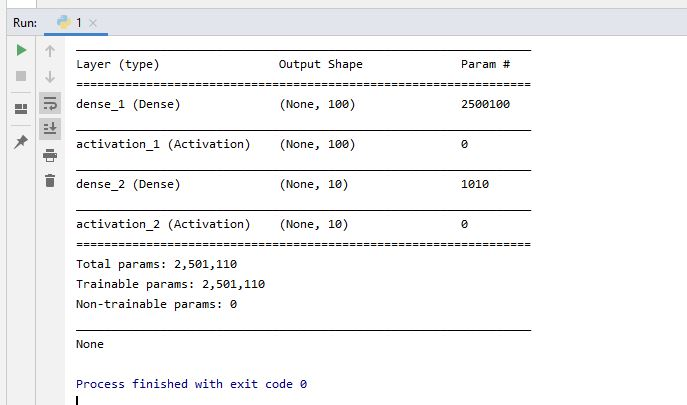
\includegraphics[scale=0.5]{figures/1174070/6/2,8.JPG}
\caption{Hasil fungsi compile}
\label{contoh}
\end{figure}

\item praktekan dan jelaskan masing masing parameter dari fungsi fit().  tunjukan keluarannya dari komputer sendiri dan artikan maksud dari luaran tersebut.\par
\subitem pada fungsi ini dilakukan pengolahan data dari 10 label tadi atau 10 file data sets tadi kemudian di hitung tingkat akurasi masing masing dan tingkat kegagalan atau loss data darisetiap file tersebut caranya dengan melakukan codingan berikut. pada gambar tersebut menunjukan 10 pengolahan data untuk menentukan nilai akurasi dan loss dari data tersebut dan selanjutnya dilakukan fingsi evaluasi.
\lstinputlisting{src/1174070/6/2,9.py}
\begin{figure}[ht]
\centering
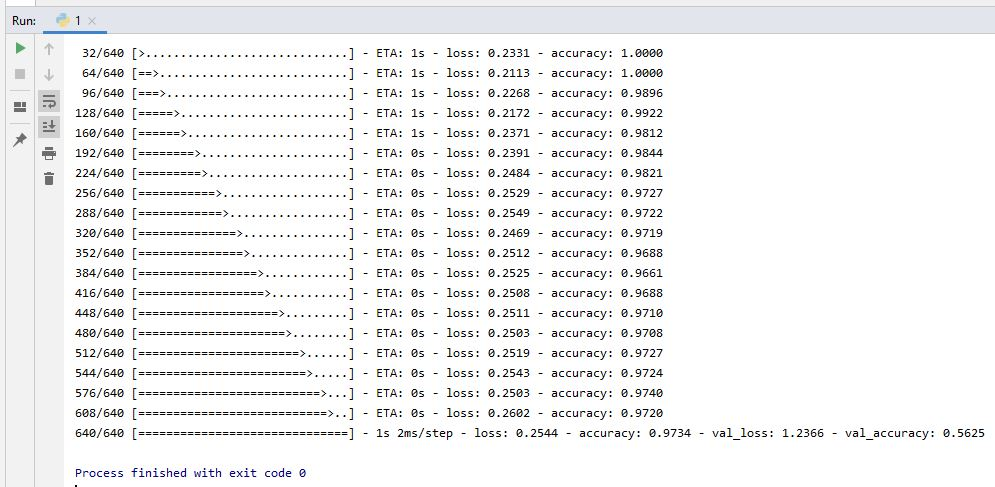
\includegraphics[scale=0.5]{figures/1174070/6/2,9.JPG}
\caption{Hasil fungsi fit}
\label{contoh}
\end{figure}

\item praktekan dan jelaskan masing masing parameter dari fungsi evaluate().  tunjukan keluarannya dari komputer sendiri dan artikan maksud dari luaran tersebut.\par
\subitem pada fungsi ini dilakukan evaluasi terhadap datayang telah di runing sebelummnya untuk lebih jelasnya dapat di lihat codingan tersebut  pada codingan tersebut dilakukan evaluasi pada tingkat kegagalan dan akurasi kebenaran maka hasilnya munculkan hasil evaluasi dari 10 proses dari setiap gendre yaitu akurasi sebesar 51 persen dan loss data sebesar 1.4105 data.
\lstinputlisting{src/1174070/6/2,10.py}
\begin{figure}[ht]
\centering
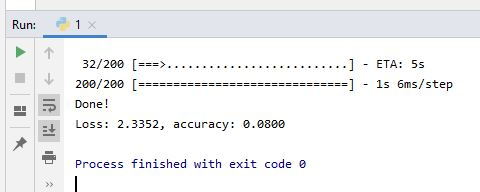
\includegraphics[scale=0.5]{figures/1174070/6/2,10.JPG}
\caption{Hasil fungsi evaluasi}
\label{contoh}
\end{figure}

\item praktekan dan jelaskan masing masing parameter dari fungsi predic  tunjukan keluarannya dari komputer sendiri dan artikan maksud dari luaran tersebut. \par 
\subitem fungsi predic merupakan fungsi untuk membandingkan tingkat akurasi pada setiap label yang sepuluh tadi maka data akan di sandingkan ke masing masing tingkat akurasinya, yang akurasinya paling tinggi maka itulah jawaban untuk setiap inputan yang dilakukan. 
\lstinputlisting{src/1174070/6/2,11.py}
\begin{figure}[ht]
\centering
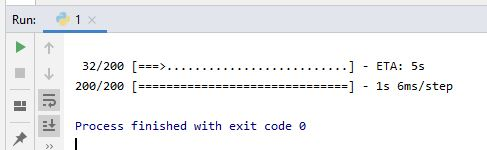
\includegraphics[scale=0.5]{figures/1174070/6/2,11.JPG}
\caption{Hasil fungsi prediksi}
\label{contoh}
\end{figure}

Alhamduluillah
\end{enumerate}


\section{Fanny Shafira Damayanti (1174069)}
\subsection{Teori}
\begin{enumerate}
\item Definisi Kecerdasan buatan\\ 
Kecerdasan buatan atau Artificial intelligence merupakan kecerdasan yang ditambahkkan kedalam suatu system yang diatur secara ilmiah. Kecerdasan buatan dibuat untuk menggantikan pekerjaan yang dilakukan oleh manusia menjadi dikerjakan oleh sistem.

\item Sejarah Kecerdasan Buatan
\begin{itemize}
\item Abad 17, Rene Descartes berkata bahwa tubuh hewan adalah sekumpulan mesin yang rumit.
\item 1642, Blaise Pascal menciptakan mesin penghitung digital mekanis pertama.
\item Abad 19, Charles Babbage dan Ada Lovelace bekerja di program penghitung mekanis.
\item 1950, John McCarthy membuat istilah “Kecerdasan Buatan”.
\item 1960-1970, Joel Moses membuat program yang pertama kali sukses dalam bidang matematika.
\item 1980, jaringan saraf digunakan secara meluas dengan algoritme perambatan balik.
\item 2004, DARPA membuat kendaraan yang bisa dijalankan sendiri tanpa manusia.
\end{itemize}

\item Perkembangan kecerdasan buatan
\begin{itemize}
\item Masa persiapan (1943-1946)
Warren McCulloch dan Walter Pitt mengemukakan tiga hal : pengetahuan fisiologi dasar dan fungsi sel syaraf dalam otak, analisa formal tentang logika proposisi, dan teori komputasi Turing.

Pada tahun 1950, Nobert Wiener membuat penelitian mengenai prinsip-prinsip teori feedback.

Pada tahun 1956, John McCarthy meyakinkan Minsky, Claude Shannon dan Nathaniel Rochester untuk membantunya melakukan penelitian dalam bidan Otomata, Jaringan Syaraf dan pembelajaran intelijensia. 

\item Awal perkembangan (1952-1969)
Pada tahun 1958, McCarthy di MIT AI Lab Memo No.1 mendefinisikan bahasa pemrograman tingkat tinggi yaitu LISP,

Pada tahun 1959, Nathaniel Rochester dari IBM dan mahasiswa-mahasiswanya mengeluarkan program kecerdasan buatan yaitu Geometry Theorm Prover.

Pada tahun 1963, program yang dibuat James Slagle mampu menyelesaikan masalah integral tertutup untuk mata kuliah Kalkulus.
Pada tahun 1986, program analogi buatan Tom Evan menyelesaikan masalah analogi geometris yang ada pada tes IQ.

\item Perkembangan Kecerdasan Buatan Melambat (1969-1979)
Bruce Buchanan dan Joshua Lederberg yang membuat program untuk memecahkan masalah struktur molekul dari informasi yang didapatkan dari spectrometer massa.

\item AI Menjadi sebuah industri
Industrialisasi kecerdasan buatan diawali dengan ditemukannya sistem pakar yang dinamakan R1 yang mampu mengkonfigurasi system-sistem computer baru. 

\item Kembalinya Jaringan Syaraf Tiruan (1986-sekarang)
Pada tahun 1985-an setidaknya empat kelompok riset menemukan kembali algoritma belajar propagasi balik (Black-Propagation Learning). Algoritma ini berhasil diimplementasikan ke dalam bidang ilmu computer dan psikologi.
\end{itemize}

\item Definisi Supervised Learning\\
Supervised Learning merupakan cabang dari Artificial Intelligence. supervised learning adalah suatu ilmu yang mempelajari perancangan dan pengembangan algoritma.

\item Klasifikasi Supervised Learning
\begin{itemize}
\item Logistic regression.
\item K-nearest neighbors.
\item Support vector machine (SVM)
\item Naive Bayes.
\item Decision tree classification.
\item Random forest classification.
\end{itemize}

\item Regresi dan Unsupervised Learning\\
Regresi merupakan sebuah metode analisis statistic yang digunkan untuk mengetahui pengaruh antara dua variable atau lebih.

Untuk mempelajari Unsupervised learning kita tidak perlu data training untuk melakukan prediksi maupun klasifikasi.

\item Dataset\\
Dataset merupakan objek yang mempresentasikan data dan relasinya pada memori.

\item Training Set\\
Training Set merupakan bagian dari dataset untuk membuat prediksi atau menjalankan fungsi dari sebuah algoritma Machine Learning.

\item Testing Set\\
Testing set digunakan untuk mengukur apakah classifier berhasil melakukan klasifikasi dengan benar.

\end{enumerate}

\subsection{Instalasi}
\begin{enumerate}
	\item Instalasi Library scikit dari anaconda, mencoba kompilasi dan uji coba ambil contoh kode dan lihat variabel explorer
	\hfill\break
	\begin{figure}[H]
		\includegraphics[width=4cm]{figures/1174069/1/1.PNG}
		\centering
		\caption{Instalasi Package Scikit Learn}
	\end{figure}
	\begin{figure}[H]
		\includegraphics[width=4cm]{figures/1174069/1/2.png}
		\centering
		\caption{Isi Variabel Explorer}
	\end{figure}
	\item Mencoba Loading an example dataset, menjelaskan maksud dari tulisan tersebut dan mengartikan           		  per baris
	\hfill\break
	\lstinputlisting[firstline=7, lastline=11]{src/1174069/1/1174069.py}
	\item Mencoba Learning and predicting, menjelaskan maksud dari tulisan tersebut dan mengartikan per  			  baris
	\hfill\break
	\lstinputlisting[firstline=13, lastline=22]{src/1174069/1/1174069.py}
	\item  Mencoba Model persistence, menjelaskan maksud dari tulisan tersebut dan mengartikan per baris
	\hfill\break
	\lstinputlisting[firstline=25, lastline=34]{src/1174069/1/1174069.py}
	\item Mencoba Conventions, menjelaskan maksud dari tulisan tersebut dan mengartikan per baris
	\hfill\break
	\lstinputlisting[firstline=37, lastline=48]{src/1174069/1/1174069.py}
\end{enumerate}

\subsection{Penanganan Error}
\begin{enumerate}
	\item ScreenShoot Error
	\begin{figure}[H]
		\includegraphics[width=4cm]{figures/1174069/1/error/1.png}
		\centering
		\caption{Import Error}
	\end{figure}

	\item Tuliskan Kode Error dan Jenis Error
	\begin{itemize}
		\item Import Error
	\end{itemize}
	\item Cara Penangan Error
	\begin{itemize}
		\item Import Error
		\hfill\break
		Dengan Menginstall Library Yang Tidak Ditemukan
	\end{itemize}
\end{enumerate}

\subsection{Bukti Tidak Plagiat}
\begin{figure}[H]
	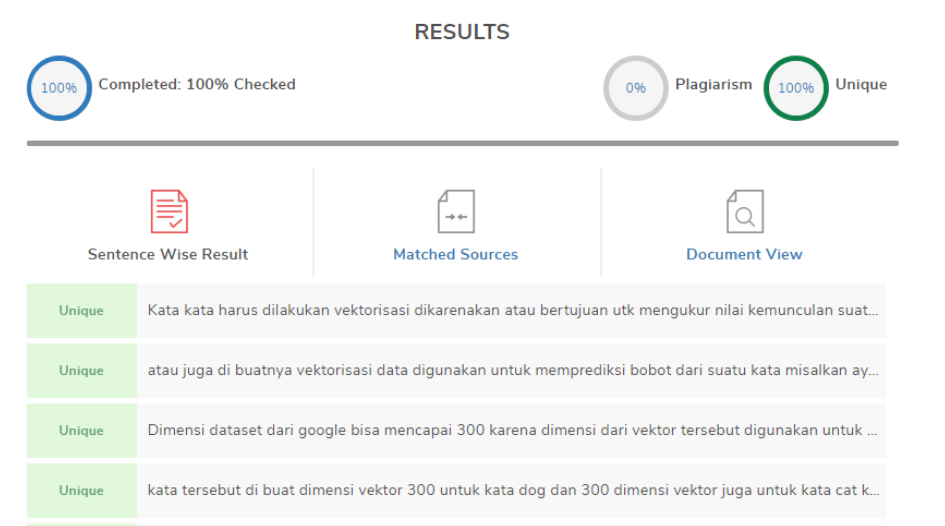
\includegraphics[width=4cm]{figures/1174069/1/plagiat/plagiat.PNG}
	\centering
	\caption{Bukti Tidak Melakukan Plagiat Chapter 1}
\end{figure}

\subsection{Link Youtube}
https://youtu.be/Ra4Lu-C8OQY

\section{Tia Nur Candida - 1174086}
\subsection{Teori}
\begin{enumerate}
\item Definisi Kecerdasan Buatan \\
Kecerdasan Buatan adalah suatu ilmu yang mempelajari bagaimana cara komputer melakukan sesuatu seperti yang dilakukan oleh manusia. Secara sederhana AI adalah teknik dan ilmu untuk membangun atau membuat suatu mesin menjadi cerdas, terutama pada program komputer. Kecerdasan yang dimaksud yaitu seperti yang dimiliki oleh manusia namun pada mesin akan dibuat cepat dan tepat atau akurat.

\item Sejarah Kecerdasan Buatan \\
Sejarah kecerdasan buatan dimulai pada zaman kuno. Benih kecerdasan buatan modern ditanamkan oleh filusuf klasik dengan berusaha menggambarkan proses berpikir manusia. Karya tersebut memuncak pada penemuan komputer digital yang di program pada tahun 1940 an, dimana terdapat sebuah mesin yang didasarkan pada esensi abstrak penalaran matematika. 
Istilah kecerdasan buatan pertama kali dikemukaan pada tahun 1956 di Konferensi Darthmouth yang kemudian sejak saat itu kecerdasan buatan terus berkembang.

\begin{itemize}
\item Masa Persiapan AI (1943-1956)\\
Pada tahun 1943, Warren McCulloch dan Walter Pitt mengemukakan tiga hal : pengetahuan fisiologi dasar dan fungsi sel syaraf dalam otak, analisa formal tentang logika proposisi, dan teori komputasi Turing. Mereka berhasil membuat suatu model sel syaraf tiruan dimana setiap sel syaraf digambarkan sebagai ‘on’ dan ‘off’. Mereka menunjukkan bahwa setiap fungsi dapat dihitung dengan suatu jaringan sel syaraf dan bahwa semua hubungan logis dapat diimplementasikan dengan struktur jaringan yang sederhana.
Pada tahun 1950, Nobert Wiener membuat penelitian mengenai prinsip-prinsip teori feedback. Contoh yang terkenal adalah thermostat. Penemuan ini juga merupakan awal dari perkembangan AI.

Pada tahun 1956, John McCarthy meyakinkan Minsky, Claude Shannon dan Nathaniel Rochester untuk membantunya melakukan penelitian dalam bidan Otomata, Jaringan Syaraf dan pembelajaran intelijensia. Mereka mengerjakan proyek ini selama 2 bulan di Dartsmouth. Hasilnya adalah program yang mampu berpikir non-numerik dan menyelesaikan masalah pemikiran, yang dinamakan Principia Mathematica. Hal ini menjadikan McCarthy disebut sebagai bapak kecerdasan buatan.


\item Awal perkembangan AI (1952-1969)\\
Kecerdasan buatan banyak mengalami kesuksesan pada tahun pertama. 
Pada tahun 1958, McCarthy di MIT AI Lab Memo No.1 mendefinisikan bahasa pemrograman tingkat tinggi yaiyu LISP, yang sekarang mendominasi pembuatan program-pogram kecerdasan buatan. Kemudian, McCarthy membuat program yang dinamakan Programs with Common Sense. Di dalam program tersebut, dibuat rancangan untuk menggunakan pengetahuan dalam mencari solusi.
Pada tahun 1959, Nathaniel Rochester dari IBM dan mahasiswa-mahasiswanya mengeluarkan program kecerdasan buatan yaitu Geometry Theorm Prover. Program ini dapat mengeluarkan suatu teorema menggunakan aksioma-aksioma yang ada.
Pada tahun 1963, program yang dibuat James Slagle mampu menyelesaikan masalah integral tertutup untuk mata kuliah Kalkulus.
Pada tahun 1986, program analogi buatan Tom Evan menyelesaikan masalah analogi geometris yang ada pada tes IQ.

\item Perkembangan kecerdasan buatan melambat (1966-1974)
Banyak masalah yang perlu di selesaikan oleh kecerdasan buatan dan baru sedikit program yang keluar menyebabkan melambat.

\item Kecerdasan buatan menjadi sebuah industri ( 1980 - 1988 )\\
Industrialisasi kecerdasan buatan diawali dengan ditemukannya sistem pakar yang dinamakan R1 yang mampu mengkonfigurasi system-sistem computer baru. Program tersebut mulai dioperasikan di Digital Equipment Corporation (DEC), McDermott, pada tahun 1982.
Pada tahun 1986, R1 telah berhasil menghemat US Dolar 40 juta per tahun.
Pada tahun 1988, kelompok kecerdasan buatan di DEC menjalankan 40 sistem pakar. Hampir semua perusahaan besar di USA mempunyai divisi AI. Sehingga perusahaan yang sejak tahun 1982 hanya menghasilkan beberapa juta US dolar per tahun meningkat menjadi 2 milyar US dolar per tahun pada tahun 1988.

\item Kembalinya Jaringan Syaraf Tiruan ( 1986 - Sekarang )\\
Meskipun bidang ilmu computer menolak jaringan syaraf tiruan setelah diterbitkannya buku “Perceptrons” karangan Minsky dan Papert, tetapi para ilmuwan masih mempelajari bidang ilmu tersebut dari sudut pandang yang lain yaitu fisika. Para ahli fisika seperti Hopfield (1982) menggunakan teknik-teknik mekanika statistika untuk menganalisa sifat-sifat pentimpanan dan optimasi pada jaringan syaraf. Para ahli psikologi, David Rumelhart dan Geoff Hinton, melanjutkan penelitian mengenai model jaringan syaraf tiruan pada memori.
Pada tahun 1985-an setidaknya empat kelompok riset menemukan kembali algoritma belajar propagasi balik (Black-Propagation Learning). Algoritma ini berhasil diimplementasikan ke dalam bidang ilmu computer dan psikologi.

\end{itemize}
\item Definisi Supervised Learning \\
Merupakan tipe Machine Learning dimana model ini menyediakan training data berlabel. Supervised learning merupakan suatu pembelajaran yang terawasi dimana jika output yang diharapkan telah diketahui sebelumnya.  Supervised Learning adalah tipe learning di mana kita mempunyai variable input dan variable output, dan menggunakan satu algoritma atau lebih untuk mempelajari fungsi pemetaan dari input ke output. Goal-nya adalah untuk memperkirakan fungsi pemetaannya, sehingga ketika kita mempunya input baru, kita dapat memprediksi output untuk input tersebut.

\item Klasifikasi
\begin{itemize}
\item Logistic regression
\item K-nearest neighbors
\item Support vector machine (SVM)
\item Naive Bayes
\item Decision tree classification
\item Random forest classification
\end{itemize}

\item Regresi \\
Regresi adalah suatu metode analisis statistik yang digunakan untuk melihat pengaruh antara dua atau lebih banyak variabel. Hubungan variabel tersebut bersifat fungsional yang diwujudkan dalam suatu model matematis.

\item Unsupervised Learning \\
Unsupervised Learning adalah tipe learning di mana kita hanya mempunyai data masukan (input data) tetapi tidak ada output variable yang berhubungan.\\
Goal dari unsupervised learning adalah untuk memodelkan struktur dasar atau distribusi dalam data dengan tujuan untuk mempelajari data lebih jauh lagi, dengan kata lain, adalah menyimpulkan fungsi yang mendeskripsikan atau menjelaskan data.

\item Dataset \\
Dataset adalah objek yang merepresentasikan data dan relasinya di memory. Strukturnya mirip dengan data di database. Dataset berisi koleksi dari datatable dan datarelation.
\item Training Set \\
Training set adalah bagian dataset yang kita latih untuk membuat prediksi atau menjalankan fungsi dari sebuah algoritma ML lainnya sesuai tujuannya masing-masing. Kita memberikan petunjuk melalui algoritma agar mesin yang kita latih bisa mencari korelasinya sendiri.
\item Test Set \\
Test set adalah bagian dataset yang kita tes untuk melihat keakuratannya, atau dengan kata lain melihat performanya.

\end{enumerate}
\subsection{Praktek}
\begin{enumerate}
	\item Instalasi Library scikit dari anaconda, mencoba kompilasi dan uji coba ambil contoh kode dan lihat variabel explorer
	\hfill\break
	\begin{figure}[H]
		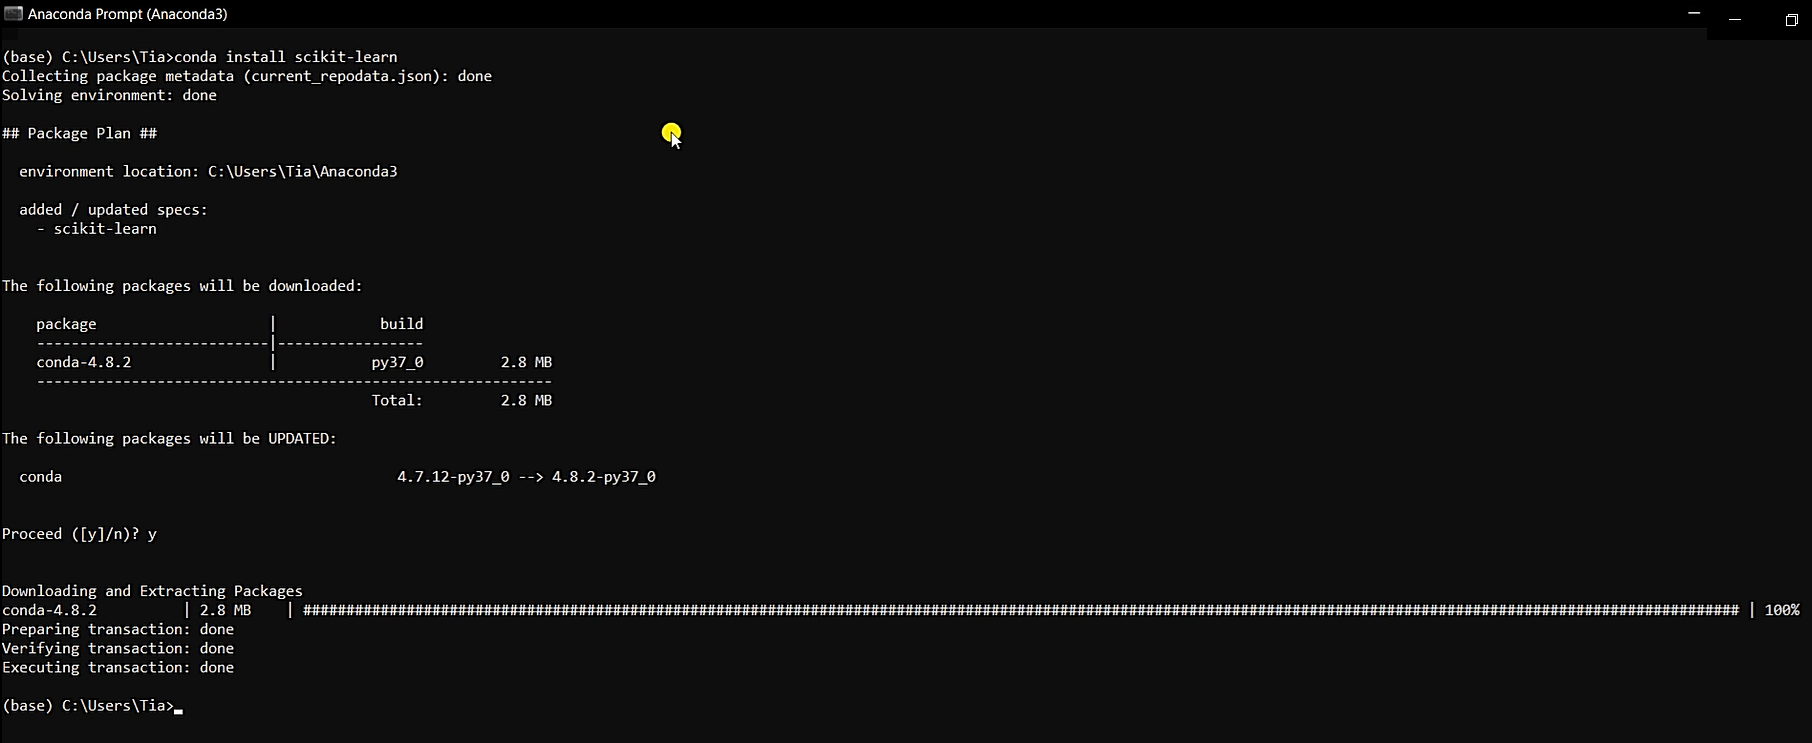
\includegraphics[width=4cm]{figures/1174086/1/installasi.PNG}
		\centering
		\caption{Instalasi Package Scikit Learn}
	\end{figure}
	\begin{figure}[H]
		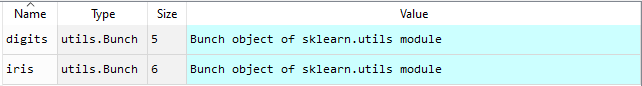
\includegraphics[width=4cm]{figures/1174086/1/variabel.png}
		\centering
		\caption{Isi Variabel Explorer}
	\end{figure}
	\item Mencoba loading an example dataset
	\hfill\break
	\lstinputlisting[firstline=7, lastline=11]{src/1174086/1/1174086.py}
	\item Mencoba Learning dan predicting
	\hfill\break
	\lstinputlisting[firstline=13, lastline=22]{src/1174086/1/1174086.py}
	\item Mencoba Model Persistence
	\hfill\break
	\lstinputlisting[firstline=25, lastline=34]{src/1174086/1/1174086.py}
	\item Mencoba Conventions
	\hfill\break
	\lstinputlisting[firstline=37, lastline=48]{src/1174086/1/1174086.py}
\end{enumerate}

\subsection{Bukti Tidak Plagiat}
\begin{figure}[H]
	\includegraphics[width=4cm]{figures/1174086/bukti/1.png}
	\centering
	\caption{Bukti Tidak Melakukan Plagiat Chapter 1}
\end{figure}


\section{1174054 | Aulyardha Anindita}

\subsection{Teori}
\begin{enumerate}
\item Definisi, Sejarah dan Perkembangan Kecerdasan Buatan
\begin{itemize}
\item Definisi Kecerdasan Buatan\\
Kecerdasan buatan adalah suatu kecerdasan yang didalamnya berisi suatu system yang biasa diatur dalam sebuah konteks ilmiah. Kecerdasan  buatan juga bisa didefinisikan sebagai sebuah kecerdasan yang diciptakan dan dimasukkan kedalam suatu mesin computer agar dapat melakukan pekerjaan seperti yang dapat dilakukan oleh manusia. Ada beberapa macam bidang atau ilmu yang menggunakan kecerdasan buatan diantaranya adalah system pakar, permainan computer (game), logika fuzzy, jaringan saraf tiruan dan robotika.\\
Penelitian dalam AI mencakup pembuatan mesin dan suatu program computer untuk mengotomatisasikan tugas-tugas yang membutuhkan perilaku cerdas, seperti : pengendalian, perencanaan dan penjadwalan serta kemampuan untuk menjawab diagnose dan pertanyaan pelanggan serta pengenalan tulisan tangan. Suara dan wajah

\item Sejarah Kecerdasan Buatan
\begin{itemize}
\item Pada tahun 1940 dan 1950 Artificial Inteligence merupakan suatu inovasi baru dalam bidang ilmu pengetahuan dimana pada tahun ini computer modern sudah ada
\item Pada tahun 1950 awal, studi tentang “mesin berfikir” mempunyai berbegai nama seperti cybernetics, teori automata, dan pemrosesan informasi
\item Pada tahun 1956, para ilmuwan jenius seperti Alan Turing, Norbert, Wiener, Claude Shannon dan Warren McCullough bekerja secara independen di bidang cybernetics, matematika, algoritma dan teori jaringan. John McCarthy merupakan orang yang menciptakan istilah tersebut dan mendirikan laboratorium kecerdasan buatan di MIT dan Stanford
\item Pada tahun 1956, McCarthy mendirikan Konferensi Dartmouth di Hanover, New Hampshire. Dia merupakan peneliti terkemuka dalam teori kompleksitas, simulasi Bahasa, dan hubungan antara keacakan dan pemikiran kreatif, jaringan saraf diundang. Sehingga Konferensi Dartmouth 1956 dianggap sebagai kelahiran Kecerdasan Buatan.
\item Sejak saat itu, Kecerdasan Buatan telah hidup melalui decade kemuliaan dan cemohan yang dikenal dengan luas sebagai musim panas dan musim dingin Ai.
\end{itemize}

\item Perkembangan Kecerdasan Buatan\\
Saat ini, teknologi Artificial Intelligence sangat ramai diperbincangkan oleh masyarakat. Sudah banyak pekerjaan yang hilang karena adanya AI, seperti pekerjaan kasir, penjaga pintu tol, parkir, dan sebagainya. Hal ini terjadi karena AI lebih unggul dalam hal kinerja, fitur dan lain sebagainya. Walaupun masih ada beberapa aspek yang memang pekerja manusia masih unggul dibandingkan AI itu sendiri. \\
Berdasarkan survei yang dilakukan oleh Microsoft, hasilnya adalah 39 responden masih mempertimbangkan untuk menggunakan mobil tanpa pengemudi dan sebanyak 36 responden lainnya setuju mahwa robot atau AI dengan menggunakan software untuk beroperasi mampu meningkatan produktivitas. Dari survei tersebut, dapat ditarik kesimpulan bahwa pengguna AI harus lebih bijaksana dalam pengembangan dan penggunaan dari AI sehingga tidak memiliki efek samping terhadap profuktifitas kerja dan keseharian sebagai pengguna dalam kehidupan sehari-hari.

\end{itemize}

\item Definisi Supervised Learning, Klasifikasi, Regresi, Unsupervised Learning, Data Set, Training Set dan Testing Set
\begin{itemize}
\item Supervised Learning\\
Supervised learning adalah suatu tugas pengumpulan data yang berfungsi untum menyimpulkan fungsi dari data pelatihan yang berlabel. Didalam Supervised Learning, setiap contoh merupakan pasangan yang terdiri dari objek input dan nilai output yang diinginkan. Algoritma pembelajaran yang diawasi berupa menganalisis data pelatihan dan menghasilkan fungsi yang disimpulkan yang digunakan untuk memetakan contoh baru.\\
 	Supervised Learning adalah suatu pendekatan dimana sudah terdapat data yang dilatih selain itu juga sudah memiliki variable yang ditargetkan sehingga tujuan dari pendekatan tersebut adalah mengelompokkan suatu data ke data yang sudah ada. Supervised learning sendiri menyediakan algoritma pembelajaran dengan jumlah yang diketahui untuk mendukung penilaian dimasa depan. Supervised learning sebagian besar memiliki kaitan dengan AI dengan menggunakan model pembelajaran generatif. Data pelatihan untuk pembelajaran yang diawasi mencakup beberapa contoh dengan subjek input yang berpasangan dan output yang diinginkan.\\
 	Modul supervised learning mempunyai beberapa keunggulan dibandingkan pendekatan tanpa pengawasan, tapi mereka juga memiliki keterbatasan. System lebih cenderung membuat penilaian bahwa manusia dapat berhubungan, misalnya manusia mempunyai dasar untuk keputusan. Tapi, dalam kasus tersebut yang menggunakan metode berbasis pengambilan, supervised learning mengalami kseulitan dalam menangani suatu informasi baru. 

\item Klasifikasi\\
Klasifikasi merupakan pembagian menurut kelas-kelas. Menurut ilmu pengetahuan, klasifikasi adalah suatu proses pengelompokkan benda berdasarkan ciri-ciri persamaan dan perbedaan. Dalam pembelajaran mesin dan statistic, klasifikasi merupakan suatu pendekatan pembelajaran yang diawasi dimana program computer tersebut belajar dari input data yang diberkan kepadanya lalu menggunakan pembelajaran tersebut untuk mengklasifikasikan pengamatan baru. Kumpulan data tersebut mungkin hanya bersifat dua kelas atau mungkin juga multi-kelas.

\item Regresi\\
Regresi adalah suatu metode analisis statistik yang digunakan untuk melihat pengaruh antara dua atau lebih variable. Regresi sendiri membahas masalah ketika variable output yaitu nilai ril atau berkelanjutan seperti gaji atau berat. Banyak model yang dapat digunakan, yang paling sederhana adalah regresi linear.

\item Unsupervised Learning\\
Unsupervised learning berbeda dengan supervised learning, perbedaanya yaitu unsupervised learning tidak memiliki data pelatihan, sehingga data dapat dikelompokkan menjadi dua atau 3 begitupun seterusnya. Unsupervised learning adalah suatu pelatihan algoritma kecerdasan buatan (AI) menggunakan beberapa informasi yang tidak diklasifikasikan atau diberi label dan memungkinkan algoritma  untuk bertindak atas informasi tersebut. System AI disini dapat dikelompokkan berdasarkan informasi yang tidak disortir berdasarkan persamaan dan perbedaan meskipun tidak ada kategori yang disediakan. System AI disajikan dengan data yang tidak berlabel, tidak terkategorisasi dan algoritma system bekerja pada data tanpa pelatihan sebelumnya sehingga outputmya tergantung pada algoritma kode.

\item Data Set\\
Data set adalah suatu objek yang merepresentasikan data dan memiliki relasi yang ada di dalam memory. Struktur data set mirip dengan data yang ada didatabase, namun bedanya data set berisi koleksi dari data table dan data relation. Untuk mendapatkan data yang tepat, berarti mengumpulkan atau mengidentifikasi data yang berkorelasi dengan hasil yang ingin anda prediksi.

\item Training Set\\
Training set adalah salah satu set yang biasa digunakan oleh algoritma klasifikasi. Seperti decision tree, bayesian, neural network, dll. Mereka dapat digunakan untuk membentuk model classifier, dalam menjalankan pelatihan yang diatur melalui jaringan saraf yang mengajarkan pada net dengan cara menimbang berbagai fitur, menyesuaikan koefisien berdasarkan kemungkinan mereka meminimalkan kesalahan. Kofiesen tersebut juga dikenal sebagai parameter.

\item Testing Set\\
Testing set adalah salah satu set yang digunakan untuk mengukur sejauh mana classifier berhasil melakukan klasifikasi dengan benar. Hal ini berfungsi sebagai materai persetujuan tapi tak digunakan sampai akhir. Setelah melatih dan mengoptimalkan data, kita dapat melakukan pengujian sarat terhadap pengambilan sampel aca. Dan hasilnya harus memvalidasi bahwa jaring data tersebut secara akurat mengenali gambar atau mengenali setidaknya (x) dari jumlah tersebut.

\end{itemize}
\end{enumerate}

\subsection{Praktek}
\begin{enumerate}
\item Instalasi library scikit dari anaconda
\hfill\break
	\begin{figure}[H]
		\includegraphics[width=4cm]{figures/1174054/1/1.png}
		\centering
		\caption{Instalasi Package Scikit Learn}
	\end{figure}
	\begin{figure}[H]
		\includegraphics[width=4cm]{figures/1174054/1/2.png}
		\centering
		\caption{Isi Variabel Explorer}
	\end{figure}
\item Mencoba Loading an example dataset
\hfill\break
	\lstinputlisting[firstline=8, lastline=12]{src/1174054/1/1174054.py}
	
\item Mencoba Learning and predicting
\hfill\break
	\lstinputlisting[firstline=14, lastline=24]{src/1174054/1/1174054.py}
	
\item Mencoba Model persistence
\hfill\break
	\lstinputlisting[firstline=26, lastline=36]{src/1174054/1/1174054.py}
	
\item Mencoba Conventions
\hfill\break
	\lstinputlisting[firstline=38, lastline=50]{src/1174054/1/1174054.py}
\end{enumerate}

\subsection{Penanganan Error}
\begin{enumerate}
\item ScreenShoot Error
	\begin{figure}[H]
		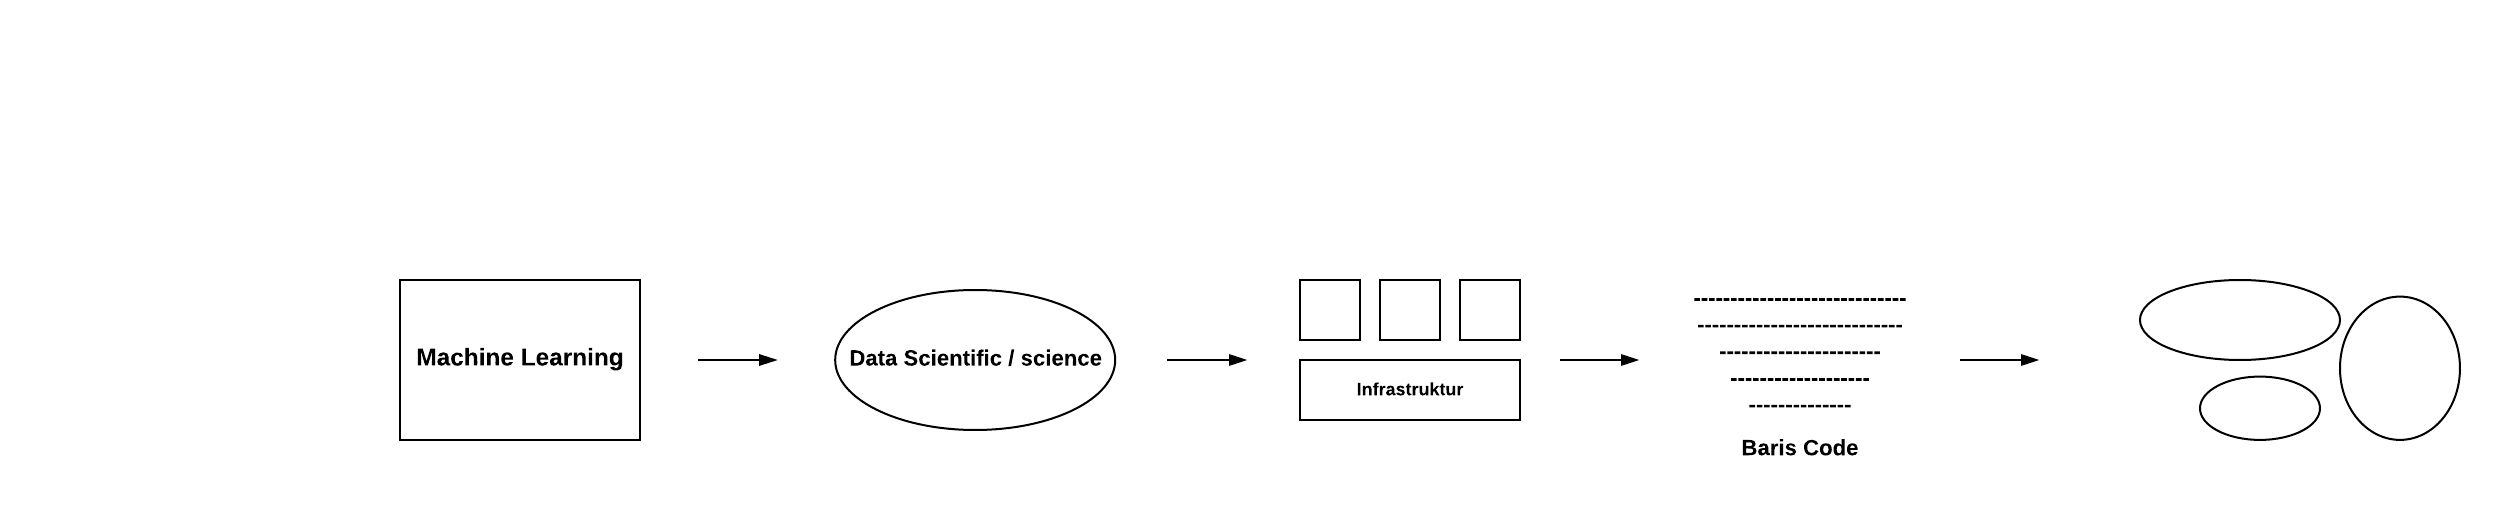
\includegraphics[width=4cm]{figures/1174054/1/3.png}
		\centering
		\caption{Module Not Found Error}
	\end{figure}
	\begin{figure}[H]
		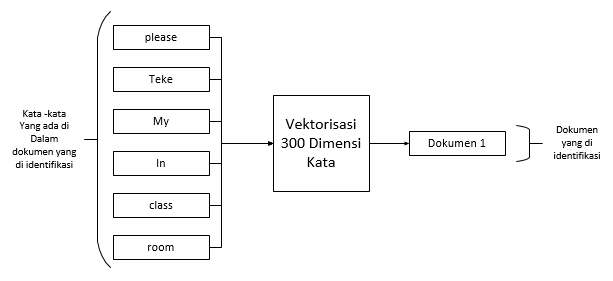
\includegraphics[width=4cm]{figures/1174054/1/4.png}
		\centering
		\caption{Import Error}
	\end{figure}

	\item Tuliskan Kode Error dan Jenis Error
	\begin{itemize}
		\item Module Not Found Error
		\item Import Error
	\end{itemize}
	\item Cara Penanganan Error
	\begin{itemize}
		\item Module Not Found Error
		\hfill\break
		Dengan memperbaiki penulisan atau kesalahan dalam penulisan kode atau melakukan install package atau modul yang belum terinstal
		\item Import Error
		\hfill\break
		Dengan Menginstall Library Yang Tidak Ditemukan
	\end{itemize}
\end{enumerate}


\subsection{Bukti Tidak Plagiat}
\begin{figure}[H]
	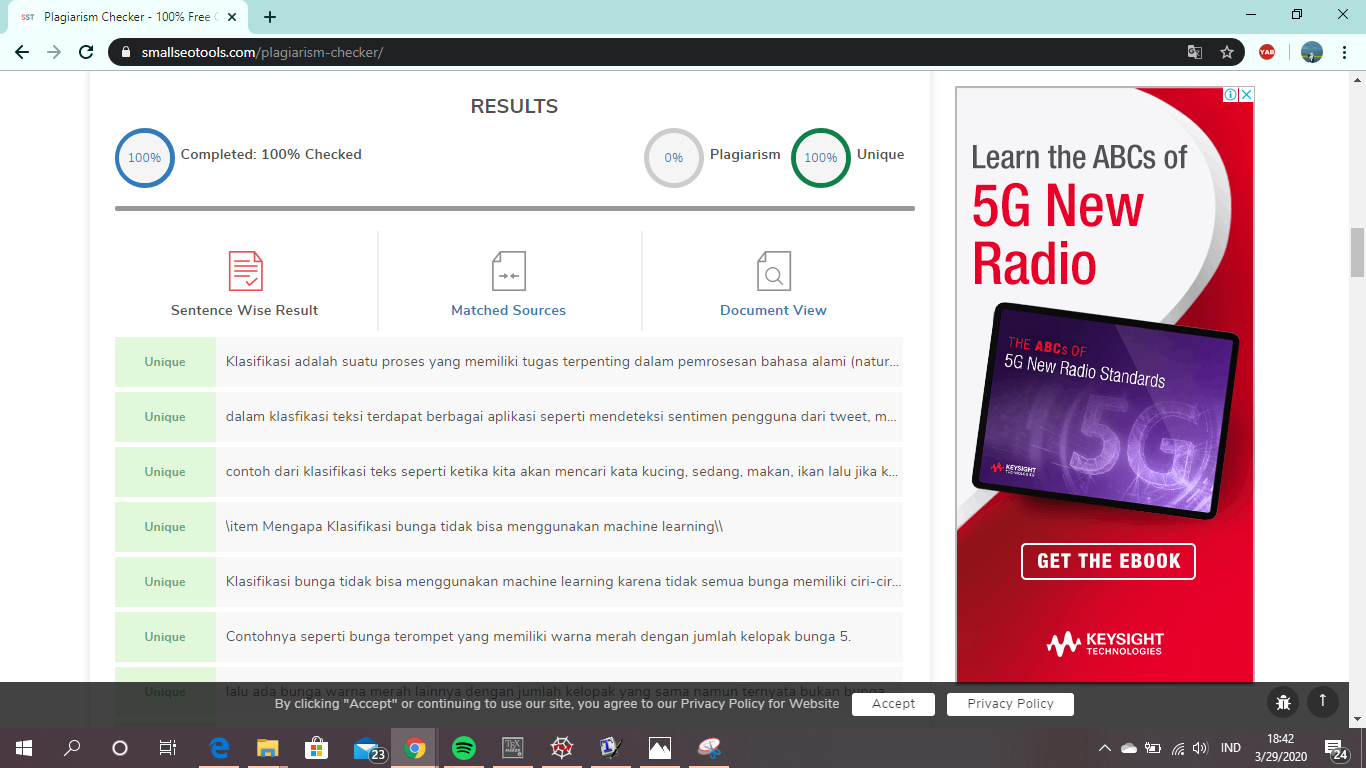
\includegraphics[width=4cm]{figures/1174054/1/plagiarisme.png}
	\centering
	\caption{Bukti Plagiasrisme}
\end{figure}

\subsection{Link Youtube}
https://youtu.be/gl9Q60DzEfI
\section{Ainul Filiani 1174073}
\subsection{Pengertian Kecerdasan Buatan}
kecerdasan buatan adalah salah satu cabang ilmu pengetahuan yang berhubungan dengan mesin untuk memecahkan persoalan yang rumit dengan cara yang lebih manusiawi. Hal ini biasanya dilakukan dengan mengikuti karakteristik dan anologi berpikir dari kecerdasan  atau inteligance manusia, dan menerapkan sebagai algoritma yang dikenal oleh komputer.
Dengan suatu pendekatan yang kurang lebih fleksibilitas dan efisien dapat diambil tergantung keperluan yang mempengaruhi bagaimana wujud dari prilaku kecerdasan buatan. AI biasanya dihubungkan dengan ilmu komputer, akan tetapi juga terkait erat dengan bidang lain seperti matematika, Psikologi, Pengamatan, Biolog, filosofi, dan lainnya
\subsection{Sejarah Kecerdasan Buatan}
Kecerdasan buatan merupakan bidang ilmu komputer yang sangat penting di era kini dan masa yang akan datang untuk mewujudkan sistem komputer yang cerdas. Bidang ini telah berkembang sangat pesat di 20 tahun terakir seiring dengan kebutuhan perangkat cerdas pada industry dan rumah tangga.
Kata Intelligance berasal dari bahasa latin "intelligo" yang berarti "saya paham". Berarti dasar dari intelligance adalah kemampuan untuk memahami dan melakukan aksi. nyatanya, bidang Kecerdasan Buatan atau disingkat dengan AI, berawal dari kemunculan komputer sekitar tahun 1940-an, sedangkan perkembangan sejarah dapat ditelusuri sejak zaman Mesir kuno. Pada saat ini, perhatian mendesak diberikan pada kemampuan komputer untuk melakukan hal-hal yang dapat dilakukan manusia. Dalam hal ini, komputer ini dapat meningkatkan kemampuan kecerdasan dan kecerdasan manusia.
Pada awal abad ke-17, René berbicara tentang tubuh binatang yang tidak meminta apa pun selain mesin yang rumit. Blaise Pascal membuat mesin hitung digital mekanis pertama pada tahun 1642. Pada 19, Charles Babbage dan Ada Lovelace bekerja pada mesin hitung mekanis yang dapat diprogram. Bertrand Russell dan Alfred Whitehead North menerbitkan Principia Mathematica, yang merombak logistik formal. Warren McCulloch dan Walter Pitts menerbitkan "Kalkulus Logika Gagasan yang Menjaga Aktivitas" pada tahun 1943 yang membentuk dasar bagi jaringan saraf.
1950-an adalah periode upaya aktif dalam AI. program permainan catur yang ditulis oleh Dietrich Prinz. John McCarthy menciptakan istilah "kecerdasan buatan" pada konferensi pertama yang menjadi dasar perjanjian itu, pada tahun 1956. Dia juga menemukan bahasa pemrograman Lisp. Alan Turing memperkenalkan "tes Turing" sebagai cara untuk mengoperasionalkan tes kecerdasan cerdas. 
\subsection{Perkembangan dan Penggunaan Kecerdasan}
Menurut studi Harvard Business Review dan ICM Unlimited pada tahun 2016, perusahaan besar memberikan kompensasi 10 persen lebih tinggi untuk setiap karyawan, Terrelong melanjutkan pengembangan Artificial Intelligence (AI) tidak hanya untuk membuat gambar atau video palsu lebih mudah, tetapi juga membuatnya sulit untuk membuktikan materi.Meskipun pada saat ini, upaya untuk membuat dan mendistribusikan konten hoax, alias hoaks, masih dapat diatasi, tetapi berhasil, tantangan yang dihadapi semakin sulit. Selain itu, AI memungkinkan pembuatan gambar, video, atau audio palsu dari bahan yang relatif minim.Moody's, yang harus disetujui, membuktikan upaya itu akan semakin menantang dan membutuhkan teknik forensik yang lebih canggih.Pada Mei 2019, para peneliti di Samsung AI Center dan Institut Sains dan Teknologi Skolkovo di Moskow, Rusia menunjukkan bahwa mereka dapat membuat tayangan video yang menampilkan masing-masing individu. Video ini sangat realistis tetapi sebenarnya palsu, dibuat menggunakan model pembelajaran tertentu yang disebut Generative Adversarial Network (GAN).Hasil dari proses GAN disebut deepfakes karena mereka menggunakan teknik pembelajaran yang mendalam untuk membuat konten palsu.Untuk jangka pendek, perusahaan diharapkan untuk terus memainkan media sosial dan situs untuk melihat pentingnya disinformasi dan meminta mereka yang bertanggung jawab untuk media sosial dan situs terkait untuk mengunduh konten.Terrelonge menambahkan langkah lain yang bisa diambil untuk merilis materi resmi untuk melawan konten palsu."Perlawanan terhadap konten palsu membutuhkan kombinasi teknologi dan pendidikan,".
\section{resume mengenai definisi supervised learning, klarifikasi, regresi, dan un-supervised learning. Data Set, training set dan testing set}
\subsection{Sipervised Learning}Supervised Learning adalah tugas mengumpulkan data untuk melengkapi fungsi data pelatihan yang diberi label. Data pelatihan terdiri dari contoh pelatihan. Dalam pembelajaran terawasi, setiap contoh adalah pasangan yang terdiri dari objek input (biasanya vektor) dan nilai output dingin (juga disebut sinyal pengawasan super). Algoritma pembelajaran yang diawasi menganalisis data pelatihan dan menghasilkan fungsi yang lengkap, yang dapat digunakan untuk memetakan contoh-contoh baru. Skenario  akan memungkinkan algoritma menentukan lable kelas dengan benar untuk instance yang tidak terlihat. Ini membutuhkan algoritma pembelajaran untuk menggeneralisasi data pelatihan sehingga tidak muncul dengan cara yang "masuk akal". Pembelajaran terawasi semakin dekat di mana ada pelatihan praktis selain dapat bervariasi yang berarti tujuannya adalah di mana mengelompokkan data ke dalam database yang ada. Pembelajaran terawasi menyediakan jumlah pembelajaran yang direkomendasikan untuk mendukung penilaian di masa depan. Obrolan, program mengemudi mandiri, pengenalan wajah, tatap muka dan robot adalah beberapa sistem yang dapat menggunakan pembelajaran yang diawasi atau tidak diawasi. Pembelajaran terbimbing sebagian besar terkait dengan AI berdasarkan pengambilan mereka juga mungkin diperlukan menggunakan model pembelajaran generatif. Pelatihan data untuk pembelajaran dimulai dengan mendiskusikan contoh-contoh dengan subjek input berpasangan dan output yang diinginkan (juga disebut sebagai sinyal pengawasan). Dalam pembelajaran yang diawasi untuk pemrosesan gambar, misalnya sistem AI dapat lengkap dengan gambar mengemudi yang berlabel dalam kategori mobil dan truk. Setelah jumlah yang memadai, sistem harus dapat membedakan antara dan mengklasifikasikan gambar yang tidak berlabel, di mana waktu pelatihan dapat diselesaikan secara penuh. Model Pembelajaran Terpandu memiliki beberapa keunggulan dibandingkan pengawasan, tetapi mereka juga memiliki keterbatasan. Sistem lebih cenderung membuat penilaian bahwa hak asasi manusia dapat dihubungkan, misalnya karena manusia telah memberikan dasar untuk pengambilan keputusan. Namun, dalam hal metode berbasis pengambilan, Supervised Learning menghilangkan kesulitan dalam menangani informasi baru. Jika sistem dikategorikan untuk mobil dan truk, maka sepeda disediakan, misalnya, harus dikelompokkan dalam satu kategori atau yang lain. Namun. Jika sistem AI generatif, mungkin tidak tahu apa itu sepeda tetapi akan dapat mengenalinya sebagai milik kategori yang terpisah.
\subsection{Klasifikasi}
Klasifikasi adalah pembagian hal sesuai dengan kelas (kelas). Menurut Science, klasifikasi adalah proses pengelompokan materi berdasarkan karakteristik dan perbedaan yang sama. Dalam masalah klasifikasi, kami mencoba memprediksi sejumlah nilai yang terpisah. Label (y) Umumnya datang dalam bentuk kategorikal dan mewakili sejumlah kelas. Dalam pembelajaran statistik dan pembelajaran mesin statistik, klasifikasi adalah pembelajaran yang dimulai ketika sebuah program komputer belajar dari input data yang disediakan untuk mendukung dan kemudian menggunakan pembelajaran ini untuk mengklasifikasikan pembelajaran baru. Pengumpulan data ini mungkin hanya dua kelas (seperti mengidentifikasi apakah orang ini laki-laki atau perempuan atau orang itu adalah spam atau bukan-spam) atau mungkin juga multi-kelas. Beberapa contoh masalah klasifikasi adalah: pengenalan ucapan, pengenalan tulisan tangan, metrik identifikasi, klasifikasi dokumen dll.
\subsection{Regresi}
Regresi adalah metode analisis statistik yang digunakan untuk melihat perbedaan antara dua atau lebih variabel. Regresi sedang membahas masalah kompilasi, variabel output adalah nilai nyata atau dipertahankan, seperti "gaji" atau "berat". Banyak model yang berbeda dapat digunakan untuk makan, cara paling sederhana adalah linearitas linear. Itu mencoba untuk mencocokkan data dengan pesawat-hyper terbaik yang melewati titik.
\subsection{unsupervised learning}
Belajar tanpa pengawasan berbeda dari Belajar dengan Supervisi. Perbedaannya adalah bahwa pembelajaran tanpa pengawasan tidak memiliki data pelatihan, jadi dari data yang tersedia kami mengelompokkan data menjadi 2 atau 3 bagian dan seterusnya. Unsupervised Learning adalah pelatihan dalam algoritma kecerdasan buatan (AI) menggunakan informasi yang tidak diklasifikasikan atau diberi label dan menyediakan algoritma untuk memperbaiki informasi yang diberikan tanpa bimbingan. Dalam Unattended Learning, sistem AI dapat mengklasifikasikan informasi yang tidak diurutkan berdasarkan ekuitas dan perbedaan dalam kategori mendadak yang disediakan. Dalam Supervised Learning Learning, sistem AI disajikan dengan sistem wajib yang tidak diberi label, tidak dikategorikan dan algoritma bekerja pada data tanpa pelatihan sebelumnya. Outputnya tergantung pada algoritma kode. Menyerahkan sistem untuk Belajar Tanpa Pengawasan adalah salah satu cara untuk menerima AI. Algoritma Pembelajaran tanpa pengawasan dapat melakukan tugas yang lebih kompleks daripada sistem pembelajaran yang diawasi. Namun, pembelajaran tanpa pengawasan dapat lebih tidak konsisten dengan model alternatif. Sementara Supervised Learning Might, misalnya, mencari sendiri dengan memilih kucing dari anjing, ia juga dapat menambahkan kategori yang tidak diinginkan dari yang tidak diinginkan untuk ditingkatkan menjadi ras yang tidak biasa, membuat pesanan diperlukan.
\subsection{Data Set}
Dataset adalah objek yang mewakili data dan hubungan dalam memori. Strukturnya mirip dengan basis data basis data, tetapi hanya kumpulan data yang dikumpulkan dari catatan dan latar belakang yang diaktifkan. dapatkan persetujuan yang tepat untuk mengumpulkan atau mengidentifikasi data yang berkorelasi dengan hasil yang ingin Anda hasilkan; yaitu data yang berisi sinyal tentang acara yang Anda sukai. Data harus disinkronkan dengan masalah yang Anda coba selesaikan. Gambar kucing bukan kompilasi yang sangat berguna. Anda sedang membangun sistem identifikasi wajah. Memodifikasi data yang selaras dengan masalah yang ingin Anda selesaikan harus dilakukan oleh para ahli data. Jika Anda tidak memiliki data yang benar, maka upaya Anda untuk membuat solusi AI harus kembali ke instalasi data. Format ujung kanan untuk belajar secara umum adalah array tensor, atau multi-dimensional. Jadi pipa data yang dibangun untuk pembelajaran dibangun secara umum untuk mengubah semua gambar, video, suara, suara, teks atau deret waktu menjadi vektor dan tensor yang dapat digunakan operasi aljabar linier. Data yang diperlukan perlu dinormalisasi, distandarisasi dan dikembalikan untuk meningkatkan kegunaannya, dan semua ini adalah langkah-langkah dalam pembelajaran mesin ETC. Deeplearning4j menawarkan alat ETV Data Vec untuk melakukan tugas memfasilitasi data.
Pembelajaran yang mendalam, dan pembelajaran mesin yang lebih umum, membutuhkan pelatihan yang baik agar dapat bekerja dengan baik. Mengumpulkan dan membangun satu set badan pelatihan yang cukup besar dari data yang diketahui membutuhkan waktu dan pengetahuan khusus tentang pengetahuan dan cara untuk mengumpulkan informasi yang relevan. Perangkat pelatihan bertindak sebagai patokan terhadap mana jaring pembelajaran dalam pengeboran. Itulah yang mereka perbarui untuk direkonstruksi sebelum mereka merilis data yang belum pernah dilihat sebelumnya. Pada saat ini, manusia memiliki pengetahuan luas tentang mengidentifikasi instrumen yang tepat dan mengubahnya menjadi representasi numerik yang dapat dipahami oleh algoritma pembelajaran dalam, tensor. Membangun set pelatihan, dalam arti tertentu, pra-pelatihan. Kumpulan pelatihan yang membutuhkan banyak waktu atau keahlian yang dapat membantu dalam dunia data dan pemecahan masalah. Sifat keahlian terbesar Anda dalam memberi tahu algoritma Anda apa yang penting bagi Anda adalah memilih apa yang Anda masukkan dalam kursus pelatihan Anda. Ini melibatkan menceritakan kisah melalui data awal yang Anda pilih untuk memandu proses pembelajaran mendalam Anda dengan mengekstraksi fitur-fitur penting, baik dalam pengaturan pelatihan dan data yang ingin Anda buat untuk dipelajari. Agar pelatihan ini bermanfaat, Anda harus memecahkan masalah yang Anda selesaikan; yaitu, apa yang Anda inginkan agar sesuai dengan pembelajaran Anda, di mana hasil yang ingin Anda prediksi.
\subsection{Training Set}
Set Pelatihan adalah set yang digunakan oleh algoritma klasifikasi. Dapat dicontohkan oleh: decisiontree, bayesian, neural network dll. Semuanya dapat digunakan untuk membuat model kelas. Terkait dengan pelatihan yang mengatur melalui jaringan saraf di internet bagaimana menimbang berbagai fitur, sesuaikan koefisien sesuai dengan apa yang mereka tingkatkan dalam hasil Anda. Koefisien, juga dikenal sebagai parameter, akan terkandung dalam sensor dan bersama-sama mereka disebut model, model data karena mereka menyandikan latihan yang mereka praktekkan. 
\subsection{testing Set}
Tes ini digunakan untuk mengukur sejauh mana classifil berhasil mengklasifikasikan dengan benar. Ini digunakan sebagai meterai persetujuan, dan Anda tidak dapat digunakan sampai akhir. Setelah Anda melatih dan mengoptimalkan data Anda, Anda menguji jaringan saraf Anda untuk mengambil sampel acak akhir ini. Hasilnya harus memvalidasi gambar bersih Anda, atau gambar mengenali [x] dari nomor itu. Jika Anda tidak mendapatkan prediksi yang akurat, kembalilah ke set pelatihan Anda, lihat mitra Anda yang Anda gunakan untuk mengelola jaringan Anda, dan kualitas data Anda dan lihat teknik pra-pemanfaatan yang dapat Anda gunakan.
\subsection{Instalasi}
\begin{enumerate}
	\item Instalasi Library scikit dari anaconda, mencoba kompilasi dan uji coba ambil contoh kode dan lihat variabel explorer
	\hfill\break
	\begin{figure}[H]
		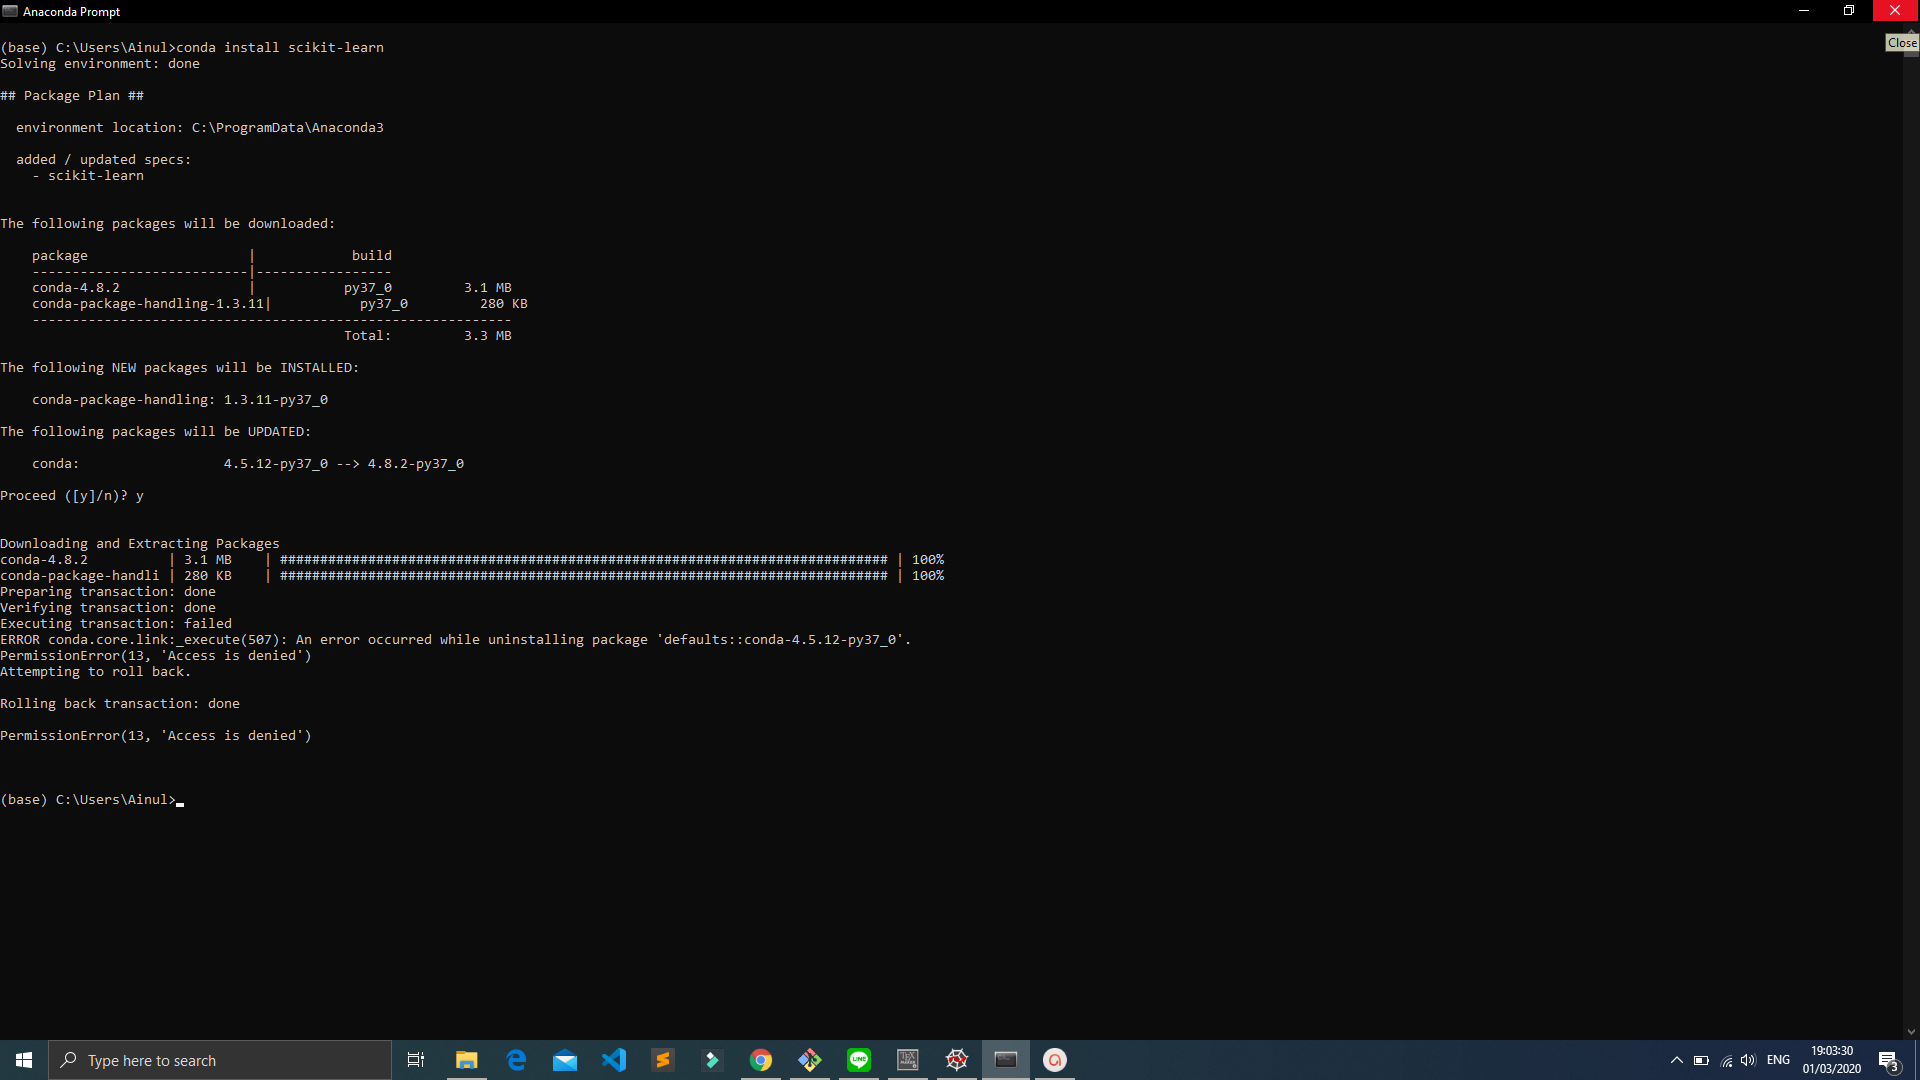
\includegraphics[width=4cm]{figures/1174073/1/1.PNG}
		\centering
		\caption{Instalasi Package Scikit Learn}
	\end{figure}
	\begin{figure}[H]
		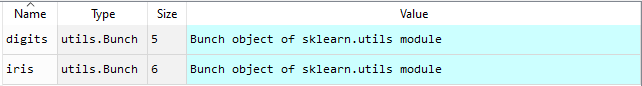
\includegraphics[width=4cm]{figures/1174073/1/2.png}
		\centering
		\caption{Isi Variabel Explorer}
	\end{figure}
	\item Mencoba Loading an example dataset, menjelaskan maksud dari tulisan tersebut dan mengartikan           		  per baris
	\hfill\break
	\lstinputlisting[firstline=7, lastline=11]{src/1174073/1/1174073.py}
	\item Mencoba Learning and predicting, menjelaskan maksud dari tulisan tersebut dan mengartikan per  			  baris
	\hfill\break
	\lstinputlisting[firstline=13, lastline=22]{src/1174073/1/1174073.py}
	\item  Mencoba Model persistence, menjelaskan maksud dari tulisan tersebut dan mengartikan per baris
	\hfill\break
	\lstinputlisting[firstline=25, lastline=34]{src/1174073/1/1174073.py}
	\item Mencoba Conventions, menjelaskan maksud dari tulisan tersebut dan mengartikan per baris
	\hfill\break
	\lstinputlisting[firstline=37, lastline=48]{src/1174073/1/1174073.py}
\end{enumerate}

\subsection{Penanganan Error}
\begin{enumerate}
	\item ScreenShoot Error
	\begin{figure}[H]
		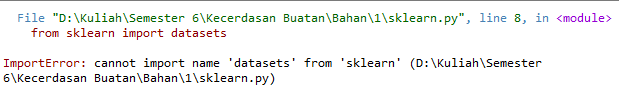
\includegraphics[width=4cm]{figures/1174073/1/error/1.png}
		\centering
		\caption{Import Error}
	\end{figure}

	\item Tuliskan Kode Error dan Jenis Error
	\begin{itemize}
		\item Import Error
	\end{itemize}
	\item Cara Penangan Error
	\begin{itemize}
		\item Import Error
		\hfill\break
		Dengan Menginstall Library Yang Tidak Ditemukan
	\end{itemize}
\end{enumerate}

\subsection{Bukti Tidak Plagiat}
\begin{figure}[H]
	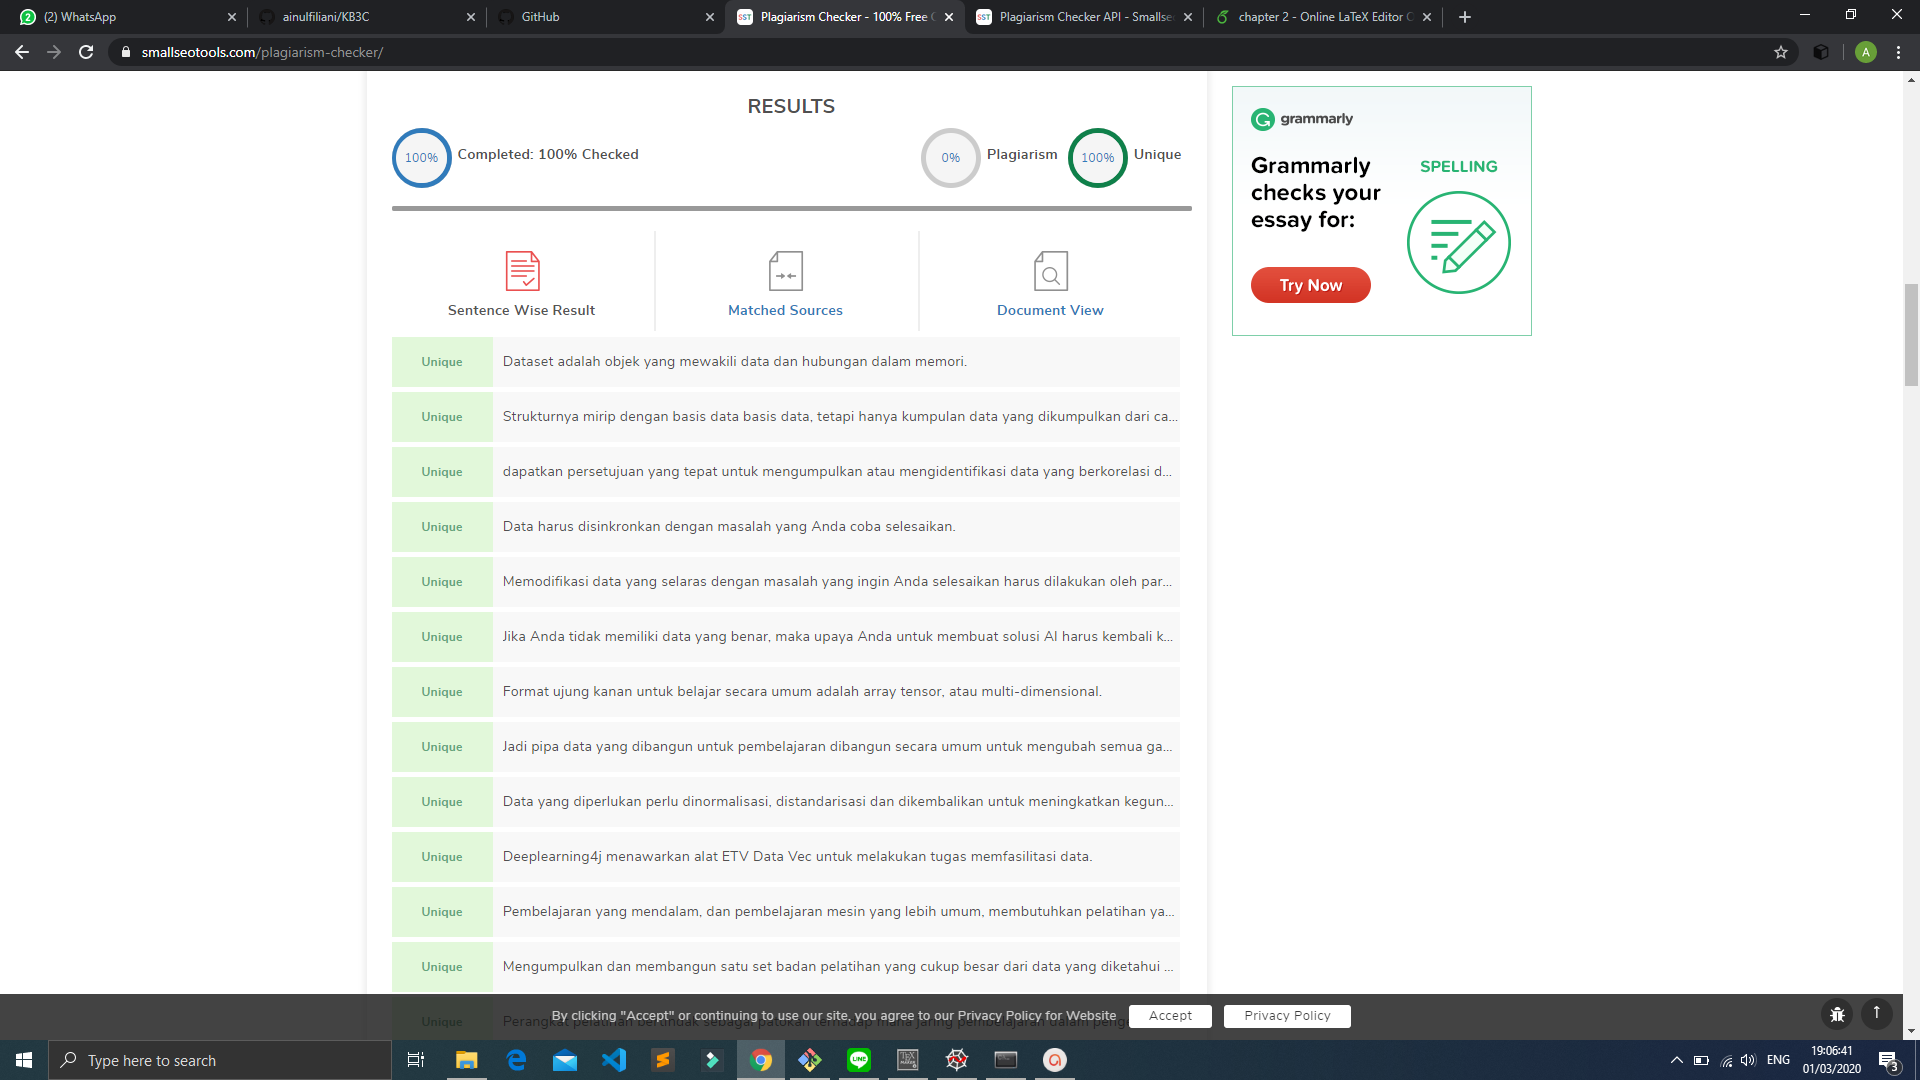
\includegraphics[width=4cm]{figures/1174073/1/plagiat/plagiat.PNG}
	\centering
	\caption{Bukti Tidak Melakukan Plagiat Chapter 1}
\end{figure}

\subsection{Link Youtube}
https://youtu.be/Ra4Lu-C8OQY


\section{Chandra Kirana Poetra (1174079)}
\subsection{Teori}
\begin{enumerate}
\item Definisi Kecerdasan buatan\\ 
Dalam bidang komputer, Aritificial Intelligence (AI), atau biasa disebut juga sebagai Machine Intelligence merupakan bentuk dari representasi kecerdasan yang dilakukan oleh mesin, hampir mirip seperti bagaimana manusia melakukan kecerdasan. Beberapa sumber mendefinisikan  bahwa bidang yang mempelajari suatu agen kecerdasan merupakan suatu alat yang mengenali lingkungan sekitarnya dan mencoba untuk membuat kesimpulan untuk memaksimalkan kemungkinan tingkat keberhasilan dari pencapaian yang ingin dituju.

\item Sejarah dan Perkembangan Kecerdasan Buatan
\begin{itemize}
\item Pada tahun 1943, pekerjaan pertama yang dikenal sebagai AI telah dilakukan oleh Warren McCulloch dan juga Walter Pits yang dinamakan sebagai artificial neurons
\item Pada tahun 1955, Allen Newell dan Herbert A. Simon membuat program kecerdasan buatan pertama yang dinamakan Logic Theorist
\item Pada tahun 1972, robot pertama dibuat di jepang dengan nama Wabot-1 dengan kecerdasan buatan
\item Pada tahun 1980, muncul bidang baru dari kecerdasan buatan yaitu Expert System yang membantu dalam pemberian keputusan
\item Tahun 1997, IBM deep blue mengalahkan juara catur dunia Gary Kasparov dan menjadi komputer pertama yang mengalahkannya
\item Tahub 2006, perusahaaan sudah mulai menerapkan kecerdasan buatan pada produknya seperti Netflix dan Twitter.
\item Tahun 2018,  	Project Debater dari IBM melakuakn debat tentang topik yang kompleks dan berakhir dengan hasil memuaskan
\end{itemize}

\item Definisi Supervised Learning\\
Supervised Learning adalah proses untuk melatih mesin secara input dan output melalui contoh nyata secara langsung

\item Klasifikasi Supervised Learning
\begin{itemize}
\item Support Vector Machines
\item linear regression
\item logistic regression
\item naive Bayes
\item linear discriminant analysis
\item decision trees
\item k-nearest neighbor algorithm
\item Neural Networks (Multilayer perceptron)
\item Similarity learning
\end{itemize}

\item Regresi dan Unsupervised Learning\\
Regresi adalah suatu proses statistikal yang mengestimasi hubungan antara variable satu dengan variable yang lainnya.

Unsupervised Learning adalah bentuk dari machine learning yang mencari bentuk atau hubungan dari data set yang tidak mempunyai label dengan bantuan yang minimal dari manusia.

\item Dataset\\
Dataset adalah koleksi suatu data

\item Training Set\\
Training Set merupakan data yang digunakan untuk keperluan pembelajaran yang biasanya digunakan oleh machine learning

\item Testing Set\\
Testing set adalah data yang real yang digunakan untuk melatih machine learning

\end{enumerate}

\subsection{Instalasi}
\begin{enumerate}
	\item Instalasi Library scikit dari a naconda, mencoba kompilasi dan uji coba ambil contoh kode dan lihat variabel explorer
	\hfill\break
	\begin{figure}[H]
		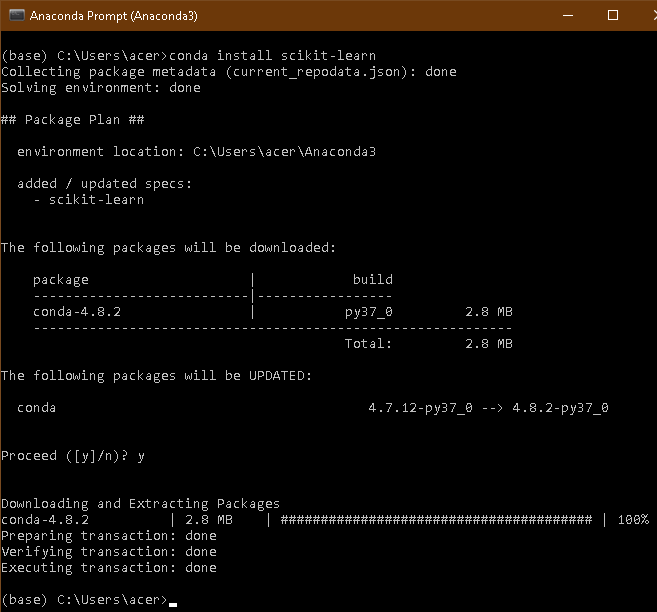
\includegraphics[width=4cm]{figures/1174079/1/1.PNG}
		\centering
		\caption{Instalasi Package Scikit Learn}
	\end{figure}
	\begin{figure}[H]
		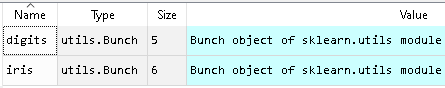
\includegraphics[width=4cm]{figures/1174079/1/2.png}
		\centering
		\caption{Isi Variabel Explorer}
	\end{figure}
	\item Mencoba Loading an example dataset, menjelaskan maksud dari tulisan tersebut dan mengartikan           		  per baris
	\hfill\break
	\lstinputlisting[firstline=2, lastline=7]{src/1174079/1/1174079.py}
	\item Mencoba Learning and predicting, menjelaskan maksud dari tulisan tersebut dan mengartikan per  			  baris
	\hfill\break
	\lstinputlisting[firstline=9, lastline=28]{src/1174079/1/1174079.py}
	\item  Mencoba Model persistence, menjelaskan maksud dari tulisan tersebut dan mengartikan per baris
	\hfill\break
	\lstinputlisting[firstline=30, lastline=48]{src/1174079/1/1174079.py}
	\item Mencoba Conventions, menjelaskan maksud dari tulisan tersebut dan mengartikan per baris
	\hfill\break
	\lstinputlisting[firstline=50, lastline=72]{src/1174079/1/1174079.py}
\end{enumerate}

\subsection{Penanganan Error}
\begin{enumerate}
	\item ScreenShoot Error
	\begin{figure}[H]
		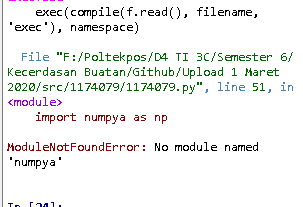
\includegraphics[width=4cm]{figures/1174079/1/error.png}
		\centering
		\caption{No Module Named Numpya}
	\end{figure}

	\item Tuliskan Kode Error dan Jenis Error
	\begin{itemize}
		\item ModuleNotFoundError
	\end{itemize}
	\item Cara Penangan Error
	\begin{itemize}
		\item ModuleNotFoundError
		\hfill\break
		Mengecek Typo dan menulis kembali library yang akan diimport
	\end{itemize}
\end{enumerate}

\subsection{Bukti Tidak Plagiat}
\begin{figure}[H]
	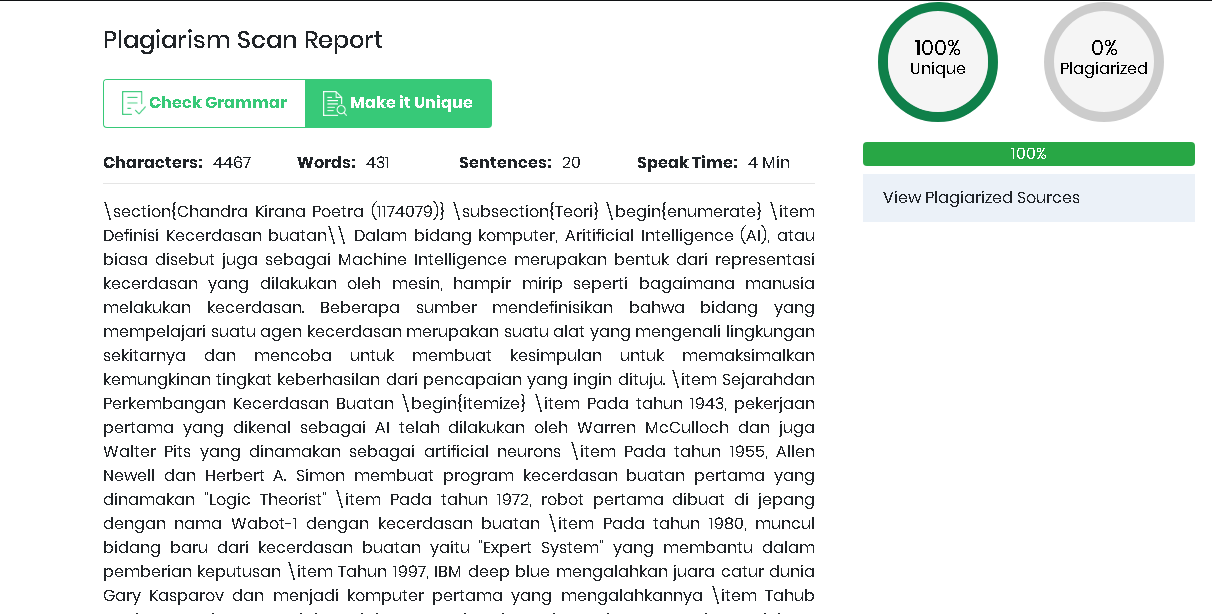
\includegraphics[width=4cm]{figures/1174079/1/plagiarism.PNG}
	\centering
	\caption{Bukti Tidak Melakukan Plagiat Chapter 1}
\end{figure}

\subsection{Link Youtube}
https://youtu.be/nPua0lRXjO8

\section{D. Irga B. Naufal Fakhri}
\subsection{Teori}
\subsubsection{Definisi Kecerdasan Buatan}

Kecerdasan Buatan atau yang sering disebut AI (Artificial Intelligence) merupakan suatu cabang didalam bisnis sains dan komputer sains yang didalamnya membahas tentang bagaimana caranya untuk membuat sebuah komputer dengan kemampuan atau kepintaran layaknya atau mirip dengan yang dimiliki manusia. 
Contohnya, bagaimana komputer bisa berkomunikasi dengan pengguna baik menggunakan kata, suara ataupun yang lainnya. 
Dengan kemampuan ini, diharapkan komputer dapat mengambil keputusan dengan sendirinya untuk memecahkan berbagai kasus yang ditemuinya kemudian itulah yang disebut dengan kecerdasan buatan. 
Kecerdasan buatan adalah kemampuan komputer digital atau robot yang dikendalikan konputer untuk melakukan tugas yang umumnya dikaitkan dengan sesuatu yang cerdas. Istilah ini sering diterapkan pada proyek pengembangan sistem yang diberkahi dengan karakteristik proses intelektual manusia, seperti kemampuan untuk berpikir, menemukan makna, menggeneralisasi, atau belajar dari pengalaman masa lalu.

Kecerdasan Buatan (AI) merupakan salah satu bidang yang sangat berhubungan dengan memanfaatkan mesin (komputer) untuk memecahkan suatu masalah atau persoalan yang rumit dengan cara yang lebih mudah dimengerti oleh manusia. Kecerdasan Buatan (AI) yang semakin canggih yang mampu menambahkan pengetahuannya dengan cara melakukan banyak testing dan perkembangan dari target yang di analisa. Contoh dari kecerdasan buatan yang paling terkenal saat ini adalah Google Assistant, Alexa dan Siri. Google Assisntant, Alexa dan Siri sangat dikenal karena penggunaannya yang mudah oleh user untuk menemukan berbagai hal atau membuatnya untuk melakukan sesuatu terhadap smartphone atau smarthome anda dan contohnya masih banyak lagi.

\subsubsection{Sejarah Kecerdasan Buatan}

Kecerdasan Buatan (Artificial intelligence) mulai dibentuk sejak adanya komputer modern yang diperkirakan terjadi pada tahun 1940 dan 1950. Ilmu pengetahuan kecerdasan buatan ini dikhususkan dalam perancangan otomatisasi tingkah laku cerdas dalam sistem kecerdasan komputer. 

Pada awal 50-an, studi tentang “mesin berpikir” memiliki berbagai nama seperti cybernetics, teori automata, dan pemrosesan innformasi. 
Pada tahun 1956, para ilmuan jenius seperti Alan Turing, Norbert, Wiener, Claude Shannon dan Warren McCullough telah bekerja secara independen dibidang cybernetics, matematika, algoritma dan teori jaringan. Namun, seprang ilmuan komputer dan kognitif John McCarthy adalah orang yang dating dengan ide untuk bergabung dengan upaya penelitian terpisah ini kedalam satu bidang yang akan mempelajari topic baru untuk imajinasi manusia yaitu kecerdasan buatan. Dia adalah orang yang menciptakan istilah tersebut dan kemudian mendirikan laboratorium Kecerdasan Buatan di MIT dan Stan ford.
Pada tahun 1956, McCarthy yang sama mendirikan Konferensi Dartmouth di Hanover, New Hampshire. Peneliti terkemuka dalam teori kompleksitas, simulasi bahasa, hubungan antara keacakan dan pemikiran kreatif, jaringan saraf diundang. Tujuan dari bidang penelitian yang baru dibuat adalah untuk mengembangkan mesin yang dapat mensimulasikan setiap aspek kecerdasab. Itulah sebabnya Konferensi Dartmouth 1956 dianggap sebagai kelahiran Kecerdasan Buatan. Sejak saat itu, Kecerdasa Buatan telah hidup melalui decade kemuliaan dan cemoohan, yang dikenal luas sebagai musim panas dan musim dingin AI. Musim panasnya ditandai dengan optimism dan dana besar, sedangkan musim dinginnya dihadapkan dengan pemotongan dana, ketidakkpercayaan dan pesimisme.

\subsubsection{Perkembangan Kecerdasan Buatan}

Teknologi Artificial Intelligence semakin ramai dibahas dalam berbagai diskusi teknologi di seluruh dunia.Menurut kebanyakan orang, pekerjaan seperti kasir, operator telepon, pengendara truk, dan lainnya sangat berpeluang besar untuk tergantikan oleh Artificial Intelligence. Mengapa terjadi hal demikian? dikarenakan memang bahwa AI lebih ungul dalam hal kinerja, fitur dan lain sebagainya. Namun, dalam beberapa aspek memang pekerja manusia masih unggul dibandingkan AI itu sendiri. Para generasi muda yang ada di dunia terutama di daerah Asia terlihat sudah memahami fungsi dan efek dari AI dalam kehidupan kita sehari-hari. Berdasarkan survei yang dilakukan oleh Microsoft, terdapat 39 persen responden yang mempertimbangkan untuk menggunakan mobil tanpa pengemudi dan 36 persen lainnya setuju bahwa robot masa depan dengan software untuk beroperasi mampu meningkatkan produktivitas. Dari survey tersebut kita sebagai pengguna AI harus lebih bijaksana dalam pengembangan dan penggunaan dari AI sehingga tanpa memberikan efek samping terhadap etos kerja dan keseharian kita sebagai pengguna dalam kehidupan sehari-hari.

AI Summer 1 (1956-1973) KOnferensi Dartmounth diikuti oleh 17 tahun kemajuan luar biasa. Proyek penelitian yang dilakukan di MIT, universitas di Edinburgh, Stanford dan Carnegie Mellon menerima dana besar-besaran, yang akhirnya membuahkan hasil. Selama tahun-tahun itulah komputer pemrograman mulai melakukan masalah aljabar, membuktikan teorema geometris, memahami dan menggunakan sintaks dan tata bahasa Inggris. Terlepas dari ditinggalkannya koneksionisme dan terjemahan mesin yang gagal, yang menunda penelitian Natural Language Processing (NLP) selama bertahun-tahun, banyak prestasi dari masa lalu yang membuat sejarah. Berikut ini beberapa diantaranya : Pelopor pembelajaran mesin, Ray Solomonoff meletakkan dasar-dasar teori metematika AI, memperkenalkan metode Bayesian universal untuk inferensi dan preddiksi induktif Thomas Evans menciptakan program ANALOGI heuristik, yang memungkinkan komputer memecahkan masalah geometri-analogi Unimation, perusahaan robotika pertma didunia, menciptakan robot industri Unimate, yang bekerja pada jalur perakitan modil Genenral Motors. Joseph Weizenbaum membangun ELIZA-program interaktif yang dapat membawa percakapan dalam bahasan Inggris tentang topik apapun. Ross Quillian menunjukkan jaring semanik, sedangkan Jaime Carbonell (Sr.) mengembangkan Cendikia-program interaktif untuk instruksi yang dibantu komputer berdasarkan jaring semantik. Edward Feigenbaum dan Julian Feldman menerbitkan Computeks and Thought, kumpulan artikel pertama tentang AI.

\subsubsection{Supervised Learning}
Supervised Learning adalah tugas pengumpulan data untuk menyimpulkan fungsi dari data pelatihan berlabel. Data pelatihan terdiri dari serangkaian contoh pelatihan. Dalam supervised learning, setiap contoh adalah pasangan yang terdiri dari objek input (biasanya vektor) dan nilai output yang diinginkan(juga disebut sinyal pengawasan super). Algoritma pembelajaran yang diawasi menganalisis data pelatihan dan menghasilkan fungsi yang disimpulkan, yang dapat digunakan untuk memetakan contoh-contoh baru. Skenario optimal akan memungkinkan algoritma menentukan label kelas dengan benar untuk instance yang tidak terlihat. Ini membutuhkan algoritma pembelajaran untuk menggeneralisasi dari data pelatihan untuk situasi yang tidak terlihat dengan cara yang "masuk akal". Supervised Learning adalah pendekatan dimana sudah terdapat data yang dilatih selain itu juga terdapat variable yang ditargetkan sehingga tujuan dari pendekatan ini yaitu mengelompokkan suatu data ke dta yang sudah ada. Supervised Learning menyediakan algoritma pembelajaran dengan jumlah yang diketahui untuk mendukung penilaian dimasa depan. Chatbots, mobil self-driving, program pengenalan wajah, sistem pakar dan robot adalah beberapa sistem yang dapat menggunakan pembelajaran yang diawasi atau tidak diawasi. Supervised Learning sebagian besar terkait dengan AI berbasis pengambilan tetapi mereka juga mungkin mampu menggunakan model pembelajaran generatif. Data pelatihan untuk pembelajaran yang diawasi mencakup serangkaian contoh dengan subjek input berpasangan dan output yang diinginkan (yang juga disebut sebagai sinyal pengawasan).

Dalam pembelajaran yang diawasi untuk pemrosesan gambar, misalnya sistem AI mungkin dilengkapi dengan gambar berlabel kendaraan dalam ketegori seperti mobil dan truk. Setelah jumlah pengamatan yang cukup, sistem harus dapat membedakan antara dan mengkategorikan gambar yang tidak berlabel, dimana waktu pelatihan dapat dikatakan lengkap. Model Supervised Learning memiliki beberapa keunggulan dibandingkan pendekatan tanpa pengawasan, tetapi mereka juga memiliki keterbatasan. Sistem lebih cenderung membuat penilaian bahwa manusia dapat berhubungan, misalnya karena manusia telah memberikan dasar untuk keputusan. Namun, dalam kasus metode berbasis pengambilan, Supervised Learning mengalami kesulitan dalam menangani informaasi baru. Jika suatu sistem dengan kategori untuk mobil dan truk disajikan dengan sepeda, misalnya ia harus salah dikelompokkan dalam satu kategori ata yang lain. Namun. jika sistem AI bersifat generatif, ia mungkin tidak tahu apa sepeda itu tetapi akan dapat mengenalinya sebagai milik kategori yang terpisah.

\subsubsection{Klasifikasi}
Klasifikasi adalah pembagian sesuatu menurut kelas-kelas ( class ). Menurut Ilmu Pengetahuan, Klasifikasi merupakan proses pengelompokkan benda berdasarkan ciri-ciri persamaan dan juga perbedaan. Dalam masalah klasifikasi, kami mencoba memprediksi sejumlah nilai terpisah. Label (y) umumnya datang dalam bentuk kategorikal dan mewakili sejumlah kelas. Dalam pembelajaran mesin dan statistik, klasifikasi adalah pendekatan pembelajaran yang diawasi di mana program komputer belajar dari input data yang diberikan kepadanya dan kemudian menggunakan pembelajaran ini untuk mengklasifikasikan pengamatan baru. Kumpulan data ini mungkin hanya bersifat dua kelas (seperti mengidentifikasi apakah orang tersebut berjenis kelamin laki-laki atau perempuan atau bahwa surat itu spam atau bukan-spam) atau mungkin juga multi-kelas. Beberapa contoh masalah klasifikasi adalah: pengenalan ucapan, pengenalan tulisan tangan, identifikasi metrik, klasifikasi dokumen dll.

\subsubsection{Regresi}
Regresi adalah metode analisis statistik yang digunakan untuk melihat pengaruh antara dua ataupun lebih variabel. Regresi adalah membahas masalah ketika variabel output adalah nilai riil atau berkelanjutan, seperti "gaji" atau "berat". Banyak model yang berbeda dapat digunakan makan, yang paling sederhana adalah regresi linier. Ia mencoba untuk menyesuaikan data dengan hyper-plane terbaik yang melewati poin.

\subsubsection{Unsupervised Learning}
Unsupervised Learning berbeda dengan Supervised Leraning. Perbedaannya ialah unsupervised learning tidak memiliki data latih, sehingga dari data yang ada kita mengelompokan data tersebut menjadi 2 ataupun 3 bagian dan seterusnya. Unsupervised Learning adalah pelatihan algoritma kecerdasan buatan (AI) menggunakan informasi yang tidak diklasifikasikan atau diberi label dan memungkinkan algoritma untuk bertindak atas informasi tersebut tanpa bimbingan. Dalam Unsupervised Learning, sistem AI dapat mengelompokkan informasi yang tidak disortir berdasarkan persamaan dan perbedaan meskipun tidak ada kategori yang disediakan.

Dalam Unsupervised Learning, sistem AI disajikan dengan data yang tidak berlabel, tidak terkategorisasi dan algoritma sistem bekerja pada data tanpa pelatihan sebelumnya. Outputnya tergantung pada algoritma kode. Menundukkan suatu sistem pada Unsupervised Learning adalah salah satu cara untuk menguji AI. Algoritma Unsupervised Learning dapat melakukan tugas pemrosesan yang lebih kompleks daripada sistem pembelajaran yang
diawasi. Namun, pembelajaran tanpa pengawasan bisa lebih tidak terduga daripada model alternatif. Sementara Unsupervised Learningi mungkin, misalnya, mencari tahu sendiri cara memilah kucing dari anjing, mungkin juga menambahkan kategori yang tidak terduga dan tidak diinginkan untuk menangani breed yang tidak biasa, membuat kekacauan bukannya keteraturan


\subsubsection{Data Set}
Dataset adalah objek yang merepresentasikan data dan juga relasi yang ada di memory. Strukturnya mirip dengan data di database, namun bedanya
dataset berisi koleksi dari data table dan data relation. mendapatkan data yang tepat berarti mengumpulkan atau mengidentifikasi data yang berkorelasi dengan hasil yang ingin Anda prediksi; yaitu data yang berisi sinyal tentang peristiwa yang Anda pedulikan. Data harus diselaraskan dengan masalah yang Anda coba selesaikan. Gambar kucing tidak terlalu berguna ketika Anda sedang membangun sistem identifikasi wajah. Memverifikasi bahwa data selaras dengan masalah yang ingin Anda selesaikan harus dilakukan oleh ilmuwan data. Jika Anda tidak memiliki data yang tepat, maka upaya Anda untuk membangun solusi AI harus kembali ke tahap pengumpulan data. Format ujung kanan untuk pembelajaran dalam umumnya adalah tensor, atau array multi-dimensi. Jadi jalur pipa data yang dibangun untuk pembelajaran mendalam umumnya akan mengkonversi semua data - baik itu gambar, video, suara, suara, teks atau deret waktu  menjadi vektor dan tensor yang dapat diterapkan operasi aljabar linier. Data itu seringkali perlu dinormalisasi, distandarisasi dan dibersihkan untuk meningkatkan kegunaannya, dan itu semua adalah langkah dalam ETL pembelajaran mesin. Deeplearning4j menawarkan alat ETV DataVec untuk melakukan tugas-tugas pemrosesan data tersebut.

Pembelajaran yang dalam, dan pembelajaran mesin yang lebih umum, membutuhkan pelatihan yang baik agar bekerja dengan baik. Mengumpulkan dan membangun set pelatihan  badan yang cukup besar dari data yang diketahui  membutuhkan waktu dan pengetahuan khusus domain tentang di mana dan bagaimana mengumpulkan informasi yang relevan. Perangkat pelatihan bertindak sebagai tolok ukur terhadap mana jaring pembelajaran dalam dilatih. Itulah yang mereka pelajari untuk direkonstruksi sebelum mereka melepaskan data yang belum pernah mereka lihat sebelumnya. Pada tahap ini, manusia yang berpengetahuan luas perlu menemukan data mentah yang tepat dan mengubahnya menjadi representasi numerik yang dapat dipahami oleh algoritma pembelajaran mendalam, tensor. Membangun set pelatihan, dalam arti tertentu, pra-pra pelatihan. Set pelatihan yang membutuhkan banyak waktu atau keahlian dapat berfungsi sebagai keunggulan dalam dunia ilmu data dan pemecahan masalah. Sifat keahlian sebagian besar dalam memberi tahu algoritma Anda apa yang penting bagi Anda dengan memilih apa yang masuk ke dalam set pelatihan. Ini melibatkan menceritakan sebuah kisah  melalui data awal yang Anda pilih yang akan memandu jaring pembelajaran mendalam Anda saat mereka mengekstraksi fitur-fitur penting, baik di set pelatihan maupun dalam data mentah yang telah mereka ciptakan untuk dipelajari. Untuk membuat set pelatihan yang bermanfaat, Anda harus memahami masalah yang Anda selesaikan; yaitu apa yang Anda inginkan agar jaring pembelajaran mendalam Anda memperhatikan, di mana hasil yang ingin Anda prediksi.


\subsubsection{Training Set}
Training Set adalah set digunakan oleh algoritma klassifikasi . Dapat dicontohkan dengan : decision tree, bayesian, neural network dll. Semuanya dapat digunakan untuk membentuk sebuah model classifier. Menjalankan pelatihan yang diatur melalui jaringan saraf mengajarkan pada net
cara menimbang berbagai fitur, menyesuaikan koefisien berdasarkan kemungkinan mereka meminimalkan kesalahan dalam hasil Anda. Koefisien-koefisien tersebut, juga dikenal sebagai parameter, akan terkandung dalam tensor dan bersama-sama mereka disebut model, karena mereka mengkodekan model data yang mereka latih. Mereka adalah takeaways paling penting yang akan Anda dapatkan dari pelatihan jaringan saraf.


\subsubsection{Testing Set}
Testing Set adalah set yang digunakan untuk mengukur sejauh mana classifier berhasil melakukan klasifikasi dengan benar. Ini berfungsi sebagai meterai persetujuan, dan Anda tidak menggunakannya sampai akhir. Setelah Anda melatih dan mengoptimalkan data Anda, Anda menguji jaringan saraf Anda terhadap pengambilan sampel acak akhir ini. Hasil yang dihasilkannya harus memvalidasi bahwa jaring Anda secara akurat mengenali gambar, atau mengenalinya setidaknya [x] dari jumlah tersebut. Jika Anda tidak mendapatkan prediksi yang akurat, kembalilah ke set pelatihan, lihat hyperparameter yang Anda gunakan untuk menyetel jaringan, serta kualitas data Anda dan lihat teknik pra-pemrosesan Anda.

\subsection{Praktek}
\subsubsection{Instalasi library scikit dari anaconda, mencoba kompilasi dan uji coba ambil contoh kode dan lihat variabel explorer}
\begin{enumerate}

\item Pastikan anda telah menginstall anaconda lalu buka aplikasi Anaconda Prompt

\item Lalu pastikan anda telah menginstall python

\item Pada Anaconda Prompt install scikit dengan cara conda install scikit-learn
\begin{figure}[H]
	\begin{center}
   	 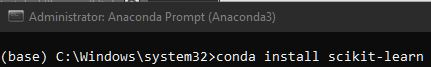
\includegraphics[width=10cm]{figures/1174066/1/1.png}
   	 \caption{Instalasi Scikit Dari Anaconda Prompt}	
	\end{center}
\end{figure}

\item Lalu tulis kode yang ada dibawah ini dan run menggunakan spyder
\lstinputlisting[firstline=1, lastline=4]{src/1174066/1/contoh.py}
\begin{figure}[H]
	\begin{center}
   	 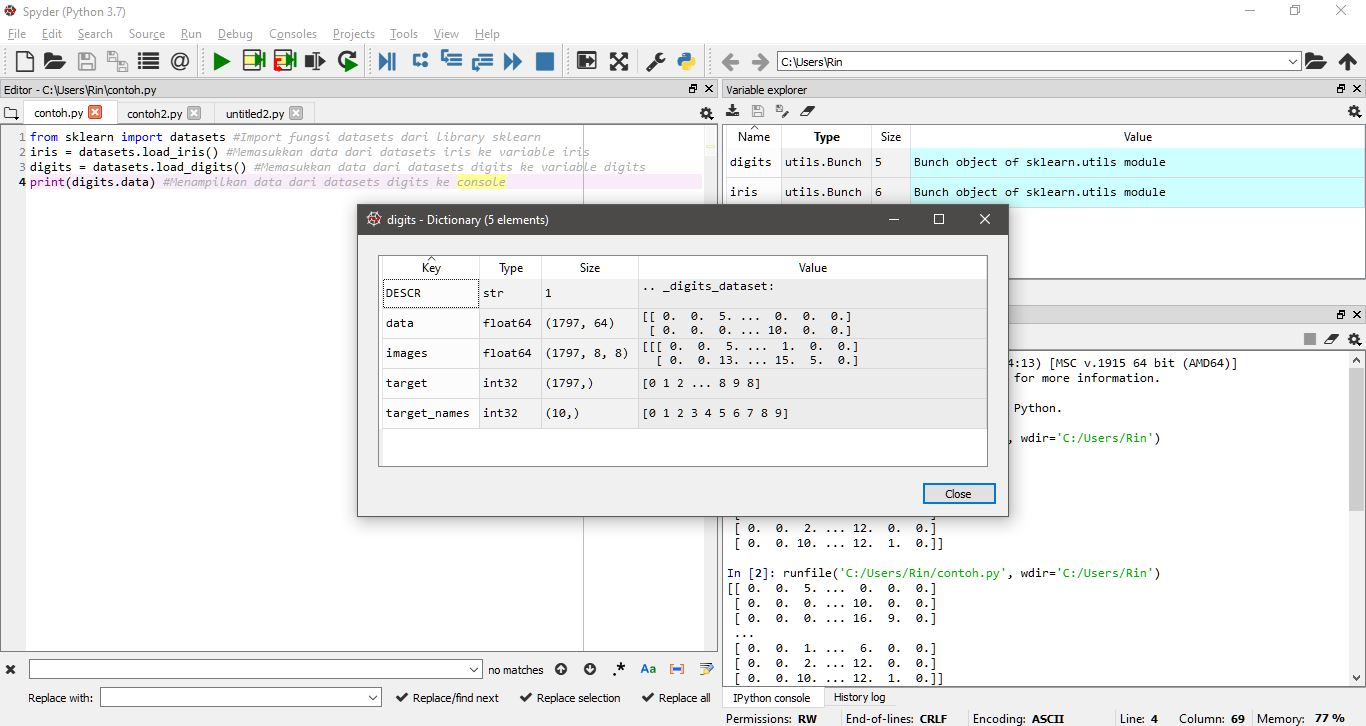
\includegraphics[width=10cm]{figures/1174066/1/2.png}
   	 \caption{Running Kode dari Spyder dan Hasil Variable Explorer}	
	\end{center}
\end{figure}
\end{enumerate}

\subsubsection{Loading an example dataset}
\begin{figure}[H]
	\begin{center}
   	 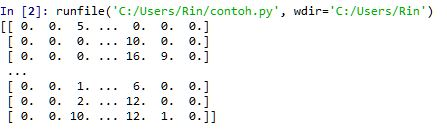
\includegraphics[width=10cm]{figures/1174066/1/3.png}
   	 \caption{Running Loading an example dataset dari Spyder}	
	\end{center}
\end{figure}

\begin{itemize}
\item Import fungsi datasets dari library sklearn
\lstinputlisting[firstline=1, lastline=1]{src/1174066/1/contoh.py}

\item Memasukkan data dari datasets iris ke variable iris
\lstinputlisting[firstline=2, lastline=2]{src/1174066/1/contoh.py}

\item Memasukkan data dari datasets digits ke variable digits
\lstinputlisting[firstline=3, lastline=3]{src/1174066/1/contoh.py}

\item Menampilkan data dari datasets digits ke console
\lstinputlisting[firstline=4, lastline=4]{src/1174066/1/contoh.py}
\begin{figure}[H]
	\begin{center}
   	 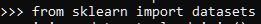
\includegraphics[width=10cm]{figures/1174066/1/5.png}
   	 \caption{Hasil Running kode loading an example dataset}	
	\end{center}
\end{figure}
\end{itemize}

\subsubsection{Learning and predicting}
\begin{itemize}
\item Buka Anaconda Prompt
\begin{figure}[H]
	\begin{center}
   	 
\includegraphics[width=10cm]{figures/1174066/1/anaconda.png}
   	 \caption{Anaconda Prompt}	
	\end{center}
\end{figure}

\item Lalu kita import datasets dari sklearn seperti dibawah ini
\begin{figure}[H]
	\begin{center}
   	 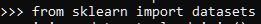
\includegraphics[width=10cm]{figures/1174066/1/5.png}
   	 \caption{Menggunakan datasets}	
	\end{center}
\end{figure}

\item lalu kita mendefisisikan iris dan digits menjadi variable
\begin{figure}[H]
	\begin{center}
   	 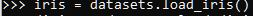
\includegraphics[width=10cm]{figures/1174066/1/6.png}
   	 \caption{mendefinisikan iris}	
	\end{center}
\end{figure}
\begin{figure}[H]
	\begin{center}
   	 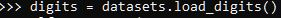
\includegraphics[width=10cm]{figures/1174066/1/7.png}
   	 \caption{mendefinisikan digits}	
	\end{center}
\end{figure}

\item Lalu kita import svm dari sklearn yang nantinya digunakan untuk menjadi estimanasi angka kita
\begin{figure}[H]
	\begin{center}
   	 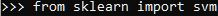
\includegraphics[width=10cm]{figures/1174066/1/4.png}
   	 \caption{Menggunakan svm}	
	\end{center}
\end{figure}

\item Lalu, kita definisikan clf sebagai classfier, disini gamma didefinisikan secara manual
\begin{figure}[H]
	\begin{center}
   	 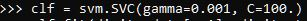
\includegraphics[width=10cm]{figures/1174066/1/8.png}
   	 \caption{Mendefinisikan Classifier}	
	\end{center}
\end{figure}

\item Estimator clf (for classifier) pertama kali dipasang pada model. Ini dilakukan dengan melewati training set ke metode fit. Untuk training set, akan menggunakan semua gambar dari set data yang ada, kecuali untuk gambar terakhir, yang dicadangan untuk prediksi. Pada skrip dibawah memilih training set dengan sintaks Python [: -1], yang menghasilkan array baru yang berisi semua kecuali item terakhir dari digits.
\begin{figure}[H]
	\begin{center}
   	 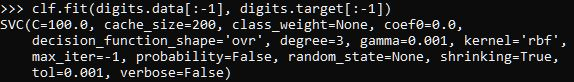
\includegraphics[width=10cm]{figures/1174066/1/9.png}
   	 \caption{Memanggil Classifier}	
	\end{center}
\end{figure}

\item Menunnjukkan prediksi angka baru
\begin{figure}[H]
	\begin{center}
   	 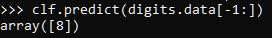
\includegraphics[width=10cm]{figures/1174066/1/10.png}
   	 \caption{Prediksi nilai baru}	
	\end{center}
\end{figure}
\end{itemize}
\lstinputlisting[firstline=8 lastline=15]{src/1174066/1/contoh2.py}

\subsubsection{Model Persistance}
Model Persistance
\lstinputlisting[firstline=8 lastline=32]{src/1174066/1/contoh3.py}

\subsubsection{Conversion}
Conversion
\lstinputlisting[firstline=8 lastline=19]{src/1174066/1/contoh4.py}

\subsection{Penanganan Error}

Dari percobaan yang dilakukan di atas, apabila mendapatkan error maka:
\begin{enumerate}

\item Screenshoot Error
\begin{figure}[H]
	\begin{center}
   	 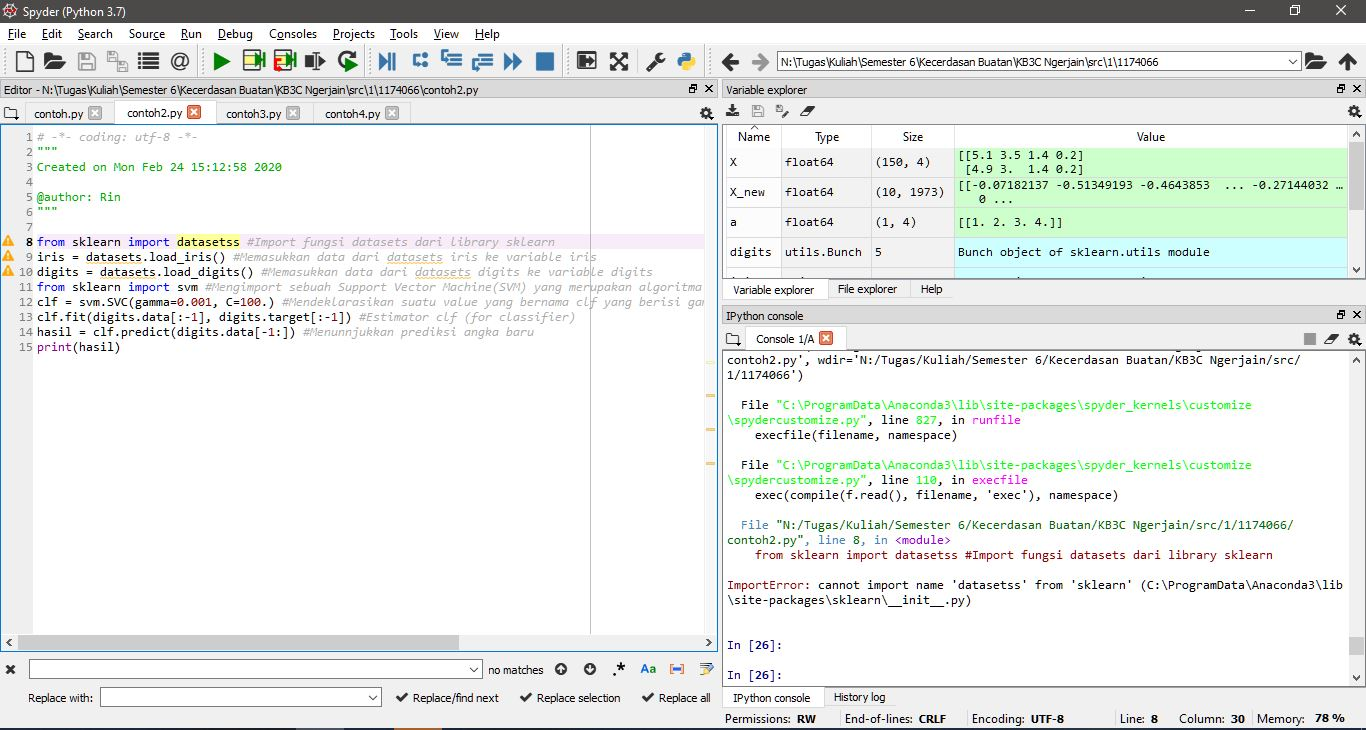
\includegraphics[width=10cm]{figures/1174066/1/error1.png}
   	 \caption{ImportError: cannot import name 'datasetss' from 'sklearn'}	
	\end{center}
\end{figure}
	
\item Tuliskan kode eror dan jenis errornya [hari ke 2](10)
\begin{itemize}
\item ImportError
\end{itemize}

\item Solusi pemecahan masalah error tersebut[hari ke 2](10)
\begin{itemize}
\item ImportError

Cek kembali jika ada yang typo
\end{itemize}

\end{enumerate}

\subsection{Bukti Tidak Plagiat}
\begin{figure}[H]
	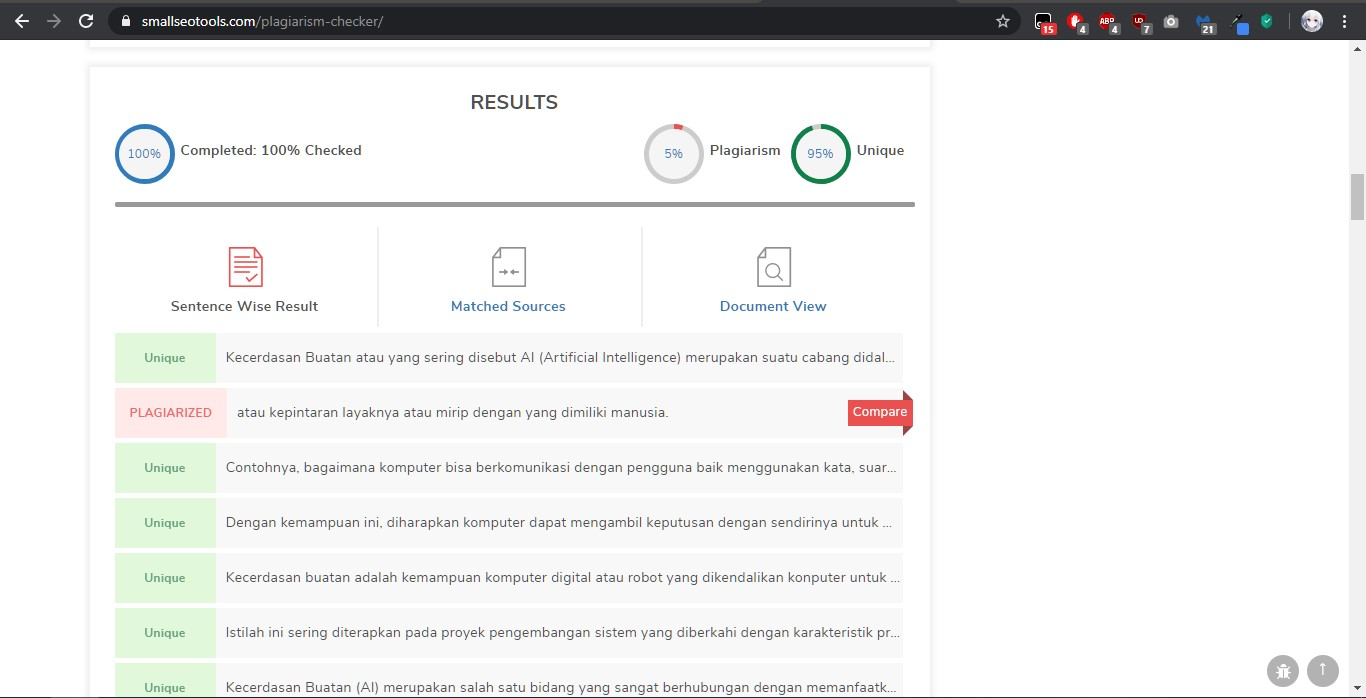
\includegraphics[width=4cm]{figures/1174066/1/plagiat.png}
	\centering
	\caption{Bukti Tidak Melakukan Plagiat Chapter 1}
\end{figure}

\subsection{Link Youtube}
https://youtu.be/S8Sj\_vZluUs
\section{1174087 - Ilham Muhammad Ariq}
\subsection{Teori}
\begin{enumerate}
	\item Definisi Kecerdasan Buatan
		\par Kecerdasan Buatan adalah suatu ilmu yang mempelajari bagaimana cara komputer melakukan sesuatu seperti yang dilakukan oleh manusia. Secara sederhana AI adalah teknik dan ilmu untuk membangun atau membuat suatu mesin menjadi cerdas, terutama pada program komputer. Kecerdasan yang dimaksud yaitu seperti yang dimiliki oleh manusia namun pada mesin akan dibuat cepat dan tepat atau akurat.

	\item {Sejarah Kecerdasan Buatan}
    \par Artificial intelligence merupakan inovasi baru di bidang ilmu pengetahuan. Mulai terbentuk sejak adanya komputer modern dan kira-kira terjadi sekitaran tahun 1940 dan 1950. Ilmu pengetahuan komputer ini khusus ditujukan dalam perancangan otomatisasi tingkah laku cerdas dalam sistem kecerdasan komputer. Pada awal 50-an, studi tentang “mesin berpikir” memiliki berbagai nama seperti cybernetics, teori automata, dan pemrosesan innformasi. Pada tahun 1956, para ilmuan jenius seperti Alan Turing, Norbert, Wiener, Claude Shannon dan Warren McCullough telah bekerja secara independen dibidang cybernetics, matematika, algoritma dan teori jaringan. Namun, seprang ilmuan komputer dan kognitif John McCarthy adalah orang yang dating dengan ide untuk bergabung dengan upaya penelitian terpisah ini kedalam satu bidang yang akan mempelajari topic baru untuk imajinasi manusia yaitu kecerdasan buatan. Dia adalah orang yang menciptakan istilah tersebut dan kemudian mendirikan laboratorium Kecerdasan Buatan di MIT dan Stan ford.

    Pada tahun 1956, McCarthy yang sama mendirikan Konferensi Dartmouth di Hanover, New Hampshire. Peneliti terkemuka dalam teori kompleksitas, simulasi bahasa, hubungan antara keacakan dan pemikiran kreatif, jaringan saraf diundang. Tujuan dari bidang penelitian yang baru dibuat adalah untuk mengembangkan mesin yang dapat mensimulasikan setiap aspek kecerdasab. Itulah sebabnya Konferensi Dartmouth 1956 dianggap sebagai kelahiran Kecerdasan Buatan. Sejak saat itu, Kecerdasa Buatan telah hidup melalui decade kemuliaan dan cemoohan, yang dikenal luas sebagai musim panas dan musim dingin AI. Musim panasnya ditandai dengan optimism dan dana besar, sedangkan musim dinginnya dihadapkan dengan pemotongan dana, ketidakkpercayaan dan pesimisme.

    \item{Perkembangan Kecerdasan Buatan}
    \par Teknologi Artificial Intelligence semakin ramai dibahas dalam berbagai diskusi teknologi di seluruh dunia.Menurut kebanyakan orang, pekerjaan seperti kasir, operator telepon, pengendara truk, dan lainnya sangat berpeluang besar untuk tergantikan oleh Artificial Intelligence. Mengapa terjadi hal demikian? dikarenakan memang bahwa AI lebih ungul dalam hal kinerja, fitur dan lain sebagainya. Namun, dalam beberapa aspek memang pekerja manusia masih unggul dibandingkan AI itu sendiri. Para generasi muda yang ada di dunia terutama di daerah Asia terlihat sudah memahami fungsi dan efek dari AI dalam kehidupan kita sehari-hari. Berdasarkan survei yang dilakukan oleh Microsoft, terdapat 39 persen responden yang mempertimbangkan untuk menggunakan mobil tanpa pengemudi dan 36 persen lainnya setuju bahwa robot masa depan dengan software untuk beroperasi mampu meningkatkan produktivitas. Dari survey tersebut kita sebagai pengguna AI harus lebih bijaksana dalam pengembangan dan penggunaan dari AI sehingga tanpa memberikan efek samping terhadap etos kerja dan keseharian kita sebagai pengguna dalam kehidupan sehari-hari.

    AI Summer 1 (1956-1973) KOnferensi Dartmounth diikuti oleh 17 tahun kemajuan luar biasa. Proyek penelitian yang dilakukan di MIT, universitas di Edinburgh, Stanford dan Carnegie Mellon menerima dana besar-besaran, yang akhirnya membuahkan hasil. Selama tahun-tahun itulah komputer pemrograman mulai melakukan masalah aljabar, membuktikan teorema geometris, memahami dan menggunakan sintaks dan tata bahasa Inggris. Terlepas dari ditinggalkannya koneksionisme dan terjemahan mesin yang gagal, yang menunda penelitian Natural Language Processing (NLP) selama bertahun-tahun, banyak prestasi dari masa lalu yang membuat sejarah. Berikut ini beberapa diantaranya : Pelopor pembelajaran mesin, Ray Solomonoff meletakkan dasar-dasar teori metematika AI, memperkenalkan metode Bayesian universal untuk inferensi dan preddiksi induktif Thomas Evans menciptakan program ANALOGI heuristik, yang memungkinkan komputer memecahkan masalah geometri-analogi Unimation, perusahaan robotika pertma didunia, menciptakan robot industri Unimate, yang bekerja pada jalur perakitan modil Genenral Motors. Joseph Weizenbaum membangun ELIZA-program interaktif yang dapat membawa percakapan dalam bahasan Inggris tentang topik apapun. Ross Quillian menunjukkan jaring semanik, sedangkan Jaime Carbonell (Sr.) mengembangkan Cendikia-program interaktif untuk instruksi yang dibantu komputer berdasarkan jaring semantik. Edward Feigenbaum dan Julian Feldman menerbitkan Computeks and Thought, kumpulan artikel pertama tentang AI.

	\item Definisi supervised learning, klasifikasi, regresi, unsupervised learning, dataset, training set dan testing set.
	\begin{itemize}
	\item Supervised Learning
		\par Supervised Learning merupakan sebuah tipe learning yang mempunyai variable input dan variable output, tipe ini juga menggunakan satu algoritma atau lebih dari satu algoritma yang digunakan untuk mempelajari fungsi  pemetaan dari input ke output.
		
	\item Klasifikasi
		\par Klasifikasi adalah pengelompokan data di mana data yang digunakan memiliki label atau kelas target. Sehingga algoritma untuk menyelesaikan masalah klasifikasi dikategorikan ke dalam pembelajaran terbimbing.
		
	\item Regresi
		\par Regresi metode analisis statistik yang digunakan untuk dapat melihat efek antara dua atau lebih variabel. Hubungan variabel dalam pertanyaan adalah fungsional yang diwujudkan dalam bentuk model matematika. Dalam analisis regresi, variabel dibagi menjadi dua jenis, yaitu variabel respons atau yang biasa disebut variabel dependen dan variabel independen atau dikenal sebagai variabel independen. Ada beberapa jenis analisis regresi, yaitu regresi sederhana yang mencakup linear sederhana dan regresi non-linear sederhana dan regresi berganda yang mencakup banyak linier atau non-linear berganda. Analisis regresi digunakan dalam pembelajaran mesin pembelajaran dengan metode pembelajaran terawasi.
		
	\item Unsupervised learning 
		\par Unsupervised learning jenis pembelajaran di mana kita hanya memiliki data input (input data) tetapi tidak ada variabel output yang terkait. Tujuan dari pembelajaran tanpa pengawasan adalah untuk memodelkan struktur dasar atau distribusi data dengan tujuan mempelajari data lebih lanjut, dengan kata lain, itu adalah fungsi simpulan yang menggambarkan atau menjelaskan data.
		
	\item Data set
		\par Data set objek yang merepresentasikan data dan relasinya di memory. Strukturnya mirip dengan data di database. Dataset berisi koleksi dari datatable dan datarelation.
		
	\item Training Set
		\par Training set adalah bagian dari dataset yang di latih untuk membuat prediksi atau menjalankan fungsi dari algoritma ML lain sesuai dengan masing-masing. Memberikan instruksi melalui algoritma sehingga mesin yang di praktikkan dapat menemukan korelasinya sendiri.
		
	\item Testing Set
		\par testing set adalah bagian dari dataset yang kami uji untuk melihat akurasinya, atau dengan kata lain untuk melihat kinerjanya.
	\end{itemize}
\end{enumerate}
\subsection{Praktek}
\begin{enumerate}
	\item Instalasi Library scikit dari ianaconda, mencoba kompilasi dan uji coba ambil contoh kode dan lihat variabel explorer
	\hfill\break
	\begin{figure}[H]
		\includegraphics[width=4cm]{figures/1174087/1/instalasi.png}
		\centering
		\caption{Instalasi Package Scikit Learn}
	\end{figure}
	\begin{figure}[H]
		\includegraphics[width=4cm]{figures/1174087/1/variable.png}
		\centering
		\caption{Isi Variabel Explorer}
	\end{figure}
	\item Mencoba loading an example dataset
	\hfill\break
	\lstinputlisting[firstline=8, lastline=12]{src/1174087/1/1174087.py}
	\item Mencoba Learning dan predicting
	\hfill\break
	\lstinputlisting[firstline=14, lastline=24]{src/1174087/1/1174087.py}
	\item Mencoba Model Persistence
	\hfill\break
	\lstinputlisting[firstline=26, lastline=36]{src/1174087/1/1174087.py}
	\item Mencoba Conventions
	\hfill\break
	\lstinputlisting[firstline=38, lastline=50]{src/1174087/1/1174087.py}
\end{enumerate}

\subsection{Penanganan Error}
\begin{enumerate}
	\item ScreenShoot Error
	\begin{figure}[H]
		\includegraphics[width=4cm]{figures/1174087/1/import.png}
		\centering
		\caption{Import Error}
	\end{figure}
	
	\item Tuliskan Kode Error dan Jenis Error
	\begin{itemize}
		\item Import Error
	\end{itemize}
	\item Cara Penangan Error
	\begin{itemize}
		\item Import Error
		\hfill\break
		Dengan Menginstall Library Yang Tidak Ditemukan atau Memperperbaiki Penulisan Library 
	
	\end{itemize}
\end{enumerate}

\subsection{Bukti Tidak Plagiat}
\begin{figure}[H]
	\includegraphics[width=4cm]{figures/1174087/1/plagiat.png}
	\centering
	\caption{Bukti Tidak Melakukan Plagiat}
\end{figure}
\section{Muhammad Reza Syachrani - 1174084}
\subsection{Teori}
\begin{enumerate}
	\item Jelaskan apa itu klasifikasi teks, dan gambar ilustrasi
	\hfill\\
klasifikasi teks adalah cara untuk mengklasifikasikan atau mengelompokkan teks berdasarkan parameter tertentu baik itu jenis teks atau jenis dari dokumen yang terdapat kumpulan teks didalamnya. 
\begin{figure}[H]
    \includegraphics[width=12cm]{figures/1174084/4/teori1.png}
    \centering
    \caption{contoh klasifikasi teks}
\end{figure}

\item Jelaskan mengapa klasifikasi pada bunga tidak bisa menggunakan machine learning, sertakan ilustrasi.
	\hfill\\
	karna melakukan klasifikasi pada bunga tidak dapat menggunakan mesin learning karena terdapat banyak jenis-jenis bunga yang mirip hingga ada yang sama persis tetapi tidak sama. oleh karena itu klasifikasi bunga tida bisa dilakukan oleh mesin learning dikarenakan jika inputan ciri-ciri tidak sesuai maka bunga di inputkan kemungkinan jawaban dari mesin learning itu tidak tepat contoh menginpukan ciri-ciri bunga seroja tetapi pada mesin learning menjawab itu merupakan ciri-ciri bunga teratai.

\begin{figure}[H]
    \includegraphics[width=12cm]{figures/1174084/4/teori2.png}
    \centering
    \caption{contoh klasifikasi bunga}
\end{figure}

\item Jelaskan bagaimana teknik pembelajaran mesin pada teks pada kata-kata yang digunakan di youtube.
	\hfill\\
	cara pembelajaran teks yang digunakan pada youtube yaitu dengan cara menyimpan inputan data teks pada menu pencarian youtube. sehingga pada saat kita akan mencari data yang serupa maka youtube menyediakan rekomendasi-rekomendasi dari pencaharian. contoh pada menu pencarian kita menulis kata sa maka akan muncul banyak rekomendasi yang serupa yang sering di cari oleh orang dalam jangka waktu tertentu.
\begin{figure}[H]
    \includegraphics[width=12cm]{figures/1174084/4/teori3.png}
    \centering
    \caption{contoh teknik pembelajaran mesin}
\end{figure}

\item Jelaskan apa yang dimaksud vektorisasi data
\hfill\\
	vektorisasi data merupakan pembagian data menjadi bagian-bagian yang lebih sederhana, contoh pada satu paragraf terdiri dari 200 kata kemudian dilakukan vektorisasi dengancara membagi-bagi kata dalam paragraf tersebut ke dalam kalimat-kalimat yang terpisah kemudian di pecah lagi menjadi data dalam perkata selanjutnya kata kata tersebut di terjemahkan.	

\item Jelaskan apa itu bag of words dan ilustrasi
	\hfill\\
bag of words merupakan representasi teks yang menggambarkan kemunculan kata-kata dalam dokumen. ePngelompokan kata kata kedalam perhitunga, berapakali sebuah kata muncul dalam satu kalimat. Disebut ”tas” katakata, karena informasi tentang susunan atau struktur kata dalam dokumen dibuang. Model ini hanya berkaitan dengan apakah kata-kata yang diketahui muncul dalam dokumen, bukan di mana dalam dokumen. 
Contohnya disini akan melihat kemunculan kata dari kalimat :
\begin{itemize}
\item Ariq suka menonton film. Alvan juga suka film.
\item Alvan juga suka menonton anime.
\end{itemize}

\begin{figure}[H]
    \includegraphics[width=8cm]{figures/1174084/4/teori5.png}
    \centering
    \caption{contoh bag of words}
\end{figure}

\item Jelaskan apa itu TF-IDF.
	\hfill\\
	TF-IDF memberi frekuensi kata dalam setiap dokumen dalam mengganti data jadi number. Ini adalah rasio berapa kali kata itu muncul dalam dokumen dibandingkan dengan jumlah total kata dalam dokumen. Itu meningkat sejalan dengan jumlah kemunculan kata itu di dalam dokumen meningkat. Setiap dokumen memiliki tf sendiri. rumus TF-IDF :
\end{enumerate}
\begin{figure}[H]
    \includegraphics[width=8cm]{figures/1174084/4/teori6.png}
    \centering
    \caption{rumus Tf-IDF}
\end{figure}


\subsection{Praktek}
\begin{enumerate}
\item No. 1
	\hfill\\
	\lstinputlisting[firstline=8, lastline=14]{src/1174084/4/1-2.py}
\begin{figure}[H]
    \includegraphics[width=8cm]{figures/1174084/4/1.png}
    \centering
    \caption{aplikasi sederhana pandas}
\end{figure}

\item No. 2
	\hfill\\
	\lstinputlisting[firstline=15, lastline=17]{src/1174084/4/1-2.py}
\begin{figure}[H]
    \includegraphics[width=8cm]{figures/1174084/4/2.png}
    \centering
    \caption{pecahan dataframe}
\end{figure}

\item No. 3
	\hfill\\
	\lstinputlisting[firstline=8, lastline=42]{src/1174084/4/3-8.py}
\begin{figure}[H]
    \includegraphics[width=8cm]{figures/1174084/4/3.png}
    \centering
    \caption{Vektorisai Dan Klasifikasi}
\end{figure}

\item No. 4
	\hfill\\
	\lstinputlisting[firstline=44, lastline=50]{src/1174084/4/3-8.py}
\begin{figure}[H]
    \includegraphics[width=8cm]{figures/1174084/4/4.png}
    \centering
    \caption{Klasifikasi SVM}
\end{figure}

\item No. 5
	\hfill\\
	\lstinputlisting[firstline=51, lastline=59]{src/1174084/4/3-8.py}
\begin{figure}[H]
    \includegraphics[width=8cm]{figures/1174084/4/5.png}
    \centering
    \caption{Klasifikasi Desicon Tree}
\end{figure}

\item No. 6
	\hfill\\
	\lstinputlisting[firstline=67, lastline=71]{src/1174084/4/3-8.py}
\begin{figure}[H]
    \includegraphics[width=12cm]{figures/1174084/4/6.png}
    \centering
    \caption{confusion matrix}
\end{figure}

\item No. 7
	\hfill\\
	\lstinputlisting[firstline=73, lastline=79]{src/1174084/4/3-8.py}
\begin{figure}[H]
    \includegraphics[width=8cm]{figures/1174084/4/7.png}
    \centering
    \caption{cross validaiton}
\end{figure}

\item No. 8
	\hfill\\
	\lstinputlisting[firstline=80, lastline=113]{src/1174084/4/3-8.py}
\begin{figure}[H]
    \includegraphics[width=8cm]{figures/1174084/4/8.png}
    \centering
    \caption{pengamatan komponen informasi}
\end{figure}
\end{enumerate}

\subsection{Penanganan Error}
\begin{enumerate}
\item Error
\begin{figure}[H]
    \includegraphics[width=8cm]{figures/1174084/4/error1.png}
    \centering
    \caption{File Not Found Error}
\end{figure}
\item Tuliskan Kode Error dan Jenis Error
	\begin{itemize}
		\item FileNotFoundError
	\end{itemize}
	\item Cara Penangan Error
	\begin{itemize}
		\item FileNotFoundError
		\hfill\break
		Error terdapat pada kesalahan saat baca file csv, yang tidak terbaca. Dikarenakan letak file yang dibaca tidak pada direktori yang sama. Seharusnya letakkan file di direktori yang sama. 
	\end{itemize}
\end{enumerate}

\subsection{Bukti Tidak Plagiat}
\begin{figure}[H]
	\includegraphics[width=4cm]{figures/1174084/4/plagiarism.png}
	\centering
	\caption{plagiarism}
\end{figure}


\subsection{Link Video Youtube}
https://youtu.be/v63ayQTw\_MI

\section{1174083 - Bakti Qilan Mufid}
\subsection{Teori}
\subsubsection{Kecerdasan Buatan}
\begin{enumerate}
    \item {Definisi Kecerdasan Buatan}
    \par Kecerdasan Buatan biasa disebut dengan istilah AI (Artificial Intelligence). AI sendiri merupakan suatu cabang dalam bisnis sains komputer sains dimana mengkaji tentang bagaimana cara untuk menlengkapi sebuah komputer dengan kemampuan atau kepintaran layaknya atau mirip dengan yang dimiliki manusia. Sebagai contoh, sebagaimana komputer dapat berkomunikasi dengan pengguna baik menggunakan kata, suara maupun lain sebagainya. Dengan kemampuan ini, diharapkan komputer mampu mengambil keputusan sendiri untuk berbagai kasus yang ditemuinya kemudian itulah yang disebut dengan kecerdasan buatan. Kecerdasan buatan adalah kemampuan komputer digital atau robot yang dikendalikan konputer untuk melakukan tugas yang umumnya dikaitkan dengan sesuatu yang cerdas. Istilah ini sering diterapkan pada proyek pengembangan sistem yang diberkahi dengan karakteristik proses intelektual manusia, seperti kemampuan untuk berpikir, menemukan makna, menggeneralisasi, atau belajar dari pengalaman masa lalu.

    Kecerdasan Buatan adalah salah satu bidang studi yang berhubungan dengan pemanfaatan mesin untuk memecahkan persoalan yang rumit dengan cara lebih manusiawi dan lebih bisa di pahami oleh manusia. Kecerdasan buatan makin canggih dengan kemampuan komputer dalam memperbarui pengetahuannya dengan banyaknya testing dan perkembangan target analisa. Untuk kecerdasan buatan ada banyak contoh dan jenisnya. Salah satu contoh yang paling terkenal dari Artificial Intelligence ialah Google Assistant. Google Assistant digunakan untuk kemudahan user dalam menemukan berbagai hal maupun penyetingan langsung terhadap smartphone yang digunakan dan masih banyak lagi.
    
    \item {Sejarah Kecerdasan Buatan}
    \par Artificial intelligence merupakan inovasi baru di bidang ilmu pengetahuan. Mulai terbentuk sejak adanya komputer modern dan kira-kira terjadi sekitaran tahun 1940 dan 1950. Ilmu pengetahuan komputer ini khusus ditujukan dalam perancangan otomatisasi tingkah laku cerdas dalam sistem kecerdasan komputer. Pada awal 50-an, studi tentang “mesin berpikir” memiliki berbagai nama seperti cybernetics, teori automata, dan pemrosesan innformasi. Pada tahun 1956, para ilmuan jenius seperti Alan Turing, Norbert, Wiener, Claude Shannon dan Warren McCullough telah bekerja secara independen dibidang cybernetics, matematika, algoritma dan teori jaringan. Namun, seprang ilmuan komputer dan kognitif John McCarthy adalah orang yang dating dengan ide untuk bergabung dengan upaya penelitian terpisah ini kedalam satu bidang yang akan mempelajari topic baru untuk imajinasi manusia yaitu kecerdasan buatan. Dia adalah orang yang menciptakan istilah tersebut dan kemudian mendirikan laboratorium Kecerdasan Buatan di MIT dan Stan ford.

    Pada tahun 1956, McCarthy yang sama mendirikan Konferensi Dartmouth di Hanover, New Hampshire. Peneliti terkemuka dalam teori kompleksitas, simulasi bahasa, hubungan antara keacakan dan pemikiran kreatif, jaringan saraf diundang. Tujuan dari bidang penelitian yang baru dibuat adalah untuk mengembangkan mesin yang dapat mensimulasikan setiap aspek kecerdasab. Itulah sebabnya Konferensi Dartmouth 1956 dianggap sebagai kelahiran Kecerdasan Buatan. Sejak saat itu, Kecerdasa Buatan telah hidup melalui decade kemuliaan dan cemoohan, yang dikenal luas sebagai musim panas dan musim dingin AI. Musim panasnya ditandai dengan optimism dan dana besar, sedangkan musim dinginnya dihadapkan dengan pemotongan dana, ketidakkpercayaan dan pesimisme.

    \item{Perkembangan Kecerdasan Buatan}
    \par Teknologi Artificial Intelligence semakin ramai dibahas dalam berbagai diskusi teknologi di seluruh dunia.Menurut kebanyakan orang, pekerjaan seperti kasir, operator telepon, pengendara truk, dan lainnya sangat berpeluang besar untuk tergantikan oleh Artificial Intelligence. Mengapa terjadi hal demikian? dikarenakan memang bahwa AI lebih ungul dalam hal kinerja, fitur dan lain sebagainya. Namun, dalam beberapa aspek memang pekerja manusia masih unggul dibandingkan AI itu sendiri. Para generasi muda yang ada di dunia terutama di daerah Asia terlihat sudah memahami fungsi dan efek dari AI dalam kehidupan kita sehari-hari. Berdasarkan survei yang dilakukan oleh Microsoft, terdapat 39 persen responden yang mempertimbangkan untuk menggunakan mobil tanpa pengemudi dan 36 persen lainnya setuju bahwa robot masa depan dengan software untuk beroperasi mampu meningkatkan produktivitas. Dari survey tersebut kita sebagai pengguna AI harus lebih bijaksana dalam pengembangan dan penggunaan dari AI sehingga tanpa memberikan efek samping terhadap etos kerja dan keseharian kita sebagai pengguna dalam kehidupan sehari-hari.

    AI Summer 1 (1956-1973) KOnferensi Dartmounth diikuti oleh 17 tahun kemajuan luar biasa. Proyek penelitian yang dilakukan di MIT, universitas di Edinburgh, Stanford dan Carnegie Mellon menerima dana besar-besaran, yang akhirnya membuahkan hasil. Selama tahun-tahun itulah komputer pemrograman mulai melakukan masalah aljabar, membuktikan teorema geometris, memahami dan menggunakan sintaks dan tata bahasa Inggris. Terlepas dari ditinggalkannya koneksionisme dan terjemahan mesin yang gagal, yang menunda penelitian Natural Language Processing (NLP) selama bertahun-tahun, banyak prestasi dari masa lalu yang membuat sejarah. Berikut ini beberapa diantaranya : Pelopor pembelajaran mesin, Ray Solomonoff meletakkan dasar-dasar teori metematika AI, memperkenalkan metode Bayesian universal untuk inferensi dan preddiksi induktif Thomas Evans menciptakan program ANALOGI heuristik, yang memungkinkan komputer memecahkan masalah geometri-analogi Unimation, perusahaan robotika pertma didunia, menciptakan robot industri Unimate, yang bekerja pada jalur perakitan modil Genenral Motors. Joseph Weizenbaum membangun ELIZA-program interaktif yang dapat membawa percakapan dalam bahasan Inggris tentang topik apapun. Ross Quillian menunjukkan jaring semanik, sedangkan Jaime Carbonell (Sr.) mengembangkan Cendikia-program interaktif untuk instruksi yang dibantu komputer berdasarkan jaring semantik. Edward Feigenbaum dan Julian Feldman menerbitkan Computeks and Thought, kumpulan artikel pertama tentang AI.

\end{enumerate}

\subsubsection{Scikit-Learn}
\begin{enumerate}
    \item{Supervised Learning}
    \par Supervised Learning adalah tugas pengumpulan data untuk menyimpulkan fungsi dari data pelatihan berlabel. Data pelatihan terdiri dari serangkaian contoh pelatihan. Dalam supervised learning, setiap contoh adalah pasangan yang terdiri dari objek input (biasanya vektor) dan nilai output yang diinginkan(juga disebut sinyal pengawasan super). Algoritma pembelajaran yang diawasi menganalisis data pelatihan dan menghasilkan fungsi yang disimpulkan, yang dapat digunakan untuk memetakan contoh-contoh baru. Skenario optimal akan memungkinkan algoritma menentukan label kelas dengan benar untuk instance yang tidak terlihat. Ini membutuhkan algoritma pembelajaran untuk menggeneralisasi dari data pelatihan untuk situasi yang tidak terlihat dengan cara yang "masuk akal". Supervised Learning adalah pendekatan dimana sudah terdapat data yang dilatih selain itu juga terdapat variable yang ditargetkan sehingga tujuan dari pendekatan ini yaitu mengelompokkan suatu data ke dta yang sudah ada. Supervised Learning menyediakan algoritma pembelajaran dengan jumlah yang diketahui untuk mendukung penilaian dimasa depan. Chatbots, mobil self-driving, program pengenalan wajah, sistem pakar dan robot adalah beberapa sistem yang dapat menggunakan pembelajaran yang diawasi atau tidak diawasi. Supervised Learning sebagian besar terkait dengan AI berbasis pengambilan tetapi mereka juga mungkin mampu menggunakan model pembelajaran generatif. Data pelatihan untuk pembelajaran yang diawasi mencakup serangkaian contoh dengan subjek input berpasangan dan output yang diinginkan (yang juga disebut sebagai sinyal pengawasan).

    Dalam pembelajaran yang diawasi untuk pemrosesan gambar, misalnya sistem AI mungkin dilengkapi dengan gambar berlabel kendaraan dalam ketegori seperti mobil dan truk. Setelah jumlah pengamatan yang cukup, sistem harus dapat membedakan antara dan mengkategorikan gambar yang tidak berlabel, dimana waktu pelatihan dapat dikatakan lengkap. Model Supervised Learning memiliki beberapa keunggulan dibandingkan pendekatan tanpa pengawasan, tetapi mereka juga memiliki keterbatasan. Sistem lebih cenderung membuat penilaian bahwa manusia dapat berhubungan, misalnya karena manusia telah memberikan dasar untuk keputusan. Namun, dalam kasus metode berbasis pengambilan, Supervised Learning mengalami kesulitan dalam menangani informaasi baru. Jika suatu sistem dengan kategori untuk mobil dan truk disajikan dengan sepeda, misalnya ia harus salah dikelompokkan dalam satu kategori ata yang lain. Namun. jika sistem AI bersifat generatif, ia mungkin tidak tahu apa sepeda itu tetapi akan dapat mengenalinya sebagai milik kategori yang terpisah.

    \item{Regresi}
    \par Regresi adalah metode analisis statistik yang digunakan untuk melihat pengaruh antara dua ataupun lebih variabel. Regresi adalah membahas masalah ketika variabel output adalah nilai riil atau berkelanjutan, seperti "gaji" atau "berat". Banyak model yang berbeda dapat digunakan makan, yang paling sederhana adalah regresi linier. Ia mencoba untuk menyesuaikan data dengan hyper-plane terbaik yang melewati poin.

    \item{Klasifikasi}
    \par Klasifikasi adalah pembagian sesuatu menurut kelas-kelas ( class ). Menurut Ilmu Pengetahuan, Klasifikasi merupakan proses pengelompokkan benda berdasarkan ciri-ciri persamaan dan juga perbedaan. Dalam masalah klasifikasi, kami mencoba memprediksi sejumlah nilai terpisah. Label (y) umumnya datang dalam bentuk kategorikal dan mewakili sejumlah kelas. Dalam pembelajaran mesin dan statistik, klasifikasi adalah pendekatan pembelajaran yang diawasi di mana program komputer belajar dari input data yang diberikan kepadanya dan kemudian menggunakan pembelajaran ini untuk mengklasifikasikan pengamatan baru. Kumpulan data ini mungkin hanya bersifat dua kelas (seperti mengidentifikasi apakah orang tersebut berjenis kelamin laki-laki atau perempuan atau bahwa surat itu spam atau bukan-spam) atau mungkin juga multi-kelas. Beberapa contoh masalah klasifikasi adalah: pengenalan ucapan, pengenalan tulisan tangan, identifikasi metrik, klasifikasi dokumen dll.

    \item{Unsupervised Learning}
    \par Unsupervised Learning berbeda dengan Supervised Leraning. Perbedaannya ialah unsupervised learning tidak memiliki data latih, sehingga dari data yang ada kita mengelompokan data tersebut menjadi 2 ataupun 3 bagian dan seterusnya. Unsupervised Learning adalah pelatihan algoritma kecerdasan buatan (AI) menggunakan informasi yang tidak diklasifikasikan atau diberi label dan memungkinkan algoritma untuk bertindak atas informasi tersebut tanpa bimbingan. Dalam Unsupervised Learning, sistem AI dapat mengelompokkan informasi yang tidak disortir berdasarkan persamaan dan perbedaan meskipun tidak ada kategori yang disediakan.

    Dalam Unsupervised Learning, sistem AI disajikan dengan data yang tidak berlabel, tidak terkategorisasi dan algoritma sistem bekerja pada data tanpa pelatihan sebelumnya. Outputnya tergantung pada algoritma kode. Menundukkan suatu sistem pada Unsupervised Learning adalah salah satu cara untuk menguji AI. Algoritma Unsupervised Learning dapat melakukan tugas pemrosesan yang lebih kompleks daripada sistem pembelajaran yang diawasi. Namun, pembelajaran tanpa pengawasan bisa lebih tidak terduga daripada model alternatif. Sementara Unsupervised Learningi mungkin, misalnya, mencari tahu sendiri cara memilah kucing dari anjing, mungkin juga menambahkan kategori yang tidak terduga dan tidak diinginkan untuk menangani breed yang tidak biasa, membuat kekacauan bukannya keteraturan

    \item{Data Set}
    \par Dataset adalah objek yang merepresentasikan data dan juga relasi yang ada di memory. Strukturnya mirip dengan data di database, namun bedanya dataset berisi koleksi dari data table dan data relation. mendapatkan data yang tepat berarti mengumpulkan atau mengidentifikasi data yang berkorelasi dengan hasil yang ingin Anda prediksi; yaitu data yang berisi sinyal tentang peristiwa yang Anda pedulikan. Data harus diselaraskan dengan masalah yang Anda coba selesaikan. Gambar kucing tidak terlalu berguna ketika Anda sedang membangun sistem identifikasi wajah. Memverifikasi bahwa data selaras dengan masalah yang ingin Anda selesaikan harus dilakukan oleh ilmuwan data. Jika Anda tidak memiliki data yang tepat, maka upaya Anda untuk membangun solusi AI harus kembali ke tahap pengumpulan data. Format ujung kanan untuk pembelajaran dalam umumnya adalah tensor, atau array multi-dimensi. Jadi jalur pipa data yang dibangun untuk pembelajaran mendalam umumnya akan mengkonversi semua data - baik itu gambar, video, suara, suara, teks atau deret waktu  menjadi vektor dan tensor yang dapat diterapkan operasi aljabar linier. Data itu seringkali perlu dinormalisasi, distandarisasi dan dibersihkan untuk meningkatkan kegunaannya, dan itu semua adalah langkah dalam ETL pembelajaran mesin. Deeplearning4j menawarkan alat ETV DataVec untuk melakukan tugas-tugas pemrosesan data tersebut.

    Pembelajaran yang dalam, dan pembelajaran mesin yang lebih umum, membutuhkan pelatihan yang baik agar bekerja dengan baik. Mengumpulkan dan membangun set pelatihan  badan yang cukup besar dari data yang diketahui  membutuhkan waktu dan pengetahuan khusus domain tentang di mana dan bagaimana mengumpulkan informasi yang relevan. Perangkat pelatihan bertindak sebagai tolok ukur terhadap mana jaring pembelajaran dalam dilatih. Itulah yang mereka pelajari untuk direkonstruksi sebelum mereka melepaskan data yang belum pernah mereka lihat sebelumnya. Pada tahap ini, manusia yang berpengetahuan luas perlu menemukan data mentah yang tepat dan mengubahnya menjadi representasi numerik yang dapat dipahami oleh algoritma pembelajaran mendalam, tensor. Membangun set pelatihan, dalam arti tertentu, pra-pra pelatihan. Set pelatihan yang membutuhkan banyak waktu atau keahlian dapat berfungsi sebagai keunggulan dalam dunia ilmu data dan pemecahan masalah. Sifat keahlian sebagian besar dalam memberi tahu algoritma Anda apa yang penting bagi Anda dengan memilih apa yang masuk ke dalam set pelatihan. Ini melibatkan menceritakan sebuah kisah  melalui data awal yang Anda pilih yang akan memandu jaring pembelajaran mendalam Anda saat mereka mengekstraksi fitur-fitur penting, baik di set pelatihan maupun dalam data mentah yang telah mereka ciptakan untuk dipelajari. Untuk membuat set pelatihan yang bermanfaat, Anda harus memahami masalah yang Anda selesaikan; yaitu apa yang Anda inginkan agar jaring pembelajaran mendalam Anda memperhatikan, di mana hasil yang ingin Anda prediksi.

    \item{Training Set}
    \par Training Set adalah set digunakan oleh algoritma klassifikasi . Dapat dicontohkan dengan : decision tree, bayesian, neural network dll. Semuanya dapat digunakan untuk membentuk sebuah model classifier. Menjalankan pelatihan yang diatur melalui jaringan saraf mengajarkan pada net cara menimbang berbagai fitur, menyesuaikan koefisien berdasarkan kemungkinan mereka meminimalkan kesalahan dalam hasil Anda. Koefisien-koefisien tersebut, juga dikenal sebagai parameter, akan terkandung dalam tensor dan bersama-sama mereka disebut model, karena mereka mengkodekan model data yang mereka latih. Mereka adalah takeaways paling penting yang akan Anda dapatkan dari pelatihan jaringan saraf.

    \item{Testing Set}
    \par Testing Set adalah set yang digunakan untuk mengukur sejauh mana classifier berhasil melakukan klasifikasi dengan benar. Ini berfungsi sebagai meterai persetujuan, dan Anda tidak menggunakannya sampai akhir. Setelah Anda melatih dan mengoptimalkan data Anda, Anda menguji jaringan saraf Anda terhadap pengambilan sampel acak akhir ini. Hasil yang dihasilkannya harus memvalidasi bahwa jaring Anda secara akurat mengenali gambar, atau mengenalinya setidaknya [x] dari jumlah tersebut. Jika Anda tidak mendapatkan prediksi yang akurat, kembalilah ke set pelatihan, lihat hyperparameter yang Anda gunakan untuk menyetel jaringan, serta kualitas data Anda dan lihat teknik pra-pemrosesan Anda.
\end{enumerate}


\subsection{Praktek}
\subsubsection{Instalasi library scikit dari anaconda, mencoba kompilasi dan uji coba ambil contoh kode dan lihat variabel explorer}
\begin{enumerate}
\item Pastikan anda telah menginstall anaconda lalu buka aplikasi Anaconda Prompt

\item Lalu pastikan anda telah menginstall python

\item Pada Anaconda Prompt install scikit dengan cara conda install scikit-learn
\begin{figure}[H]
	\begin{center}
   	 \includegraphics[width=10cm]{figures/1174083/figures1/1.png}
   	 \caption{Instalasi Scikit Dari Anaconda Prompt}	
	\end{center}
\end{figure}

\item Lalu tulis kode yang ada dibawah ini dan run menggunakan spyder
\lstinputlisting[firstline=1, lastline=4]{src/1174083/src1/coba.py}
\begin{figure}[H]
	\begin{center}
   	 \includegraphics[width=10cm]{figures/1174083/figures1/2.png}
   	 \caption{Running Kode dari Spyder dan Hasil Variable Explorer}	
	\end{center}
\end{figure}
\end{enumerate}

\subsubsection{Loading an example dataset}
\begin{figure}[H]
	\begin{center}
   	 \includegraphics[width=10cm]{figures/1174083/figures1/3.png}
   	 \caption{Running Loading an example dataset dari Spyder}	
	\end{center}
\end{figure}

\begin{itemize}
\item Import fungsi datasets dari library sklearn
\lstinputlisting[firstline=1, lastline=1]{src/1174083/src1/coba.py}

\item Memasukkan data dari datasets iris ke variable iris
\lstinputlisting[firstline=2, lastline=2]{src/1174083/src1/coba.py}

\item Memasukkan data dari datasets digits ke variable digits
\lstinputlisting[firstline=3, lastline=3]{src/1174083/src1/coba.py}

\item Menampilkan data dari datasets digits ke console
\lstinputlisting[firstline=4, lastline=4]{src/1174083/src1/coba.py}
\begin{figure}[H]
	\begin{center}
   	 \includegraphics[width=10cm]{figures/1174083/figures1/5.png}
   	 \caption{Hasil Running kode loading an example dataset}	
	\end{center}
\end{figure}
\end{itemize}

\subsubsection{Learning and predicting}
\begin{itemize}
\item Buka Anaconda Prompt
\begin{figure}[H]
	\begin{center}
   	 \includegraphics[width=10cm]{figures/1174083/figures1/anaconda.png}
   	 \caption{Anaconda Prompt}	
	\end{center}
\end{figure}

\item Lalu kita import datasets dari sklearn seperti dibawah ini
\begin{figure}[H]
	\begin{center}
   	 \includegraphics[width=10cm]{figures/1174083/figures1/5.png}
   	 \caption{Menggunakan datasets}	
	\end{center}
\end{figure}

\item lalu kita mendefisisikan iris dan digits menjadi variable
\begin{figure}[H]
	\begin{center}
   	 \includegraphics[width=10cm]{figures/1174083/figures1/6.png}
   	 \caption{mendefinisikan iris}	
	\end{center}
\end{figure}
\begin{figure}[H]
	\begin{center}
   	 \includegraphics[width=10cm]{figures/1174083/figures1/7.png}
   	 \caption{mendefinisikan digits}	
	\end{center}
\end{figure}

\item Lalu kita import svm dari sklearn yang nantinya digunakan untuk menjadi estimanasi angka kita
\begin{figure}[H]
	\begin{center}
   	 \includegraphics[width=10cm]{figures/1174083/figures1/4.png}
   	 \caption{Menggunakan svm}	
	\end{center}
\end{figure}

\item Lalu, kita definisikan clf sebagai classfier, disini gamma didefinisikan secara manual
\begin{figure}[H]
	\begin{center}
   	 \includegraphics[width=10cm]{figures/1174083/figures1/8.png}
   	 \caption{Mendefinisikan Classifier}	
	\end{center}
\end{figure}

\item Estimator clf (for classifier) pertama kali dipasang pada model. Ini dilakukan dengan melewati training set ke metode fit. Untuk training set, akan menggunakan semua gambar dari set data yang ada, kecuali untuk gambar terakhir, yang dicadangan untuk prediksi. Pada skrip dibawah memilih training set dengan sintaks Python [: -1], yang menghasilkan array baru yang berisi semua kecuali item terakhir dari digits.
\begin{figure}[H]
	\begin{center}
   	 \includegraphics[width=10cm]{figures/1174083/figures1/9.png}
   	 \caption{Memanggil Classifier}	
	\end{center}
\end{figure}

\item Menunnjukkan prediksi angka baru
\begin{figure}[H]
	\begin{center}
   	 \includegraphics[width=10cm]{figures/1174083/figures1/10.png}
   	 \caption{Prediksi nilai baru}	
	\end{center}
\end{figure}
\end{itemize}
\lstinputlisting[firstline=8 lastline=15]{src/1174083/src1/coba2.py}

\subsubsection{Model Persistance}
Model Persistance
\lstinputlisting[firstline=8 lastline=32]{src/1174083/src1/coba3.py}


\subsubsection{Conventions}
Conversion
\lstinputlisting[firstline=8 lastline=19]{src/1174083/src1/coba4.py}

\subsection{Penanganan Error}

Dari percobaan yang dilakukan di atas, apabila mendapatkan error maka:
\begin{enumerate}

\item Screenshoot Error
\begin{figure}[H]
	\begin{center}
   	 \includegraphics[width=10cm]{figures/1174083/figures1/error1.png}
   	 \caption{ImportError: cannot import name 'datasetss' from 'sklearn'}	
	\end{center}
\end{figure}
	
\item Tuliskan kode eror dan jenis errornya [hari ke 2](10)
\begin{itemize}
\item ImportError
\end{itemize}

\item Solusi pemecahan masalah error tersebut[hari ke 2](10)
\begin{itemize}
\item ImportError

Cek kembali jika ada yang typo
\end{itemize}

\end{enumerate}

\subsection{Bukti Tidak Plagiat}
\begin{figure}[H]
	\includegraphics[width=4cm]{figures/1174083/figures1/plagiat.png}
	\centering
	\caption{Bukti Tidak Melakukan Plagiat Chapter 1}
\end{figure}

\subsection{Link Youtube}
https://youtu.be/w4lTVoumb1g

%\section{Sekar Jasmine 1174075}
\subsection{Pengertian Kecerdasan Buatan}
kecerdasan buatan adalah salah satu cabang ilmu pengetahuan yang berhubungan dengan mesin untuk memecahkan persoalan yang rumit dengan cara yang lebih manusiawi. Hal ini biasanya dilakukan dengan mengikuti karakteristik dan anologi berpikir dari kecerdasan  atau inteligance manusia, dan menerapkan sebagai algoritma yang dikenal oleh komputer.
Dengan suatu pendekatan yang kurang lebih fleksibilitas dan efisien dapat diambil tergantung keperluan yang mempengaruhi bagaimana wujud dari prilaku kecerdasan buatan. AI biasanya dihubungkan dengan ilmu komputer, akan tetapi juga terkait erat dengan bidang lain seperti matematika, Psikologi, Pengamatan, Biolog, filosofi, dan lainnya
\subsection{Sejarah Kecerdasan Buatan}
Kecerdasan buatan merupakan bidang ilmu komputer yang sangat penting di era kini dan masa yang akan datang untuk mewujudkan sistem komputer yang cerdas. Bidang ini telah berkembang sangat pesat di 20 tahun terakir seiring dengan kebutuhan perangkat cerdas pada industry dan rumah tangga.
Kata Intelligance berasal dari bahasa latin "intelligo" yang berarti "saya paham". Berarti dasar dari intelligance adalah kemampuan untuk memahami dan melakukan aksi. nyatanya, bidang Kecerdasan Buatan atau disingkat dengan AI, berawal dari kemunculan komputer sekitar tahun 1940-an, sedangkan perkembangan sejarah dapat ditelusuri sejak zaman Mesir kuno. Pada saat ini, perhatian mendesak diberikan pada kemampuan komputer untuk melakukan hal-hal yang dapat dilakukan manusia. Dalam hal ini, komputer ini dapat meningkatkan kemampuan kecerdasan dan kecerdasan manusia.
Pada awal abad ke-17, René berbicara tentang tubuh binatang yang tidak meminta apa pun selain mesin yang rumit. Blaise Pascal membuat mesin hitung digital mekanis pertama pada tahun 1642. Pada 19, Charles Babbage dan Ada Lovelace bekerja pada mesin hitung mekanis yang dapat diprogram. Bertrand Russell dan Alfred Whitehead North menerbitkan Principia Mathematica, yang merombak logistik formal. Warren McCulloch dan Walter Pitts menerbitkan "Kalkulus Logika Gagasan yang Menjaga Aktivitas" pada tahun 1943 yang membentuk dasar bagi jaringan saraf.
1950-an adalah periode upaya aktif dalam AI. program permainan catur yang ditulis oleh Dietrich Prinz. John McCarthy menciptakan istilah "kecerdasan buatan" pada konferensi pertama yang menjadi dasar perjanjian itu, pada tahun 1956. Dia juga menemukan bahasa pemrograman Lisp. Alan Turing memperkenalkan "tes Turing" sebagai cara untuk mengoperasionalkan tes kecerdasan cerdas. 
\subsection{Perkembangan dan Penggunaan Kecerdasan}
Menurut studi Harvard Business Review dan ICM Unlimited pada tahun 2016, perusahaan besar memberikan kompensasi 10 persen lebih tinggi untuk setiap karyawan, Terrelong melanjutkan pengembangan Artificial Intelligence (AI) tidak hanya untuk membuat gambar atau video palsu lebih mudah, tetapi juga membuatnya sulit untuk membuktikan materi.Meskipun pada saat ini, upaya untuk membuat dan mendistribusikan konten hoax, alias hoaks, masih dapat diatasi, tetapi berhasil, tantangan yang dihadapi semakin sulit. Selain itu, AI memungkinkan pembuatan gambar, video, atau audio palsu dari bahan yang relatif minim.Moody's, yang harus disetujui, membuktikan upaya itu akan semakin menantang dan membutuhkan teknik forensik yang lebih canggih.Pada Mei 2019, para peneliti di Samsung AI Center dan Institut Sains dan Teknologi Skolkovo di Moskow, Rusia menunjukkan bahwa mereka dapat membuat tayangan video yang menampilkan masing-masing individu. Video ini sangat realistis tetapi sebenarnya palsu, dibuat menggunakan model pembelajaran tertentu yang disebut Generative Adversarial Network (GAN).Hasil dari proses GAN disebut deepfakes karena mereka menggunakan teknik pembelajaran yang mendalam untuk membuat konten palsu.Untuk jangka pendek, perusahaan diharapkan untuk terus memainkan media sosial dan situs untuk melihat pentingnya disinformasi dan meminta mereka yang bertanggung jawab untuk media sosial dan situs terkait untuk mengunduh konten.Terrelonge menambahkan langkah lain yang bisa diambil untuk merilis materi resmi untuk melawan konten palsu."Perlawanan terhadap konten palsu membutuhkan kombinasi teknologi dan pendidikan,".
\section{resume mengenai definisi supervised learning, klarifikasi, regresi, dan un-supervised learning. Data Set, training set dan testing set}
\subsection{Sipervised Learning}Supervised Learning adalah tugas mengumpulkan data untuk melengkapi fungsi data pelatihan yang diberi label. Data pelatihan terdiri dari contoh pelatihan. Dalam pembelajaran terawasi, setiap contoh adalah pasangan yang terdiri dari objek input (biasanya vektor) dan nilai output dingin (juga disebut sinyal pengawasan super). Algoritma pembelajaran yang diawasi menganalisis data pelatihan dan menghasilkan fungsi yang lengkap, yang dapat digunakan untuk memetakan contoh-contoh baru. Skenario  akan memungkinkan algoritma menentukan lable kelas dengan benar untuk instance yang tidak terlihat. Ini membutuhkan algoritma pembelajaran untuk menggeneralisasi data pelatihan sehingga tidak muncul dengan cara yang "masuk akal". Pembelajaran terawasi semakin dekat di mana ada pelatihan praktis selain dapat bervariasi yang berarti tujuannya adalah di mana mengelompokkan data ke dalam database yang ada. Pembelajaran terawasi menyediakan jumlah pembelajaran yang direkomendasikan untuk mendukung penilaian di masa depan. Obrolan, program mengemudi mandiri, pengenalan wajah, tatap muka dan robot adalah beberapa sistem yang dapat menggunakan pembelajaran yang diawasi atau tidak diawasi. Pembelajaran terbimbing sebagian besar terkait dengan AI berdasarkan pengambilan mereka juga mungkin diperlukan menggunakan model pembelajaran generatif. Pelatihan data untuk pembelajaran dimulai dengan mendiskusikan contoh-contoh dengan subjek input berpasangan dan output yang diinginkan (juga disebut sebagai sinyal pengawasan). Dalam pembelajaran yang diawasi untuk pemrosesan gambar, misalnya sistem AI dapat lengkap dengan gambar mengemudi yang berlabel dalam kategori mobil dan truk. Setelah jumlah yang memadai, sistem harus dapat membedakan antara dan mengklasifikasikan gambar yang tidak berlabel, di mana waktu pelatihan dapat diselesaikan secara penuh. Model Pembelajaran Terpandu memiliki beberapa keunggulan dibandingkan pengawasan, tetapi mereka juga memiliki keterbatasan. Sistem lebih cenderung membuat penilaian bahwa hak asasi manusia dapat dihubungkan, misalnya karena manusia telah memberikan dasar untuk pengambilan keputusan. Namun, dalam hal metode berbasis pengambilan, Supervised Learning menghilangkan kesulitan dalam menangani informasi baru. Jika sistem dikategorikan untuk mobil dan truk, maka sepeda disediakan, misalnya, harus dikelompokkan dalam satu kategori atau yang lain. Namun. Jika sistem AI generatif, mungkin tidak tahu apa itu sepeda tetapi akan dapat mengenalinya sebagai milik kategori yang terpisah.
\subsection{Klasifikasi}
Klasifikasi adalah pembagian hal sesuai dengan kelas (kelas). Menurut Science, klasifikasi adalah proses pengelompokan materi berdasarkan karakteristik dan perbedaan yang sama. Dalam masalah klasifikasi, kami mencoba memprediksi sejumlah nilai yang terpisah. Label (y) Umumnya datang dalam bentuk kategorikal dan mewakili sejumlah kelas. Dalam pembelajaran statistik dan pembelajaran mesin statistik, klasifikasi adalah pembelajaran yang dimulai ketika sebuah program komputer belajar dari input data yang disediakan untuk mendukung dan kemudian menggunakan pembelajaran ini untuk mengklasifikasikan pembelajaran baru. Pengumpulan data ini mungkin hanya dua kelas (seperti mengidentifikasi apakah orang ini laki-laki atau perempuan atau orang itu adalah spam atau bukan-spam) atau mungkin juga multi-kelas. Beberapa contoh masalah klasifikasi adalah: pengenalan ucapan, pengenalan tulisan tangan, metrik identifikasi, klasifikasi dokumen dll.
\subsection{Regresi}
Regresi adalah metode analisis statistik yang digunakan untuk melihat perbedaan antara dua atau lebih variabel. Regresi sedang membahas masalah kompilasi, variabel output adalah nilai nyata atau dipertahankan, seperti "gaji" atau "berat". Banyak model yang berbeda dapat digunakan untuk makan, cara paling sederhana adalah linearitas linear. Itu mencoba untuk mencocokkan data dengan pesawat-hyper terbaik yang melewati titik.
\subsection{unsupervised learning}
Belajar tanpa pengawasan berbeda dari Belajar dengan Supervisi. Perbedaannya adalah bahwa pembelajaran tanpa pengawasan tidak memiliki data pelatihan, jadi dari data yang tersedia kami mengelompokkan data menjadi 2 atau 3 bagian dan seterusnya. Unsupervised Learning adalah pelatihan dalam algoritma kecerdasan buatan (AI) menggunakan informasi yang tidak diklasifikasikan atau diberi label dan menyediakan algoritma untuk memperbaiki informasi yang diberikan tanpa bimbingan. Dalam Unattended Learning, sistem AI dapat mengklasifikasikan informasi yang tidak diurutkan berdasarkan ekuitas dan perbedaan dalam kategori mendadak yang disediakan. Dalam Supervised Learning Learning, sistem AI disajikan dengan sistem wajib yang tidak diberi label, tidak dikategorikan dan algoritma bekerja pada data tanpa pelatihan sebelumnya. Outputnya tergantung pada algoritma kode. Menyerahkan sistem untuk Belajar Tanpa Pengawasan adalah salah satu cara untuk menerima AI. Algoritma Pembelajaran tanpa pengawasan dapat melakukan tugas yang lebih kompleks daripada sistem pembelajaran yang diawasi. Namun, pembelajaran tanpa pengawasan dapat lebih tidak konsisten dengan model alternatif. Sementara Supervised Learning Might, misalnya, mencari sendiri dengan memilih kucing dari anjing, ia juga dapat menambahkan kategori yang tidak diinginkan dari yang tidak diinginkan untuk ditingkatkan menjadi ras yang tidak biasa, membuat pesanan diperlukan.
\subsection{Data Set}
Dataset adalah objek yang mewakili data dan hubungan dalam memori. Strukturnya mirip dengan basis data basis data, tetapi hanya kumpulan data yang dikumpulkan dari catatan dan latar belakang yang diaktifkan. dapatkan persetujuan yang tepat untuk mengumpulkan atau mengidentifikasi data yang berkorelasi dengan hasil yang ingin Anda hasilkan; yaitu data yang berisi sinyal tentang acara yang Anda sukai. Data harus disinkronkan dengan masalah yang Anda coba selesaikan. Gambar kucing bukan kompilasi yang sangat berguna. Anda sedang membangun sistem identifikasi wajah. Memodifikasi data yang selaras dengan masalah yang ingin Anda selesaikan harus dilakukan oleh para ahli data. Jika Anda tidak memiliki data yang benar, maka upaya Anda untuk membuat solusi AI harus kembali ke instalasi data. Format ujung kanan untuk belajar secara umum adalah array tensor, atau multi-dimensional. Jadi pipa data yang dibangun untuk pembelajaran dibangun secara umum untuk mengubah semua gambar, video, suara, suara, teks atau deret waktu menjadi vektor dan tensor yang dapat digunakan operasi aljabar linier. Data yang diperlukan perlu dinormalisasi, distandarisasi dan dikembalikan untuk meningkatkan kegunaannya, dan semua ini adalah langkah-langkah dalam pembelajaran mesin ETC. Deeplearning4j menawarkan alat ETV Data Vec untuk melakukan tugas memfasilitasi data.
Pembelajaran yang mendalam, dan pembelajaran mesin yang lebih umum, membutuhkan pelatihan yang baik agar dapat bekerja dengan baik. Mengumpulkan dan membangun satu set badan pelatihan yang cukup besar dari data yang diketahui membutuhkan waktu dan pengetahuan khusus tentang pengetahuan dan cara untuk mengumpulkan informasi yang relevan. Perangkat pelatihan bertindak sebagai patokan terhadap mana jaring pembelajaran dalam pengeboran. Itulah yang mereka perbarui untuk direkonstruksi sebelum mereka merilis data yang belum pernah dilihat sebelumnya. Pada saat ini, manusia memiliki pengetahuan luas tentang mengidentifikasi instrumen yang tepat dan mengubahnya menjadi representasi numerik yang dapat dipahami oleh algoritma pembelajaran dalam, tensor. Membangun set pelatihan, dalam arti tertentu, pra-pelatihan. Kumpulan pelatihan yang membutuhkan banyak waktu atau keahlian yang dapat membantu dalam dunia data dan pemecahan masalah. Sifat keahlian terbesar Anda dalam memberi tahu algoritma Anda apa yang penting bagi Anda adalah memilih apa yang Anda masukkan dalam kursus pelatihan Anda. Ini melibatkan menceritakan kisah melalui data awal yang Anda pilih untuk memandu proses pembelajaran mendalam Anda dengan mengekstraksi fitur-fitur penting, baik dalam pengaturan pelatihan dan data yang ingin Anda buat untuk dipelajari. Agar pelatihan ini bermanfaat, Anda harus memecahkan masalah yang Anda selesaikan; yaitu, apa yang Anda inginkan agar sesuai dengan pembelajaran Anda, di mana hasil yang ingin Anda prediksi.
\subsection{Training Set}
Set Pelatihan adalah set yang digunakan oleh algoritma klasifikasi. Dapat dicontohkan oleh: decisiontree, bayesian, neural network dll. Semuanya dapat digunakan untuk membuat model kelas. Terkait dengan pelatihan yang mengatur melalui jaringan saraf di internet bagaimana menimbang berbagai fitur, sesuaikan koefisien sesuai dengan apa yang mereka tingkatkan dalam hasil Anda. Koefisien, juga dikenal sebagai parameter, akan terkandung dalam sensor dan bersama-sama mereka disebut model, model data karena mereka menyandikan latihan yang mereka praktekkan. 
\subsection{testing Set}
Tes ini digunakan untuk mengukur sejauh mana classifil berhasil mengklasifikasikan dengan benar. Ini digunakan sebagai meterai persetujuan, dan Anda tidak dapat digunakan sampai akhir. Setelah Anda melatih dan mengoptimalkan data Anda, Anda menguji jaringan saraf Anda untuk mengambil sampel acak akhir ini. Hasilnya harus memvalidasi gambar bersih Anda, atau gambar mengenali [x] dari nomor itu. Jika Anda tidak mendapatkan prediksi yang akurat, kembalilah ke set pelatihan Anda, lihat mitra Anda yang Anda gunakan untuk mengelola jaringan Anda, dan kualitas data Anda dan lihat teknik pra-pemanfaatan yang dapat Anda gunakan.
\subsection{Instalasi}
\begin{enumerate}
	\item Instalasi Library scikit dari anaconda, mencoba kompilasi dan uji coba ambil contoh kode dan lihat variabel explorer
	\hfill\break
	\begin{figure}[H]
		\includegraphics[width=4cm]{figures/1174075/1/1.png}
		\centering
		\caption{Instalasi Package Scikit Learn}
	\end{figure}
	\begin{figure}[H]
		\includegraphics[width=4cm]{figures/1174075/1/2.png}
		\centering
		\caption{Isi Variabel Explorer}
	\end{figure}
	\item Mencoba Loading an example dataset, menjelaskan maksud dari tulisan tersebut dan mengartikan           		  per baris
	\hfill\break
	\lstinputlisting[firstline=7, lastline=11]{src/1174075/1/1174075.py}
	\item Mencoba Learning and predicting, menjelaskan maksud dari tulisan tersebut dan mengartikan per  			  baris
	\hfill\break
	\lstinputlisting[firstline=13, lastline=22]{src/1174075/1/1174075.py}
	\item  Mencoba Model persistence, menjelaskan maksud dari tulisan tersebut dan mengartikan per baris
	\hfill\break
	\lstinputlisting[firstline=25, lastline=34]{src/1174075/1/1174075.py}
	\item Mencoba Conventions, menjelaskan maksud dari tulisan tersebut dan mengartikan per baris
	\hfill\break
	\lstinputlisting[firstline=37, lastline=48]{src/1174075/1/1174075.py}
\end{enumerate}

\subsection{Penanganan Error}
\begin{enumerate}
	\item ScreenShoot Error
	\begin{figure}[H]
		\includegraphics[width=4cm]{figures/1174075/1/error/1.png}
		\centering
		\caption{Import Error}
	\end{figure}

	\item Tuliskan Kode Error dan Jenis Error
	\begin{itemize}
		\item Import Error
	\end{itemize}
	\item Cara Penangan Error
	\begin{itemize}
		\item Import Error
		\hfill\break
		Dengan Menginstall Library Yang Tidak Ditemukan
	\end{itemize}
\end{enumerate}

\subsection{Bukti Tidak Plagiat}
\begin{figure}[H]
	\includegraphics[width=4cm]{figures/1174075/1/plagiat/plagiat.png}
	\centering
	\caption{Bukti Tidak Melakukan Plagiat Chapter 1}
\end{figure}

\subsection{Link Youtube}



\section{Nurul Izza Hamka - 1174062}
\subsection{Pemahaman Teori}

\begin{enumerate}

\item Definisi Sejarah Kecerdasan Buatan

Kecerdasan buatan atau yang dikenal dengan Artificial Intelligence (AI) adalah suatu perkembangan teknologi yang muncul untuk membentuk suatu mesin teknologi yang lebih pintar yang mana agar lebih memudahkan setiap pekerjaan manusia. Selain itu AI ini juga untuk memahami kecerdasan dalam artian membuat sebuah mesin yang dapat membantu memahami kecerdasan contohnya dapat memcahkan sebuah masalah dengan lebih cepat.

\item Definisi Kecerdasan Buatan

Kecerdasan buatan atau yang disebut dengan Artificial Intelligence mulai muncul sekitar tahun 1940 dan 1950 sejak adanya komputer. Munculnya AI ini memberikan banyak keuntungan seperti AI ini berisfat permanen, artinya bisa digunakan secara berulang-ulang dimana saja dan kapan saja. Selain itu menawarkan kemudahan dalam artian data yang telah disimpan sebelumnya akan mudah untuk di akses kembali. Kerja AI ini juga lebih cepat jika dibandingkan dengan kerja manusia


\item Definisi Perkembangan Kecerdasan Buatan
Tahun 1960 s/d 1970, mulailah berbagai diskusi tentang bagaimana komputer dapat menirukan dengan sedetail mungkin kemampuan otak manusia, saat itu dikategorikan dengan "classical AI". Kemudian pada tahun 1980, saat itu komputer sudah mudah didapatkan dengan harga yang terjangkau yang memudahkan berbagai riset dibidang kecerdasan buatan berkembangan dengan pesat diu berbagai universitas dunia.\\

John McCarthy dari Massacuhetts Institute of Technology atau yang dikenal sebagai Bapak AI, pada tahun 1956 McCarthy mengadakan konferensi Dartmouth Workshop yang melahirkan suatu bidang baru dengan nama “Artificial Intelligence". Pada konferensi Dartmouth itu mempertemukan semua para pendiri AI, dimana John McCarthy yang mengusulkan defisi dari AI itu. AI adalah cabang dari ilmu komputer yang berfikus pada pengembangan komputer yang dapat memiliki kemampuan layakntya manusia.

\item Definisi supervised learning 
Supervised learning mempunyai input dan output yang bisa dibuat menjadi model hubungan matematis, dan juga sebuah pendekatan dimana sudah terdapat data yang dilatih selain itu juga ada sebuah variable yang sudah ditargetkan sebagai tujuan dari pendekatan ini yaitu pengelompokan data ke data yang sudah ada sebelumnya.\\
Pengertian dalam konteks AI, supervised learning adalah sistem dimana sebuah input dan output data yang kita inginkan sudah tersedia. Input dan output data ini diberi label untuk klasifikasi dasar pembelajaran untuk pemrosesan data yang akan datang. Supervised learing ini menyediakan algoritma untuk pembelajaran dengan jumlah diketahui untuk mendukung sebuah penilaian yang akan datang seperti: Regrasi Linear Berganda, Analisis Deret Waktu, Decision tree dan Random Forest, Artificial Neural Network, dan lain sebagainya.

\item Definisi Klasifikasi
Klasifikasi merupakan sebuah proses pengelompokan benda berdasarkan ciri-ciri persamaan dan perbedaan. Artinya kita memberitahu mesin tersebut bagaimana cara pengerjaannya berdasarkan kelompok.

\item Definisi Regrasi
Regrasi adalah bagian dari problem Supervised Learning, regrasi ini menggunakan metode statistika.

\item Definisi Unsupervised Learning
Unsupervised Learning berbeda dengan suprevised learning. Unsupervised Learning tidak memiliki data latih, sehingga dari data yang telah ada kita kelompokkan menjadi dua atau tigas bagian begitupun seterusnya. Unsupervised Learning ini merupakan pelatihan algoritma kecerdasan buatan emnggunakan informasi yang tidak diklasifikasikan atau diberi label dan memungkinkan algoritma untuk bertindak atas informasi tersebut tanpa panduan. \\
Tujuan dari algoritma tersebut adalah untuk mengelompokkan sebuah objek yang hampir mirip atau sama ke dalam area tertentu

\item Definisi Data Set
Dataset merupaskan objek yang merepresentasikan sebuah data dan relasi yang ada di memory. Struktur data set mirip dengan data yang ada didalam sebuah database.Namun, didalam dataset berisi sebuash koleksi dari data tabel dan data relation.
\item Definisi Training Set
Traning set merupakan set yang digunakan oleh algoritma klassifikasi. Contohnya adalah decision tree, bayesian, neural network, dan lain sebagainya.

\item Testing Set
Testing set merupakan sebuah set yang digunakan untuk mengukur sejauh mana sebuah classfier berhasil melakukan klasifikasi dengan benar. Testing set berfungsi sebagai materai persetujuan, tapi tidak dapat kita gunakan sampai akhir. Setelah data di optimalkan, kita dapat melakukan pengujian jaringan saraf terhadapt pengambilan sampel acak. Kemudian hasil yang diperolah harus valid bahwa jaringan kita akurat dalam menegnali gambar.\\

\end{enumerate}

\subsection{Intalasi}
\begin{enumerate}
\item Instalasi  Library Scikit Anaconda
	\hfill\break
	\begin{figure}[H]
		\includegraphics[width=4cm]{figures/1174062/1.PNG}
		\centering
		\caption{Instalasi Package Scikit Learn}
	\end{figure}
	\begin{figure}[H]
		\includegraphics[width=4cm]{figures/1174062/2.PNG}
		\centering
		\caption{Hasil Variabel Explorer}
	\end{figure}
\item Mencoba Loading an Example Dataset
\hfill\break
	\lstinputlisting[firstline=8, lastline=12]{src/1174062/1/1174062.py}
\item Mencoba Learning and Predicting
\hfill\break
	\lstinputlisting[firstline=14, lastline=22]{src/1174062/1/1174062.py}
\item Mencoba Model Persintence
\hfill\break
	\lstinputlisting[firstline=24, lastline=34]{src/1174062/1/1174062.py}
\item Mencoba Conventions
\hfill\break
	\lstinputlisting[firstline=36, lastline=48]{src/1174062/1/1174062.py}

\subsection{Penanganan Error}
\begin{enumerate}
	\item Hasil ScreenShoot Error
	\begin{figure}[H]
		\includegraphics[width=4cm]{figures/1174062/Error/Error 1.PNG}
		\centering
		\caption{Import Error}
	\end{figure}
	\item Tuliskan Kode Error dan Jenis Error
	\begin{itemize}
		\item Import Error
	\end{itemize}
	\item Cara Penangan Error
	\begin{itemize}
		\item Import Error
		\hfill\break
		Dengan Menginstall Library Yang Tidak Ditemukan
	\end{itemize}
	
\subsection{Bukti Tidak Melakukan Plagiat}
\begin{figure}[H]
	\includegraphics[width=4cm]{figures/1174062/Plagiat/plagiarisme.PNG}
	\centering
	\caption{Bukti Tidak Plagiat }
	
\subsection{Link Youtube}

\end{figure}
\end{enumerate}
\end{enumerate}


\section{1174077 - Alvan ALvanzah}

\subsection{Teori}
\begin{enumerate}

\item Jelaskan Kenapa Kata-Kata harus dilakukan vektorisasi lengkapi dengan ilustrasi gambar.\par
Karena Vektorisasi merupakan suatu proses konversi data raster menjadi data vektor.

\begin{figure}[H]
\includegraphics[width=4cm]{figures/1174077/5/1-1.PNG}
\centering
\caption{Vektorisasi}
\end{figure}

\item Jelaskan Mengapa dimensi dari vektor dataset google bisa mencapai 300 lengakapi dengan ilustrasi gambar. \par
Karena dimensi vektorisasi akan dijadikan sebagai data training dan data testing. Karena keterbatasan kemampuan komputer yang hanya melakukan train maksimal 300. Sehinggan 80 persen untuk data training dan 20 persen untuk data testing.

\begin{figure}[H]
\includegraphics[width=4cm]{figures/1174077/5/1-2.PNG}
\centering
\caption{Vektorisasi DataSet}
\end{figure}

\item Jelaskan Konsep vektorisasi untuk kata . dilengkapi dengan ilustrasi atau gambar. \par
Konsep vektorisasi digunakan untuk mengukur kemiripan antara suatu dokumen dengan query. Disebut dengan dokumen query, karena query dianggap sebagai vektor-vektor pada ruang n dimensi, dimana n sebagai jumlah seluruh term yang ada di leksikon. Leksikon merupakan daftar term yang ada di indeks.

\begin{figure}[H]
\includegraphics[width=4cm]{figures/1174077/5/1-3.PNG}
\centering
\caption{Vektorisasi Kata}
\end{figure}

\item Jelaskan Konsep vektorisasi untuk dokumen. dilengkapi dengan ilustrasi atau gambar. \par
Vektorisasi dimana data yang terdapat pada file document tersebut diolah dengan melakukan pemrosesan yang mengutamakan nilai data filenamenya atau atribut utama dimana nilai data inputnya tidak terlalu diproses. 

\begin{figure}[H]
\includegraphics[width=4cm]{figures/1174077/5/1-4.PNG}
\centering
\caption{Vektorisasi Dokumen}
\end{figure}

\item Jelaskan apa mean dan standar deviasi, lengkapi dengan iludtrasi atau gambar. \par
Mean adalah nilai rata-rata dari beberapa buah data. Nilai yang terdapat pada mean dapat ditentukan dengan membagi jumlah data dengan banyaknya data. Sedangkan untuk Standar deviasi adalah nilai statistik yang digunakan untuk menentukan bagaimana sebaran data dalam sampel, dan seberapa dekat titik data individu ke mean – atau rata-rata – nilai sampel.

\begin{figure}[H]
\includegraphics[width=4cm]{figures/1174077/5/1-5.PNG}
\centering
\caption{Mean Standard Deviasi}
\end{figure}

\item Jelaskan Apa itu Skip-Gram sertakan contoh ilustrasi. \par
Skip-gram merupakan sebuah teknik yang dapat digunakan di area speech processing, dimana n-gram yang dibentuk kemudian ditambahkan juga dengan tindakan “skip” pada token-tokennya.

\begin{figure}[H]
\includegraphics[width=4cm]{figures/1174077/5/1-6.PNG}
\centering
\caption{Skip Gram}
\end{figure}
\end{enumerate}

\subsection{Praktek}
\begin{enumerate}
	\item Cobalah dataset google, dan jelaskan vektor dari kata love, faith, fall, sick, clear,shine, bag, car, wash, motor, cycle dan cobalah untuk melakukan perbandingan similirati dari masing-masing kata tersebut.
	\begin{itemize}
		\item berikut merupakan code import gensim digunakan untuk membuat data model atau rangcangan data yang akan di buat. selanjutnya dibuat variabel gmodel yang berisi data vektor negativ. selanjutnya data tersebut di load agar data tersebut dapat di tampilkan dan di olah.
		\hfill\break
	\lstinputlisting[firstline=10, lastline=12]{src/1174077/5/1174077.py}	
		\begin{figure}[H]
			\includegraphics[width=7cm]{figures/1174077/5/p1.png}
			\centering
			\caption{Praktek 1}
		\end{figure}
		\item Pada gambar dapat dilihat bahwa vektor love memiliki array sebanyak 300 dimensi. Untuk identitas sektor satu adalah 0.10.
		\hfill\break
		\lstinputlisting[firstline=15, lastline=15]{src/1174077/5/1174077.py}
		\begin{figure}[H]
			\includegraphics[width=7cm]{figures/1174077/5/p2.png}
			\centering
			\caption{Praktek 1.1}
		\end{figure}
		\item Vektor faith dapat dilihat memliki nilai 0.26 , untuk similaritasnya cukup mendekati vektor love dimana faith dapat dikategorikan dalam satu kategori dengan love
		\hfill\break
		\lstinputlisting[firstline=17, lastline=17]{src/1174077/5/1174077.py}
		\begin{figure}[H]
			\includegraphics[width=7cm]{figures/1174077/5/p3.png}
			\centering
			\caption{Praktek 1.2}
		\end{figure}
		\item Vektor fall hanya memiliki nilai minus yaitu -0.04 , dimana mesin memahami bahwa fall tidak terdapat dalam satu kategori yang sama dengan love dan faith.
		\hfill\break
		\lstinputlisting[firstline=19, lastline=19]{src/1174077/5/1174077.py}
		\begin{figure}[H]
			\includegraphics[width=7cm]{figures/1174077/5/p4.png}
			\centering
			\caption{Praktek 1.3}
		\end{figure}
		\item Vektor sick memiliki nilai identitas 1.82 dimana tidak mendekati love, faith maupun fall.
		\hfill\break
		\lstinputlisting[firstline=21, lastline=21]{src/1174077/5/1174077.py}
		\begin{figure}[H]
			\includegraphics[width=7cm]{figures/1174077/5/p5.png}
			\centering
			\caption{Praktek 1.4}
		\end{figure}
		\item Vektor clear memiliki nilai identitas-2,44 dan tidak mendekati nilai dari vektor fall sehingga tidak dapat dijadikan dalam satu kategori.
		\hfill\break
		\lstinputlisting[firstline=23, lastline=23]{src/1174077/5/1174077.py}
		\begin{figure}[H]
			\includegraphics[width=7cm]{figures/1174077/5/p6.png}
			\centering
			\caption{Praktek 1.5}
		\end{figure}
		\item Untuk vektor shine -0.12 tidak mendekati vektor manapun. 
		\hfill\break
		\lstinputlisting[firstline=25, lastline=25]{src/1174077/5/1174077.py}
		\begin{figure}[H]
			\includegraphics[width=7cm]{figures/1174077/5/p7.png}
			\centering
			\caption{Praktek 1.6}
		\end{figure}
		\item Vektor bag memiliki i=nilai identitas -0.03 yang mendekati dengan vektor fall. SEhingga mesin memahami bahwa mungkin saja kedua vektor tersebut berada dalam satu kategori.
		\hfill\break
		\lstinputlisting[firstline=27, lastline=27]{src/1174077/5/1174077.py}
		\begin{figure}[H]
			\includegraphics[width=7cm]{figures/1174077/5/p8.png}
			\centering
			\caption{Praktek 1.7}
		\end{figure}
		\item Vektor car nilainya 0.13 mendekati vektor love dan faith sehingga mungkin dapat dikategorikan dalam satu kategori.
		\hfill\break
		\lstinputlisting[firstline=29, lastline=29]{src/1174077/5/1174077.py}
		\begin{figure}[H]
			\includegraphics[width=7cm]{figures/1174077/5/p9.png}
			\centering
			\caption{Praktek 1.8}
		\end{figure}
		\item Vektor wash memiliki nilai 9.46 jauh dari vektor vektor lainnya.
		\hfill\break
		\lstinputlisting[firstline=31, lastline=31]{src/1174077/5/1174077.py}
		\begin{figure}[H]
			\includegraphics[width=7cm]{figures/1174077/5/p10.png}
			\centering
			\caption{Praktek 1.9}
		\end{figure}
		\item Vektor motor memiliki nilai identitas 5.73 yang bisa mendekati vektor wash. Dapat dikatakan bahwa motor dapat dicuci jika diarti dalam satu kategori yang sama.
		\hfill\break
		\lstinputlisting[firstline=33, lastline=33]{src/1174077/5/1174077.py}
		\begin{figure}[H]
			\includegraphics[width=7cm]{figures/1174077/5/p11.png}
			\centering
			\caption{Praktek 1.10}
		\end{figure}
		\item Vektor cycle memiliki nilai identitas 0.04
		\hfill\break
		\lstinputlisting[firstline=35, lastline=35]{src/1174077/5/1174077.py}
		\begin{figure}[H]
			\includegraphics[width=7cm]{figures/1174077/5/p12.png}
			\centering
			\caption{Praktek 1.11}
		\end{figure}
		\item berikut merupakan hasil dari similaritas kata kata yang di olah menjadi matrix.
		Dapat disimpulkan bahwa:
		\begin{itemize}
		\item Untuk Love dan faith hasilnya adalah 37 
		\item Untuk Love dan fall hasilnya adalah 11
		\item Untuk Love dan sick hasilnya adalah 26
		\item Untuk Love dan clear hasilnya adalah 6
		\item Untuk Love dan shine hasilnya adalah 20
		\item Untuk Love dan bag hasilnya adalah 7
		\item Untuk Love dan car hasilnya adalah 8
		\item Untuk Love dan wash hasilnya adalah 11
		\item Untuk Love dan motor hasilnya adalah 8
		\item Untuk Love dan wash hasilnya adalah 5
		\end{itemize}
		Artinya love dan faith memang dalam kategori yang sama misalnya dalam kategori percintaan/kepercayaan. Mesin suda hmengetahui bahwa keduanya dapat dikategorikan sebagai percintaan/kepercayaan.

		\hfill\break	
		\lstinputlisting[firstline=37, lastline=55]{src/1174077/5/1174077.py}
		\begin{figure}[H]
			\includegraphics[width=7cm]{figures/1174077/5/pg.png}
			\centering
			\caption{Praktek 1.12}
		\end{figure}
	\end{itemize}
	\item Jelaskan dengan kata dan ilustrasi fungsi dari extract words dan PermuteSentences
	\hfill\break
	ExtractWords merupakan function untuk menambahkan, menghilangkan atau menghapuskan, hal hal yang tidak penting atau tidakperlu di dalam teks. Dalam contoh dibawah ini. menggunakan function extract words untuk menghapus komen dengan python style , mencari data yang diinginkan, dan memberikan spasi pada teks.
		\begin{figure}[H]
			\includegraphics[width=7cm]{figures/1174077/5/p23.png}
			\centering
			\caption{Praktek 2}
		\end{figure}
		\hfill\break
		PermuteSentences merupakan class yang digunakan unutm melakukan pengocokan secara acak pada data yang ada. Digunakan cara ini agar tidak terjadi kelebihan memori pada saat dijalankan. 
		\begin{figure}[H]
			\includegraphics[width=7cm]{figures/1174077/5/p24.png}
			\centering
			\caption{Praktek 2}
		\end{figure}

	\item Jelaskan fungsi dari librari gensim TaggedDocument dan Doc2Vec disertai praktek pemakaiannya.
	\hfill\break
	Doc2vec adalah algoritma unsupervised untuk menghasilkan vektor untuk kalimat / paragraf / dokumen. Dan TaggedDocument merupaka function dari Doc2Vec untuk menampilkan tag kata atau kalimat yang diinginkan dari sebuah dokumen.

		\begin{figure}[H]
			\includegraphics[width=7cm]{figures/1174077/5/p25.png}
			\centering
			\caption{Praktek 3}
		\end{figure}
	\item Jelaskan dengan kata dan praktek cara menambahkan data training dari file yang dimasukkan kepada variabel dalam rangka melatih model doc2vac.
	\hfill\break
	
		\begin{figure}[H]
			\includegraphics[width=7cm]{figures/1174077/5/p1r.png}
			\centering
			\caption{Praktek 4}
		\end{figure}
		
	\item Jelaskan dengan kata dan praktek kenapa harus dilakukan pengocokan dan pembersihan data.
	\hfill\break
	Pengocokan dilakukan untuk mendapatkan hasil yang lebih akurat pada saat melakukan score, karena pengocokan mempengaruhi performa positif negatifnya dari scoring. Kemudian Pembersihan data dilakukan untuk membersihkan tag spasi ataupun data noisy yang tidak diperlukan dalam dokumen. 
		\begin{figure}[H]
			\includegraphics[width=7cm]{figures/1174077/5/p2r.png}
			\centering
			\caption{Praktek 5}
		\end{figure}
	\item Jelaskan dengan kata dan praktek kenapa model harus di save dan kenapa temporari training harus dihapus.
	\hfill\break
	Model disave untuk memudahkan kita dalam meng-edit file, kita tidak perlu mengetik ulang semua skrip dan tinggal membuka file tersebut jika ingin menguji ulang modelnya. Temporari training merupakan data training yang sebelumnya kita gunakan untuk mencoba skripnya, namun karena kita telah membuat modelnya dan untuk menghemat memori dilakukan penghapusan temporari training agar tidak terjadi lag ataupun hal lainnya.
		\lstinputlisting[firstline=114, lastline=115]{src/1174077/5/1174077.py}
			
	\item Jalankan dengan kata dan praktek maksud dari infer code.
	\hfill\break
	Infer vektor digunakan untuk mengkalkulasikan berapa vektor dari kata yang diberikan. Atau dengan kata lain mengubah kata yang diberikan menjadi bentuk vektor. Dari model yang telah dibuat 
		\begin{figure}[H]
			\includegraphics[width=7cm]{figures/1174077/5/p3r.png}
			\centering
			\caption{Praktek 7}
		\end{figure}

	\item Jelaskan dengan praktek dan kata maksud dari cosine similarity.
	Cosine similarity digunakan untu kmelihat kesamaan atau kemiripan dari suatu kalimat/paragraf yang diinginkan. Apakah kalimat tersebut dapat dikategorikan dalam satu kategori atau tidak.
	\hfill\break
	
		\begin{figure}[H]
			\includegraphics[width=7cm]{figures/1174077/5/p4r.png}
			\centering
			\caption{Praktek 8}
		\end{figure}
	\item Jelaskan dengan praktek score dari cross validation masing-masing metode.
	\lstinputlisting[firstline=136, lastline=158]{src/1174077/5/1174077.py}	
\end{enumerate}
\subsection{Penangan Error}
\begin{enumerate}
	\item FileNotFound Error
	\hfill\break
		\begin{figure}[H]
			\includegraphics[width=7cm]{figures/1174077/5/error.png}
			\centering
			\caption{FileNotFound Error}
		\end{figure}
	\item Jenis error
	\begin{itemize}
		\item FileNotFound Error
	\end{itemize}
	\item Cara Penanganan
	\hfill\break
	Menyesuaikan tempat/direktori file berada
\end{enumerate}
\subsection{Bukti Tidak Melakukan Plagiat}
\hfill\break
\begin{figure}[H]
	\includegraphics[width=4cm]{figures/1174077/5/plagiat.png}
	\centering
	\caption{Bukti Tidak Melakukan Plagiat}
\end{figure}

\section{Difa Al Fansha}
\subsection{Teori}

\begin{enumerate}
	\item Definisi, Sejarah dan Perkembangan Kecerdasan Buatan

		\begin{itemize}
			\item Definisi Kecerdasan Buatan
				\paragraph{}
				Kecerdasan Buatan biasa disebut dengan istilah AI (Artificial Intelligence). AI sendiri merupakan suatu cabang dalam bisnis sains komputer sains dimana mengkaji tentang bagaimana cara untuk menlengkapi sebuah komputer dengan kemampuan atau kepintaran layaknya atau mirip dengan yang dimiliki manusia. Sebagai contoh, sebagaimana komputer dapat berkomunikasi dengan pengguna baik menggunakan kata, suara maupun lain sebagainya. Dengan kemampuan ini, diharapkan komputer mampu mengambil keputusan sendiri untuk berbagai kasus yang ditemuinya kemudian itulah yang disebut dengan kecerdasan buatan. 
				\paragraph{}
				Kecerdasan Buatan adalah salah satu bidang studi yang berhubungan dengan pemanfaatan mesin untuk memecahkan persoalan yang rumit dengan cara lebih manusiawi dan lebih bisa di pahami oleh manusia. Kecerdasan buatan makin canggih dengan kemampuan komputer dalam memperbarui pengetahuannya dengan testing dan perkembangan target analisa.
			
			\item Sejarah Kecerdasan Buatan
				\paragraph{}
				Pada tahun 1956, McCarthy yang sama mendirikan Konferensi Dartmouth di Hanover, New Hampshire. Peneliti terkemuka dalam teori kompleksitas, simulasi bahasa, hubungan antara keacakan dan pemikiran kreatif, jaringan saraf diundang. Tujuan dari bidang penelitian yang baru dibuat adalah untuk mengembangkan mesin yang dapat mensimulasikan setiap aspek kecerdasab. Itulah sebabnya Konferensi Dartmouth 1956 dianggap sebagai kelahiran Kecerdasan Buatan. Sejak saat itu, Kecerdasa Buatan telah hidup melalui decade kemuliaan dan cemoohan, yang dikenal luas sebagai musim panas dan musim dingin AI. Musim panasnya ditandai dengan optimism dan dana besar, sedangkan musim dinginnya dihadapkan dengan pemotongan dana, ketidakkpercayaan dan pesimisme.
				
				 \paragraph{}
				Artificial intelligence merupakan inovasi baru di bidang ilmu pengetahuan. Mulai terbentuk sejak adanya komputer modern dan kira-kira terjadi sekitaran tahun 1940 dan 1950. Ilmu pengetahuan komputer ini khusus ditujukan dalam perancangan otomatisasi tingkah laku cerdas dalam sistem kecerdasan komputer. Pada awal 50-an, studi tentang “mesin berpikir” memiliki berbagai nama seperti cybernetics, teori automata, dan pemrosesan innformasi. Pada tahun 1956, para ilmuan jenius seperti Alan Turing, Norbert, Wiener, Claude Shannon dan Warren McCullough telah bekerja secara independen dibidang cybernetics, matematika, algoritma dan teori jaringan. Namun, seprang ilmuan komputer dan kognitif John McCarthy adalah orang yang dating dengan ide untuk bergabung dengan upaya penelitian terpisah ini kedalam satu bidang yang akan mempelajari topic baru untuk imajinasi manusia yaitu kecerdasan buatan. Dia adalah orang yang menciptakan istilah tersebut dan kemudian mendirikan laboratorium Kecerdasan Buatan di MIT dan Stan
				ford.
				
			\item Perkembangan Kecerdasan Buatan
			
				\paragraph{}
				Teknologi Artificial Intelligence semakin ramai dibahas dalam berbagai diskusi teknologi di seluruh dunia.Menurut kebanyakan orang, pekerjaan seperti kasir, operator telepon, pengendara truk, dan lainnya sangat berpeluang besar untuk tergantikan oleh Artificial Intelligence. Mengapa terjadi hal demikian? dikarenakan memang bahwa AI lebih ungul dalam hal kinerja, fitur dan lain sebagainya. Namun, dalam beberapa aspek memang pekerja manusia masih unggul dibandingkan AI itu sendiri. Para generasi muda yang ada di dunia terutama di daerah Asia terlihat sudah memahami fungsi dan efek dari AI dalam kehidupan kita sehari-hari. Berdasarkan survei yang dilakukan oleh Microsoft, terdapat 39 persen responden yang mempertimbangkan untuk menggunakan mobil tanpa pengemudi dan 36 persen lainnya setuju bahwa robot masa depan dengan software untuk beroperasi mampu meningkatkan produktivitas. Dari survey tersebut kita sebagai pengguna AI harus lebih bijaksana dalam pengembangan dan penggunaan dari AI sehingga tanpa memberikan efek samping terhadap etos kerja dan keseharian kita sebagai pengguna dalam kehidupan seharihari.
				
				\paragraph{}
				AI Summer 1 (1956-1973) KOnferensi Dartmounth diikuti oleh 17 tahun kemajuan luar biasa. Proyek penelitian yang dilakukan di MIT, universitas di Edinburgh, Stanford dan Carnegie Mellon menerima dana besar-besaran, yang akhirnya membuahkan hasil. Selama tahun-tahun itulah komputer pemrograman mulai melakukan masalah aljabar, membuktikan teorema geometris, memahami dan menggunakan sintaks dan tata bahasa Inggris. Terlepas dari ditinggalkannya koneksionisme dan terjemahan mesin yang gagal, yang menunda penelitian Natural Language Processing (NLP) selama bertahun-tahun, banyak prestasi dari masa lalu yang membuat sejarah. Berikut ini beberapa diantaranya : Pelopor pembelajaran mesin, Ray Solomonoff meletakkan dasar-dasar teori metematika AI, memperkenalkan metode Bayesian universal untuk inferensi dan preddiksi induktif Thomas Evans menciptakan program ANALOGI heuristik, yang memungkinkan komputer memecahkan masalah geometrianalogi Unimation, perusahaan robotika pertma didunia, menciptakan robot industri Unimate, yang bekerja pada jalur perakitan modil Genenral Motors. Joseph Weizenbaum membangun ELIZA-program interaktif yang dapat membawa percakapan dalam bahasan Inggris tentang topik apapun. Ross Quillian menunjukkan jaring semanik, sedangkan Jaime Carbonell (Sr.) mengembangkan Cendikia-program interaktif untuk instruksi yang dibantu komputer berdasarkan jaring semantik. Edward Feigenbaum dan Julian Feldman menerbitkan Computeks and Thought, kumpulan artikel pertama tentang AI.
				
		\end{itemize}
		
	\item Definisi Supervised Learning, Klasifikasi, Regresi, Unsupervised Learning, Data Set, Training Set dan Testing Set
		
		\begin{itemize}
			\item Definisi Supervised Learning
				\paragraph{}
				Supervised Learning adalah tugas pengumpulan data untuk menyimpulkan fungsi dari data pelatihan berlabel. Data pelatihan terdiri dari serangkaian contoh pelatihan. Dalam supervised learning, setiap contoh adalah pasangan yang terdiri dari objek input (biasanya vektor) dan nilai output yang diinginkan(juga disebut sinyal pengawasan super). Algoritma pembelajaran yang diawasi menganalisis data pelatihan dan menghasilkan fungsi yang disimpulkan, yang dapat digunakan untuk memetakan contoh-contoh baru. Skenario optimal akan memungkinkan algoritma menentukan label kelas dengan benar untuk instance yang tidak terlihat. Ini membutuhkan algoritma pembelajaran untuk menggeneralisasi dari data pelatihan untuk situasi yang tidak terlihat dengan cara yang ”masuk akal”. Supervised Learning menyediakan algoritma pembelajaran dengan jumlah yang diketahui untuk mendukung penilaian dimasa depan. Chatbots, mobil self-driving, program pengenalan wajah, sistem pakar dan robot adalah beberapa sistem yang dapat menggunakan pembelajaran yang diawasi atau tidak diawasi. Supervised Learning sebagian besar terkait dengan AI berbasis pengambilan tetapi mereka juga mungkin mampu menggunakan model pembelajaran generatif. Data pelatihan untuk pembelajaran yang diawasi mencakup serangkaian contoh dengan subjek input berpasangan dan output yang diinginkan (yang juga disebut sebagai sinyal pengawasan).
			
			\item Klasifikasi
				\paragraph{}
				Klasifikasi adalah pembagian sesuatu menurut kelas-kelas ( class ). Menurut Ilmu Pengetahuan, Klasifikasi merupakan proses pengelompokkan benda berdasarkan ciriciri persamaan dan juga perbedaan. Dalam masalah klasifikasi, kami mencoba memprediksi sejumlah nilai terpisah. Label (y) umumnya datang dalam bentuk kategorikal dan mewakili sejumlah kelas. Dalam pembelajaran mesin dan statistik, klasifikasi adalah pendekatan pembelajaran yang diawasi di mana program komputer belajar dari input data yang diberikan kepadanya dan kemudian menggunakan pembelajaran ini untuk mengklasifikasikan pengamatan baru. Kumpulan data ini mungkin hanya bersifat dua kelas (seperti mengidentifikasi apakah orang tersebut berjenis kelamin laki-laki atau perempuan atau bahwa surat itu spam atau bukan-spam) atau mungkin juga multi-kelas. Beberapa contoh masalah klasifikasi adalah: pengenalan ucapan, pengenalan tulisan tangan, identifikasi metrik, klasifikasi dokumen dll.

			\item Regresi
				\paragraph{}
				Regresi adalah metode analisis statistik yang digunakan untuk melihat pengaruh antara dua ataupun lebih variabel. Regresi adalah membahas masalah ketika variabel output adalah nilai riil atau berkelanjutan, seperti ”gaji” atau ”berat”. Banyak model yang berbeda dapat digunakan makan, yang paling sederhana adalah regresi linier. Ia mencoba untuk menyesuaikan data dengan hyper-plane terbaik yang melewati poin.
				
			\item Unsupervised Learning
				\paragraph{}
				Unsupervised Learning adalah pelatihan algoritma kecerdasan buatan (AI) menggunakan informasi yang tidak diklasifikasikan atau diberi label dan memungkinkan algoritma untuk bertindak atas informasi tersebut tanpa bimbingan. Dalam Unsupervised Learning, sistem AI dapat mengelompokkan informasi yang tidak disortir berdasarkan persamaan dan perbedaan meskipun tidak ada kategori yang disediakan.
				
			\item Data set
				\paragraph{}
				Dataset adalah objek yang merepresentasikan data dan juga relasi yang ada di memory. Strukturnya mirip dengan data di database, namun bedanya dataset berisi koleksi dari data table dan data relation. mendapatkan data yang tepat berarti mengumpulkan atau mengidentifikasi data yang berkorelasi dengan hasil yang ingin Anda prediksi; yaitu data yang berisi sinyal tentang peristiwa yang Anda pedulikan. Data harus diselaraskan dengan masalah yang Anda coba selesaikan. Gambar kucing tidak terlalu berguna ketika Anda sedang membangun sistem identifikasi wajah. Memverifikasi bahwa data selaras dengan masalah yang ingin Anda selesaikan harus dilakukan oleh ilmuwan data. Jika Anda tidak memiliki data yang tepat, maka upaya Anda untuk membangun solusi AI harus kembali ke tahap pengumpulan data.

			\item Training Set
				\paragraph{}
				Training Set adalah set digunakan oleh algoritma klassifikasi . Dapat dicontohkan dengan : decision tree, bayesian, neural network dll. Semuanya dapat digunakan untuk membentuk sebuah model classifier. Menjalankan pelatihan yang diatur melalui jaringan saraf mengajarkan pada net cara menimbang berbagai fitur, menyesuaikan koefisien berdasarkan kemungkinan mereka meminimalkan kesalahan dalam hasil Anda. Koefisien-koefisien tersebut, juga dikenal sebagai parameter, akan terkandung dalam tensor dan bersama-sama mereka disebut model, karena mereka mengkodekan model data yang mereka latih. Mereka adalah takeaways paling penting yang akan Anda dapatkan dari pelatihan jaringan saraf.

			\item Testing set
				\paragraph{}
				Testing Set adalah set yang digunakan untuk mengukur sejauh mana classifier berhasil melakukan klasifikasi dengan benar. Ini berfungsi sebagai meterai persetujuan, dan Anda tidak menggunakannya sampai akhir. Setelah Anda melatih dan mengoptimalkan data Anda, Anda menguji jaringan saraf Anda terhadap pengambilan sampel acak akhir ini. Hasil yang dihasilkannya harus memvalidasi bahwa jaring Anda secara akurat mengenali gambar, atau mengenalinya setidaknya [x] dari jumlah tersebut. Jika Anda tidak mendapatkan prediksi yang akurat, kembalilah ke set pelatihan,
				lihat hyperparameter yang Anda gunakan untuk menyetel jaringan, serta kualitas data Anda dan lihat teknik pra-pemrosesan Anda.
				
		\end{itemize}
		
\end{enumerate}


\subsection{Praktek}

	\begin{enumerate}
		\item Instalasi library scikit dari anaconda, mencoba kompilasi dan uji coba ambil contoh kode dan lihat variabel explorer

			\begin{itemize}
				\item Buka promt anaconda lalu ketikkan conda scikit-learn
				\item Biarkan proses berjalan hingga selesai
			\end{itemize}
		
			\begin{figure}[H]
				\begin{center}
				 \includegraphics[width=10cm]{figures/1174076/figures1/1.PNG}
				 \caption{Install library scikit}	
				\end{center}
			\end{figure}
			
			\begin{figure}[H]
				\begin{center}
				 \includegraphics[width=10cm]{figures/1174076/figures1/2.PNG}
				 \caption{Proses jika berhasil}	
				\end{center}
			\end{figure}
	
		\item Mencoba Loading an example dataset, menjelaskan maksud dari tulisan tersebut dan mengartikan per baris

			\begin{itemize}
				\item Ketikkan script berikut di spyder, lalu run
				\lstinputlisting[firstline=1, lastline=11]{src/1174076/src1/test.py}	
			\end{itemize}

			\begin{figure}[H]
				\begin{center}
				 \includegraphics[width=10cm]{figures/1174076/figures1/3.PNG}
				 \caption{hasil test.py}	
				\end{center}
			\end{figure}

		\item Mencoba Learning and predicting, menjelaskan maksud dari tulisan tersebut dan mengartikan perbaris	
			\lstinputlisting[firstline=1, lastline=24]{src/1174076/src1/test2.py}

			\begin{figure}[H]
				\begin{center}
				 \includegraphics[width=10cm]{figures/1174076/figures1/test2.PNG}
				 \caption{variabel explorer test2.py}	
				\end{center}
			\end{figure}
			
			
		\item Mencoba Model persistence, menjelaskan maksud dari tulisan tersebut dan mengartikan per baris
			\lstinputlisting[firstline=1, lastline=63]{src/1174076/src1/test3.py}			
	
			\begin{figure}[H]
				\begin{center}
				 \includegraphics[width=10cm]{figures/1174076/figures1/test3.PNG}
				 \caption{variabel explorer test3.py}	
				\end{center}
			\end{figure}
			
	
		\item Mencoba Conventions, menjelaskan maksud dari tulisan tersebut dan mengartikan per baris
			\lstinputlisting[firstline=1, lastline=27]{src/1174076/src1/test4.py}			
	
			\begin{figure}[H]
				\begin{center}
				 \includegraphics[width=10cm]{figures/1174076/figures1/test4ve.PNG}
				 \caption{variabel explorer test4.py}	
				\end{center}
			\end{figure}
			
			\begin{figure}[H]
				\begin{center}
				 \includegraphics[width=10cm]{figures/1174076/figures1/test4.PNG}
				 \caption{hasil test4.py}	
				\end{center}
			\end{figure}
	
	\end{enumerate}
	

\subsection{Penanganan Error}

	\begin{enumerate}
		\item Screenshoots Error
			\begin{figure}[H]
				\begin{center}
				 \includegraphics[width=10cm]{figures/1174076/figures1/error_1.PNG}
				 \caption{error}	
				\end{center}
			\end{figure}
			
		\item Jenis Error
			\begin{itemize}
				\item Not Module name "joblib"
			\end{itemize}
			
			\item Cara Penanganan Error
			\begin{itemize}
				\item install library joblib
			\end{itemize}
			
	\end{enumerate}
	
\subsection{Bukti tidak plagiat}

\subsection{Link Youtube}

	
\input{chapters/chapter1/1174074}
\section{Advent Nopele Olansi Damiahan Sihite (1174089)}
\subsection{Teori}
\begin{enumerate}
\item Definisi Kecerdasan buatan\\ 
Kecerdasan Buatan biasa disebut dengan istilah AI (Artificial Intelligence). Kecerdasan Buatan adalah salah satu bidang studi yang berhubungan dengan pemanfaatan mesin untuk memecahkan persoalan yang rumit dengan cara lebih manusiawi dan lebih bisa di pahami oleh manusia. Kecerdasan buatan makin canggih dengan kemampuan komputer dalam memperbarui pengetahuannya dengan banyaknya testing dan perkembangan target analisa. Untuk kecerdasan buatan ada banyak contoh dan jenisnya. Salah satu contoh yang paling terkenal dari Artificial Intelligence ialah Google Assistant. Google Assistant digunakan untuk kemudahan user dalam menemukan berbagai hal maupun penyetingan langsung terhadap smartphone yang digunakan dan masih banyak lagi.

\item Sejarah dan Perkembangan Kecerdasan Buatan
\begin{itemize}
\item Pada tahun 1943, pekerjaan pertama yang dikenal sebagai AI telah dilakukan oleh Warren McCulloch dan juga Walter Pits yang dinamakan sebagai artificial neurons
\item Pada tahun 1955, Allen Newell dan Herbert A. Simon membuat program kecerdasan buatan pertama yang dinamakan Logic Theorist
\item Pada tahun 1972, robot pertama dibuat di jepang dengan nama Wabot-1 dengan kecerdasan buatan
\item Pada tahun 1980, muncul bidang baru dari kecerdasan buatan yaitu Expert System yang membantu dalam pemberian keputusan
\item Tahun 1997, IBM deep blue mengalahkan juara catur dunia Gary Kasparov dan menjadi komputer pertama yang mengalahkannya
\item Tahub 2006, perusahaaan sudah mulai menerapkan kecerdasan buatan pada produknya seperti Netflix dan Twitter.
\item Tahun 2018,  	Project Debater dari IBM melakuakn debat tentang topik yang kompleks dan berakhir dengan hasil memuaskan
\end{itemize}

\item Definisi Supervised Learning\\
Supervised Learning adalah tugas pengumpulan data untuk menyimpulkan fungsi dari data pelatihan berlabel. Data pelatihan terdiri dari serangkaian contoh pelatihan. Dalam supervised learning, setiap contoh adalah pasangan yang terdiri dari objek input (biasanya vektor) dan nilai output yang diinginkan(juga disebut sinyal pengawasan super).

\item Klasifikasi Supervised Learning
\begin{itemize}
\item Klasifikasi adalah pembagian sesuatu menurut kelas-kelas ( class ). Menurut Ilmu Pengetahuan, Klasifikasi merupakan proses pengelompokkan benda berdasarkan ciriciri persamaan dan juga perbedaan. Dalam masalah klasifikasi, kami mencoba memprediksi sejumlah nilai terpisah. Label (y) umumnya datang dalam bentuk kategorikal dan mewakili sejumlah kelas. Dalam pembelajaran mesin dan statistik, klasifikasi adalah pendekatan pembelajaran yang diawasi di mana program komputer belajar dari input data yang diberikan kepadanya dan kemudian menggunakan pembelajaran ini untuk mengklasifikasikan pengamatan baru. Kumpulan data ini mungkin hanya bersifat dua kelas (seperti mengidentifikasi apakah orang tersebut berjenis kelamin laki-laki atau perempuan atau bahwa surat itu spam atau bukan-spam) atau mungkin juga multi-kelas. Beberapa contoh masalah klasifikasi adalah: pengenalan ucapan, pengenalan tulisan tangan, identifikasi metrik, klasifikasi dokumen dll.
\end{itemize}

\item Regresi dan Unsupervised Learning\\
Regresi adalah metode analisis statistik yang digunakan untuk melihat pengaruh antara dua ataupun lebih variabel. Regresi adalah membahas masalah ketika variabel output adalah nilai riil atau berkelanjutan, seperti ”gaji” atau ”berat”. Banyak model yang berbeda dapat digunakan makan, yang paling sederhana adalah regresi linier. Ia mencoba untuk menyesuaikan data dengan hyper-plane terbaik yang melewati poin.

Unsupervised Learning berbeda dengan Supervised Leraning. Perbedaannya ialah unsupervised learning tidak memiliki data latih, sehingga dari data yang ada kita mengelompokan data tersebut menjadi 2 ataupun 3 bagian dan seterusnya. Unsupervised Learning adalah pelatihan algoritma kecerdasan buatan (AI) menggunakan informasi yang tidak diklasifikasikan atau diberi label dan memungkinkan algoritma untuk bertindak atas informasi tersebut tanpa bimbingan. Algoritma Unsupervised Learning dapat melakukan tugas pemrosesan yang lebih kompleks daripada sistem pembelajaran yang diawasi

\item Dataset\\
Dataset adalah objek yang merepresentasikan data dan juga relasi yang ada di memory. Strukturnya mirip dengan data di database, namun bedanya dataset berisi koleksi dari data table dan data relation. mendapatkan data yang tepat berarti mengumpulkan atau mengidentifikasi data yang berkorelasi dengan hasil yang ingin Anda prediksi; yaitu data yang berisi sinyal tentang peristiwa yang Anda pedulikan. Data harus diselaraskan dengan masalah yang Anda coba selesaikan.

\item Training Set\\
Training Set adalah set digunakan oleh algoritma klassifikasi . Dapat dicontohkan dengan : decision tree, bayesian, neural network dll. Semuanya dapat digunakan untuk membentuk sebuah model classifier. Menjalankan pelatihan yang diatur melalui jaringan saraf mengajarkan pada net cara menimbang berbagai fitur, menyesuaikan koefisien berdasarkan kemungkinan mereka meminimalkan kesalahan dalam hasil Anda. Koefisien-koefisien tersebut, juga dikenal sebagai parameter, akan terkandung dalam tensor dan bersama-sama mereka disebut model, karena mereka mengkodekan model data yang mereka latih. Mereka adalah takeaways paling penting yang akan Anda dapatkan dari pelatihan jaringan saraf.

\item Testing Set\\
Testing Set adalah set yang digunakan untuk mengukur sejauh mana classifier berhasil melakukan klasifikasi dengan benar. Ini berfungsi sebagai meterai persetujuan, dan Anda tidak menggunakannya sampai akhir. Setelah Anda melatih dan mengoptimalkan data Anda, Anda menguji jaringan saraf Anda terhadap pengambilan sampel acak akhir ini. Hasil yang dihasilkannya harus memvalidasi bahwa jaring Anda secara akurat mengenali gambar, atau mengenalinya setidaknya [x] dari jumlah tersebut. Jika Anda tidak mendapatkan prediksi yang akurat, kembalilah ke set pelatihan, lihat hyperparameter yang Anda gunakan untuk menyetel jaringan, serta kualitas data Anda dan lihat teknik pra-pemrosesan Anda.
\end{enumerate}

\subsection{Instalasi}
\begin{enumerate}
	\item Instalasi Library scikit dari a naconda, mencoba kompilasi dan uji coba ambil contoh kode dan lihat variabel explorer
	\hfill\break
	\begin{figure}[H]
		\includegraphics[width=4cm]{figures/1174089/1/1.png}
		\centering
		\caption{Instalasi Package Scikit Learn}
	\end{figure}
	\begin{figure}[H]
		\includegraphics[width=4cm]{figures/1174089/1/2.png}
		\centering
		\caption{Isi Variabel Explorer}
	\end{figure}
	\item Mencoba Loading an example dataset, menjelaskan maksud dari tulisan tersebut dan mengartikan per baris
	\hfill\break
	\lstinputlisting[firstline=2, lastline=7]{src/1174089/1/1174089.py}
	\item Mencoba Learning and predicting, menjelaskan maksud dari tulisan tersebut dan mengartikan perbaris
	\hfill\break
	\lstinputlisting[firstline=9, lastline=28]{src/1174089/1/1174089.py}
	\item  Mencoba Model persistence, menjelaskan maksud dari tulisan tersebut dan mengartikan per baris
	\hfill\break
	\lstinputlisting[firstline=30, lastline=48]{src/1174089/1/1174089.py}
	\item Mencoba Conventions, menjelaskan maksud dari tulisan tersebut dan mengartikan per baris
	\hfill\break
	\lstinputlisting[firstline=50, lastline=72]{src/1174089/1/1174089.py}
\end{enumerate}

\subsection{Penanganan Error}
\begin{enumerate}
	\item ScreenShoot Error
	\begin{figure}[H]
		\includegraphics[width=4cm]{figures/1174089/1/error.PNG}
		\centering
		\caption{No Module Named Numpya}
	\end{figure}

	\item Tuliskan Kode Error dan Jenis Error
	\begin{itemize}
		\item ModuleNotFoundError
	\end{itemize}
	\item Cara Penangan Error
	\begin{itemize}
		\item ModuleNotFoundError
		\hfill\break
		Mengecek Typo dan menulis kembali library yang akan diimport
	\end{itemize}
\end{enumerate}

\subsection{Bukti Tidak Plagiat}
\begin{figure}[H]
	\includegraphics[width=4cm]{figures/1174089/1/plagiarism.PNG}
	\centering
	\caption{Bukti Tidak Melakukan Plagiat Chapter 1}
\end{figure}



\section{Handi Hermawan (1174080)}
\subsection{Teori (Membangun Model Prediksi)}

\subsubsection{Binary Classification}

Klasifikasi biner (Binary Classification) atau binomial adalah tugas untuk mengklasifikasikan elemen-elemen dari himpunan tertentu ke dalam dua kelompok (memprediksi kelompok mana yang masing-masing dimiliki) berdasarkan aturan klasifikasi . Konteks yang membutuhkan keputusan apakah suatu item memiliki sifat kualitatif atau tidak, beberapa karakteristik tertentu, atau beberapa klasifikasi biner khas.
\begin{enumerate}

\begin{figure}[H]
\centerline{\includegraphics[width=10cm]{figures/1174080/2/1.png}}
\caption{Binary Classification}
\label{labelgambar}
\end{figure}

\item Tes Medis 

untuk menentukan apakah pasien memiliki penyakit tertentu atau tidak - properti klasifikasi adalah keberadaan penyakit.

\item Metode Uji ”lulus atau gagal” atau "kontrol kualitas di pabrik"

yaitu memutuskan apakah suatu spesifikasi telah atau belum terpenuhi - klasifikasi Go/no go.

\item Pengambilan informasi

yaitu memutuskan apakah suatu halaman atau artikel harus dalam hasil pencarian atau tidak - properti klasifikasi adalah relevansi artikel, atau kegunaannya bagi pengguna.
\end{enumerate}

\subsubsection{Supervised Learning , Unsupervised Learning dan Clusterring dengan ilustrasi gambar }

\begin{enumerate}
\item Supervised Learning

Supervised Learning dalam bahasa indonesia adalah pembelajaran yang ada supervisornya. Maksud disini ada supervisornya adalah label di tiap data nya. Label maksudnya adalah tag dari data yang ditambahkan dalam machine learning model. Contohnya gambar kucing di tag “kucing” di tiap masing masing image kucing dan gambar anjing di tag “anjing” di tiap masing gambar anjing. Machine learning kategori dapat berupa clasification (“anjing”, “kucing”, “beruang”, dsb) dan regression ( berat badan, tinggi badan dsb). Supervised learning banyak digunakan dalam memprediksi pola dimana pola tersebut sudah ada contoh data yang lengkap, jadi pola yang terbentuk adalah hasil pembelajaran data lengkap tersebut. Tentunya jika kita memasukan data baru, setelah kita melakukan ETL (Extract Transform Load) maka kita mendapat info feature feature dari sample baru tersebut. Kemudian dari feature feature tersebut di compare dengan pattern clasification dari model yang didapat dari labeled data. Setiap label akan dicompare sampai selesai, dan yang memiliki percentage lebih banyak akan diambil sebagai prediksi akhir.
\begin{figure}[H]
\centerline{\includegraphics[width=10cm]{figures/1174080/2/2.jpeg}}
\caption{Supervised Learning}
\label{labelgambar}
\end{figure}

\item Unsupervised Learning

Unsupervised learning memiliki keunggulan daari unsupervised learning. Jika unsupervised learning memiliki label sebagai dasar prediksi baik serta membuat clasification dan regression algorithm memungkinkan. Tetapi dalam realitanya, data real itu banyak yang tidak memiliki label. Label kebanyakan jika data sudah masuk ke ERP apapun bentuk ERPnya dan bagaimana kalo datanya berupa natural input seperti suara, gambar, dan video. Unsupervised learning tidak menggunakan label dalam memprediksi target feautures / variable. Melainkan menggunakan ke samaan dari attribut attribut yang dimiliki. Jika attribut dan sifat sifat dari data data feature yang diekstrak memiliki kemirip miripan, maka akan dikelompok kelompokan (clustering). Sehingga hal ini akan menimbulkan kelompok kelompok (cluster). Jumlah cluster bisa unlimited. Dari kelompok kelompok itu model melabelkan, dan jika data baru mau di prediksi, maka akan dicocok kan dengan kelompok yang mirip mirip featurenya.
\begin{figure}[H]
\centerline{\includegraphics[width=10cm]{figures/1174080/2/3.jpg}}
\caption{Unsupervised Learning}
\label{labelgambar}
\end{figure}

\item Clusterring

Clustering atau klasterisasi adalah metode pengelompokan data. Menurut Tan, 2006 clustering adalah sebuah proses untuk mengelompokan data ke dalam beberapa cluster atau kelompok sehingga data dalam satu cluster memiliki tingkat kemiripan yang maksimum dan data antar cluster memiliki kemiripan yang minimum.
\begin{figure}[H]
\centerline{\includegraphics[width=10cm]{figures/1174080/2/4.jpg}}
\caption{Clusterring}
\label{labelgambar}
\end{figure}
\end{enumerate}

\subsubsection{Evaluasi dan Akurasi}

Evaluasi adalah tentang bagaimana kita dapat mengevaluasi seberapa baik model bekerja dengan mengukur tingkat akurasinya. Dan akurasi akan didefinisikan sebagai persentase kasus yang diklasifikasikan dengan benar. Kita dapat menganalisis kesalahan yang dibuat oleh model,atau tingkat kebingungannya, menggunakan matriks kebingungan(confusion matrix). Matriks kebingungan mengacu pada kebingungan dalam model,tetapi matriks kebingungan ini bisa menjadi sedikit sulit untuk dipahami ketika mereka menjadi sangat besar.
\begin{figure}[H]
\centerline{\includegraphics[width=10cm]{figures/1174080/2/5.jpg}}
\caption{Evaluasi}
\label{labelgambar}
\end{figure}

\subsubsection{Cara Membuat Confusion Matrix}

Confusion Matrix merupakan metode untuk menghitung akurasi pada data mining atau Sistem Pendukung Keputusan. Untuk menggunakan Confusion Matrix, ada 4 istilah sebagai hasil proses dari klasifikasi. Diantaranya adalah:
\begin{itemize}
\item True Positive: Data positif yang terdeteksi memiliki hasil benar
\item False Positive: Data Positif yang terdeteksi memiliki hasil salah
\item True Negative: Data negatif yang terdeteksi memiliki hasil benar
\item False Negative: Data negatif yang terdeteksi memiliki hasil salah
\end{itemize}
\begin{figure}[H]
\centerline{\includegraphics[width=10cm]{figures/1174080/2/6.jpg}}
\caption{Contoh Confusion Matrix}
\label{labelgambar}
\end{figure}

\subsubsection{Bagaimana Fold-cross validation}

Cross-validation (CV) adalah metode statistik yang dapat digunakan untuk mengevaluasi kinerja model atau algoritma dimana data dipisahkan menjadi dua subset yaitu data proses pembelajaran dan data validasi / evaluasi. Model atau algoritma dilatih oleh subset pembelajaran dan divalidasi oleh subset validasi. Selanjutnya pemilihan jenis CV dapat didasarkan pada ukuran dataset. Biasanya CV K-fold digunakan karena dapat mengurangi waktu komputasi dengan tetap menjaga keakuratan estimasi.

\begin{figure}[H]
\centerline{\includegraphics[width=10cm]{figures/1174080/2/7.png}}
\caption{Contoh Fold-Cross Validation}
\label{labelgambar}
\end{figure}
\begin{enumerate}
\item 10 fold CV adalah salah satu K fold CV yang direkomendasikan untuk pemilihan model terbaik karena cenderung memberikan estimasi akurasi yang kurang bias dibandingkan dengan CV biasa, leave-one-out CV dan bootstrap. Dalam 10 fold CV, data dibagi menjadi 10 fold berukuran kira-kira sama, sehingga kita memiliki 10 subset data untuk mengevaluasi kinerja model atau algoritma. Untuk masing-masing dari 10 subset data tersebut, CV akan menggunakan 9 fold untuk pelatihan dan 1 fold untuk pengujian seperti diilustrasikan pada Gambar diatas.
\end{enumerate}

\subsubsection{Decision Tree}

Decision Tree adalah sebuah struktur yang menentukan keputusan dan setiap konsekuensinya. Hasil dari setiap struktur biasanya menggunakan jawaban (True dan False) atau cabang lain yang akan menjadi pohon selanjutnya. Setiap keputusan diantaranya akan membandingkan kondisi yang diberikan kepada struktur untuk dibandingkan kondisi apa saja yang sudah didapat pada sistem tersebut.
\begin{figure}[H]
\centerline{\includegraphics[width=10cm]{figures/1174080/2/8.png}}
\caption{Contoh Decision Tree}
\label{labelgambar}
\end{figure}

\subsubsection{Information Gain dan Entropi}
\begin{itemize}
\item Information Gain

Information Gain merupakan total data yang didapat dari data - data acak yang data tersebut akan digunakan untuk analisis data lainnya. Information Gain ini digunakan pada decision tree sebagai label setiap aksi - aksi yang perlu dinilai validasinya.
\begin{figure}[H]
\centerline{\includegraphics[width=10cm]{figures/1174080/2/9.png}}
\caption{Information Gain}
\label{labelgambar}
\end{figure}

\item Entropi

Entropi merupakan pengukuran sebuah data dan validnya data tersebut untuk dapat digunakan sebagai informasi yang akan dimasukkan ke Information Gain. Entropi menilai sebuah obyek berdasarkan kebutuhan di dunia nyata dan pengaruh pada sistem yang akan digunakan.
\begin{figure}[H]
\centerline{\includegraphics[width=10cm]{figures/1174080/2/10.png}}
\caption{Entropi}
\label{labelgambar}
\end{figure}
\end{itemize}


\subsection{Praktek}
Tugas anda adalah, dataset ganti menggunakan student-mat.csv dan mengganti semua nama variabel dari kode di bawah ini dengan nama-nama makanan (NPM mod 3=0), kota (NPM mod 3=1), buah (NPM mod 3=2)
\lstinputlisting[firstline=8, lastline=9]{src/1174080/2/1174080.py} 

\subsubsection{Nomor 1}
\hfill\\
\lstinputlisting[firstline=12, lastline=14]{src/1174080/2/1174080.py}
\begin{figure}[H]
\centerline{\includegraphics[width=10cm]{figures/1174080/2/11.jpg}}
\caption{Nomor 1}
\label{labelgambar}
\end{figure}

\subsubsection{Nomor 2}
\hfill\\
\lstinputlisting[firstline=16, lastline=20]{src/1174080/2/1174080.py}
\begin{figure}[H]
\centerline{\includegraphics[width=10cm]{figures/1174080/2/12.jpg}}
\caption{Nomor 2}
\label{labelgambar}
\end{figure}

\subsubsection{Nomor 3}
\hfill\\
\lstinputlisting[firstline=22, lastline=27]{src/1174080/2/1174080.py}
\begin{figure}[H]
\centerline{\includegraphics[width=10cm]{figures/1174080/2/13.jpg}}
\caption{Nomor 3}
\label{labelgambar}
\end{figure}

\subsubsection{Nomor 4}
\hfill\\
\lstinputlisting[firstline=29, lastline=47]{src/1174080/2/1174080.py}
\begin{figure}[H]
\centerline{\includegraphics[width=10cm]{figures/1174080/2/14.jpg}}
\caption{Nomor 4}
\label{labelgambar}
\end{figure}

\subsubsection{Nomor 5}
\hfill\\
\lstinputlisting[firstline=49, lastline=53]{src/1174080/2/1174080.py}
\begin{figure}[H]
\centerline{\includegraphics[width=10cm]{figures/1174080/2/15.jpg}}
\caption{Nomor 5}
\label{labelgambar}
\end{figure}

\subsubsection{Nomor 6}
\hfill\\
\lstinputlisting[firstline=56, lastline=63]{src/1174080/2/1174080.py}
\begin{figure}[H]
\centerline{\includegraphics[width=10cm]{figures/1174080/2/16.png}}
\caption{Nomor 6}
\label{labelgambar}
\end{figure}

\subsubsection{Nomor 7}
\hfill\\
\lstinputlisting[firstline=66, lastline=70]{src/1174080/2/1174080.py}
\begin{figure}[H]
\centerline{\includegraphics[width=10cm]{figures/1174080/2/17.jpg}}
\caption{Nomor 7}
\label{labelgambar}
\end{figure}

\subsubsection{Nomor 8}
\hfill\\
\lstinputlisting[firstline=73, lastline=74]{src/1174080/2/1174080.py}
\begin{figure}[H]
\centerline{\includegraphics[width=10cm]{figures/1174080/2/18.jpg}}
\caption{Nomor 8}
\label{labelgambar}
\end{figure}

\subsubsection{Nomor 9}
\hfill\\
\lstinputlisting[firstline=77, lastline=81]{src/1174080/2/1174080.py}
\begin{figure}[H]
\centerline{\includegraphics[width=10cm]{figures/1174080/2/19.jpg}}
\caption{Nomor 9}
\label{labelgambar}
\end{figure}

\subsubsection{Nomor 10}
\hfill\\
\lstinputlisting[firstline=84, lastline=88]{src/1174080/2/1174080.py}
\begin{figure}[H]
\centerline{\includegraphics[width=10cm]{figures/1174080/2/20.jpg}}
\caption{Nomor 10}
\label{labelgambar}
\end{figure}

\subsubsection{Nomor 11}
\hfill\\
\lstinputlisting[firstline=91, lastline=102]{src/1174080/2/1174080.py}
\begin{figure}[H]
\centerline{\includegraphics[width=10cm]{figures/1174080/2/21.jpg}}
\caption{Nomor 11}
\label{labelgambar}
\end{figure}

\subsubsection{Nomor 12}
\hfill\\
\lstinputlisting[firstline=105, lastline=109]{src/1174080/2/1174080.py}
\begin{figure}[H]
\centerline{\includegraphics[width=10cm]{figures/1174080/2/22.jpg}}
\caption{Nomor 12}
\label{labelgambar}
\end{figure}

\subsection{Penanganan Error}
\subsubsection{Error}
\hfill\\
\begin{enumerate}
\item ModuleNotFoundError

\begin{figure}[H]
\centerline{\includegraphics[width=10cm]{figures/1174080/2/error.jpg}}
\caption{ModuleNotFoundError}
\label{labelgambar}
\end{figure}
\end{enumerate}

\subsubsection{Solusi}
\begin{enumerate}
\item Intall library Graphviz dengan cara download graphviz di google

setelah instalasi buka anaconda prompt sebagai admin lalu mengetikkan
\begin{lstlisting}
conda install graphviz
\end{lstlisting} 
\end{enumerate}

\subsection{Bukti Tidak Plagiat}
\hfill\\
\begin{figure}[H]
\centerline{\includegraphics[width=10cm]{figures/1174080/2/plagiat.jpg}}
\caption{Bukti Tidak Plagiat}
\label{labelgambar}
\end{figure}

\subsection{Link Youtube:}
https://youtu.be/QL05oLFErFk

\section{Muhammad Abdul Gani Wijaya (1174071)}
\subsection{Teori}
\begin{enumerate}

\item Jelaskan apa itu binary classification dilengkapi ilustrasi gambar sendiri\\
Klasifikasi biner berfungsi untuk mengklasifikasikan elemen-elemen yang diberikan ke dalam dua kelompok berdasarkan aturan klasifikasi.

\begin{figure}
		\includegraphics[width=4cm]{figures/1174071/2/binclass.png}
		\centering
		\caption{Binary Classification}
	\end{figure}

\item Jelaskan apa itu supervised learning dan unsupervised learning dan clustering dengan ilustrasi gambar sendiri\\

Supervised Learning adalah jenis learning yang memiliki data dari variable input dan variable output, dan menggunakan satu algoritma atau lebih untuk mempelajari fungsi pemetaan dari input ke output.

\begin{figure}
		\includegraphics[width=4cm]{figures/1174071/2/sup.png}
		\centering
		\caption{Supervised Learning}
	\end{figure}
	
Unsupervised learning merupakan tipe learning di mana kita hanya mempunyai data masukan (input data) tetapi tidak ada output variable yang berhubungan.

\begin{figure}
		\includegraphics[width=4cm]{figures/1174071/2/unsup.jpg}
		\centering
		\caption{Unsupervised learning}
	\end{figure}
	
Analisis atau pengelompokan cluster adalah pengelompokan kumpulan objek sedemikian rupa sehingga objek yang mirip dikelompokan satu sama lain dan begitu juga pada kelompok lain.

\begin{figure}
		\includegraphics[width=4cm]{figures/1174071/2/clus.png}
		\centering
		\caption{Clustering}
	\end{figure}	
	
\item Jelaskan apa itu evaluasi dan akurasi dari buku dan disertai ilustrasi contoh dengan gambar sendiri\\

Evaluasi adalah serapan dari bahasa Inggris yaitu "evaluation" yang diartikan sebagai penaksiran atau penilaian. Nurkancana (1983) menyatakan bahwa evaluasi adalah kegiatan yang dilakukan berkenaan dengan proses untuk menentukan nilai dari suatu hal.\\

Akurasi adalah derajat dari kesesuaian, yaitu tingkat yang mana pengukuran adalah tepat ketika dibandingkan dengan nilai absolut.

\item Jelaskan bagaimana cara membuat dan membaca confusion matrix, buat confusion matrix buatan sendiri.\\

Confusion matrix merupakan suatu metode yang biasanya digunakan untuk melakukan perhitungan dan akurasi pada konsep data mining atau Sistem Pendukung Keputusan. Pada pengukuran kinerja menggunakan confusion matrix, terdapat 4 (empat) istilah sebagai representasi hasil proses klasifikasi. Keempat istilah tersebut adalah True Positive (TP), True Negative (TN), False Positive (FP) dan False Negative (FN). Nilai True Negative (TN) merupakan jumlah data negatif yang terdeteksi dengan benar, sedangkan False Positive (FP) merupakan data negatif namun terdeteksi sebagai data positif. Sementara itu, True Positive (TP) merupakan data positif yang terdeteksi benar. False Negative (FN) merupakan kebalikan dari True Positive, sehingga data posifit, namun terdeteksi sebagai data negatif.

\begin{figure}]
		\includegraphics[width=4cm]{figures/1174071/2/conf.png}
		\centering
		\caption{Clustering}
	\end{figure}	

\item Jelaskan bagaimana K-fold cross validation bekerja dengan gambar ilustrasi contoh buatan sendiri.\\

Cross-validasi, atau juga disebut estimasi rotasi, adalah teknik validasi model untuk menilai bagaimana hasil statistik analisis akan menggeneralisasi kumpulan data independen. Teknik ini utamanya digunakan untuk melakukan prediksi model dan memperkirakan seberapa akurat sebuah model prediktif ketika dijalankan dalam praktiknya. Dalam sebuah masalah prediksi, sebuah model biasanya diberikan kumpulan data (dataset) yang diketahui untuk digunakan dalam menjalankan pelatihan (dataset pelatihan), serta kumpulan data yang tidak diketahui (atau data yang pertama kali dilihat) terhadap model yang diuji (pengujian dataset).Tujuan dari validasi silang adalah untuk mendefinisikan dataset untuk "menguji" model dalam tahap pelatihan (yaitu, validasi data), dalam rangka untuk membatasi masalah seperti terjadinya overfitting, memberikan wawasan tentang bagaimana model akan menggeneralisasi independen dataset (yaitu, dataset tidak diketahui, misalnya dari masalah nyata), dll.

\begin{figure}
		\includegraphics[width=4cm]{figures/1174071/2/kfold.png}
		\centering
		\caption{K-fold cross validation}
	\end{figure}
	
\item Jelaskan apa itu decision tree dengan gambar ilustrasi contoh buatan sendiri.\\

Decision tree adalah alat pendukung keputusan yang menggunakan model keputusan seperti pohon dan konsekuensinya yang mungkin, termasuk hasil acara kebetulan, biaya sumber daya, dan utilitas. Ini adalah salah satu cara untuk menampilkan algoritma yang hanya berisi pernyataan kontrol bersyarat.

\begin{figure}
		\includegraphics[width=4cm]{figures/1174071/2/destree.png}
		\centering
		\caption{Decision Tree}
	\end{figure}
	
\item Jelaskan apa itu information gain dan entropi dengan gambar ilustrasi buatan sendiri.\\

Metode Information Gain merupakan metode yang menggunakan teknik scoring untuk pembobotan sebuah fitur yang menggunakan maksimal entropy.

\begin{figure}
		\includegraphics[width=4cm]{figures/1174071/2/infgain.png}
		\centering
		\caption{Information Gain}
	\end{figure}
	
Entropy merupakan salah satu besaran termodinamika yang mengukur energi dalam sistem per satuan temperatur yang tak dapat digunakan untuk melakukan usaha. 

\begin{figure}
		\includegraphics[width=4cm]{figures/1174071/2/entropy.png}
		\centering
		\caption{Entropy}
	\end{figure}

\end{enumerate}

\subsection{scikit-learn}

\lstinputlisting[firstline=7, lastline=896]{src/1174071/2/1174071.py}

\subsection{Penganan Error}
\begin{enumerate}
\item Screenshoot Error
	\begin{figure}
		\includegraphics[width=4cm]{figures/1174071/2/error/error.PNG}
		\centering
		\caption{Module Not Found}
	\end{figure}
	
\item Jenis Error
	\begin{itemize}
	\item Module Not Found
	\end{itemize}
	
\item Solusi Error
\begin{itemize}
	\item Module Not Found\\
	Mendownload library graphviz menggunakan pip install graphviz di Anaconda Prompt
	\begin{figure}
		\includegraphics[width=4cm]{figures/1174069/2/error/solusi2.PNG}
		\centering
		\caption{Install graphviz}
	\end{figure}
	\end{itemize}
\end{enumerate}

\subsection{Scan Plagiarisme}
\begin{figure}
		\includegraphics[width=4cm]{figures/1174071/2/plagiarisme/plagiarisme.png}
		\centering
		\caption{Scan plagiarisme}
	\end{figure}
	
\subsection{Link Youtube}	
https://youtu.be/1RX-a3SOLt4
\section{Kaka Kamaludin(1174067)}
\subsection{Teori}

\subsubsection{Binary Classification}
\begin{figure}[H]
\centerline{\includegraphics[width=10cm]{figures/1174067/2/1.jpg}}
\caption{Binary Classification}
\label{labelgambar}
\end{figure}
Binary Classification (Klasifikasi Biner) adalah sebuah tugas yang mengklasifikasikan elemen-elemen dari himpunan yang diberikan ke dalam dua kelompok (memprediksi kelompok mana yang masing-masing dimiliki) berdasarkan aturan klasifikasi. Konteks yang membutuhkan keputusan apakah suatu item memiliki sifat kualitatif atau tidak, beberapa karakteristik tertentu, atau beberapa klasifikasi
biner khas meliputi:
\begin{enumerate}
\item Tes medis 

untuk menentukan apakah pasien memiliki penyakit tertentu atau tidak - properti klasifikasi adalah keberadaan penyakit.

\item Metode uji ”lulus atau gagal”

Kontrol kualitas di pabrik, yaitu memutuskan apakah suatu spesifikasi telah atau belum terpenuhi - klasifikasi Go/no go.

\item Pengambilan informasi

memutuskan apakah suatu halaman atau artikel harus ada dalam hasil pencarian atau tidak - properti klasifikasi adalah relevansi artikel.
\end{enumerate}

\subsubsection{Supervised Learning , Unsupervised Learning dan Clusterring}

\begin{enumerate}
\item Supervised Learning

Supervised learning adalah suatu pembelajaran yang terawasi dimana jika output yang diharapkan telah diketahui sebelumnya. Biasanya pembelajaran ini dilakukan dengan menggunakan data yang telah ada.
Dan Supervised Learning dalam bahasa indonesia adalah pembelajaran yang ada supervisornya. Maksud disini ada supervisornya adalah label di tiap data nya. Label maksudnya adalah tag dari data yang ditambahkan dalam machine learning model. Contohnya gambar kucing di tag “kucing” di tiap masing masing image kucing dan gambar anjing di tag “anjing” di tiap masing gambar anjing.
\begin{figure}[H]
\centerline{\includegraphics[width=10cm]{figures/1174067/2/2.jpg}}
\caption{Supervised Learning}
\label{labelgambar}
\end{figure}

\item Unsupervised Learning

Unsupervised learning menggunakan kemiripan dari attribut yang dimiliki suatu item. Jika attribut dan sifat dari data yang diekstrak memiliki kemiripan, maka akan dikelompokan (clustering). Sehingga hal ini akan menimbulkan kelompok (cluster). Jumlah cluster bisa unlimited. Dari kelompok-kelompok itu model dilabelkan, dan jika data baru mau di prediksi, maka akan dicocokkan dengan data kelompok yang mirip featurenya.
\begin{figure}[H]
\centerline{\includegraphics[width=10cm]{figures/1174067/2/3.jpg}}
\caption{Unsupervised Learning}
\label{labelgambar}
\end{figure}

\item Clusterring

Clustering adalah sebuah metode untuk membedakan data-data menjadi sebuah kumpulan dari group yang isinya merupakan data yang mirip setiap grupnya. Basisnya dapat berupa kesamaan atau perbedaan dari setiap grup tersebut.
\begin{figure}[H]
\centerline{\includegraphics[width=10cm]{figures/1174067/2/4.jpg}}
\caption{Clusterring}
\label{labelgambar}
\end{figure}
\end{enumerate}

\subsubsection{Evaluasi dan Akurasi}

Evaluasi adalah tentang bagaimana kita dapat mengevaluasi seberapa baik model bekerja dengan mengukur tingkat akurasinya. Dan akurasi akan didefinisikan sebagai persentase kasus yang diklasifikasikan dengan benar. Kita dapat menganalisis kesalahan yang dibuat oleh model,atau tingkat kebingungannya, menggunakan matriks kebingungan(confusion matrix). Matriks kebingungan mengacu pada kebingungan dalam model,tetapi matriks kebingungan ini bisa menjadi sedikit sulit untuk dipahami ketika mereka menjadi sangat besar.
\begin{figure}[H]
\centerline{\includegraphics[width=10cm]{figures/1174067/2/5.jpg}}
\caption{Evaluasi}
\label{labelgambar}
\end{figure}

\subsubsection{Cara Membuat Confusion Matrix}

Confusion Matrix merupakan metode untuk menghitung akurasi pada data mining atau Sistem Pendukung Keputusan. Untuk menggunakan Confusion Matrix, ada 4 istilah sebagai hasil proses dari klasifikasi. Diantaranya adalah:
\begin{itemize}
\item True Positive: Data positif yang terdeteksi memiliki hasil benar
\item False Positive: Data Positif yang terdeteksi memiliki hasil salah
\item True Negative: Data negatif yang terdeteksi memiliki hasil benar
\item False Negative: Data negatif yang terdeteksi memiliki hasil salah
\end{itemize}
\begin{figure}[H]
\centerline{\includegraphics[width=10cm]{figures/1174067/2/6.jpg}}
\caption{Contoh Confusion Matrix}
\label{labelgambar}
\end{figure}

\subsubsection{Bagaimana K-fold cross validation bekerja}
\begin{enumerate}
\item Total instance dibagi menjadi N bagian.
\item Fold yang pertama adalah bagian pertama menjadi data uji (testing data) dan sisanya menjadi training data.
\item Lalu hitung akurasi berdasarkan porsi data tersebut dengan menggunakan persamaan.
\item Fold yang kedua adalah bagian kedua, yang menjadi data uji(testing data)dan sisanya training  data.
\item Kemudian hitung akurasi berdasarkan porsi data tersebut.
\item Dan seterusnya hingga habis mencapai fold ke-K.
\item Terakhir hitung rata-rata akurasi K buah.
\end{enumerate}
\begin{figure}[H]
\centerline{\includegraphics[width=10cm]{figures/1174067/2/7.png}}
\caption{Contoh K-Fold Cross Validation}
\label{labelgambar}
\end{figure}

\subsubsection{Apa itu Decision Tree}

Decision Tree adalah sebuah struktur yang menentukan keputusan dan setiap konsekuensinya. Hasil dari setiap struktur biasanya menggunakan jawaban (True dan False) atau cabang lain yang akan menjadi pohon selanjutnya. Setiap keputusan diantaranya akan membandingkan kondisi yang diberikan kepada struktur untuk dibandingkan kondisi apa saja yang sudah didapat pada sistem tersebut.
\begin{figure}[H]
\centerline{\includegraphics[width=10cm]{figures/1174067/2/8.jpg}}
\caption{Contoh Decision Tree membeli mobil}
\label{labelgambar}
\end{figure}

\subsubsection{Information Gain dan Entropi}
\begin{itemize}
\item Information Gain

Information Gain merupakan total data yang didapat dari data - data acak yang data tersebut akan digunakan untuk analisis data lainnya. Information Gain ini digunakan pada decision tree sebagai label setiap aksi - aksi yang perlu dinilai validasinya.
\begin{figure}[H]
\centerline{\includegraphics[width=10cm]{figures/1174067/2/9.png}}
\caption{Information Gain}
\label{labelgambar}
\end{figure}

\item Entropi

Entropi merupakan pengukuran sebuah data dan validnya data tersebut untuk dapat digunakan sebagai informasi yang akan dimasukkan ke Information Gain. Entropi menilai sebuah obyek berdasarkan kebutuhan di dunia nyata dan pengaruh pada sistem yang akan digunakan.
\begin{figure}[H]
\centerline{\includegraphics[width=10cm]{figures/1174067/2/10.png}}
\caption{Entropi}
\label{labelgambar}
\end{figure}
\end{itemize}


\subsection{Praktek}
Tugas anda adalah, dataset ganti menggunakan student-mat.csv dan mengganti semua nama variabel dari kode di bawah ini dengan nama-nama makanan (NPM mod 3=0), kota (NPM mod 3=1), buah (NPM mod 3=2)
\lstinputlisting[firstline=8, lastline=9]{src/1174067/2/1.py} 

\subsubsection{Nomor 1}
\hfill\\
\lstinputlisting[firstline=12, lastline=14]{src/1174067/2/1.py}
\begin{figure}[H]
\centerline{\includegraphics[width=10cm]{figures/1174067/2/11.jpg}}
\caption{Nomor 1}
\label{labelgambar}
\end{figure}

\subsubsection{Nomor 2}
\hfill\\
\lstinputlisting[firstline=16, lastline=20]{src/1174067/2/1.py}
\begin{figure}[H]
\centerline{\includegraphics[width=10cm]{figures/1174067/2/12.jpg}}
\caption{Nomor 2}
\label{labelgambar}
\end{figure}

\subsubsection{Nomor 3}
\hfill\\
\lstinputlisting[firstline=22, lastline=27]{src/1174067/2/1.py}
\begin{figure}[H]
\centerline{\includegraphics[width=10cm]{figures/1174067/2/13.jpg}}
\caption{Nomor 3}
\label{labelgambar}
\end{figure}

\subsubsection{Nomor 4}
\hfill\\
\lstinputlisting[firstline=29, lastline=47]{src/1174067/2/1.py}
\begin{figure}[H]
\centerline{\includegraphics[width=10cm]{figures/1174067/2/14.jpg}}
\caption{Nomor 4}
\label{labelgambar}
\end{figure}

\subsubsection{Nomor 5}
\hfill\\
\lstinputlisting[firstline=49, lastline=53]{src/1174067/2/1.py}
\begin{figure}[H]
\centerline{\includegraphics[width=10cm]{figures/1174067/2/15.jpg}}
\caption{Nomor 5}
\label{labelgambar}
\end{figure}

\subsubsection{Nomor 6}
\hfill\\
\lstinputlisting[firstline=56, lastline=63]{src/1174067/2/1.py}
\begin{figure}[H]
\centerline{\includegraphics[width=10cm]{figures/1174067/2/16.png}}
\caption{Nomor 6}
\label{labelgambar}
\end{figure}

\subsubsection{Nomor 7}
\hfill\\
\lstinputlisting[firstline=66, lastline=70]{src/1174067/2/1.py}
\begin{figure}[H]
\centerline{\includegraphics[width=10cm]{figures/1174067/2/17.jpg}}
\caption{Nomor 7}
\label{labelgambar}
\end{figure}

\subsubsection{Nomor 8}
\hfill\\
\lstinputlisting[firstline=73, lastline=74]{src/1174067/2/1.py}
\begin{figure}[H]
\centerline{\includegraphics[width=10cm]{figures/1174067/2/18.jpg}}
\caption{Nomor 8}
\label{labelgambar}
\end{figure}

\subsubsection{Nomor 9}
\hfill\\
\lstinputlisting[firstline=77, lastline=81]{src/1174067/2/1.py}
\begin{figure}[H]
\centerline{\includegraphics[width=10cm]{figures/1174067/2/19.jpg}}
\caption{Nomor 9}
\label{labelgambar}
\end{figure}

\subsubsection{Nomor 10}
\hfill\\
\lstinputlisting[firstline=84, lastline=88]{src/1174067/2/1.py}
\begin{figure}[H]
\centerline{\includegraphics[width=10cm]{figures/1174067/2/20.jpg}}
\caption{Nomor 10}
\label{labelgambar}
\end{figure}

\subsubsection{Nomor 11}
\hfill\\
\lstinputlisting[firstline=91, lastline=102]{src/1174067/2/1.py}
\begin{figure}[H]
\centerline{\includegraphics[width=10cm]{figures/1174067/2/21.jpg}}
\caption{Nomor 11}
\label{labelgambar}
\end{figure}

\subsubsection{Nomor 12}
\hfill\\
\lstinputlisting[firstline=105, lastline=109]{src/1174067/2/1.py}
\begin{figure}[H]
\centerline{\includegraphics[width=10cm]{figures/1174067/2/22.jpg}}
\caption{Nomor 12}
\label{labelgambar}
\end{figure}

\subsection{Penanganan Error}
\subsubsection{Error}
\hfill\\
\begin{enumerate}
\item ModuleNotFoundError

\begin{figure}[H]
\centerline{\includegraphics[width=10cm]{figures/1174067/2/error1.jpg}}
\caption{ModuleNotFoundError}
\label{labelgambar}
\end{figure}
\end{enumerate}

\subsubsection{Solusi}
\begin{enumerate}
\item Intall library Graphviz dengan cara download graphviz di google

setelah instalasi buka anaconda prompt sebagai admin lalu mengetikkan
\begin{lstlisting}
conda install graphviz
\end{lstlisting} 
\end{enumerate}

\subsection{Link Youtube:}
https://www.youtube.com/playlist?list=PL4dhp4u89PHbhX9jrGyM3N12gmwhY3uIe

\section{Dini Permata Putri - 1174053}

\subsection{Teori}
\subsection{Pengertian Kecerdasan Buatan}
kecerdasan buatan adalah salah satu cabang ilmu pengetahuan yang berhubungan dengan mesin untuk memecahkan persoalan yang rumit dengan cara yang lebih manusiawi. Hal ini biasanya dilakukan dengan mengikuti karakteristik dan anologi berpikir dari kecerdasan  atau inteligance manusia, dan menerapkan sebagai algoritma yang dikenal oleh komputer.
Dengan suatu pendekatan yang kurang lebih fleksibilitas dan efisien dapat diambil tergantung keperluan yang mempengaruhi bagaimana wujud dari prilaku kecerdasan buatan. AI biasanya dihubungkan dengan ilmu komputer, akan tetapi juga terkait erat dengan bidang lain seperti matematika, Psikologi, Pengamatan, Biolog, filosofi, dan lainnya
\subsection{Sejarah Kecerdasan Buatan}
Kecerdasan buatan merupakan bidang ilmu komputer yang sangat penting di era kini dan masa yang akan datang untuk mewujudkan sistem komputer yang cerdas. Bidang ini telah berkembang sangat pesat di 20 tahun terakir seiring dengan kebutuhan perangkat cerdas pada industry dan rumah tangga.
Kata Intelligance berasal dari bahasa latin "intelligo" yang berarti "saya paham". Berarti dasar dari intelligance adalah kemampuan untuk memahami dan melakukan aksi. nyatanya, bidang Kecerdasan Buatan atau disingkat dengan AI, berawal dari kemunculan komputer sekitar tahun 1940-an, sedangkan perkembangan sejarah dapat ditelusuri sejak zaman Mesir kuno. Pada saat ini, perhatian mendesak diberikan pada kemampuan komputer untuk melakukan hal-hal yang dapat dilakukan manusia. Dalam hal ini, komputer ini dapat meningkatkan kemampuan kecerdasan dan kecerdasan manusia.
Pada awal abad ke-17, René berbicara tentang tubuh binatang yang tidak meminta apa pun selain mesin yang rumit. Blaise Pascal membuat mesin hitung digital mekanis pertama pada tahun 1642. Pada 19, Charles Babbage dan Ada Lovelace bekerja pada mesin hitung mekanis yang dapat diprogram. Bertrand Russell dan Alfred Whitehead North menerbitkan Principia Mathematica, yang merombak logistik formal. Warren McCulloch dan Walter Pitts menerbitkan "Kalkulus Logika Gagasan yang Menjaga Aktivitas" pada tahun 1943 yang membentuk dasar bagi jaringan saraf.
1950-an adalah periode upaya aktif dalam AI. program permainan catur yang ditulis oleh Dietrich Prinz. John McCarthy menciptakan istilah "kecerdasan buatan" pada konferensi pertama yang menjadi dasar perjanjian itu, pada tahun 1956. Dia juga menemukan bahasa pemrograman Lisp. Alan Turing memperkenalkan "tes Turing" sebagai cara untuk mengoperasionalkan tes kecerdasan cerdas. 
\subsection{Perkembangan dan Penggunaan Kecerdasan}
Menurut studi Harvard Business Review dan ICM Unlimited pada tahun 2016, perusahaan besar memberikan kompensasi 10 persen lebih tinggi untuk setiap karyawan, Terrelong melanjutkan pengembangan Artificial Intelligence (AI) tidak hanya untuk membuat gambar atau video palsu lebih mudah, tetapi juga membuatnya sulit untuk membuktikan materi.Meskipun pada saat ini, upaya untuk membuat dan mendistribusikan konten hoax, alias hoaks, masih dapat diatasi, tetapi berhasil, tantangan yang dihadapi semakin sulit. Selain itu, AI memungkinkan pembuatan gambar, video, atau audio palsu dari bahan yang relatif minim.Moody's, yang harus disetujui, membuktikan upaya itu akan semakin menantang dan membutuhkan teknik forensik yang lebih canggih.Pada Mei 2019, para peneliti di Samsung AI Center dan Institut Sains dan Teknologi Skolkovo di Moskow, Rusia menunjukkan bahwa mereka dapat membuat tayangan video yang menampilkan masing-masing individu. Video ini sangat realistis tetapi sebenarnya palsu, dibuat menggunakan model pembelajaran tertentu yang disebut Generative Adversarial Network (GAN).Hasil dari proses GAN disebut deepfakes karena mereka menggunakan teknik pembelajaran yang mendalam untuk membuat konten palsu.Untuk jangka pendek, perusahaan diharapkan untuk terus memainkan media sosial dan situs untuk melihat pentingnya disinformasi dan meminta mereka yang bertanggung jawab untuk media sosial dan situs terkait untuk mengunduh konten.Terrelonge menambahkan langkah lain yang bisa diambil untuk merilis materi resmi untuk melawan konten palsu."Perlawanan terhadap konten palsu membutuhkan kombinasi teknologi dan pendidikan,".
\section{resume mengenai definisi supervised learning, klarifikasi, regresi, dan un-supervised learning. Data Set, training set dan testing set}
\subsection{Sipervised Learning}Supervised Learning adalah tugas mengumpulkan data untuk melengkapi fungsi data pelatihan yang diberi label. Data pelatihan terdiri dari contoh pelatihan. Dalam pembelajaran terawasi, setiap contoh adalah pasangan yang terdiri dari objek input (biasanya vektor) dan nilai output dingin (juga disebut sinyal pengawasan super). Algoritma pembelajaran yang diawasi menganalisis data pelatihan dan menghasilkan fungsi yang lengkap, yang dapat digunakan untuk memetakan contoh-contoh baru. Skenario  akan memungkinkan algoritma menentukan lable kelas dengan benar untuk instance yang tidak terlihat. Ini membutuhkan algoritma pembelajaran untuk menggeneralisasi data pelatihan sehingga tidak muncul dengan cara yang "masuk akal". Pembelajaran terawasi semakin dekat di mana ada pelatihan praktis selain dapat bervariasi yang berarti tujuannya adalah di mana mengelompokkan data ke dalam database yang ada. Pembelajaran terawasi menyediakan jumlah pembelajaran yang direkomendasikan untuk mendukung penilaian di masa depan. Obrolan, program mengemudi mandiri, pengenalan wajah, tatap muka dan robot adalah beberapa sistem yang dapat menggunakan pembelajaran yang diawasi atau tidak diawasi. Pembelajaran terbimbing sebagian besar terkait dengan AI berdasarkan pengambilan mereka juga mungkin diperlukan menggunakan model pembelajaran generatif. Pelatihan data untuk pembelajaran dimulai dengan mendiskusikan contoh-contoh dengan subjek input berpasangan dan output yang diinginkan (juga disebut sebagai sinyal pengawasan). Dalam pembelajaran yang diawasi untuk pemrosesan gambar, misalnya sistem AI dapat lengkap dengan gambar mengemudi yang berlabel dalam kategori mobil dan truk. Setelah jumlah yang memadai, sistem harus dapat membedakan antara dan mengklasifikasikan gambar yang tidak berlabel, di mana waktu pelatihan dapat diselesaikan secara penuh. Model Pembelajaran Terpandu memiliki beberapa keunggulan dibandingkan pengawasan, tetapi mereka juga memiliki keterbatasan. Sistem lebih cenderung membuat penilaian bahwa hak asasi manusia dapat dihubungkan, misalnya karena manusia telah memberikan dasar untuk pengambilan keputusan. Namun, dalam hal metode berbasis pengambilan, Supervised Learning menghilangkan kesulitan dalam menangani informasi baru. Jika sistem dikategorikan untuk mobil dan truk, maka sepeda disediakan, misalnya, harus dikelompokkan dalam satu kategori atau yang lain. Namun. Jika sistem AI generatif, mungkin tidak tahu apa itu sepeda tetapi akan dapat mengenalinya sebagai milik kategori yang terpisah.
\subsection{Klasifikasi}
Klasifikasi adalah pembagian hal sesuai dengan kelas (kelas). Menurut Science, klasifikasi adalah proses pengelompokan materi berdasarkan karakteristik dan perbedaan yang sama. Dalam masalah klasifikasi, kami mencoba memprediksi sejumlah nilai yang terpisah. Label (y) Umumnya datang dalam bentuk kategorikal dan mewakili sejumlah kelas. Dalam pembelajaran statistik dan pembelajaran mesin statistik, klasifikasi adalah pembelajaran yang dimulai ketika sebuah program komputer belajar dari input data yang disediakan untuk mendukung dan kemudian menggunakan pembelajaran ini untuk mengklasifikasikan pembelajaran baru. Pengumpulan data ini mungkin hanya dua kelas (seperti mengidentifikasi apakah orang ini laki-laki atau perempuan atau orang itu adalah spam atau bukan-spam) atau mungkin juga multi-kelas. Beberapa contoh masalah klasifikasi adalah: pengenalan ucapan, pengenalan tulisan tangan, metrik identifikasi, klasifikasi dokumen dll.
\subsection{Regresi}
Regresi adalah metode analisis statistik yang digunakan untuk melihat perbedaan antara dua atau lebih variabel. Regresi sedang membahas masalah kompilasi, variabel output adalah nilai nyata atau dipertahankan, seperti "gaji" atau "berat". Banyak model yang berbeda dapat digunakan untuk makan, cara paling sederhana adalah linearitas linear. Itu mencoba untuk mencocokkan data dengan pesawat-hyper terbaik yang melewati titik.
\subsection{unsupervised learning}
Belajar tanpa pengawasan berbeda dari Belajar dengan Supervisi. Perbedaannya adalah bahwa pembelajaran tanpa pengawasan tidak memiliki data pelatihan, jadi dari data yang tersedia kami mengelompokkan data menjadi 2 atau 3 bagian dan seterusnya. Unsupervised Learning adalah pelatihan dalam algoritma kecerdasan buatan (AI) menggunakan informasi yang tidak diklasifikasikan atau diberi label dan menyediakan algoritma untuk memperbaiki informasi yang diberikan tanpa bimbingan. Dalam Unattended Learning, sistem AI dapat mengklasifikasikan informasi yang tidak diurutkan berdasarkan ekuitas dan perbedaan dalam kategori mendadak yang disediakan. Dalam Supervised Learning Learning, sistem AI disajikan dengan sistem wajib yang tidak diberi label, tidak dikategorikan dan algoritma bekerja pada data tanpa pelatihan sebelumnya. Outputnya tergantung pada algoritma kode. Menyerahkan sistem untuk Belajar Tanpa Pengawasan adalah salah satu cara untuk menerima AI. Algoritma Pembelajaran tanpa pengawasan dapat melakukan tugas yang lebih kompleks daripada sistem pembelajaran yang diawasi. Namun, pembelajaran tanpa pengawasan dapat lebih tidak konsisten dengan model alternatif. Sementara Supervised Learning Might, misalnya, mencari sendiri dengan memilih kucing dari anjing, ia juga dapat menambahkan kategori yang tidak diinginkan dari yang tidak diinginkan untuk ditingkatkan menjadi ras yang tidak biasa, membuat pesanan diperlukan.
\subsection{Data Set}
Dataset adalah objek yang mewakili data dan hubungan dalam memori. Strukturnya mirip dengan basis data basis data, tetapi hanya kumpulan data yang dikumpulkan dari catatan dan latar belakang yang diaktifkan. dapatkan persetujuan yang tepat untuk mengumpulkan atau mengidentifikasi data yang berkorelasi dengan hasil yang ingin Anda hasilkan; yaitu data yang berisi sinyal tentang acara yang Anda sukai. Data harus disinkronkan dengan masalah yang Anda coba selesaikan. Gambar kucing bukan kompilasi yang sangat berguna. Anda sedang membangun sistem identifikasi wajah. Memodifikasi data yang selaras dengan masalah yang ingin Anda selesaikan harus dilakukan oleh para ahli data. Jika Anda tidak memiliki data yang benar, maka upaya Anda untuk membuat solusi AI harus kembali ke instalasi data. Format ujung kanan untuk belajar secara umum adalah array tensor, atau multi-dimensional. Jadi pipa data yang dibangun untuk pembelajaran dibangun secara umum untuk mengubah semua gambar, video, suara, suara, teks atau deret waktu menjadi vektor dan tensor yang dapat digunakan operasi aljabar linier. Data yang diperlukan perlu dinormalisasi, distandarisasi dan dikembalikan untuk meningkatkan kegunaannya, dan semua ini adalah langkah-langkah dalam pembelajaran mesin ETC. Deeplearning4j menawarkan alat ETV Data Vec untuk melakukan tugas memfasilitasi data.
Pembelajaran yang mendalam, dan pembelajaran mesin yang lebih umum, membutuhkan pelatihan yang baik agar dapat bekerja dengan baik. Mengumpulkan dan membangun satu set badan pelatihan yang cukup besar dari data yang diketahui membutuhkan waktu dan pengetahuan khusus tentang pengetahuan dan cara untuk mengumpulkan informasi yang relevan. Perangkat pelatihan bertindak sebagai patokan terhadap mana jaring pembelajaran dalam pengeboran. Itulah yang mereka perbarui untuk direkonstruksi sebelum mereka merilis data yang belum pernah dilihat sebelumnya. Pada saat ini, manusia memiliki pengetahuan luas tentang mengidentifikasi instrumen yang tepat dan mengubahnya menjadi representasi numerik yang dapat dipahami oleh algoritma pembelajaran dalam, tensor. Membangun set pelatihan, dalam arti tertentu, pra-pelatihan. Kumpulan pelatihan yang membutuhkan banyak waktu atau keahlian yang dapat membantu dalam dunia data dan pemecahan masalah. Sifat keahlian terbesar Anda dalam memberi tahu algoritma Anda apa yang penting bagi Anda adalah memilih apa yang Anda masukkan dalam kursus pelatihan Anda. Ini melibatkan menceritakan kisah melalui data awal yang Anda pilih untuk memandu proses pembelajaran mendalam Anda dengan mengekstraksi fitur-fitur penting, baik dalam pengaturan pelatihan dan data yang ingin Anda buat untuk dipelajari. Agar pelatihan ini bermanfaat, Anda harus memecahkan masalah yang Anda selesaikan; yaitu, apa yang Anda inginkan agar sesuai dengan pembelajaran Anda, di mana hasil yang ingin Anda prediksi.
\subsection{Training Set}
Set Pelatihan adalah set yang digunakan oleh algoritma klasifikasi. Dapat dicontohkan oleh: decisiontree, bayesian, neural network dll. Semuanya dapat digunakan untuk membuat model kelas. Terkait dengan pelatihan yang mengatur melalui jaringan saraf di internet bagaimana menimbang berbagai fitur, sesuaikan koefisien sesuai dengan apa yang mereka tingkatkan dalam hasil Anda. Koefisien, juga dikenal sebagai parameter, akan terkandung dalam sensor dan bersama-sama mereka disebut model, model data karena mereka menyandikan latihan yang mereka praktekkan. 
\subsection{testing Set}
Tes ini digunakan untuk mengukur sejauh mana classifil berhasil mengklasifikasikan dengan benar. Ini digunakan sebagai meterai persetujuan, dan Anda tidak dapat digunakan sampai akhir. Setelah Anda melatih dan mengoptimalkan data Anda, Anda menguji jaringan saraf Anda untuk mengambil sampel acak akhir ini. Hasilnya harus memvalidasi gambar bersih Anda, atau gambar mengenali [x] dari nomor itu. Jika Anda tidak mendapatkan prediksi yang akurat, kembalilah ke set pelatihan Anda, lihat mitra Anda yang Anda gunakan untuk mengelola jaringan Anda, dan kualitas data Anda dan lihat teknik pra-pemanfaatan yang dapat Anda gunakan.
\subsection{Instalasi}
\begin{enumerate}
	\item Instalasi Library scikit dari anaconda, mencoba kompilasi dan uji coba ambil contoh kode dan lihat variabel explorer
	\hfill\break
	\begin{figure}[H]
		\includegraphics[width=4cm]{figures/1174053/1/1.png}
		\centering
		\caption{Instalasi Package Scikit Learn}
	\end{figure}
	\begin{figure}[H]
		\includegraphics[width=4cm]{figures/1174053/2/2.png}
		\centering
		\caption{Isi Variabel Explorer}
	\end{figure}
	\item Mencoba Loading an example dataset, menjelaskan maksud dari tulisan tersebut dan mengartikan           		  per baris
	\hfill\break
	\lstinputlisting[firstline=7, lastline=11]{src/1174053/1/1174053.py}
	\item Mencoba Learning and predicting, menjelaskan maksud dari tulisan tersebut dan mengartikan per  			  baris
	\hfill\break
	\lstinputlisting[firstline=13, lastline=22]{src/1174053/1/1174053.py}
	\item  Mencoba Model persistence, menjelaskan maksud dari tulisan tersebut dan mengartikan per baris
	\hfill\break
	\lstinputlisting[firstline=25, lastline=34]{src/1174053/1/1174053.py}
	\item Mencoba Conventions, menjelaskan maksud dari tulisan tersebut dan mengartikan per baris
	\hfill\break
	\lstinputlisting[firstline=37, lastline=48]{src/1174053/1/1174053.py}
\end{enumerate}

\subsection{Penanganan Error}
\begin{enumerate}
	\item ScreenShoot Error
	\begin{figure}[H]
		\includegraphics[width=4cm]{figures/1174053/error/error1.png}
		\centering
		\caption{Import Error}
	\end{figure}

	\item Tuliskan Kode Error dan Jenis Error
	\begin{itemize}
		\item Import Error
	\end{itemize}
	\item Cara Penangan Error
	\begin{itemize}
		\item Import Error
		\hfill\break
		Dengan Menginstall Library Yang Tidak Ditemukan
	\end{itemize}
\end{enumerate}

\subsection{Bukti Tidak Plagiat}
\begin{figure}[H]
	\includegraphics[width=4cm]{figures/1174053/plagiat/plagiat1.png}
	\centering
	\caption{Bukti Tidak Melakukan Plagiat Chapter 1}
\end{figure}

\subsection{Link Youtube}
\href{https://youtu.be/_DVBLBMLVRk}{Buka Link}



\chapter{Chapter 2}
\section{1174083 - Bakti Qilan Mufid}
Chapter 5 - Vektorisasi data dan dokumen
\subsection{Teori}
\subsubsection{Jelaskan kenapa kata-kata dilakukan vektorisasi. dilengkapi dengan ilustrasi atau gambar}
\hfill\\
Kenapa kata-kata harus dilakukan vektorisasi karena bertujuan untuk melakukan perhitungan atau presdiksi seberapa sering kata tersebut muncul. serta bertujuan untuk mengconvert data agar data tersebut dapat terbaca oleh machine learning, karena sistem tidak dapat membaca data secara langsung.

\begin{figure}[H]
	\centering
	\includegraphics[width=8cm]{figures/1174083/figures5/1.png}
	\caption{gambaran penjelasan no. 1}
\end{figure}

\subsubsection{Jelaskan mengapa dimensi dari vektor dataset google bisa sampai 300. dilengkapi dengan ilustrasi atau gambar}
\hfill\\
Dimensi dataset dari google bisa mencapai 300 karena dimensi dari vektor tersebut digunakan untuk membandingkan bobot dari setiap kata, misalkan terdapat kata dog dan cat pada dataset google tersebut, lalu setiap kata tersebut di buat dimensi vektor 300 untuk kata dog dan 300 dimensi vektor juga untuk kata cat kemudian kata tersebut di bandingkan bobot kesamaan katanya maka akan muncul akurasi sekitar 70\% kesamaan bobot dikarenakan kata dog dan cat sama-sama di gunakan untuk hewan peliharaan.
\begin{figure}[H]
	\centering
	\includegraphics[width=8cm]{figures/1174083/figures5/2.png}
	\caption{gambaran penjelasan no. 2}
\end{figure}

\subsubsection{Jelaskan konsep vektorisasi untuk kata dilengkapi dengan ilustrasi atau gambar}
\hfill\\
Vektorisasi untuk kata bertujuan untuk menganalisa data yang dimiliki, selain itu juga untuk mengetahui kata utama, kata tengah atau objek utama pada hal ini sangat berkaitan dengan dimensi vektor pada dataset google yang 300 tadi. Karena untuk mendapatkan nilai atau bobot dari kata tengah tersebut didapatkan dari proses dimensiasi dari kata tersebut.
\begin{figure}[H]
	\centering
	\includegraphics[width=8cm]{figures/1174083/figures5/3.png}
	\caption{gambaran penjelasan no. 3}
\end{figure}

\subsubsection{Jelaskan konsep vektorisasi untuk dokumen dilengkapi dengan ilustrasi atau gambar}
\hfill\\
Vektorisasi untuk dokumen hampir sama seperti vektorisasi untuk kata hanya saja berbeda pada pemilihan kata utama atau kata tengah yang terdapat pada satu dokumen. Jadi mesin akan membuat dimensi vektor 300 untuk dokumen dan nanti kata tengahnya akan di sandingkan pada dokumen yang terdapat pada dokumen tersebut.
\begin{figure}[H]
	\centering
	\includegraphics[width=10cm]{figures/1174083/figures5/4.png}
	\caption{gambaran penjelasan no. 4}
\end{figure}

\subsubsection{Jelaskan apa mean dan standar deviasi dilengkapi dengan ilustrasi atau gambar}
\hfill\\
Mean merupakan nilai rata-rata dari beberapa data dimana ditentukan dengan membagi data tersebut. sedangkan standar defiation merupakan standar untuk menimbang kesalahan. Sehingga kesalahan tersebut di anggap wajar misalkan kita memperkirakan kedalaman dari dataset merupakan 2 atau 3 tapi pada kenyataanya
merupakan 5 itu merupakan kesalahan tapi masih bisa dianggap wajar karena masih mendekati perkiraan awal.
\begin{figure}[H]
	\centering
	\includegraphics[width=8cm]{figures/1174083/figures5/5.png}
	\caption{gambaran penjelasan no. 5}
\end{figure}

\subsubsection{Jelaskan apa itu skip-gram dilengka[i dengan ilsutrasi atau gambar}
\hfill\\
Skip-Gram merupakan teknik yang digunakan di area speech processing, dimana kebalikan dari konsep vektorisasi untuk kata. Dimana kata tengah menjadi acuan terhadap kata-kata pelengkap dalam suatu kalimat.
\begin{figure}[H]
	\centering
	\includegraphics[width=10cm]{figures/1174083/figures5/6.png}
	\caption{gambaran penjelasan no. 6}
\end{figure}

\subsection{Praktek}
\subsubsection{Cobalah dataset google, dan jelaskan vektor dari kata love, faith, fall, sick, clear, shine, bag, car, wash, motor, cycle dan cobalah untuk melakukan perbandingan similirati dari masing-masing kata tersebut. jelaskan arti dari outputan simi- laritas dan setiap baris kode yang dibuat(harus beda dengan teman sekelas). (Nilai 5 untuk setiap perbandingan, disini ada 5 perbandingan similaritas)}
\hfill\\
Kode di atas digunakan untuk import library gensim. Gensim itu sendiri berguna untuk melakukan pemodelan dengan dataset atau topik yang telah ditentukan. Untuk keluaran 100 logging itu library opsional karena logging hanya untuk menampilkan berupa log untuk setiap code yang dijalankan. Dan keluaran 101 itu hasil load data dari file vektor google itu, disini saya menggunakan limit karena kondisi laptop yang tidak mempuni untuk melakukan running data sebesar 3 juta file, jadi saya batasi hanya melakukan running 500 ribu data saja, hasilnya ialah sebagai berikut :
\lstinputlisting[firstline=8, lastline=12, caption={kodingan praktek no. 1},captionpos=b]{src/1174083/src5/1174083.py}
\hfill\\
\begin{figure}[H]
	\centering
	\includegraphics[width=8cm]{figures/1174083/figures5/7.png}
	\caption{Hasil Praktek no 1}
\end{figure}

\lstinputlisting[firstline=14, lastline=14]{src/1174083/src5/1174083.py}
ini untuk menampilkan data hasil vektorisasi data dari kata love, hasilnya ialah sebagai berikut :
\begin{figure}[H]
	\centering
	\includegraphics[width=5.5cm]{figures/1174083/figures5/8.png}
	\includegraphics[width=5.5cm]{figures/1174083/figures5/9.png}
	\caption{Hasil Praktek no 1.1}
\end{figure}

\lstinputlisting[firstline=16, lastline=16]{src/1174083/src5/1174083.py}
ini untuk menampilkan data hasil vektorisasi data dari kata faith, hasilnya ialah sebagai berikut :
\begin{figure}[H]
	\centering
	\includegraphics[width=5.5cm]{figures/1174083/figures5/10.png}
	\includegraphics[width=5.5cm]{figures/1174083/figures5/11.png}
	\caption{Hasil Praktek no 1.2}
\end{figure}

\lstinputlisting[firstline=18, lastline=18]{src/1174083/src5/1174083.py}
ini untuk menampilkan data hasil vektorisasi data dari kata fall, hasilnya ialah sebagai berikut :
\begin{figure}[H]
	\centering
	\includegraphics[width=5.5cm]{figures/1174083/figures5/12.png}
	\includegraphics[width=5.5cm]{figures/1174083/figures5/13.png}
	\caption{Hasil Praktek no 1.3}
\end{figure}

\lstinputlisting[firstline=20, lastline=20]{src/1174083/src5/1174083.py}
ini untuk menampilkan data hasil vektorisasi data dari kata sick, hasilnya ialah sebagai berikut :
\begin{figure}[H]
	\centering
	\includegraphics[width=5.5cm]{figures/1174083/figures5/14.png}
	\includegraphics[width=5.5cm]{figures/1174083/figures5/15.png}
	\caption{Hasil Praktek no 1.4}
\end{figure}

\lstinputlisting[firstline=22, lastline=22]{src/1174083/src5/1174083.py}
ini untuk menampilkan data hasil vektorisasi data dari kata clear, hasilnya ialah sebagai berikut :
\begin{figure}[H]
	\centering
	\includegraphics[width=5.5cm]{figures/1174083/figures5/16.png}
	\includegraphics[width=5.5cm]{figures/1174083/figures5/17.png}
	\caption{Hasil Praktek no 1.5}
\end{figure}

\lstinputlisting[firstline=24, lastline=24]{src/1174083/src5/1174083.py}
ini untuk menampilkan data hasil vektorisasi data dari kata shine, hasilnya ialah sebagai berikut :
\begin{figure}[H]
	\centering
	\includegraphics[width=5.5cm]{figures/1174083/figures5/18.png}
	\includegraphics[width=5.5cm]{figures/1174083/figures5/19.png}
	\caption{Hasil Praktek no 1.6}
\end{figure}

\lstinputlisting[firstline=26, lastline=26]{src/1174083/src5/1174083.py}
ini untuk menampilkan data hasil vektorisasi data dari kata bag, hasilnya ialah sebagai berikut :
\begin{figure}[H]
	\centering
	\includegraphics[width=5.5cm]{figures/1174083/figures5/20.png}
	\includegraphics[width=5.5cm]{figures/1174083/figures5/21.png}
	\caption{Hasil Praktek no 1.7}
\end{figure}

\lstinputlisting[firstline=26, lastline=26]{src/1174083/src5/1174083.py}
ini untuk menampilkan data hasil vektorisasi data dari kata car, hasilnya ialah sebagai berikut :
\begin{figure}[H]
	\centering
	\includegraphics[width=5.5cm]{figures/1174083/figures5/22.png}
	\includegraphics[width=5.5cm]{figures/1174083/figures5/23.png}
	\caption{Hasil Praktek no 1.8}
\end{figure}

\lstinputlisting[firstline=28, lastline=28]{src/1174083/src5/1174083.py}
ini untuk menampilkan data hasil vektorisasi data dari kata wash, hasilnya ialah sebagai berikut :
\begin{figure}[H]
	\centering
	\includegraphics[width=5.5cm]{figures/1174083/figures5/24.png}
	\includegraphics[width=5.5cm]{figures/1174083/figures5/25.png}
	\caption{Hasil Praktek no 1.9}
\end{figure}

\lstinputlisting[firstline=30, lastline=30]{src/1174083/src5/1174083.py}
ini untuk menampilkan data hasil vektorisasi data dari kata motor, hasilnya ialah sebagai berikut :
\begin{figure}[H]
	\centering
	\includegraphics[width=5.5cm]{figures/1174083/figures5/26.png}
	\includegraphics[width=5.5cm]{figures/1174083/figures5/27.png}
	\caption{Hasil Praktek no 1.10}
\end{figure}

\lstinputlisting[firstline=32, lastline=32]{src/1174083/src5/1174083.py}
ini untuk menampilkan data hasil vektorisasi data dari kata cycle, hasilnya ialah sebagai berikut :
\begin{figure}[H]
	\centering
	\includegraphics[width=5.5cm]{figures/1174083/figures5/28.png}
	\includegraphics[width=5.5cm]{figures/1174083/figures5/29.png}
	\caption{Hasil Praktek no 1.11}
\end{figure}

\lstinputlisting[firstline=34, lastline=34]{src/1174083/src5/1174083.py}
Ini merupakan persentase dari perbandingan kata wash dan clear, persentase yang di dapat ialah 7\% Hasil tersebut tidak terlalu baik, ialah sebagai berikut :
\begin{figure}[H]
	\centering
	\includegraphics[width=8cm]{figures/1174083/figures5/30.png}
	\caption{Hasil Praktek no 1.12}
\end{figure}

\lstinputlisting[firstline=36, lastline=36]{src/1174083/src5/1174083.py}
Ini merupakan persentase dari perbandingan kata bag dan love, persentase yang di dapat ialah 7\% Hasil tersebut tidak terlalu baik, ialah sebagai berikut :
\begin{figure}[H]
	\centering
	\includegraphics[width=8cm]{figures/1174083/figures5/31.png}
	\caption{Hasil Praktek no 1.13}
\end{figure}

\lstinputlisting[firstline=38, lastline=38]{src/1174083/src5/1174083.py}
Ini merupakan persentase dari perbandingan kata motor dan car, persentase yang di dapat ialah 7\% Hasil tersebut tidak terlalu baik, ialah sebagai berikut :
\begin{figure}[H]
	\centering
	\includegraphics[width=8cm]{figures/1174083/figures5/32.png}
	\caption{Hasil Praktek no 1.14}
\end{figure}

\lstinputlisting[firstline=40, lastline=40]{src/1174083/src5/1174083.py}
Ini merupakan persentase dari perbandingan kata sick dan faith, persentase yang di dapat ialah 48\% Hasil tersebut cukup baik karena mesin dapat membedakan antara motor dan car, ialah sebagai berikut:
\begin{figure}[H]
	\centering
	\includegraphics[width=8cm]{figures/1174083/figures5/33.png}
	\caption{Hasil Praktek no 1.15}
\end{figure}

\lstinputlisting[firstline=42, lastline=42]{src/1174083/src5/1174083.py}
Ini merupakan persentase dari perbandingan kata cycle dan shine, persentase yang di dapat ialah 12\% Hasil tersebut lumayan dibawah cukup, ialah sebagai berikut:
\begin{figure}[H]
	\centering
	\includegraphics[width=8cm]{figures/1174083/figures5/34.png}
	\caption{Hasil Praktek no 1.16}
\end{figure}

\subsubsection{jelaskan dengan kata dan ilustrasi fungsi dari extract words dan PermuteSen-tences (harus beda dengan teman sekelas)}
\hfill\\
\lstinputlisting[firstline=46, lastline=52, caption={Kodingan Praktek no. 2},captionpos=b]{src/1174083/src5/1174083.py}
Kode tersebut berguna untuk membuat string memakai import re, dengan memakai test string sebagai string, dan membuat print untuk menambahkan kalimat sebelum test string, hasilnya sebagai berikut :
\begin{figure}[H]
	\centering
	\includegraphics[width=8cm]{figures/1174083/figures5/35.png}
	\caption{Hasil Praktek no 2}
\end{figure}

\lstinputlisting[firstline=55, lastline=66, caption={Kodingan Praktek no. 2},captionpos=b]{src/1174083/src5/1174083.py}
Kode tersebut berguna untuk membuat string memakai import random, dengan memakai sent matrix untuk membuat string, dan result sebagai print random yang akan diacak, hasilnya bisa berubah-ubah, sebagai berikut :
\begin{figure}[H]
	\centering
	\includegraphics[width=8cm]{figures/1174083/figures5/36.png}
	\caption{Hasil Praktek no 2.1}
\end{figure}

\subsubsection{Jelaskan fungsi dari librari gensim TaggedDocument dan Doc2Vec disertai prak-tek pemakaiannya. Tunjukkan keluarannya dari komputer sendiri dan artikanmaksud setiap luaran yang didapatkan.}
\hfill\\
\lstinputlisting[firstline=66, lastline=93, caption={Kodingan Praktek no. 3},captionpos=b]{src/1174083/src5/1174083.py}
Fungsi dari library gensim untuk pemodelan topik tanpa pengawasan dan pemrosesan bahasa alami, atau bisa kita sebut dengan unsupervised. Fungsi dari doc2vec itu sendiri ialah untuk membandingkan bobot data yang terdapat pada dokumen yang lainnya, apakah kata-kata didalamnya ada yang sama atau tidak. Lalu untuk tagged document itu memasukan kata-kata pada setiap dokumennya untuk di vektorisasi, dan model untuk membuat model dan save file model. Hasilnya adalah sebagai berikut :
\begin{figure}[H]
	\centering
	\includegraphics[width=5.5cm]{figures/1174083/figures5/37.png}
	\includegraphics[width=5.5cm]{figures/1174083/figures5/38.png}
	\includegraphics[width=8cm]{figures/1174083/figures5/39.png}		
	\caption{Hasil Praktek no 3}
\end{figure}


\subsubsection{Jelaskan dengan kata dan praktek cara menambahkan data training dari file yang di masukkan kepada variael dalam rangka melatih model doc2van. Tunjukan luaranya dari komputer sendiri dan artikan maksud setiap luaran yang didapatkan.}
\hfill\\
\lstinputlisting[firstline=96, lastline=107, caption={Kodingan Praktek no. 4},captionpos=b]{src/1174083/src5/1174083.py}
Disini kita memakai dataset dari aclImdb. Untuk menambahkan data training kita melakukan import library os, library os itu sendiri berfungsi untuk melakukan interaksi antara python dengan os laptop kita masing-masing, setelah itu kita buat variable unsup sentences. Selanjutnya pilih direktori tempat data kita disimpan. Selanjutnya itu untuk menyortir data yang terdapat pada folder aclImdb dan membaca file tersebut dengan ektensi .txt. Hasil dari code pertama tersebut ialah terdapatnya data hasil running dari folder aclImdb. Hasilnya adalah sebagai berikut :
\begin{figure}[H]
	\centering
	\includegraphics[width=8cm]{figures/1174083/figures5/40.png}
	\caption{Hasil Praktek no 4}
\end{figure}

\subsubsection{Jelaskan dengan kata dan praktek kenapa harus dilakukan pengocokan dan pembersihan data. Tunjukkan keluarannya dari komputer sendiri dan artikan maksud setiap luaran yang didapatkan.}
\hfill\\
\lstinputlisting[firstline=110, lastline=114, caption={Kodingan Praktek no. 5},captionpos=b]{src/1174083/src5/1174083.py}
Untuk bagian pengacakan data itu berguna untuk mengacak data supaya pada saat data di running bisa berjalan lebih baik dan hasil presentase akhirnya bisa lebih baik. Sedangkan untuk pembersihan data untuk memberikan ruang bagi ram laptop kita setelah melakukan running data sebanyak 3 juta lebih, agar lebih ringan saat proses selanjutnya. Hasilnya adalah sebagai berikut :
\begin{figure}[H]
	\centering
	\includegraphics[width=8cm]{figures/1174083/figures5/41.png}
	\caption{Hasil Praktek no 5}
\end{figure}

\subsubsection{Jelaskan dengan kata dan praktek kenapa model harus di save dan kenapa temporari training harus dihapus.Tunjukkan keluarannya dari komputer sendiri dan artikan maksud setiap luaran yang didapatkan.}
\hfill\\
\lstinputlisting[firstline=117, lastline=121, caption={Kodingan Praktek no. 6},captionpos=b]{src/1174083/src5/1174083.py}
Save data ini berfungsi untuk menyimpan file hasil dari proses pelatihan data sebelumnya, model tersebut dilakukan penyimpanan untuk memberikan keringanan pada ram agar saat kita akan melakukan pelatihan lagi, model tersebut tinggal di load saja tanpa harus melakukan pelatihan dari awal dan bisa menghemat waktu. Sedangkan untuk delete temporary training data ini berguna untuk menghapus data latihan yang sebelumnya sudah dilakukan dan disimpan, bertujuan untuk memberikan keringanan pada ram. Karena setelah melakukan proses pelatihan ram biasanya jadi tercekik sampai laptop jadi lag. Itulah fungsi dari delete temporary training data. Hasilnya adalah sebagai berikut :
\begin{figure}[H]
	\centering
	\includegraphics[width=10cm]{figures/1174083/figures5/42.png}
	\caption{Hasil Praktek no 6}
\end{figure}

\subsubsection{jalankan dengan kta dan praktek maksud dari infer code. Tunjukkan keluarannya dari komputer sendiri dan artikan maksud setiap luaran yang didapatkan.}
\hfill\\
\lstinputlisting[firstline=124, lastline=124, caption={Kodingan Praktek no. 7},captionpos=b]{src/1174083/src5/1174083.py}
Infer vector itu sendiri berguna untuk membandingkan kata yang tercantum dengan vektor yang mana pada dokumen yang sudah di load pada step sebelumnya. Selain itu infer vector juga untuk menghitung atau mengkalkulasikan vektor dari kata yang dicantumkan dari model yang telah kita buat. Alangkah baiknya kata yang dicantumkan itu lebih panjang lagi agar hasilnya bisa lebih baik lagi. Hasilnya adalah sebagai berikut :
\begin{figure}[H]
	\centering
	\includegraphics[width=8cm]{figures/1174083/figures5/43.png}
	\caption{Hasil Praktek no 7}
\end{figure}

\subsubsection{Jelaskan dengan praktek dan kata maksud dari cosine similarity. Tunjukkan keluarannya dari komputer sendiri dan artikan maksud setiap luaran yang didapatkan.}
\hfill\\
\lstinputlisting[firstline=127, lastline=130, caption={Kodingan Praktek no. 8},captionpos=b]{src/1174083/src5/1174083.py}
Cosine similarity ini berfungsi untuk membandingkan vektorisasi data diantara kedua kata yang di inputkan, jika hasil presentase dari kedua kata tersebut lebih dari 50\% itu memiliki kemungkinan kata tersebut terdapat dalam 1 file. Namun jika kurang dari 50\% itu kemungkinan kata tersebut tidak terdapat dalam 1 file. Hasil yang didapatkan pada code tersebut hanya 0.8\% itu dikarenakan kata pertama dan kedua tidak memiliki kesamaan vektorisasi dan tidak terdapat pada salah satu dokumen. Hasilnya adalah sebagai berikut :
\begin{figure}[H]
	\centering
	\includegraphics[width=8cm]{figures/1174083/figures5/44.png}
	\caption{Hasil Praktek no 8}
\end{figure}

\subsubsection{Jelaskan dengan praktek score dari cross validation masing-masing metode. Tunjukkan keluarannya dari komputer sendiri dan artikan maksud setiap luaran yang didapatkan.}
\hfill\\
\lstinputlisting[firstline=133, lastline=139, caption={Kodingan Praktek no. 9},captionpos=b]{src/1174083/src5/1174083.py}
Code tersebut akan melakukan perhitungan presentase dengan menggunakan
cross validation dengan metode kneighborsClassifier. Memakai dataset iris,
hasilnya adalah sebagai berikut :
\begin{figure}[H]
	\centering
	\includegraphics[width=8cm]{figures/1174083/figures5/45.png}
	\caption{Hasil Praktek no 9}
\end{figure}

\subsection{Penanganan Error}
\subsubsection{Terjadi error}
\hfill\\
\begin{figure}[H]
	\centering
	\includegraphics[width=8cm]{figures/1174083/figures5/error1.png}
	\caption{terjadi Error 1}
\end{figure}

\subsubsection{Solusi}
\hfill\\
terjadi error karena tidak adanya modul gensim. dan solusinya cukup menginstallnya, seperti pada gambar berikut:
\begin{figure}[H]
	\centering
	\includegraphics[width=8cm]{figures/1174083/figures5/s1.png}
	\caption{solusi atas error 1}
\end{figure}

\subsection{Bukti Tidak Plagiat}
\begin{figure}[H]
	\includegraphics[width=12cm]{figures/1174083/figures5/plagiarism.png}
	\centering
	\caption{Bukti tidak plagiat}
\end{figure}

\subsection{Link Youtube}
https://youtu.be/EDs0epNKOU4
\section{1174069 - Fanny Shafira Damayanti}
\subsection{Teori}
\begin{enumerate}
	\item Kenapa file suara harus di lakukan MFCC. dilengkapi dengan ilustrasi atau gambar.
	\hfill\break
	Nilai-nilai MFCC meniru pendengaran manusia dan mereka biasanya digunakan dalam aplikasi pengenalan suara serta genre musik deteksi. Nilai-nilai MFCC ini akan dimasukkan langsung ke jaringan saraf.Agar dapat diubah menjadi bentuk vektor, dan dapat digunakan pada machine learning. Disebabkan machine learning hanya mengerti bilangan vektor saja.
	\begin{figure}[H]
		\includegraphics[width=4cm]{figures/1174069/6/7.png}
		\centering
		\caption{Contoh MFCC}
	\end{figure}
	Ilustrasinya, Ketika ingin menggunakan file suara dalam machine learning, misalnya untuk melihat jam. Machine learning tidak memahami rekaman suara melainkan vektor. Maka rekaman tersebut akan diubah kedalam bentuk vektor kemudian vektor akan menyesuaikan dengan kata kata yang sudah disediakan. Jika cocok maka akan mengembalikan waktu yang diinginkan
	
	\item Konsep dasar neural network dilengkapi dengan ilustrasi atau gambar
	\hfill\break
	Neural Network ini terinspirasi dari jaringan saraf otak manusia. Dimana setiap neuron terhubung ke setiap neuron di lapisan berikutnya. Lapisan pertama menerima input dan lapisan terakhir memberikan keluaran. Struktur jaringan, yang berarti jumlah neuron dan koneksinya, diputuskan sebelumnya dan tidak dapat berubah, setidaknya tidak selama training. Juga, setiap input harus memiliki jumlah nilai yang sama. Ini berarti bahwa gambar, misalnya, mungkin perlu diubah ukurannya agar sesuai dengan jumlah neuron input.
	\begin{figure}[H]
		\includegraphics[width=4cm]{figures/1174069/6/8.jpg}
		\centering
		\caption{Contoh Pembobotan Neural Network}
	\end{figure}

	\item Konsep pembobotan dalam neural network. dilengkapi dengan ilustrasi atau gambar
	\hfill\break
	Bobot mewakili kekuatan koneksi antar unit. Jika bobot dari node 1 ke node 2 memiliki besaran lebih besar, itu berarti bahwa neuron 1 memiliki pengaruh lebih besar terhadap neuron. 2. Bobot penting untuk nilai input. Bobot mendekati nol berarti mengubah input ini tidak akan mengubah output. Bobot negatif berarti meningkatkan input ini akan mengurangi output. Bobot menentukan seberapa besar pengaruh input terhadap output. Seperti contoh berikut :
	\begin{figure}[H]
		\includegraphics[width=4cm]{figures/1174069/6/2.png}
		\centering
		\caption{Contoh Pembobotan Neural Network}
	\end{figure}

	\item Konsep fungsi aktifasi dalam neural network. dilengkapi dengan ilustrasi atau gambar
	\hfill\break
	Fungsi aktivasi digunakan untuk memperkenalkan non-linearitas ke jaringan saraf. Ini menekan nilai dalam rentang yang lebih kecil yaitu. fungsi aktivasi Sigmoid memeras nilai antara rentang 0 hingga 1. Ada banyak fungsi aktivasi yang digunakan dalam industri pembelajaran yang dalam dan ReLU, SeLU dan TanH lebih disukai daripada fungsi aktivasi sigmoid. Ilustrasinya, ketika fungsi aktivasi linier, jaringan saraf dua lapis mampu mendekati hampir semua fungsi. Namun, jika fungsi aktivasi identik dengan fungsi aktivasi F (X) = X), properti ini tidak puas, dan jika MLP menggunakan fungsi aktivasi yang sama, seluruh jaringan setara dengan jaringan saraf lapis tunggal.

	\item Cara membaca hasil plot dari MFCC,dilengkapi dengan ilustrasi atau gambar
	\hfill\break
	Berikut merupakan hasil plot dari rekaman suara :
	\begin{figure}[H]
		\includegraphics[width=4cm]{figures/1174069/6/1.png}
		\centering
		\caption{Cara Membaca Hasil Plot MFCC}
	\end{figure}
	Dari gambar tersebut dapat diketahui :
	\begin{itemize}
		\item Terdapat 2 dimensi yaitu x sebagai waktu, dan y sebagai power atau desibel.
		\item Dapat dilihat bahwa jika berwarna biru maka power dari suara tersebut rendah, dan jika merah power dari suara tersebut tinggi
		\item Dibagian atas terdapat warna merah pudar yang menandakan bahwa tidak ada suara sama sekali dalam jangkauan tersebut.
	\end{itemize}
	
	\item Jelaskan apa itu one-hot encoding,dilengkapi dengan ilustrasi kode dan atau gambar.
	\hfill\break
	One-hot encoding adalah representasi variabel kategorikal sebagai vektor biner. Mengharuskan nilai kategorikal dipetakan ke nilai integer. Kemudian, setiap nilai integer direpresentasikan sebagai vektor biner yang semuanya bernilai nol kecuali indeks integer, yang ditandai dengan 1.
	\begin{figure}[H]
		\includegraphics[width=4cm]{figures/1174069/6/3.png}
		\centering
		\caption{One Hot Encoding}
	\end{figure}

	\item Fungsi dari np/.unique dan to categorical dalam kode program,dilengkapi dengan ilustrasi atau gambar.
	\hfill\break
	Untuk np unique fungsinya yaitu menemukan elemen unik array. Mengembalikan elemen unik array yang diurutkan. Ada tiga output opsional selain elemen unik:\\
	\begin{itemize}
		\item Indeks array input yang memberikan nilai unik
		\item Indeks array unik yang merekonstruksi array input
		\item Berapa kali setiap nilai unik muncul dalam array input.
	\end{itemize}
	\begin{figure}[H]
		\includegraphics[width=4cm]{figures/1174069/6/4.png}
		\centering
		\caption{Numpy Unique}
	\end{figure}

	Untuk  To Categorical fungsinya untuk mengubah vektor kelas (integer) ke matriks kelas biner.
	\begin{figure}[H]
		\includegraphics[width=4cm]{figures/1174069/6/5.png}
		\centering
		\caption{To Categorical}
	\end{figure}

	\item Fungsi dari Sequential dalam kode program,dilengkapi dengan ilustrasi atau gambar.
	\hfill\break
	Sequential berfungsi sebagai tumpukan linear lapisan. COntohnya sebagai berikut :
	\begin{figure}[H]
		\includegraphics[width=4cm]{figures/1174069/6/6.png}
		\centering
		\caption{Sequential}
	\end{figure}

\end{enumerate}
\subsection{Praktek}
\begin{enumerate}
	\item Penjelasan isi data GTZAN Genre Collection dan data dari Freesound.
	\lstinputlisting[firstline=9, lastline=28]{src/1174069/6/1174069.py}

	\item Penjelasan perbaris kode program dari display MFCC.
	\lstinputlisting[firstline=30, lastline=40]{src/1174069/6/1174069.py}

	\item Penjelasan perbaris code dari Extract Feature Song.
	\lstinputlisting[firstline=43, lastline=51]{src/1174069/6/1174069.py}

	\item Penjelasan perbaris code dari Generate Features and Labels.
	\lstinputlisting[firstline=55, lastline=72]{src/1174069/6/1174069.py}

	\item Penjelasan penggunaan fungsi Generate Features and Labels sangat lama ketika Meload Dataset Genre.
	\lstinputlisting[firstline=76, lastline=78]{src/1174069/6/1174069.py}

	\item Kenapa harus dilakukan pemisahan data training dan dataset sebesar 80\%
	\lstinputlisting[firstline=80, lastline=92]{src/1174069/6/1174069.py}

	\item Parameter dari fungsi Sequensial().
	\lstinputlisting[firstline=95, lastline=100]{src/1174069/6/1174069.py}

	\item Parameter dari fungsi Compile().
	\lstinputlisting[firstline=102, lastline=105]{src/1174069/6/1174069.py}

	\item Parameter dari fungsi Fit().
	\lstinputlisting[firstline=107, lastline=108]{src/1174069/6/1174069.py}

	\item Parameter dari fungsi Evaluate().
	\lstinputlisting[firstline=110, lastline=112]{src/1174069/6/1174069.py}

	\item Parameter dari fungsi Predict().
	\lstinputlisting[firstline=115, lastline=115]{src/1174069/6/1174069.py}

\end{enumerate}
\subsection{Penanganan Error}
\begin{enumerate}
	\item SS Error
	\begin{figure}[H]
		\includegraphics[width=4cm]{figures/1174069/6/error/6_no_module.png}
		\centering
		\caption{No Module Name error}
	\end{figure}
	\item Jenis Error
	\begin{itemize}
		\item No Module
	\end{itemize}
	\item Cara Penanganan
	\hfill\break
	Dengan cara melakukan instalasi module yang bersangkutan / menginstal library yang digunakan
\end{enumerate}
\subsection{Bukti Tidak Plagiat}
\begin{figure}[H]
    \includegraphics[width=4cm]{figures/1174069/6/bukti/bukti.PNG}
    \centering
    \caption{Tidak Melakukan Plagiat Pada Ch 6}
\end{figure}
\subsection{Link Youtube}
https://youtu.be/eeLATXvf8bE
\section{1174066 - D.Irga B. Naufal Fakhri}
\subsection{Teori}
\subsubsection{Kenapa file suara harus di lakukan MFCC}
\hfill\break
Karena MFCC adalah koefisien yang mewakili audio. Ekstraksi fitur dalam proses ini ditandai dengan konversi data suara menjadi gambar spektrum gelombang. File audio dilakukan oleh MFCC sehingga objek suara dapat dikonversi menjadi matriks. Suara akan menjadi vektor yang akan diproses sebagai output. Selain mempermudah mesin dalam bahasa ini karena mesin tidak dapat membaca teks, maka MFCC perlu mengubah suara menjadi vektor.
\begin{figure}[H]
\centering
	\includegraphics[width=4cm]{figures/1174066/6/1.jpg}
\caption{Teori 1}
\end{figure}

\subsubsection{Konsep dasar neural network}
\hfill\break
Konsep sederhana dari neural network atau jaringan saraf sederhana dengan proses pembelajaran pada anak-anak dengan memetakan pola-pola baru yang diperoleh dari input untuk membuat pola-pola baru pada output. Contoh sederhana ini menganalogikan kinerja otak manusia. Jaringan saraf itu sendiri terdiri dari unit pemrosesan yang disebut neuron yang berisi fungsi adder dan aktivasi. Fungsi aktivasi itu sendiri untuk publikasi diberikan oleh neuron. Jaringan saraf yang mendukung pemikiran sistem atau aplikasi yang melibatkan otak manusia, baik untuk mendukung berbagai elemen sinyal yang diterima, memeriksa kesalahan, dan juga memproses secara paralel. Karakteristik neural network atau jaringan saraf dilihat dari pola hubungan antar neuron, metode penentuan bobot setiap koneksi, dan fungsi aktivasi mereka.
\begin{figure}[H]
\centering
	\includegraphics[width=4cm]{figures/1174066/6/2.jpg}
\caption{Teori 2}
\end{figure}

\subsubsection{Konsep pembobotan dalam neural network}
\hfill\break
Pembobotan di dalam neural network juga akan menentukan penanda konektivitas. Dalam proses neural network mulai dari input yang diterima oleh neuron bersama dengan nilai bobot masing-masing input. Setelah memasuki neuron, nilai input akan ditambahkan oleh fungsi penerima. Hasil penambahan ini akan diproses oleh masing-masing fungsi neuron, hasil penambahan ini akan dibandingkan dengan nilai ambang tertentu. Jika nilai jumlah ini melebihi nilai ambang batas, aktivasi neuron akan dibatalkan, tetapi sebaliknya jika jumlah hasil di bawah nilai ambang batas, neuron akan diaktifkan. Setelah neuron aktif maka akan mengirimkan nilai output melalui bobot outputnya ke semua neuron yang terkait.
\begin{figure}[H]
\centering
	\includegraphics[width=4cm]{figures/1174066/6/3.jpg}
\caption{Teori 3}
\end{figure}

\subsubsection{Konsep fungsi aktifasi dalam neural network}
\hfill\break
Fungsi aktivasi dalam neural network ialah merupakan suatu operasi matematik yang dikenakan pada sinyal output. Fungsi ini digunakan untuk mengaktifkan atau menonaktifkan neuron. Fungsi aktivasi ini terbagi setidaknya menjadi 6, adapun sebagai berikut:
	\begin{enumerate}
	\item Fungsi Undak Biner Hard Limit, fungsi ini biasanya digunakan oleh jaringan lapiran tunggal untuk mengkonversi nilai input dari suatu variabel yang bernilai kontinu ke suatu nilai output biner 0 atau 1.
	\item Fungsi Undak Biner Threshold, fungsi ini menggunakan nilai ambang sebagai batasnya.
	\item Fungsi Bipolar Symetric Hard Limit, fungsi ini memiliki output bernilai 1, 0 atau -1.
	\item Fungsi Bipolar dengan Threshold, fungsi ini mempunyai output yang bernilai 1, 0 atau -1 untuk batas nilai ambang tertentu.
	\item Fungsi Linear atau Identitas.	
	\end{enumerate}
\begin{figure}[H]
\centering
	\includegraphics[width=4cm]{figures/1174066/6/4.jpg}
\caption{Teori 4}
\end{figure}

\subsubsection{Cara membaca hasil plot dari MFCC}
\hfill\break
Perhatikan gambar dibawah: Gambar menjelaskan bahwa pada waktu ke-5 kekuatan atau layak yang dikeluarkan pada nada ini paling keras pada 20 Hz, selain itu pada 40 -120 Hz daya atau nilai dikeluarkan pada musik yang telah diplot. Demikian juga, warna terseksi adalah kekuatan atau nilai tertinggi dibandingkan dengan warna canggih. Yang merah terdengar di bawah pendengaran manusia, sehingga tidak bisa didengar secara langsung.
\begin{figure}[H]
\centering
	\includegraphics[width=4cm]{figures/1174066/6/5.jpg}
\caption{Teori 5}
\end{figure}

\subsubsection{one-hot encoding}
\hfill\break
one-hot encoding ini adalah untuk mengubah hasil data vektorisasi menjadi angka biner 0 dan 1 dan membuat informasi tentang atribut yang diberi label.
\begin{figure}[H]
\centering
	\includegraphics[width=4cm]{figures/1174066/6/6-1.jpg}
\caption{Teori 6-1}
\end{figure}
\begin{figure}[H]
\centering
	\includegraphics[width=4cm]{figures/1174066/6/6-2.jpg}
\caption{Teori 6-2}
\end{figure}

\subsubsection{Apa fungsi dari np.unique dan to categorical dalam kode program}
\hfill\break
Fungsi np.unique adalah untuk menemukan berbagai elemen atau array unik, dan dapat mengembalikan elemen unik dari array yang diurutkan. Sebagai ilustrasi, cukup bisa dilihat pada gambar di bawah ini. Gambar tersebut menjelaskan bahwa unik itu sendiri akan mengambil data yang berbeda dari variabel a dalam fungsi array.
\begin{figure}[H]
\centering
	\includegraphics[width=4cm]{figures/1174066/6/7.jpg}
\caption{Teori 7-1}
\end{figure}
Fungsi dari to\_categorical ialah untuk mengubah suatu vektor yang berupa integer menjadi matrix dengan kelas biner. Untuk ilustrasinya bisa dilihat pada gambar \ref{cc71}
\begin{figure}[H]
\centering
	\includegraphics[width=4cm]{figures/1174066/6/7-2.jpg}
\caption{Teori 7-2}
\end{figure}

\subsubsection{Apa fungsi dari Sequential dalam kode program}
\hfill\break
Fungsi dari Sequential sebagai salah satu jenis model yang digunakan dalam perhitungan. Sequential ini membangun tumpukan linear yang berurutan.
\begin{figure}[H]
\centering
	\includegraphics[width=4cm]{figures/1174066/6/8.jpg}
\caption{Teori 8}
\end{figure}


\subsection{Praktek}
\subsubsection{Nomor 1}
\hfill\break
\lstinputlisting[firstline=9, lastline=28]{src/1174066/6/2.py}
Kode di atas menjelaskan isi data GTZAN. Ini adalah kumpulan data yang berisi 10 genre lagu dengan masing-masing genre memiliki 100 lagu yang akan kami lakukan proses MFCC dan juga lagu yang saya pilih, jika GTZAN memiliki beberapa genre jika freesound hanya untuk 1 lagu dan disini kita membuat fungsi untuk membaca file audio dan outputnya sebagai plot
\begin{figure}[H]
\centering
	\includegraphics[width=4cm]{figures/1174066/6/no1.jpg}
\caption{Nomor 1}
\end{figure}

\subsubsection{Nomor 2}
\hfill\break
\lstinputlisting[firstline=29, lastline=50]{src/1174066/6/2.py}
Kode di atas akan menampilkan hasil dari proses mfcc yang sudah dibuat fungsi pada soal 1, yaitu display mfcc() dan akan menampilkan plot dari pembacaan file audio. Berikut adalah hasil setelah saya lakukan running dan pembacaan file audio:
\begin{figure}[H]
\centering
	\includegraphics[width=4cm]{figures/1174066/6/no2-1.jpg}
	\includegraphics[width=4cm]{figures/1174066/6/no2-2.jpg}
	\includegraphics[width=4cm]{figures/1174066/6/no2-3.jpg}
	\includegraphics[width=4cm]{figures/1174066/6/no2-4.jpg}
	\includegraphics[width=4cm]{figures/1174066/6/no2-5.jpg}
	\includegraphics[width=4cm]{figures/1174066/6/no2-6.jpg}
	\includegraphics[width=4cm]{figures/1174066/6/no2-7.jpg}
	\includegraphics[width=4cm]{figures/1174066/6/no2-8.jpg}
	\includegraphics[width=4cm]{figures/1174066/6/no2-9.jpg}
	\includegraphics[width=4cm]{figures/1174066/6/no2-10.jpg}
	\includegraphics[width=4cm]{figures/1174066/6/no2-11.jpg}
\caption{Nomor 2}
\end{figure}

\subsubsection{Nomor 3}
\hfill\break
\lstinputlisting[firstline=53, lastline=61]{src/1174066/6/2.py}
Baris pertama itu untuk membuat fungsi extract\_features\_song(f). Pada baris kedua itu akan me-load data inputan dengan menggunakan librosa. Lalu selanjutnya untuk membuat sebuah fitur untuk mfcc dari y atau parameter inputan. Lalu akan me-return menjadi array dan akan mengambil 25000 data saja dari hasil vektorisasi dalam 1 lagu.
\begin{figure}[H]
\centering
	\includegraphics[width=4cm]{figures/1174066/6/no3.jpg}
\caption{Nomor 3}
\end{figure}

\subsubsection{Nomor 4}
\hfill\break
\lstinputlisting[firstline=65, lastline=82]{src/1174066/6/2.py}
Kode di atas dapat digunakan untuk melakukan fungsi yang sebelumnya telah kita lakukan. Kemudian di bagian genre yang disesuaikan dengan dataset nama folder. Untuk baris berikutnya akan mengulang genre folder dengan ekstensi .au. Maka itu akan memanggil fungsi ekstrak lagu. Setiap file dalam folder itu akan diekstraksi menjadi vektor dan akan ditambahkan ke fitur. Dan fungsi yang ditambahkan adalah untuk menumpuk file yang telah di-vektor-kan. Hasil kode tidak menampilkan output.
\begin{figure}[H]
\centering
	\includegraphics[width=4cm]{figures/1174066/6/no4.jpg}
\caption{Nomor 4}
\end{figure}

\subsubsection{Nomor 5}
\hfill\break
\lstinputlisting[firstline=85, lastline=87]{src/1174066/6/2.py}
Kode diatas berfungsi untuk melakukan load variabel features dan labels. Mengapa memakan waktu yang lama ? Karena mesin akan melakukan vektorisasi terhadap semua file yang berada pada setiap foldernya, di sini terdapat 10 folder dengan masing-masing folder terdiri atas 100 buah lagu, setiap lagu tersebut akan dilakukan vektorisasi atau ekstraksi data menggunakan mfcc. 
\begin{figure}[H]
\centering
	\includegraphics[width=4cm]{figures/1174066/6/no5.jpg}
	\includegraphics[width=4cm]{figures/1174066/6/no5-1.jpg}
\caption{Nomor 5}
\end{figure}

\subsubsection{Nomor 6}
\hfill\break
\lstinputlisting[firstline=88, lastline=107]{src/1174066/6/2.py}
Kode diatas berfungsi untuk melakukan training split 80\%. Karena supaya mesin dapat terus belajar tentang data baru, jadi ketika prediksi dibuat tentang data yang terlatih itu bisa mendapatkan persentase yang cukup bagus.
\begin{figure}[H]
\centering
	\includegraphics[width=4cm]{figures/1174066/6/no6.jpg}
	\includegraphics[width=4cm]{figures/1174066/6/no6-2.jpg}
	\includegraphics[width=4cm]{figures/1174066/6/no6-3.jpg}
	\includegraphics[width=4cm]{figures/1174066/6/no6-4.jpg}
	\includegraphics[width=4cm]{figures/1174066/6/no6-5.jpg}
	\includegraphics[width=4cm]{figures/1174066/6/no6-6.jpg}
	\includegraphics[width=4cm]{figures/1174066/6/no6-7.jpg}
\caption{Nomor 6}
\end{figure}

\subsubsection{Nomor 7}
\hfill\break
\lstinputlisting[firstline=110, lastline=115]{src/1174066/6/2.py}
Fungsi Sequential() ialah Sebuah model untuk menentukan izin pada setiap neuron, di sini adalah 100 dense yang merupakan 100 neuron pertama dari data pelatihan. Fungsi dari relay itu sendiri adalah untuk mengaktifkan neuron atau input yang memiliki nilai maksimum. Sedangkan untuk dense 10 itu adalah output dari hasil neuron yang telah berhasil diaktifkan, untuk dense 10 diaktifkan menggunakan softmax.
\begin{figure}[H]
\centering
	\includegraphics[width=4cm]{figures/1174066/6/no7.jpg}
\caption{Nomor 7}
\end{figure}

\subsubsection{Nomor 8}
\hfill\break
\lstinputlisting[firstline=117, lastline=120]{src/1174066/6/2.py}	
Model Compile di perjelas dengan gambar dibawah, Hasil output pada kode tersebut seperti gambar  menjelaskan bahwa dense pertama itu memiliki 100 neurons dengan parameter sekitar 2 juta lebih dengan aktviasi 100, jadi untuk setiap neurons memiliki masing-masing 1 aktivasi. Sama halnya seperti dense 2 memiliki jumlah neurons sebanyak 10 dengan parameter 1010 dan jumlah aktivasinya 10 untuk setiap neurons tersebut dan total parameternya sekitar 2.5 juta data yang akan dilatih pada mesin tersebut.
\begin{figure}[H]
\centering
	\includegraphics[width=4cm]{figures/1174066/6/no8.jpg}
\caption{Nomor 8}
\end{figure}

\subsubsection{Nomor 9}
\hfill\break
\lstinputlisting[firstline=122, lastline=123]{src/1174066/6/2.py}
Kode tersebut berfungsi untuk melatih mesin dengan data training input dan training label. Epochs ini merupakan iterasi atau pengulangan berapa kali data tersebut akan dilakukan. Batch\_size ini adalah jumlah file yang akan dilakukan pelatihan pada setiap 1 kali pengulangan. Sedangkan validation\_split itu untuk menentukan presentase dari cross validation atau k-fold sebanyak 20\% dari masing-masing data pengulangan.
\begin{figure}[H]
\centering
	\includegraphics[width=4cm]{figures/1174066/6/no9.jpg}
\caption{Nomor 9}
\end{figure}

\subsubsection{Nomor 10}
\hfill\break
\lstinputlisting[firstline=125, lastline=127]{src/1174066/6/2.py}
Fungsi evaluate atau evaluasi ini ialah untuk menguji data pengujian setiap file. Di sini ada prediksi yang hilang, artinya mesin memprediksi data, sedangkan untuk keseluruhan perjanjian sekitar 55\%.
\begin{figure}[H]
\centering
	\includegraphics[width=4cm]{figures/1174066/6/no10.jpg}
\caption{Nomor 10}
\end{figure}	

\subsubsection{Nomor 11}
\hfill\break
\lstinputlisting[firstline=130, lastline=130]{src/1174066/6/2.py}
Fungsi Predict ialah untuk menghasilkan suatu nilai yang sudah di prediksi dari data training sebelumnya. Gambar dibawah ini menjelaskan file yang di jalankan tersebut termasuk ke dalam genre apa, hasilnya bisa dilihat pada gambar tersebut presentase yang paling besar yakni genre rock. Maka lagu tersebut termasuk ke dalam genre rock dengan perbandingan presentase hasil prediksi.
\begin{figure}[H]
\centering
	\includegraphics[width=4cm]{figures/1174066/6/no11.jpg}
\caption{Nomor 11}
\end{figure}

\subsection{Penanganan Error}
\subsubsection{Error}
\hfill\break
\begin{itemize}
\item NoBackendError

\begin{figure}[H]
\centering
	\includegraphics[width=4cm]{figures/1174066/6/error1.jpg}
\caption{NoBackendError}
\end{figure}
\end{itemize}
\subsubsection{Solusi Error}
\hfill\break
\begin{itemize}
\item NoBackendError

Cek kembali file format audionya dipastikan menggunakan wav
\end{itemize}

\subsection{Bukti Tidak Plagiat}
\begin{figure}[H]
	\includegraphics[width=4cm]{figures/1174066/6/buktiplagiat.jpg}
	\centering
	\caption{Bukti tidak plagiat}
\end{figure}

\subsection{Link Youtube}
https://youtu.be/zA7U-zfvI\_w
\section{1174087 - Ilham Muhammad Ariq}
\subsection{Teori}
\begin{enumerate}
	\item Jelaskan kenapa kata-kata harus di lakukan vektorisasi. Dilengkapi dengan ilustrasi atau gambar.
	\hfill\break
	Kata kata harus dilakukan vektorisasi dikarenakan atau bertujuan utk mengukur nilai kemunculan suatau kata yang serupa dari sebuah kalimat sehingga kata-kata tersebut dapat di prediksi kemunculanya. atau juga di buatnya vektorisasi data digunakan untuk memprediksi bobot dari suatu kata misalkan ayam dan kucing sama-sama hewan maka akan dibuat prediksi apakah kata tersebut akan muncul pada kalimat yang kira-kira memiliki bobot yang sama.
	\hfill\break
	\begin{figure}[H]
		\includegraphics[width=7cm]{figures/1174087/5/1.png}
		\centering
		\caption{Teori 1}
	\end{figure}

	\item Jelaskan mengapa dimensi dari vektor dataset google bisa sampai 300. Dilengkapidengan ilustrasi atau gambar.
	\hfill\break
	Dimensi dataset dari google bisa mencapai 300 karena dimensi dari vektor tersebut digunakan untuk membandingkan bobot dari setiap kata, misalkan terdapat kata dog dan cat pada dataset google tersebut setiap kata tersebut di buat dimensi vektor 300 untuk kata dog dan 300 dimensi vektor juga untuk kata cat kemudian kata tersebt di bandingkan bobot kesamaan katanya maka akan muncul akurasi sekitar 70 persen kesamaan bobot dikarenakan kata dog dan cat sama sama di gunakan untuk hewan priharaan.
	\hfill\break
	\begin{figure}[H]
		\includegraphics[width=7cm]{figures/1174087/5/2.png}
		\centering
		\caption{Teori 2}
	\end{figure}

	\item Jelaskan konsep vektorisasi untuk kata dilengkapi dengan ilustrasi atau gambar.
	\hfill\break
	Vektorisasi untuk kata untuk mengetahui kata tengah dari suatau kalimat atau kata utama atau objek utama pada suatau kalimat contoh ( Jangan lupa subscribe channel saya ya sekian treimakasih ) kata tengah tersebut merupakan channel yang memiliki bobot sebagai kata tengah dari suatu kalimat atau bobot sebagai objek dari suatu kalimat. hal ini sangat berkaitan dengan dimensi vektor pada dataset google yang 300 tadi karena untuk mendapatkan nilai atau bobot dari kata tengah tersebut di dapatkan dari proses dimensiasi dari kata tersebut. 
	\hfill\break
	\begin{figure}[H]
		\includegraphics[width=7cm]{figures/1174087/5/3.png}
		\centering
		\caption{Teori 3}
	\end{figure}

	\item Jelaskan konsep vektorisasi untuk dokumen dilengkapi dengan ilustrasi atau gambar.
	\hfill\break
	Vektorisasi untuk dokumen hampir sama seperti vektorisasi untuk kata hanya saja pemilihan kata utama atau kata tengah terdapat pada satu dokumen jadi mesin akan membuat dimensi vektor 300 untuk dokumen dan nanti kata tengahnya akan di sandingkan pada dokumen yany terdapat pada dokumen tersebut.
	\hfill\break
	\begin{figure}[H]
		\includegraphics[width=7cm]{figures/1174087/5/4.png}
		\centering
		\caption{Teori 4}
	\end{figure}

	\item Jelaskan apa mean dan standar deviasi,dilengkapi dengan ilustrasi atau gambar.
	\hfill\break
	mean merupakan petunjuk terhadap kata-kata yang di olah jika kata kata itu akurasinya tinggi berarti kata tersebut sering muncul begitu juga sebaliknya, sedangkan setandar defiation merupakan standar untuk menimbang kesalahan. sehingga kesalahan tersebut di anggap wajar misarkan kita memperkirakan kedalaman dari dataset merupakan 2 atau 3 tapi pada kenyataanya merupakan 5 itu merupakan kesalahan tapi masih bisa dianggap wajar karna masih mendekati perkiraan awal.
	\hfill\break
	\begin{figure}[H]
		\includegraphics[width=7cm]{figures/1174087/5/5.png}
		\centering
		\caption{Teori 5}
	\end{figure}

	\item Jelaskan apa itu skip-gram,dilengkapi dengan ilustrasi atau gambar.
	\hfill\break
	Skip-Gram adalah kebalikan dari konsep vektorisasi untuk kata dimana kata tengah menjadi acuan terhadap kata kata pelengkap dalam suatu kalimat.
	\hfill\break
	\begin{figure}[H]
		\includegraphics[width=7cm]{figures/1174087/5/6.png}
		\centering
		\caption{Teori 6}
	\end{figure}
\end{enumerate}
\subsection{Praktek}
\begin{enumerate}
	\item Cobalah dataset google, dan jelaskan vektor dari kata love, faith, fall, sick, clear,shine, bag, car, wash, motor, cycle dan cobalah untuk melakukan perbandingan similirati dari masing-masing kata tersebut.
	\begin{itemize}
		\item berikut merupakan code import gensim digunakan untuk membuat data model atau rangcangan data yang akan di buat. selanjutnya dibuat variabel gmodel yang berisi data vektor negativ. selanjutnya data tersebut di load agar data tersebut dapat di tampilkan dan di olah.
		\hfill\break
	\lstinputlisting[firstline=10, lastline=12]{src/1174087/5/1174087.py}	
		\begin{figure}[H]
			\includegraphics[width=7cm]{figures/1174087/5/7.png}
			\centering
			\caption{Praktek 1}
		\end{figure}
		\item Pada gambar dapat dilihat bahwa vektor love memiliki array sebanyak 300 dimensi. Untuk identitas sektor satu adalah 0.10.
		\hfill\break
		\lstinputlisting[firstline=15, lastline=15]{src/1174087/5/1174087.py}
		\begin{figure}[H]
			\includegraphics[width=7cm]{figures/1174087/5/8.png}
			\centering
			\caption{Praktek 1.1}
		\end{figure}
		\item Vektor faith dapat dilihat memliki nilai 0.26 , untuk similaritasnya cukup mendekati vektor love dimana faith dapat dikategorikan dalam satu kategori dengan love
		\hfill\break
		\lstinputlisting[firstline=17, lastline=17]{src/1174087/5/1174087.py}
		\begin{figure}[H]
			\includegraphics[width=7cm]{figures/1174087/5/9.png}
			\centering
			\caption{Praktek 1.2}
		\end{figure}
		\item Vektor fall hanya memiliki nilai minus yaitu -0.04 , dimana mesin memahami bahwa fall tidak terdapat dalam satu kategori yang sama dengan love dan faith.
		\hfill\break
		\lstinputlisting[firstline=19, lastline=19]{src/1174087/5/1174087.py}
		\begin{figure}[H]
			\includegraphics[width=7cm]{figures/1174087/5/10.png}
			\centering
			\caption{Praktek 1.3}
		\end{figure}
		\item Vektor sick memiliki nilai identitas 1.82 dimana tidak mendekati love, faith maupun fall.
		\hfill\break
		\lstinputlisting[firstline=21, lastline=21]{src/1174087/5/1174087.py}
		\begin{figure}[H]
			\includegraphics[width=7cm]{figures/1174087/5/11.png}
			\centering
			\caption{Praktek 1.4}
		\end{figure}
		\item Vektor clear memiliki nilai identitas-2,44 dan tidak mendekati nilai dari vektor fall sehingga tidak dapat dijadikan dalam satu kategori.
		\hfill\break
		\lstinputlisting[firstline=23, lastline=23]{src/1174087/5/1174087.py}
		\begin{figure}[H]
			\includegraphics[width=7cm]{figures/1174087/5/12.png}
			\centering
			\caption{Praktek 1.5}
		\end{figure}
		\item Untuk vektor shine -0.12 tidak mendekati vektor manapun. 
		\hfill\break
		\lstinputlisting[firstline=25, lastline=25]{src/1174087/5/1174087.py}
		\begin{figure}[H]
			\includegraphics[width=7cm]{figures/1174087/5/13.png}
			\centering
			\caption{Praktek 1.6}
		\end{figure}
		\item Vektor bag memiliki i=nilai identitas -0.03 yang mendekati dengan vektor fall. SEhingga mesin memahami bahwa mungkin saja kedua vektor tersebut berada dalam satu kategori.
		\hfill\break
		\lstinputlisting[firstline=27, lastline=27]{src/1174087/5/1174087.py}
		\begin{figure}[H]
			\includegraphics[width=7cm]{figures/1174087/5/14.png}
			\centering
			\caption{Praktek 1.7}
		\end{figure}
		\item Vektor car nilainya 0.13 mendekati vektor love dan faith sehingga mungkin dapat dikategorikan dalam satu kategori.
		\hfill\break
		\lstinputlisting[firstline=29, lastline=29]{src/1174087/5/1174087.py}
		\begin{figure}[H]
			\includegraphics[width=7cm]{figures/1174087/5/15.png}
			\centering
			\caption{Praktek 1.8}
		\end{figure}
		\item Vektor wash memiliki nilai 9.46 jauh dari vektor vektor lainnya.
		\hfill\break
		\lstinputlisting[firstline=31, lastline=31]{src/1174087/5/1174087.py}
		\begin{figure}[H]
			\includegraphics[width=7cm]{figures/1174087/5/16.png}
			\centering
			\caption{Praktek 1.9}
		\end{figure}
		\item Vektor motor memiliki nilai identitas 5.73 yang bisa mendekati vektor wash. Dapat dikatakan bahwa motor dapat dicuci jika diarti dalam satu kategori yang sama.
		\hfill\break
		\lstinputlisting[firstline=33, lastline=33]{src/1174087/5/1174087.py}
		\begin{figure}[H]
			\includegraphics[width=7cm]{figures/1174087/5/17.png}
			\centering
			\caption{Praktek 1.10}
		\end{figure}
		\item Vektor cycle memiliki nilai identitas 0.04
		\hfill\break
		\lstinputlisting[firstline=35, lastline=35]{src/1174087/5/1174087.py}
		\begin{figure}[H]
			\includegraphics[width=7cm]{figures/1174087/5/18.png}
			\centering
			\caption{Praktek 1.11}
		\end{figure}
		\item berikut merupakan hasil dari similaritas kata kata yang di olah menjadi matrix.
		Dapat disimpulkan bahwa:
		\begin{itemize}
		\item Untuk Love dan faith hasilnya adalah 37 
		\item Untuk Love dan fall hasilnya adalah 11
		\item Untuk Love dan sick hasilnya adalah 26
		\item Untuk Love dan clear hasilnya adalah 6
		\item Untuk Love dan shine hasilnya adalah 20
		\item Untuk Love dan bag hasilnya adalah 7
		\item Untuk Love dan car hasilnya adalah 8
		\item Untuk Love dan wash hasilnya adalah 11
		\item Untuk Love dan motor hasilnya adalah 8
		\item Untuk Love dan wash hasilnya adalah 5
		\end{itemize}
		Artinya love dan faith memang dalam kategori yang sama misalnya dalam kategori percintaan/kepercayaan. Mesin suda hmengetahui bahwa keduanya dapat dikategorikan sebagai percintaan/kepercayaan.

		\hfill\break	
		\lstinputlisting[firstline=37, lastline=55]{src/1174087/5/1174087.py}
		\begin{figure}[H]
			\includegraphics[width=7cm]{figures/1174087/5/19.png}
			\centering
			\caption{Praktek 1.12}
		\end{figure}
	\end{itemize}
	\item Jelaskan dengan kata dan ilustrasi fungsi dari extract words dan PermuteSentences
	\hfill\break
	ExtractWords merupakan function untuk menambahkan, menghilangkan atau menghapuskan, hal hal yang tidak penting atau tidakperlu di dalam teks. Dalam contoh dibawah ini. menggunakan function extract words untuk menghapus komen dengan python style , mencari data yang diinginkan, dan memberikan spasi pada teks.
		\begin{figure}[H]
			\includegraphics[width=7cm]{figures/1174087/5/20.png}
			\centering
			\caption{Praktek 2}
		\end{figure}
		\hfill\break
		PermuteSentences merupakan class yang digunakan unutm melakukan pengocokan secara acak pada data yang ada. Digunakan cara ini agar tidak terjadi kelebihan memori pada saat dijalankan. 
		\begin{figure}[H]
			\includegraphics[width=7cm]{figures/1174087/5/21.png}
			\centering
			\caption{Praktek 2}
		\end{figure}

	\item Jelaskan fungsi dari librari gensim TaggedDocument dan Doc2Vec disertai praktek pemakaiannya.
	\hfill\break
	Doc2vec adalah algoritma unsupervised untuk menghasilkan vektor untuk kalimat / paragraf / dokumen. Dan TaggedDocument merupaka function dari Doc2Vec untuk menampilkan tag kata atau kalimat yang diinginkan dari sebuah dokumen.

		\begin{figure}[H]
			\includegraphics[width=7cm]{figures/1174087/5/22.png}
			\centering
			\caption{Praktek 3}
		\end{figure}
	\item Jelaskan dengan kata dan praktek cara menambahkan data training dari file yang dimasukkan kepada variabel dalam rangka melatih model doc2vac.
	\hfill\break
	
		\begin{figure}[H]
			\includegraphics[width=7cm]{figures/1174087/5/23.png}
			\centering
			\caption{Praktek 4}
		\end{figure}
		
	\item Jelaskan dengan kata dan praktek kenapa harus dilakukan pengocokan dan pembersihan data.
	\hfill\break
	Pengocokan dilakukan untuk mendapatkan hasil yang lebih akurat pada saat melakukan score, karena pengocokan mempengaruhi performa positif negatifnya dari scoring. Kemudian Pembersihan data dilakukan untuk membersihkan tag spasi ataupun data noisy yang tidak diperlukan dalam dokumen. 
		\begin{figure}[H]
			\includegraphics[width=7cm]{figures/1174087/5/24.png}
			\centering
			\caption{Praktek 5}
		\end{figure}
	\item Jelaskan dengan kata dan praktek kenapa model harus di save dan kenapa temporari training harus dihapus.
	\hfill\break
	Model disave untuk memudahkan kita dalam meng-edit file, kita tidak perlu mengetik ulang semua skrip dan tinggal membuka file tersebut jika ingin menguji ulang modelnya. Temporari training merupakan data training yang sebelumnya kita gunakan untuk mencoba skripnya, namun karena kita telah membuat modelnya dan untuk menghemat memori dilakukan penghapusan temporari training agar tidak terjadi lag ataupun hal lainnya.
		\lstinputlisting[firstline=114, lastline=115]{src/1174087/5/1174087.py}
			
	\item Jalankan dengan kata dan praktek maksud dari infer code.
	\hfill\break
	Infer vektor digunakan untuk mengkalkulasikan berapa vektor dari kata yang diberikan. Atau dengan kata lain mengubah kata yang diberikan menjadi bentuk vektor. Dari model yang telah dibuat 
		\begin{figure}[H]
			\includegraphics[width=7cm]{figures/1174087/5/26.png}
			\centering
			\caption{Praktek 7}
		\end{figure}

	\item Jelaskan dengan praktek dan kata maksud dari cosine similarity.
	Cosine similarity digunakan untu kmelihat kesamaan atau kemiripan dari suatu kalimat/paragraf yang diinginkan. Apakah kalimat tersebut dapat dikategorikan dalam satu kategori atau tidak.
	\hfill\break
	
		\begin{figure}[H]
			\includegraphics[width=7cm]{figures/1174087/5/27.png}
			\centering
			\caption{Praktek 8}
		\end{figure}
	\item Jelaskan dengan praktek score dari cross validation masing-masing metode.
	\lstinputlisting[firstline=136, lastline=158]{src/1174087/5/1174087.py}	
\end{enumerate}
\subsection{Penangan Error}
\begin{enumerate}
	\item FileNotFound Error
	\hfill\break
		\begin{figure}[H]
			\includegraphics[width=7cm]{figures/1174087/5/error.png}
			\centering
			\caption{FileNotFound Error}
		\end{figure}
	\item Jenis error
	\begin{itemize}
		\item FileNotFound Error
	\end{itemize}
	\item Cara Penanganan
	\hfill\break
	Menyesuaikan tempat/direktori file berada
\end{enumerate}
\subsection{Bukti Tidak Melakukan Plagiat}
\hfill\break
\begin{figure}[H]
	\includegraphics[width=4cm]{figures/1174087/5/plagiat.png}
	\centering
	\caption{Bukti Tidak Melakukan Plagiat}
\end{figure}

\subsection{Link Youtube}
https://youtu.be/vG9L4Ee1KYk
\section{1174054 - Aulyardha Anindita}

\subsection{Teori}
\begin{enumerate}
\item Binary Classification \\
Binary Classification adalah suatu tugas mengklafisikan himpunan yang didalamnya terdapat elemen-elemen yang dimasukkan ke dalam kelompok berdasarkan aturan klasifikasi. Beberapa katakteristik tersebut contohnya tes medis digunakan untuk mengetahui suatu pasien memiliki penyakit tertentu atau tidak. dan properti klasifikasi tersebut adalah keberadaan penyakit dari pasien.\\

Binary Classification digunakan untuk tujuan praktis dalam banyak masalah klasifikasi biner, dan kedua kelompok tersebut tidak simetris daripada akurasi secara keseluruhan, proporsi relatif dari berbagai macam kesalahan yang menarik. Contohnya, dalam pengujian medis tadi, false positif maksudnya mendeteksi penyakit ketika ada sedangkan untuk false negatif artinya tidak mendeteksi penyakit ketika ada.\\

Ada banyak metrik yang bisa digunakan dalam mengukur kinerja klasifikasi dan prediksi. misalnya dapat dilihat pada gambar berikut:
\begin{figure}[H]
		\includegraphics[width=4cm]{figures/1174054/2/binary.png}
		\centering
		\caption{Binary Classification}
\end{figure}

Bagian kiri dan kanan masing-masing memiliki instance yang sebenarnya ada dan tidak memiliki konndisi. Sedangkan bentuk oval tersebut berisi instance yang diklasifikasikan atau diprediksi sebagai positif atau negatif.

\item Supervised Learning, Unsupervised Learning, dan Clustering
\begin{itemize}
\item Supervised Learning \\
Dalam Supervised Learning, suatu program komputer diberikan dataset pelatihan yang kemudian diberi label dengan nilai output yang sesuai, dan fungsi tersebut akan ditentukan berdasarkan pada dataset. Fungdi atau algoritma tersebut kemudian akan digunakan untuk mengklasifikasian data abru untuk memprediksi nilai-nilai output yang sesuai dengan asumsi bahwa data baru sesuai dengan aturan dan fungsi yang digunakan. Berikut adalah contoh supervised learning:
\begin{figure}[H]
		\includegraphics[width=4cm]{figures/1174054/2/supervised.jpg}
		\centering
		\caption{Supervised Learning}
\end{figure}

\item Unsupervised Learning \\
Dalam Unsupervised Learning, dataset pelatihan tidak memiliki label nilai output yang sesuai, karena tidak ada jawaban benar untuk dipelajari, tujuan algoritma ini adalah untuk mengungkap pola-pola menarik yang dapat ditemukan dalam data, dan data baru akan membantu untuk mengonfirmasi atau membatalkan pola-pola yang ditemukannya. Berikut adalah contoh Unsupervised Learning:
\begin{figure}[H]
		\includegraphics[width=4cm]{figures/1174054/2/unsupervised.jpg}
		\centering
		\caption{Unsupervised Learning}
\end{figure}

\item Clustering \\
Clustering adalah suatu teknik yang masuk kedalam kelompok Unsupervised Learning yang  merupakan teknik dimana mesin akan bekerja atau belajar sendiri tanpa diajari bagaimna cara memecahkan masalahnya. Contohnya, Kita memiliki sebuah data, yaitu data pelanggan yang berisi jenis kelamin, besarnya penghasilan dan besarnya pembelian produk. Maka dengan algoritma Clustering kita dapat mengetahui pelanggan kita akan dikelompokkan kedalam beberapa kluster dengan sendirinya.Misalnya ada pelanggan yang pelit, pelanggan yang royal dan lain sebagainya. Contohnya, Bisa kita lihat bagaimana sebuah teknik clustering bisa mengelompokkan data ke dalam beberapa kluster.
\begin{figure}[H]
		\includegraphics[width=4cm]{figures/1174054/2/clustering.jpg}
		\centering
		\caption{Clustering}
\end{figure}
\end{itemize}

\item Evaluasi dan Akurasi \\
Evaluasi merupakan suatu cara atau teknik dalam mengevaluasi seberapa baik model bekerja dengan mengukur akurasinya. Sedangkan akurasi adalah suatu persentase kasus yang diklasifikasikan dengan benar. Kita bisa menganalisis suatu kesalahan yang dibuat dengan model atau tingkat confusion dengan menggunakan matriks confusion. Berikut adalah contoh klasifikasi biner yang menunjukkan berapa kali model telah membuat prediksi yang benar dari objek.
\begin{figure}[H]
		\includegraphics[width=4cm]{figures/1174054/2/evaluasi.png}
		\centering
		\caption{Evaluasi}
\end{figure}
Dalam tabel diatas,baris True Apple dan True Orange mengacu pada suatu kasus dimana objek itu sebenarnya sebuah apel atau sebenarnya jeruk. Kolom merujuk pada prediksi yang dibuat oleh model. Kita melihat bahwa ada 20 apel yang diprediksi dengan benar, sementara ada 5 apel yang dalah diidentifikasi sebagai jeruk. Sehingga, matriks confusion harus memiliki semua nol, kecuali untuk diagonal sehingga kita dapat menghitung akurasi dengan menambahkan angka secara diagonal seperti pada gambar berikut :
\begin{figure}[H]
		\includegraphics[width=4cm]{figures/1174054/2/akurasi.png}
		\centering
		\caption{Akurasi}
\end{figure}

\item Cara Membuat dan Membaca Confusion Matrix \\
Confusion Matrix adalah suatu matrix yang memberikan informasi perbandingan hasil klasifikasi yang dilakukan pada sistem atau model dengan hasil klasifikasi sebenarnya. Confusion Matrix berbentuk tabel matriks yang menggambarkan suatu kinerja model klasifikasi dari serangkaian data uji yang nilai sebenarnya diketahui. \\
Berikut cara membuat dan membaca confusion matrix : pertama, tentukan terlebih dahulu pokok permasalahan dan atributnya. kedua, buatlah pohon keputusan dan data testingnya. ketiga, carilah nilai a,b,c dan d. Selanjutnya, cari nilai recall, precesion, accuracy serta seeror rate. Berikut contoh Confusion Matrix :
\begin{figure}[H]
		\includegraphics[width=4cm]{figures/1174054/2/confusion.jpeg}
		\centering
		\caption{Confusion Matrix}
\end{figure}

\item Cara Kerja K-fold Cross Validation 
\begin{itemize}
\item Pertama, total instance bagi menjadi N bagian
\item Fold pertama merupakan bagian peertama yang menjadi data uji atau testing data dan sisanya menjadi training data
\item Kemudian, hitung akurasi dari porsi data dengan menggunakan persamaan
\item Fol kedua, adalah bagian kedua dengan menjadi data uji atau testing data dan sisanya merupakan training data
\item Lalu, hitung akurasi dari porsi data tersebut
\item Lakukan hal tersebut, sampai habis mencapai fold ke-K
\item Setelah itu, hitung rata-rata akurasi K
\end{itemize}
\begin{figure}[H]
		\includegraphics[width=4cm]{figures/1174054/2/kfold.png}
		\centering
		\caption{K-fold Cross Validation}
\end{figure}

\item Decision Tree \\
Decision Tree adalah salah satu model prediksi dengan menggunakan struktur pohon atau strktur yang berhirarki. Konsepnya adalah mengubah data menjadi decesion tree dan beberapa aturan keputusan. Decicion Tree memiliki manfaat yaitu membrekdown porses pengambilan keputusan yang kompleks menjadi lebih simpel sehingga pengambil keputusan akan lebih mengintrpretasikan solusi dari suatu permasalahan.
\begin{figure}[H]
		\includegraphics[width=4cm]{figures/1174054/2/decision.jpg}
		\centering
		\caption{Decicion Tree}
\end{figure}

\item Information Gain dan Entropi\\
Information Gain adalah suatu teknik yang didasarkan pada penurunan entropi setelah dataset dibagi pada atribut. Membangun keputusan adalah menemukan atribut yang mengembalikan perolehan informasi tertinggi.
\begin{figure}[H]
		\includegraphics[width=4cm]{figures/1174054/2/information.png}
		\centering
		\caption{Information Gain}
\end{figure}

Entropi adalah suatu ukuran acak dalam informasi yang sedang diproses. Semakin tinggi sutau entropi, semakin sulit menarik kesimpulan dari informasi tersebut. Decision tree dibangun dari atas kebawah dan melibatkan partisi data kedalam himpunan bagian yang berisi instance dengan nilai yang sama. Algoritma ID3 menggunakan entropi untuk menghitung suatu homogenitas sampel. 
\begin{figure}[H]
		\includegraphics[width=4cm]{figures/1174054/2/entropy.png}
		\centering
		\caption{Entropy}
\end{figure}
\end{enumerate}

\subsection{Praktek}
\begin{enumerate}
\item Nomor 1
\hfill\break
	\lstinputlisting[firstline=10, lastline=14]{src/1174054/2/1174054.py}
Hasilnya :
\begin{figure}[H]
		\includegraphics[width=4cm]{figures/1174054/2/1.png}
		\centering
		\caption{Hasil Nomor 1}
\end{figure}

\item Nomor 2
\hfill\break
	\lstinputlisting[firstline=18, lastline=22]{src/1174054/2/1174054.py}
Hasilnya :
\begin{figure}[H]
		\includegraphics[width=4cm]{figures/1174054/2/2.png}
		\centering
		\caption{Hasil Nomor 2}
\end{figure}

\item Nomor 3
\hfill\break
	\lstinputlisting[firstline=26, lastline=31]{src/1174054/2/1174054.py}
Hasilnya :
\begin{figure}[H]
		\includegraphics[width=4cm]{figures/1174054/2/3.png}
		\centering
		\caption{Hasil Nomor 3}
\end{figure}

\item Nomor 4
\hfill\break
	\lstinputlisting[firstline=35, lastline=53]{src/1174054/2/1174054.py}
Hasilnya :
\begin{figure}[H]
		\includegraphics[width=4cm]{figures/1174054/2/4.png}
		\centering
		\caption{Hasil Nomor 4}
\end{figure}

\item Nomor 5
\hfill\break
	\lstinputlisting[firstline=57, lastline=61]{src/1174054/2/1174054.py}
Hasilnya :
\begin{figure}[H]
		\includegraphics[width=4cm]{figures/1174054/2/5.png}
		\centering
		\caption{Hasil Nomor 5}
\end{figure}

\item Nomor 6
\hfill\break
	\lstinputlisting[firstline=65, lastline=74]{src/1174054/2/1174054.py}
Hasilnya :
\begin{figure}[H]
		\includegraphics[width=4cm]{figures/1174054/2/6.png}
		\centering
		\caption{Hasil Nomor 6}
\end{figure}

\item Nomor 7
\hfill\break
	\lstinputlisting[firstline=78, lastline=82]{src/1174054/2/1174054.py}
Hasilnya :
\begin{figure}[H]
		\includegraphics[width=4cm]{figures/1174054/2/7.png}
		\centering
		\caption{Hasil Nomor 7}
\end{figure}

\item Nomor 8
\hfill\break
	\lstinputlisting[firstline=85, lastline=87]{src/1174054/2/1174054.py}
Hasilnya :
\begin{figure}[H]
		\includegraphics[width=4cm]{figures/1174054/2/8.png}
		\centering
		\caption{Hasil Nomor 8}
\end{figure}

\item Nomor 9
\hfill\break
	\lstinputlisting[firstline=90, lastline=95]{src/1174054/2/1174054.py}
Hasilnya :
\begin{figure}[H]
		\includegraphics[width=4cm]{figures/1174054/2/9.png}
		\centering
		\caption{Hasil Nomor 9}
\end{figure}

\item Nomor 10
\hfill\break
	\lstinputlisting[firstline=98, lastline=105]{src/1174054/2/1174054.py}
Hasilnya :
\begin{figure}[H]
		\includegraphics[width=4cm]{figures/1174054/2/10.png}
		\centering
		\caption{Hasil Nomor 10}
\end{figure}

\item Nomor 11
\hfill\break
	\lstinputlisting[firstline=108, lastline=120]{src/1174054/2/1174054.py}
Hasilnya :
\begin{figure}[H]
		\includegraphics[width=4cm]{figures/1174054/2/11.png}
		\centering
		\caption{Hasil Nomor 11}
\end{figure}

\item Nomor 12
\hfill\break
	\lstinputlisting[firstline=123, lastline=128]{src/1174054/2/1174054.py}
Hasilnya :
\begin{figure}[H]
		\includegraphics[width=4cm]{figures/1174054/2/12.png}
		\centering
		\caption{Hasil Nomor 12}
\end{figure}
\end{enumerate}
\subsection{Penanganan Error}
\begin{enumerate}
\item ScreenShoot Error
	\begin{figure}[H]
		\includegraphics[width=4cm]{figures/1174054/2/error1.png}
		\centering
		\caption{Module Not Found Error}
	\end{figure}
	\begin{figure}[H]
		\includegraphics[width=4cm]{figures/1174054/2/error2.png}
		\centering
		\caption{File Not Found Error}
	\end{figure}
	\begin{figure}[H]
		\includegraphics[width=4cm]{figures/1174054/2/error3.png}
		\centering
		\caption{Executable Not Found}
	\end{figure}

	\item Tuliskan Kode Error dan Jenis Error
	\begin{itemize}
		\item Module Not Found Error
		\item File Not Found Error
		\item Executable Not Found
	\end{itemize}
	\item Cara Penanganan Error
	\begin{itemize}
		\item Module Not Found Error
		\hfill\break
		Dengan memperbaiki penulisan atau kesalahan dalam penulisan kode atau melakukan install package atau modul yang belum terinstal
		\item File Not Found Error
		\hfill\break
		Dengan memperbaiki directory file. Sesuaikan sama tempat penyimpanan di laptop
		\item Executable Not Found
		\hfill\break
		Dengan menginstal aplikasi graphviz di windows dan menambahkan directory diatas kode program
	\end{itemize}
\end{enumerate}

\subsection{Bukti Tidak Plagiat}
\begin{figure}[H]
	\includegraphics[width=4cm]{figures/1174054/2/plagiarisme.png}
	\centering
	\caption{Bukti Tidak Plagiat}
\end{figure}

\subsection{Link Youtube}
https://youtu.be/VPwDAYYAMek

\section{ Arrizal Furqona Gifary / 1174070}
\subsection{Teori}

\begin{enumerate}

\item Jelaskan kenapa file suara harus dilakukan MFCC dilengkapi dengan ilustrasi atau gambar.\par
digunakan untuk mengidentifikasi jenis suara misalkan jenis suara gendre lagu jes pop metal dan klasikal atau suara ultra sonic.
\begin{figure}[ht]
\centering
\includegraphics[scale=0.5]{figures/1174070/6/1,1.PNG}
\caption{Ilustrasi gambar metode MFCC}
\label{contoh}
\end{figure}


\item Jelaskan konsep dasar neural network. dilengkapo dengan ilustrasi gambar. \par
konsep neural network dilaka ada inputan pasti ada outputan sesuai dengan kategori inputan dan fungsi di dalamnya.
\begin{figure}[ht]
\centering
\includegraphics[scale=0.5]{figures/1174070/6/1,2.PNG}
\caption{Ilustrasi Konsep dasar neural network}
\label{contoh}
\end{figure}


\item Jelaskan konsep pembobotan  dalam neural network. dilengkapidengan ilustrasi gambar. \par
pembobotan dalam neural network yaitu digunakan untuk membedakan objek inputan atau variabel inputan untuk AI misalkan apel dan jeruk digunakan untuk variabel inputan maka dibuat pembobotan anatara kedua benda tersebut untuk menentukan output yang pasti dari inputan yang dilakukan.
\begin{figure}[ht]
\centering
\includegraphics[scale=0.5]{figures/1174070/6/1,3.PNG}
\caption{Ilustrasi Konsep pembobotan pada neural network}
\label{contoh}
\end{figure}

\item Jelaskan konsep aktifitas dalam neural network. dilengkapi dengan ilustrasi gambar.\par
cara aktifitas dalam neural network dilakukan terhadap input pada neural network inputan tersebut dimasukan kepada fungsi pada mesin misalkan fungsi tanh(x) sehingga di hasilkanlah output yang sesuai dengan fungsi tersebut.
\begin{figure}[ht]
\centering
\includegraphics[scale=0.5]{figures/1174070/6/1,4.PNG}
\caption{Gambar yang dibaca hasil plotnya}
\label{contoh}
\end{figure}

\item Jelaskan cara membaca hasil plot dari MFCC dilengkapi dengan ilustrasi gambar. \par
cara membaca hasil ploting dari MFCC yaitu tentukan terlebih dahulu batas minimal Hz dari gelombang suara dan batas maksimal dari suara tersebut. kemudian warna yang paling pekat merupakan hasil dari pengolahan data tersebut misalkan muncul warna orange pekat di bagian bawah dan orange muda di bagian atas yang berarti suara tersebut kuat bagian basnya dan biasanya juga antara warna yang pekat tersebut ada jarak.
\begin{figure}[ht]
\centering
\includegraphics[scale=0.5]{figures/1174070/6/1,5.PNG}
\caption{Ilustrasi Cara Membaca Hasil Plot}
\label{contoh}
\end{figure}

\item Jelaskan apa itu one-hot encoding, dilengkapi dengan ilustrasi kode atau gambar.\par
one-hot encoding merupakan pemberian nilai pada suatu variabel jika nilai itu iya maka nilainya satu dan jika tidak maka nilainya nol.
\begin{figure}[ht]
\centering
\includegraphics[scale=0.5]{figures/1174070/6/1,6.PNG}
\caption{Ilustrasi Konsep one-hot encoding}
\label{contoh}
\end{figure}

\item Jelaskan apa dari np.unique dan to\_categorical dalam kode program, dilengkapi dengan ilustrasi atau gambar.\par
digunakan untuk membuat array sedangkan  to\_categorical digunakan untuk membuat matrix baui itu 64 bit atau 32 bit.
\begin{figure}[ht]
\centering
\includegraphics[scale=0.5]{figures/1174070/6/1,7,1.PNG}
\caption{Ilustrasi np.unique}
\label{contoh}
\end{figure}

\begin{figure}[ht]
\centering
\includegraphics[scale=0.5]{figures/1174070/6/1,7,2.PNG}
\caption{Ilustrasi to\_categorical}
\label{contoh}
\end{figure}


\item Jelaskan apa fungsi dari Sequential dalam kode program, dilengkapi dengan ilustrasi atau gambar. \par
sequential adalah prosesperbandingan setiap elemen satu persatu mulai dari dari objek pertama hingga yang di tuju atau jika mencari angka 100 maka sequential akan membagi bagian misalnya dari satu sampai 20 dan seterusnya sampai mendapat nilai seratus.
\begin{figure}[ht]
\centering
\includegraphics[scale=0.5]{figures/1174070/6/1,8.PNG}
\caption{Ilustrasi Konsep pembobotan pada neural network}
\label{contoh}
\end{figure}

\end{enumerate}

\subsection{Praktikum}
\begin{enumerate}
\item Jelaskan isi dari data GTZAN Genre Collection dan data dari freesound. Buat kode program program untuk meload data tersebut untuk digunakan pada MFCC. Jelaskan arti dari perbaris kode yang dibuat (harus beda dengan teman satukelas).\par
\subitem Isi data data merupakan datasets lagu atau suara yang tersiri dari 10 gendre yang di simpan kedalam 10 folder yaitu folder blues, classical, country, disco, hiphop, jazz, metal, pop, reggae, dan rock ke sepuluh folder tersebut masing-masing  berisi 100 data suara sedangkan data freesound merupakan contoh data suara yang akan di gunakan untuk menguji hasil pengolahan data tersebut dengan menggunakan metode mfcc. apakah suara dari freesound termasuk kategori jazz pop atau sebagainya ?.

\lstinputlisting{src/1174070/6/2,1.py}

\subitem dapat dilihat pada kode diatas pada baris kesatu dilakukan import librosa tang digunakan untuk fungsi mfcc pada suara.
pada baris kedua dilakukan import librosa featuse dan pada baris ke tiga dilakukan librosa display selanjutnya pada baris ke empat dilakukan import glob kemudian insert numpy untuk pengolahan data menjadi vektor setelah itu dilakukan import matplotlib untuk melakukan ploting setelah itu dilakukan import librari keras.\par

\subitem Selanjutnya yaitu membuat fungsi mfcc dengan nama display\_mfcc yang didalamnya terdapat variabel y yang berisi method librosa load kemudian variabel mfcc yang berisi method librosa featurea mfcc. Setelah itu membuat flot figure dengan ukuran 10 banding 4 kemudian di isi oleh data librosa display dengan variabel x nya yaitu waktu dan y yaitu mel atau Hz kemudian melakukan plot warna setelah itu melakukan plot judul dan terakhir flot di tampilkan. 

\item Jelaskan perbaris kode program dengan kata-kata dan di lengkapi ilustrasi gambar fungsi dari display\_mfcc().\par

\lstinputlisting{src/1174070/6/2,2.py}

\subitem pada baris ke dua program diatas digunakan untuk mendisplay tampilan glombang suara dari file 266093\_\_stereo-surgeon\_\_kick-loop-5.wav menggunakan metode mfcc dengan menggunakan fungsi display\_mfcc yang telah tadi di buat pada nomer dua begitu juga pada baris ke 4 6 8 sampai ke 22 secara teksis sama menggunakan fungsi display\_mfcc hanyasaja beda peyimpanan data yang akan di tampilkan atau di eksekusi. untuk contoh hasilnya dapat dilihat pada gambar \ref{c122} berikut:
\begin{figure}[ht]
\centering
\includegraphics[scale=0.5]{figures/1174070/6/2,2.JPG}
\caption{Ilustrasi gambar fungsi dari display\_mfcc() }
\label{contoh}
\end{figure}

Gambar tersebut merupakan hasil dari mfcc dari salah satu gender lagu pop yang ada pada datasets yang 1000 atau terdapat dalam sepuluh folder tadi.

\item Jelaskan perbaris dengan kata-kata dan dilengkapi dengan ilustrasi gambar fungsi dari extract\_features\_song jelaskan kenapa data yangdiambil merupakan data 25.000 baris pertama ? 

\lstinputlisting{src/1174070/6/2,3.py}

\subitem pada baris ke tiga di definisikan nama extract\_features\_song yang nantinya akan di gunakan pada fungsi yang lainya kemudian dibuat variabel y dengan method librosa load setelah itu dibuat variabel baru mfcc dengan isi librosa features mfcc dengan isi variabel y tadi kemudian dibuat variabel mfcc dengan isian np.max dan variabel mfcc tadi terakhir di buat array dari data tersebut merupakan data 25000 data pertama. kenapa data 25000 pertama yang digunakan dikarenakan data tersebut digunakan sebagai data testing semakin besar data testing yang di gunakan maka semakin akurat hasil AI. tapi sebenarnya data tersebut relatif bisa lebih besar atau lebih kecil tergantung pada komputer masing masing.

\item Jelaskan Perbaris kode program dengan kata-kata dan di lengkapi ilustrasi gambar fungsi dari generate features and labels.

\lstinputlisting{src/1174070/6/2,4.py}

\subitem pada baris ke tiga merupakan pendefinisian nama fungsi yaitu generate features and labels kemudian membuat variabel baru dengan array kosing yaitu all\_features dan all\_labels kemudian mendefinisikan isian label untuk gendre dengan cara membuat variabel genres kemudian di isi dengan 10 gendre yang tadi setelah itu dilakukan fungsi if else dengan code for dan in setelah itu akan di buat encoding untuk data tiap tiap label contoh untuk blues 1000000000 dan untuk clasical 0100000000.

\item Jelaskan dengan kata dan praktek kenapa penggunaan fungsi generate features and labels sangat lama saat meload dataset gendre tunjukan keluarannya dari komputer sendiri dan artikan maksud dari luaran tersebut.\par

halnini menjadi lama dikarenakan mesin membaca satupersatu file yang ada pada folder dan dalam foldertersebut terdapat 100 file sehingga wajar menjadi lama ditambah lagi mengolah data yang tadinya suara menjadi bentuk vektor. berikut merupakan codenya.
\lstinputlisting{src/1174070/6/2,5.py}
\begin{figure}[ht]
\centering
\includegraphics[scale=0.5]{figures/1174070/6/2,5.JPG}
\caption{Hasil dari fungsi generate features and labels}
\label{contoh}
\end{figure}


\item jelaskan kenapa harus dilakukan pemisahan data training dan data testing sebesar 80 persen praktekan dengan kode dan tunjukan keluarannya dari komputer sendiri dan artikan maksud dari luaran tersebut. 
untuk code nya adalah sebagai berikut  yang merupakan code untuk membagi data sebanyak 80 persen untuk data training maka data musik tadi yang total jumlahnya 1000 akan di bagi dua untuk data training sebanyak 800  dan 200 untuk data testing.
\lstinputlisting{src/1174070/6/2,6.py}


\item praktekan dan jelaskan masing masing parameter dari fungsi Sequential().  tunjukan keluarannya dari komputer sendiri dan artikan maksud dari luaran tersebut.\par
\subitem fungsi sequential digunakan untuk mengolah data inputan sesuai dengan fungsi yang ada pada fungsi sequential pada fungsi sequential kali ini menggunakan dua fungsi sequential mengkompile data dari 100 neuron atau dari 1 folder file dengan menggunakan fungsi relu dan softmax untuk menghasilkan outputan yang sesuai dengan keriteria.
\lstinputlisting{src/1174070/6/2,7.py}


\item praktekan dan jelaskan masing masing parameter dari fungsi compile().  tunjukan keluarannya dari komputer sendiri dan artikan maksud dari luaran tersebut. \par
\subitem yaitu fungsi kompile yang digunakan untuk mengetahui parameter yang digunakan dari data yang telah diolah untuk caranya dapat menggunakan codingan sebagai berikut, pada gambar tersebut memunculkan parameternya berapasaja dan total parameter yang digunakan.
\lstinputlisting{src/1174070/6/2,8.py}
\begin{figure}[ht]
\centering
\includegraphics[scale=0.5]{figures/1174070/6/2,8.JPG}
\caption{Hasil fungsi compile}
\label{contoh}
\end{figure}

\item praktekan dan jelaskan masing masing parameter dari fungsi fit().  tunjukan keluarannya dari komputer sendiri dan artikan maksud dari luaran tersebut.\par
\subitem pada fungsi ini dilakukan pengolahan data dari 10 label tadi atau 10 file data sets tadi kemudian di hitung tingkat akurasi masing masing dan tingkat kegagalan atau loss data darisetiap file tersebut caranya dengan melakukan codingan berikut. pada gambar tersebut menunjukan 10 pengolahan data untuk menentukan nilai akurasi dan loss dari data tersebut dan selanjutnya dilakukan fingsi evaluasi.
\lstinputlisting{src/1174070/6/2,9.py}
\begin{figure}[ht]
\centering
\includegraphics[scale=0.5]{figures/1174070/6/2,9.JPG}
\caption{Hasil fungsi fit}
\label{contoh}
\end{figure}

\item praktekan dan jelaskan masing masing parameter dari fungsi evaluate().  tunjukan keluarannya dari komputer sendiri dan artikan maksud dari luaran tersebut.\par
\subitem pada fungsi ini dilakukan evaluasi terhadap datayang telah di runing sebelummnya untuk lebih jelasnya dapat di lihat codingan tersebut  pada codingan tersebut dilakukan evaluasi pada tingkat kegagalan dan akurasi kebenaran maka hasilnya munculkan hasil evaluasi dari 10 proses dari setiap gendre yaitu akurasi sebesar 51 persen dan loss data sebesar 1.4105 data.
\lstinputlisting{src/1174070/6/2,10.py}
\begin{figure}[ht]
\centering
\includegraphics[scale=0.5]{figures/1174070/6/2,10.JPG}
\caption{Hasil fungsi evaluasi}
\label{contoh}
\end{figure}

\item praktekan dan jelaskan masing masing parameter dari fungsi predic  tunjukan keluarannya dari komputer sendiri dan artikan maksud dari luaran tersebut. \par 
\subitem fungsi predic merupakan fungsi untuk membandingkan tingkat akurasi pada setiap label yang sepuluh tadi maka data akan di sandingkan ke masing masing tingkat akurasinya, yang akurasinya paling tinggi maka itulah jawaban untuk setiap inputan yang dilakukan. 
\lstinputlisting{src/1174070/6/2,11.py}
\begin{figure}[ht]
\centering
\includegraphics[scale=0.5]{figures/1174070/6/2,11.JPG}
\caption{Hasil fungsi prediksi}
\label{contoh}
\end{figure}

Alhamduluillah
\end{enumerate}


\section{Nurul Izza Hamka - 1174062}
\subsection{Pemahaman Teori}

\begin{enumerate}

\item Definisi Sejarah Kecerdasan Buatan

Kecerdasan buatan atau yang dikenal dengan Artificial Intelligence (AI) adalah suatu perkembangan teknologi yang muncul untuk membentuk suatu mesin teknologi yang lebih pintar yang mana agar lebih memudahkan setiap pekerjaan manusia. Selain itu AI ini juga untuk memahami kecerdasan dalam artian membuat sebuah mesin yang dapat membantu memahami kecerdasan contohnya dapat memcahkan sebuah masalah dengan lebih cepat.

\item Definisi Kecerdasan Buatan

Kecerdasan buatan atau yang disebut dengan Artificial Intelligence mulai muncul sekitar tahun 1940 dan 1950 sejak adanya komputer. Munculnya AI ini memberikan banyak keuntungan seperti AI ini berisfat permanen, artinya bisa digunakan secara berulang-ulang dimana saja dan kapan saja. Selain itu menawarkan kemudahan dalam artian data yang telah disimpan sebelumnya akan mudah untuk di akses kembali. Kerja AI ini juga lebih cepat jika dibandingkan dengan kerja manusia


\item Definisi Perkembangan Kecerdasan Buatan
Tahun 1960 s/d 1970, mulailah berbagai diskusi tentang bagaimana komputer dapat menirukan dengan sedetail mungkin kemampuan otak manusia, saat itu dikategorikan dengan "classical AI". Kemudian pada tahun 1980, saat itu komputer sudah mudah didapatkan dengan harga yang terjangkau yang memudahkan berbagai riset dibidang kecerdasan buatan berkembangan dengan pesat diu berbagai universitas dunia.\\

John McCarthy dari Massacuhetts Institute of Technology atau yang dikenal sebagai Bapak AI, pada tahun 1956 McCarthy mengadakan konferensi Dartmouth Workshop yang melahirkan suatu bidang baru dengan nama “Artificial Intelligence". Pada konferensi Dartmouth itu mempertemukan semua para pendiri AI, dimana John McCarthy yang mengusulkan defisi dari AI itu. AI adalah cabang dari ilmu komputer yang berfikus pada pengembangan komputer yang dapat memiliki kemampuan layakntya manusia.

\item Definisi supervised learning 
Supervised learning mempunyai input dan output yang bisa dibuat menjadi model hubungan matematis, dan juga sebuah pendekatan dimana sudah terdapat data yang dilatih selain itu juga ada sebuah variable yang sudah ditargetkan sebagai tujuan dari pendekatan ini yaitu pengelompokan data ke data yang sudah ada sebelumnya.\\
Pengertian dalam konteks AI, supervised learning adalah sistem dimana sebuah input dan output data yang kita inginkan sudah tersedia. Input dan output data ini diberi label untuk klasifikasi dasar pembelajaran untuk pemrosesan data yang akan datang. Supervised learing ini menyediakan algoritma untuk pembelajaran dengan jumlah diketahui untuk mendukung sebuah penilaian yang akan datang seperti: Regrasi Linear Berganda, Analisis Deret Waktu, Decision tree dan Random Forest, Artificial Neural Network, dan lain sebagainya.

\item Definisi Klasifikasi
Klasifikasi merupakan sebuah proses pengelompokan benda berdasarkan ciri-ciri persamaan dan perbedaan. Artinya kita memberitahu mesin tersebut bagaimana cara pengerjaannya berdasarkan kelompok.

\item Definisi Regrasi
Regrasi adalah bagian dari problem Supervised Learning, regrasi ini menggunakan metode statistika.

\item Definisi Unsupervised Learning
Unsupervised Learning berbeda dengan suprevised learning. Unsupervised Learning tidak memiliki data latih, sehingga dari data yang telah ada kita kelompokkan menjadi dua atau tigas bagian begitupun seterusnya. Unsupervised Learning ini merupakan pelatihan algoritma kecerdasan buatan emnggunakan informasi yang tidak diklasifikasikan atau diberi label dan memungkinkan algoritma untuk bertindak atas informasi tersebut tanpa panduan. \\
Tujuan dari algoritma tersebut adalah untuk mengelompokkan sebuah objek yang hampir mirip atau sama ke dalam area tertentu

\item Definisi Data Set
Dataset merupaskan objek yang merepresentasikan sebuah data dan relasi yang ada di memory. Struktur data set mirip dengan data yang ada didalam sebuah database.Namun, didalam dataset berisi sebuash koleksi dari data tabel dan data relation.
\item Definisi Training Set
Traning set merupakan set yang digunakan oleh algoritma klassifikasi. Contohnya adalah decision tree, bayesian, neural network, dan lain sebagainya.

\item Testing Set
Testing set merupakan sebuah set yang digunakan untuk mengukur sejauh mana sebuah classfier berhasil melakukan klasifikasi dengan benar. Testing set berfungsi sebagai materai persetujuan, tapi tidak dapat kita gunakan sampai akhir. Setelah data di optimalkan, kita dapat melakukan pengujian jaringan saraf terhadapt pengambilan sampel acak. Kemudian hasil yang diperolah harus valid bahwa jaringan kita akurat dalam menegnali gambar.\\

\end{enumerate}

\subsection{Intalasi}
\begin{enumerate}
\item Instalasi  Library Scikit Anaconda
	\hfill\break
	\begin{figure}[H]
		\includegraphics[width=4cm]{figures/1174062/1.PNG}
		\centering
		\caption{Instalasi Package Scikit Learn}
	\end{figure}
	\begin{figure}[H]
		\includegraphics[width=4cm]{figures/1174062/2.PNG}
		\centering
		\caption{Hasil Variabel Explorer}
	\end{figure}
\item Mencoba Loading an Example Dataset
\hfill\break
	\lstinputlisting[firstline=8, lastline=12]{src/1174062/1/1174062.py}
\item Mencoba Learning and Predicting
\hfill\break
	\lstinputlisting[firstline=14, lastline=22]{src/1174062/1/1174062.py}
\item Mencoba Model Persintence
\hfill\break
	\lstinputlisting[firstline=24, lastline=34]{src/1174062/1/1174062.py}
\item Mencoba Conventions
\hfill\break
	\lstinputlisting[firstline=36, lastline=48]{src/1174062/1/1174062.py}

\subsection{Penanganan Error}
\begin{enumerate}
	\item Hasil ScreenShoot Error
	\begin{figure}[H]
		\includegraphics[width=4cm]{figures/1174062/Error/Error 1.PNG}
		\centering
		\caption{Import Error}
	\end{figure}
	\item Tuliskan Kode Error dan Jenis Error
	\begin{itemize}
		\item Import Error
	\end{itemize}
	\item Cara Penangan Error
	\begin{itemize}
		\item Import Error
		\hfill\break
		Dengan Menginstall Library Yang Tidak Ditemukan
	\end{itemize}
	
\subsection{Bukti Tidak Melakukan Plagiat}
\begin{figure}[H]
	\includegraphics[width=4cm]{figures/1174062/Plagiat/plagiarisme.PNG}
	\centering
	\caption{Bukti Tidak Plagiat }
	
\subsection{Link Youtube}

\end{figure}
\end{enumerate}
\end{enumerate}


\section{Muhammad Reza Syachrani - 1174084}
\subsection{Teori}
\begin{enumerate}
	\item Jelaskan apa itu klasifikasi teks, dan gambar ilustrasi
	\hfill\\
klasifikasi teks adalah cara untuk mengklasifikasikan atau mengelompokkan teks berdasarkan parameter tertentu baik itu jenis teks atau jenis dari dokumen yang terdapat kumpulan teks didalamnya. 
\begin{figure}[H]
    \includegraphics[width=12cm]{figures/1174084/4/teori1.png}
    \centering
    \caption{contoh klasifikasi teks}
\end{figure}

\item Jelaskan mengapa klasifikasi pada bunga tidak bisa menggunakan machine learning, sertakan ilustrasi.
	\hfill\\
	karna melakukan klasifikasi pada bunga tidak dapat menggunakan mesin learning karena terdapat banyak jenis-jenis bunga yang mirip hingga ada yang sama persis tetapi tidak sama. oleh karena itu klasifikasi bunga tida bisa dilakukan oleh mesin learning dikarenakan jika inputan ciri-ciri tidak sesuai maka bunga di inputkan kemungkinan jawaban dari mesin learning itu tidak tepat contoh menginpukan ciri-ciri bunga seroja tetapi pada mesin learning menjawab itu merupakan ciri-ciri bunga teratai.

\begin{figure}[H]
    \includegraphics[width=12cm]{figures/1174084/4/teori2.png}
    \centering
    \caption{contoh klasifikasi bunga}
\end{figure}

\item Jelaskan bagaimana teknik pembelajaran mesin pada teks pada kata-kata yang digunakan di youtube.
	\hfill\\
	cara pembelajaran teks yang digunakan pada youtube yaitu dengan cara menyimpan inputan data teks pada menu pencarian youtube. sehingga pada saat kita akan mencari data yang serupa maka youtube menyediakan rekomendasi-rekomendasi dari pencaharian. contoh pada menu pencarian kita menulis kata sa maka akan muncul banyak rekomendasi yang serupa yang sering di cari oleh orang dalam jangka waktu tertentu.
\begin{figure}[H]
    \includegraphics[width=12cm]{figures/1174084/4/teori3.png}
    \centering
    \caption{contoh teknik pembelajaran mesin}
\end{figure}

\item Jelaskan apa yang dimaksud vektorisasi data
\hfill\\
	vektorisasi data merupakan pembagian data menjadi bagian-bagian yang lebih sederhana, contoh pada satu paragraf terdiri dari 200 kata kemudian dilakukan vektorisasi dengancara membagi-bagi kata dalam paragraf tersebut ke dalam kalimat-kalimat yang terpisah kemudian di pecah lagi menjadi data dalam perkata selanjutnya kata kata tersebut di terjemahkan.	

\item Jelaskan apa itu bag of words dan ilustrasi
	\hfill\\
bag of words merupakan representasi teks yang menggambarkan kemunculan kata-kata dalam dokumen. ePngelompokan kata kata kedalam perhitunga, berapakali sebuah kata muncul dalam satu kalimat. Disebut ”tas” katakata, karena informasi tentang susunan atau struktur kata dalam dokumen dibuang. Model ini hanya berkaitan dengan apakah kata-kata yang diketahui muncul dalam dokumen, bukan di mana dalam dokumen. 
Contohnya disini akan melihat kemunculan kata dari kalimat :
\begin{itemize}
\item Ariq suka menonton film. Alvan juga suka film.
\item Alvan juga suka menonton anime.
\end{itemize}

\begin{figure}[H]
    \includegraphics[width=8cm]{figures/1174084/4/teori5.png}
    \centering
    \caption{contoh bag of words}
\end{figure}

\item Jelaskan apa itu TF-IDF.
	\hfill\\
	TF-IDF memberi frekuensi kata dalam setiap dokumen dalam mengganti data jadi number. Ini adalah rasio berapa kali kata itu muncul dalam dokumen dibandingkan dengan jumlah total kata dalam dokumen. Itu meningkat sejalan dengan jumlah kemunculan kata itu di dalam dokumen meningkat. Setiap dokumen memiliki tf sendiri. rumus TF-IDF :
\end{enumerate}
\begin{figure}[H]
    \includegraphics[width=8cm]{figures/1174084/4/teori6.png}
    \centering
    \caption{rumus Tf-IDF}
\end{figure}


\subsection{Praktek}
\begin{enumerate}
\item No. 1
	\hfill\\
	\lstinputlisting[firstline=8, lastline=14]{src/1174084/4/1-2.py}
\begin{figure}[H]
    \includegraphics[width=8cm]{figures/1174084/4/1.png}
    \centering
    \caption{aplikasi sederhana pandas}
\end{figure}

\item No. 2
	\hfill\\
	\lstinputlisting[firstline=15, lastline=17]{src/1174084/4/1-2.py}
\begin{figure}[H]
    \includegraphics[width=8cm]{figures/1174084/4/2.png}
    \centering
    \caption{pecahan dataframe}
\end{figure}

\item No. 3
	\hfill\\
	\lstinputlisting[firstline=8, lastline=42]{src/1174084/4/3-8.py}
\begin{figure}[H]
    \includegraphics[width=8cm]{figures/1174084/4/3.png}
    \centering
    \caption{Vektorisai Dan Klasifikasi}
\end{figure}

\item No. 4
	\hfill\\
	\lstinputlisting[firstline=44, lastline=50]{src/1174084/4/3-8.py}
\begin{figure}[H]
    \includegraphics[width=8cm]{figures/1174084/4/4.png}
    \centering
    \caption{Klasifikasi SVM}
\end{figure}

\item No. 5
	\hfill\\
	\lstinputlisting[firstline=51, lastline=59]{src/1174084/4/3-8.py}
\begin{figure}[H]
    \includegraphics[width=8cm]{figures/1174084/4/5.png}
    \centering
    \caption{Klasifikasi Desicon Tree}
\end{figure}

\item No. 6
	\hfill\\
	\lstinputlisting[firstline=67, lastline=71]{src/1174084/4/3-8.py}
\begin{figure}[H]
    \includegraphics[width=12cm]{figures/1174084/4/6.png}
    \centering
    \caption{confusion matrix}
\end{figure}

\item No. 7
	\hfill\\
	\lstinputlisting[firstline=73, lastline=79]{src/1174084/4/3-8.py}
\begin{figure}[H]
    \includegraphics[width=8cm]{figures/1174084/4/7.png}
    \centering
    \caption{cross validaiton}
\end{figure}

\item No. 8
	\hfill\\
	\lstinputlisting[firstline=80, lastline=113]{src/1174084/4/3-8.py}
\begin{figure}[H]
    \includegraphics[width=8cm]{figures/1174084/4/8.png}
    \centering
    \caption{pengamatan komponen informasi}
\end{figure}
\end{enumerate}

\subsection{Penanganan Error}
\begin{enumerate}
\item Error
\begin{figure}[H]
    \includegraphics[width=8cm]{figures/1174084/4/error1.png}
    \centering
    \caption{File Not Found Error}
\end{figure}
\item Tuliskan Kode Error dan Jenis Error
	\begin{itemize}
		\item FileNotFoundError
	\end{itemize}
	\item Cara Penangan Error
	\begin{itemize}
		\item FileNotFoundError
		\hfill\break
		Error terdapat pada kesalahan saat baca file csv, yang tidak terbaca. Dikarenakan letak file yang dibaca tidak pada direktori yang sama. Seharusnya letakkan file di direktori yang sama. 
	\end{itemize}
\end{enumerate}

\subsection{Bukti Tidak Plagiat}
\begin{figure}[H]
	\includegraphics[width=4cm]{figures/1174084/4/plagiarism.png}
	\centering
	\caption{plagiarism}
\end{figure}


\subsection{Link Video Youtube}
https://youtu.be/v63ayQTw\_MI

\section{Ainul Filiani 1174073}
\subsection{Pengertian Kecerdasan Buatan}
kecerdasan buatan adalah salah satu cabang ilmu pengetahuan yang berhubungan dengan mesin untuk memecahkan persoalan yang rumit dengan cara yang lebih manusiawi. Hal ini biasanya dilakukan dengan mengikuti karakteristik dan anologi berpikir dari kecerdasan  atau inteligance manusia, dan menerapkan sebagai algoritma yang dikenal oleh komputer.
Dengan suatu pendekatan yang kurang lebih fleksibilitas dan efisien dapat diambil tergantung keperluan yang mempengaruhi bagaimana wujud dari prilaku kecerdasan buatan. AI biasanya dihubungkan dengan ilmu komputer, akan tetapi juga terkait erat dengan bidang lain seperti matematika, Psikologi, Pengamatan, Biolog, filosofi, dan lainnya
\subsection{Sejarah Kecerdasan Buatan}
Kecerdasan buatan merupakan bidang ilmu komputer yang sangat penting di era kini dan masa yang akan datang untuk mewujudkan sistem komputer yang cerdas. Bidang ini telah berkembang sangat pesat di 20 tahun terakir seiring dengan kebutuhan perangkat cerdas pada industry dan rumah tangga.
Kata Intelligance berasal dari bahasa latin "intelligo" yang berarti "saya paham". Berarti dasar dari intelligance adalah kemampuan untuk memahami dan melakukan aksi. nyatanya, bidang Kecerdasan Buatan atau disingkat dengan AI, berawal dari kemunculan komputer sekitar tahun 1940-an, sedangkan perkembangan sejarah dapat ditelusuri sejak zaman Mesir kuno. Pada saat ini, perhatian mendesak diberikan pada kemampuan komputer untuk melakukan hal-hal yang dapat dilakukan manusia. Dalam hal ini, komputer ini dapat meningkatkan kemampuan kecerdasan dan kecerdasan manusia.
Pada awal abad ke-17, René berbicara tentang tubuh binatang yang tidak meminta apa pun selain mesin yang rumit. Blaise Pascal membuat mesin hitung digital mekanis pertama pada tahun 1642. Pada 19, Charles Babbage dan Ada Lovelace bekerja pada mesin hitung mekanis yang dapat diprogram. Bertrand Russell dan Alfred Whitehead North menerbitkan Principia Mathematica, yang merombak logistik formal. Warren McCulloch dan Walter Pitts menerbitkan "Kalkulus Logika Gagasan yang Menjaga Aktivitas" pada tahun 1943 yang membentuk dasar bagi jaringan saraf.
1950-an adalah periode upaya aktif dalam AI. program permainan catur yang ditulis oleh Dietrich Prinz. John McCarthy menciptakan istilah "kecerdasan buatan" pada konferensi pertama yang menjadi dasar perjanjian itu, pada tahun 1956. Dia juga menemukan bahasa pemrograman Lisp. Alan Turing memperkenalkan "tes Turing" sebagai cara untuk mengoperasionalkan tes kecerdasan cerdas. 
\subsection{Perkembangan dan Penggunaan Kecerdasan}
Menurut studi Harvard Business Review dan ICM Unlimited pada tahun 2016, perusahaan besar memberikan kompensasi 10 persen lebih tinggi untuk setiap karyawan, Terrelong melanjutkan pengembangan Artificial Intelligence (AI) tidak hanya untuk membuat gambar atau video palsu lebih mudah, tetapi juga membuatnya sulit untuk membuktikan materi.Meskipun pada saat ini, upaya untuk membuat dan mendistribusikan konten hoax, alias hoaks, masih dapat diatasi, tetapi berhasil, tantangan yang dihadapi semakin sulit. Selain itu, AI memungkinkan pembuatan gambar, video, atau audio palsu dari bahan yang relatif minim.Moody's, yang harus disetujui, membuktikan upaya itu akan semakin menantang dan membutuhkan teknik forensik yang lebih canggih.Pada Mei 2019, para peneliti di Samsung AI Center dan Institut Sains dan Teknologi Skolkovo di Moskow, Rusia menunjukkan bahwa mereka dapat membuat tayangan video yang menampilkan masing-masing individu. Video ini sangat realistis tetapi sebenarnya palsu, dibuat menggunakan model pembelajaran tertentu yang disebut Generative Adversarial Network (GAN).Hasil dari proses GAN disebut deepfakes karena mereka menggunakan teknik pembelajaran yang mendalam untuk membuat konten palsu.Untuk jangka pendek, perusahaan diharapkan untuk terus memainkan media sosial dan situs untuk melihat pentingnya disinformasi dan meminta mereka yang bertanggung jawab untuk media sosial dan situs terkait untuk mengunduh konten.Terrelonge menambahkan langkah lain yang bisa diambil untuk merilis materi resmi untuk melawan konten palsu."Perlawanan terhadap konten palsu membutuhkan kombinasi teknologi dan pendidikan,".
\section{resume mengenai definisi supervised learning, klarifikasi, regresi, dan un-supervised learning. Data Set, training set dan testing set}
\subsection{Sipervised Learning}Supervised Learning adalah tugas mengumpulkan data untuk melengkapi fungsi data pelatihan yang diberi label. Data pelatihan terdiri dari contoh pelatihan. Dalam pembelajaran terawasi, setiap contoh adalah pasangan yang terdiri dari objek input (biasanya vektor) dan nilai output dingin (juga disebut sinyal pengawasan super). Algoritma pembelajaran yang diawasi menganalisis data pelatihan dan menghasilkan fungsi yang lengkap, yang dapat digunakan untuk memetakan contoh-contoh baru. Skenario  akan memungkinkan algoritma menentukan lable kelas dengan benar untuk instance yang tidak terlihat. Ini membutuhkan algoritma pembelajaran untuk menggeneralisasi data pelatihan sehingga tidak muncul dengan cara yang "masuk akal". Pembelajaran terawasi semakin dekat di mana ada pelatihan praktis selain dapat bervariasi yang berarti tujuannya adalah di mana mengelompokkan data ke dalam database yang ada. Pembelajaran terawasi menyediakan jumlah pembelajaran yang direkomendasikan untuk mendukung penilaian di masa depan. Obrolan, program mengemudi mandiri, pengenalan wajah, tatap muka dan robot adalah beberapa sistem yang dapat menggunakan pembelajaran yang diawasi atau tidak diawasi. Pembelajaran terbimbing sebagian besar terkait dengan AI berdasarkan pengambilan mereka juga mungkin diperlukan menggunakan model pembelajaran generatif. Pelatihan data untuk pembelajaran dimulai dengan mendiskusikan contoh-contoh dengan subjek input berpasangan dan output yang diinginkan (juga disebut sebagai sinyal pengawasan). Dalam pembelajaran yang diawasi untuk pemrosesan gambar, misalnya sistem AI dapat lengkap dengan gambar mengemudi yang berlabel dalam kategori mobil dan truk. Setelah jumlah yang memadai, sistem harus dapat membedakan antara dan mengklasifikasikan gambar yang tidak berlabel, di mana waktu pelatihan dapat diselesaikan secara penuh. Model Pembelajaran Terpandu memiliki beberapa keunggulan dibandingkan pengawasan, tetapi mereka juga memiliki keterbatasan. Sistem lebih cenderung membuat penilaian bahwa hak asasi manusia dapat dihubungkan, misalnya karena manusia telah memberikan dasar untuk pengambilan keputusan. Namun, dalam hal metode berbasis pengambilan, Supervised Learning menghilangkan kesulitan dalam menangani informasi baru. Jika sistem dikategorikan untuk mobil dan truk, maka sepeda disediakan, misalnya, harus dikelompokkan dalam satu kategori atau yang lain. Namun. Jika sistem AI generatif, mungkin tidak tahu apa itu sepeda tetapi akan dapat mengenalinya sebagai milik kategori yang terpisah.
\subsection{Klasifikasi}
Klasifikasi adalah pembagian hal sesuai dengan kelas (kelas). Menurut Science, klasifikasi adalah proses pengelompokan materi berdasarkan karakteristik dan perbedaan yang sama. Dalam masalah klasifikasi, kami mencoba memprediksi sejumlah nilai yang terpisah. Label (y) Umumnya datang dalam bentuk kategorikal dan mewakili sejumlah kelas. Dalam pembelajaran statistik dan pembelajaran mesin statistik, klasifikasi adalah pembelajaran yang dimulai ketika sebuah program komputer belajar dari input data yang disediakan untuk mendukung dan kemudian menggunakan pembelajaran ini untuk mengklasifikasikan pembelajaran baru. Pengumpulan data ini mungkin hanya dua kelas (seperti mengidentifikasi apakah orang ini laki-laki atau perempuan atau orang itu adalah spam atau bukan-spam) atau mungkin juga multi-kelas. Beberapa contoh masalah klasifikasi adalah: pengenalan ucapan, pengenalan tulisan tangan, metrik identifikasi, klasifikasi dokumen dll.
\subsection{Regresi}
Regresi adalah metode analisis statistik yang digunakan untuk melihat perbedaan antara dua atau lebih variabel. Regresi sedang membahas masalah kompilasi, variabel output adalah nilai nyata atau dipertahankan, seperti "gaji" atau "berat". Banyak model yang berbeda dapat digunakan untuk makan, cara paling sederhana adalah linearitas linear. Itu mencoba untuk mencocokkan data dengan pesawat-hyper terbaik yang melewati titik.
\subsection{unsupervised learning}
Belajar tanpa pengawasan berbeda dari Belajar dengan Supervisi. Perbedaannya adalah bahwa pembelajaran tanpa pengawasan tidak memiliki data pelatihan, jadi dari data yang tersedia kami mengelompokkan data menjadi 2 atau 3 bagian dan seterusnya. Unsupervised Learning adalah pelatihan dalam algoritma kecerdasan buatan (AI) menggunakan informasi yang tidak diklasifikasikan atau diberi label dan menyediakan algoritma untuk memperbaiki informasi yang diberikan tanpa bimbingan. Dalam Unattended Learning, sistem AI dapat mengklasifikasikan informasi yang tidak diurutkan berdasarkan ekuitas dan perbedaan dalam kategori mendadak yang disediakan. Dalam Supervised Learning Learning, sistem AI disajikan dengan sistem wajib yang tidak diberi label, tidak dikategorikan dan algoritma bekerja pada data tanpa pelatihan sebelumnya. Outputnya tergantung pada algoritma kode. Menyerahkan sistem untuk Belajar Tanpa Pengawasan adalah salah satu cara untuk menerima AI. Algoritma Pembelajaran tanpa pengawasan dapat melakukan tugas yang lebih kompleks daripada sistem pembelajaran yang diawasi. Namun, pembelajaran tanpa pengawasan dapat lebih tidak konsisten dengan model alternatif. Sementara Supervised Learning Might, misalnya, mencari sendiri dengan memilih kucing dari anjing, ia juga dapat menambahkan kategori yang tidak diinginkan dari yang tidak diinginkan untuk ditingkatkan menjadi ras yang tidak biasa, membuat pesanan diperlukan.
\subsection{Data Set}
Dataset adalah objek yang mewakili data dan hubungan dalam memori. Strukturnya mirip dengan basis data basis data, tetapi hanya kumpulan data yang dikumpulkan dari catatan dan latar belakang yang diaktifkan. dapatkan persetujuan yang tepat untuk mengumpulkan atau mengidentifikasi data yang berkorelasi dengan hasil yang ingin Anda hasilkan; yaitu data yang berisi sinyal tentang acara yang Anda sukai. Data harus disinkronkan dengan masalah yang Anda coba selesaikan. Gambar kucing bukan kompilasi yang sangat berguna. Anda sedang membangun sistem identifikasi wajah. Memodifikasi data yang selaras dengan masalah yang ingin Anda selesaikan harus dilakukan oleh para ahli data. Jika Anda tidak memiliki data yang benar, maka upaya Anda untuk membuat solusi AI harus kembali ke instalasi data. Format ujung kanan untuk belajar secara umum adalah array tensor, atau multi-dimensional. Jadi pipa data yang dibangun untuk pembelajaran dibangun secara umum untuk mengubah semua gambar, video, suara, suara, teks atau deret waktu menjadi vektor dan tensor yang dapat digunakan operasi aljabar linier. Data yang diperlukan perlu dinormalisasi, distandarisasi dan dikembalikan untuk meningkatkan kegunaannya, dan semua ini adalah langkah-langkah dalam pembelajaran mesin ETC. Deeplearning4j menawarkan alat ETV Data Vec untuk melakukan tugas memfasilitasi data.
Pembelajaran yang mendalam, dan pembelajaran mesin yang lebih umum, membutuhkan pelatihan yang baik agar dapat bekerja dengan baik. Mengumpulkan dan membangun satu set badan pelatihan yang cukup besar dari data yang diketahui membutuhkan waktu dan pengetahuan khusus tentang pengetahuan dan cara untuk mengumpulkan informasi yang relevan. Perangkat pelatihan bertindak sebagai patokan terhadap mana jaring pembelajaran dalam pengeboran. Itulah yang mereka perbarui untuk direkonstruksi sebelum mereka merilis data yang belum pernah dilihat sebelumnya. Pada saat ini, manusia memiliki pengetahuan luas tentang mengidentifikasi instrumen yang tepat dan mengubahnya menjadi representasi numerik yang dapat dipahami oleh algoritma pembelajaran dalam, tensor. Membangun set pelatihan, dalam arti tertentu, pra-pelatihan. Kumpulan pelatihan yang membutuhkan banyak waktu atau keahlian yang dapat membantu dalam dunia data dan pemecahan masalah. Sifat keahlian terbesar Anda dalam memberi tahu algoritma Anda apa yang penting bagi Anda adalah memilih apa yang Anda masukkan dalam kursus pelatihan Anda. Ini melibatkan menceritakan kisah melalui data awal yang Anda pilih untuk memandu proses pembelajaran mendalam Anda dengan mengekstraksi fitur-fitur penting, baik dalam pengaturan pelatihan dan data yang ingin Anda buat untuk dipelajari. Agar pelatihan ini bermanfaat, Anda harus memecahkan masalah yang Anda selesaikan; yaitu, apa yang Anda inginkan agar sesuai dengan pembelajaran Anda, di mana hasil yang ingin Anda prediksi.
\subsection{Training Set}
Set Pelatihan adalah set yang digunakan oleh algoritma klasifikasi. Dapat dicontohkan oleh: decisiontree, bayesian, neural network dll. Semuanya dapat digunakan untuk membuat model kelas. Terkait dengan pelatihan yang mengatur melalui jaringan saraf di internet bagaimana menimbang berbagai fitur, sesuaikan koefisien sesuai dengan apa yang mereka tingkatkan dalam hasil Anda. Koefisien, juga dikenal sebagai parameter, akan terkandung dalam sensor dan bersama-sama mereka disebut model, model data karena mereka menyandikan latihan yang mereka praktekkan. 
\subsection{testing Set}
Tes ini digunakan untuk mengukur sejauh mana classifil berhasil mengklasifikasikan dengan benar. Ini digunakan sebagai meterai persetujuan, dan Anda tidak dapat digunakan sampai akhir. Setelah Anda melatih dan mengoptimalkan data Anda, Anda menguji jaringan saraf Anda untuk mengambil sampel acak akhir ini. Hasilnya harus memvalidasi gambar bersih Anda, atau gambar mengenali [x] dari nomor itu. Jika Anda tidak mendapatkan prediksi yang akurat, kembalilah ke set pelatihan Anda, lihat mitra Anda yang Anda gunakan untuk mengelola jaringan Anda, dan kualitas data Anda dan lihat teknik pra-pemanfaatan yang dapat Anda gunakan.
\subsection{Instalasi}
\begin{enumerate}
	\item Instalasi Library scikit dari anaconda, mencoba kompilasi dan uji coba ambil contoh kode dan lihat variabel explorer
	\hfill\break
	\begin{figure}[H]
		\includegraphics[width=4cm]{figures/1174073/1/1.PNG}
		\centering
		\caption{Instalasi Package Scikit Learn}
	\end{figure}
	\begin{figure}[H]
		\includegraphics[width=4cm]{figures/1174073/1/2.png}
		\centering
		\caption{Isi Variabel Explorer}
	\end{figure}
	\item Mencoba Loading an example dataset, menjelaskan maksud dari tulisan tersebut dan mengartikan           		  per baris
	\hfill\break
	\lstinputlisting[firstline=7, lastline=11]{src/1174073/1/1174073.py}
	\item Mencoba Learning and predicting, menjelaskan maksud dari tulisan tersebut dan mengartikan per  			  baris
	\hfill\break
	\lstinputlisting[firstline=13, lastline=22]{src/1174073/1/1174073.py}
	\item  Mencoba Model persistence, menjelaskan maksud dari tulisan tersebut dan mengartikan per baris
	\hfill\break
	\lstinputlisting[firstline=25, lastline=34]{src/1174073/1/1174073.py}
	\item Mencoba Conventions, menjelaskan maksud dari tulisan tersebut dan mengartikan per baris
	\hfill\break
	\lstinputlisting[firstline=37, lastline=48]{src/1174073/1/1174073.py}
\end{enumerate}

\subsection{Penanganan Error}
\begin{enumerate}
	\item ScreenShoot Error
	\begin{figure}[H]
		\includegraphics[width=4cm]{figures/1174073/1/error/1.png}
		\centering
		\caption{Import Error}
	\end{figure}

	\item Tuliskan Kode Error dan Jenis Error
	\begin{itemize}
		\item Import Error
	\end{itemize}
	\item Cara Penangan Error
	\begin{itemize}
		\item Import Error
		\hfill\break
		Dengan Menginstall Library Yang Tidak Ditemukan
	\end{itemize}
\end{enumerate}

\subsection{Bukti Tidak Plagiat}
\begin{figure}[H]
	\includegraphics[width=4cm]{figures/1174073/1/plagiat/plagiat.PNG}
	\centering
	\caption{Bukti Tidak Melakukan Plagiat Chapter 1}
\end{figure}

\subsection{Link Youtube}
https://youtu.be/Ra4Lu-C8OQY


\section{1174086 - Tia Nur Candida}
\subsection{Soal Teori}
\begin{enumerate}

	\item Jelaskan apa itu random forest, sertakan gambar ilustrasi buatan sendiri.
	\hfill\break
	Algoritma yang digunakan pada klasifikasi data dalam jumlah yang besar. Klasifikasi random forest dilakukan melalui penggabungan pohon (tree) dengan melakukan training pada sampel data yang dimiliki. Penggunaan pohon (tree) yang semakin banyak akan mempengaruhi akurasi yang akan didapatkan menjadi lebih baik. Penentuan klasifikasi dengan random forest diambil berdasarkan hasil voting dari tree yang terbentuk. Pemenang dari tree yang terbentuk ditentukan dengan vote terbanyak. Untuk gambar Random Forest dapat dilihat dibawah ini :

	\begin{figure}[H]
	\centering
		\includegraphics[width=6cm]{figures/1174086/3/randomforest.png}
		\caption{Random Forest.}
	\end{figure}

	\item Jelaskan cara membaca dataset kasus dan artikan makna setiap file dan isi field masing-masing file.
	\hfill\break

	\begin{itemize}
		\item Pertama download dataset terlebih dahulu lalu buka dengan menggunakan software spyder guna melihat isi dari dataset tersebut.

		\item Data tersebut memiliki extensi file bernama .txt dan didalamnya terdapat class dari field.

		\item Misalnya saja pada data jenis burung memiliki file index dan angka, dimana index berisi angka yang memiliki makna berupa jenis burung.

		\item bahkan nama burung sedangkan field memiliki isi nilai berupa 0 dan 1 yang dimana sifatnya boolean atau Ya dan Tidak.

		\item Hal ini dikarenakan komputer hanya dapat membaca bilangan biner maka dari itu field yang di isikan berupa angka.

		\item Artinya angka 0 berarti tidak dan angka 1 berarti Ya.
	\end{itemize}
	
	\item Jelaskan apa itu cross validation.
	\hfill\break
	Cross Validation merupakan sebuah teknik validasi model yang berfungsi untuk melakukan penilaian bagaimana hasil analisis statistik akan digeneralisasi ke data yang lebih independen. Cross validation digunakan dengan tujuan prediksi, dan bila kita ingin memperkirakan seberapa akurat model model prediksi yang dilakukan dalam sebuah praktek. Tujuan dari cross validation yaitu untuk mendefinisikan dataset guna menguju dalam fase pelatihan untuk membatasi masalah seperti overfitting dan underfitting serta mendapatkan wawasan tentang bagaimana model akan digeneralisasikan ke set data independen.

	\item Jelaskan apa arti score 44 \% pada random forest, 27\% pada decission tree dan 29 \% dari SVM.
	\hfill\break
	Dimana Score 44 \% diperoleh dari hasil pengelohan dataset jenis burung. Dimana akan dilakukan proses pembagian data testing dan data training lalu diproses dan menghasilkan score sebanyak 44 \% dimana menjelaskan bahwa score tersebut digunakan sebagai pembanding dalam tingkat keakuratannya. Pada dicision tree akan memperoleh data lebih kecil yaitu sebanyak 27 \% hal ini dikarenakan data yang diolah menggunakan dicision tree dibagi menjadi beberapa tree dan lalu disimpulkan untuk mendapatkan data yang akurat. Pada SVM akan memperoleh score sebanyak 29 \% hal ini dikarenakan data yang dimiliki masih bernilai netral sehingga tingkat keakuratannya masih belum jelas.

	\item Jelaskan bagaimana cara membaca confusion matriks dan contohnya memakai gambar atau ilustrasi sendiri.
	\hfill\break
	Untuk membaca confusion matriks dapat menggunakan source code sebagai berikut :
	\lstinputlisting[firstline=227, lastline=231]{src/1174086/3/tugas3.py}
	\hfill\break
	numpy akan mengurus semua data yang berhubungan dengan matrix. Pada source code tersebut digunakan dalam melakukan read pada dataset burung dengan menggunakan metode confusion matrix. Dalam confusion matrix memiliki 4 istilah yaitu True Positive yang merupakan data posotif yang terditeksi benar, True Negatif yang merupakan data negatif akan tetapi terditeksi benar, False Positif merupakan data negatif namun terditeksi sebagai data positif, False Negatif merupakan data posotif namun terditeksi sebagai data negatif. Adapun contoh hasil read dataset menggunakan confusion matrix dapat dilihat dibawah ini :

	\begin{figure}[H]
	\centering
		\includegraphics[width=2cm]{figures/1174086/3/2.png}
		\caption{Confusion Matriks.}
	\end{figure}

	\item Jelaskan apa itu voting pada random forest disertai dengan ilustrasi gambar sendiri
	\hfill\break
	Sebuah proses pemilihan dari tree yang dimana akan dimunculkan hasilnya dan disimpulkan menjadi informasi yang pasti. 

	\begin{figure}[H]
	\centering
		\includegraphics[width=4cm]{figures/1174086/3/voting.png}
		\caption{Decision Tree.}
	\end{figure}

	
\end{enumerate}


\subsection{Praktek Program}
\begin{enumerate}
	\item Buat aplikasi sederhana menggunakan pandas dan jelaskan arti setiap baris kode yang dibuat(harus beda dengan teman sekelas).
	\hfill\break
	\lstinputlisting[firstline=8, lastline=15]{src/1174086/3/soal123.py}
	Kode di atas digunakan untuk mengimpor atau mengirim library pandas sebagai fahmi, Hasilnya adalah sebagai berikut :
	\begin{figure}[H]
	\centering
		\includegraphics[width=4cm]{figures/1174086/3/hasil1.PNG}
		\caption{Hasil Soal1.}
	\end{figure}

	\item buat aplikasi sederhana menggunakan numpy dan jelaskan arti dari setiap baris kode yang dibuat(harus beda dengan teman sekelas)
	\hfill\break
	\lstinputlisting[firstline=16, lastline=25]{src/1174086/3/soal123.py}
	Fungsi eye disini berguna untuk memanggil matrix identitas dengan jumlah colom dan baris sesuai yang ditentukan. Disini saya telah menentukan 10 colom dan baris maka dari itu hasilnya akan memunculkan matrix identitas 10x10, Hasilnya adalah sebagai berikut :
	\begin{figure}[H]
	\centering
		\includegraphics[width=4cm]{figures/1174086/3/hasilsoal2.PNG}
		\caption{Hasil Soal 2.}
	\end{figure}
	
	\item buat aplikasi sederhana menggunakan matplotlib dan jelaskan arti dari setiap baris kode(harus beda dengan teman sekelas)
	\hfill\break
	\lstinputlisting[firstline=28, lastline=33]{src/1174086/3/soal123.py}
	Jalankan source code diatas dengan spyder atau anaconda sehingga hasilnya akan seperti berikut : 

	\begin{figure}[H]
	\centering
		\includegraphics[width=4cm]{figures/1174086/3/hasilsoal3.PNG}
		\caption{Hasil Soal 3.}
	\end{figure}

	%mulai nomor 4

	\item jalankan program klasifikasi Random Forest pada bagian teori bab ini. Tunjukkan keluarannya dari komputer sendiri dan artikan maksud setiap luaran yang didapatkan.
	\hfill\break
\begin{itemize}
	\item Source Code pertama pada random forest berfungsi untuk membaca dataset yang memiliki format text file dengan mendefinisikan variabel yang bernama imgatt. Variabel tersebut berisi value untuk membaca data. 
	\lstinputlisting[firstline=2, lastline=9]{src/1174086/3/tugas3.py}
	Hasilnya adalah seperti ini :

	\begin{figure}[H]
	\centering
		\includegraphics[width=4cm]{figures/1174086/3/soal41.PNG}
		\caption{Hasil Soal 4 - 1}
	\end{figure}

	\item Pada source code berikutnya akan mengembalikan baris teratas dari DataFrame variabel imgatt.
	\lstinputlisting[firstline=11, lastline=13]{src/1174086/3/tugas3.py}
	Hasilnya adalah seperti ini :

	\begin{figure}[H]
	\centering
		\includegraphics[width=4cm]{figures/1174086/3/soal42.PNG}
		\caption{Hasil Soal 4 - 2}
	\end{figure}

	\item Pada output berikutnya akan menampilkan jumlah kolom dan baris dari DataFrame imgatt. 
	\lstinputlisting[firstline=16, lastline=18]{src/1174086/3/tugas3.py}
	Hasilnya adalah seperti ini :

	\begin{figure}[H]
	\centering
		\includegraphics[width=4cm]{figures/1174086/3/soal43.PNG}
		\caption{Hasil Soal 4 - 3}
	\end{figure}

	\item Variabel imgatt2 telah menggunakan function yang bernama pivot guna mengubah kolom jadi baris dan sebaliknya dari DataFrame sebelumnya.
	\lstinputlisting[firstline=21, lastline=23]{src/1174086/3/tugas3.py}
	Hasilnya adalah seperti ini :

	\begin{figure}[H]
	\centering
		\includegraphics[width=4cm]{figures/1174086/3/soal44.PNG}
		\caption{Hasil Soal 4 - 4}
	\end{figure}

	\item Variabel imgatt2 head berfungsi untuk mengembalikan value teratas pada DataFrame imgatt2.
	\lstinputlisting[firstline=26, lastline=28]{src/1174086/3/tugas3.py}
	Hasilnya adalah seperti ini :

	\begin{figure}[H]
	\centering
		\includegraphics[width=4cm]{figures/1174086/3/soal45.PNG}
		\caption{Hasil Soal 4 - 5}
	\end{figure}

	\item Menghasilkan jumlah kolom dan baris pada DataFrame imgatt2.
	\lstinputlisting[firstline=31, lastline=33]{src/1174086/3/tugas3.py}
	Hasilnya adalah seperti ini :

	\begin{figure}[H]
	\centering
		\includegraphics[width=4cm]{figures/1174086/3/soal46.PNG}
		\caption{Hasil Soal 4 - 6}
	\end{figure}

	\item Menunjukkan dalam melakukan pivot yang mana imgid menjadi sebuah index yang unik.
	\lstinputlisting[firstline=36, lastline=41]{src/1174086/3/tugas3.py}
	Hasilnya adalah seperti ini :

	\begin{figure}[H]
	\centering
		\includegraphics[width=4cm]{figures/1174086/3/soal47.PNG}
		\caption{Hasil Soal 4 - 7}
	\end{figure}

	\item Akan melakukan load jawabannya yang berisi apakah burung tersebut termasuk spesies yang mana. Kolom tersebut yaitu imgid dan label.
	\lstinputlisting[firstline=44, lastline=46]{src/1174086/3/tugas3.py}
	Hasilnya adalah seperti ini :

	\begin{figure}[H]
	\centering
		\includegraphics[width=4cm]{figures/1174086/3/soal48.PNG}
		\caption{Hasil Soal 4 - 8}
	\end{figure}

	\item Menunjukkan bahwa jumlah baris sebanyak 11788 dan kolom 1 yang dimana kolom tersebut adalah jenis spesies pada burung.
	\lstinputlisting[firstline=49, lastline=51]{src/1174086/3/tugas3.py}
	Hasilnya adalah seperti ini :

	\begin{figure}[H]
	\centering
		\includegraphics[width=4cm]{figures/1174086/3/soal49.PNG}
		\caption{Hasil Soal 4 - 9}
	\end{figure}

	\item Melakukan join antara imgatt2 dengan imglabels dikarenakan memiliki isi yang sama sehingga akan mendapatkan sebuah data ciri-ciri dan data jawaban sehingga bisa dikategorikan sebagai supervised learning.
	\lstinputlisting[firstline=54, lastline=57]{src/1174086/3/tugas3.py}
	Hasilnya adalah seperti ini :

	\begin{figure}[H]
	\centering
		\includegraphics[width=4cm]{figures/1174086/3/soal410.PNG}
		\caption{Hasil Soal 4 - 10}
	\end{figure}

	\item Melakukan drop pada label yang ada didepan dan akan menggunakan label yang baru di joinkan.
	\lstinputlisting[firstline=60, lastline=63]{src/1174086/3/tugas3.py}
	Hasilnya adalah seperti ini :

	\begin{figure}[H]
	\centering
		\includegraphics[width=4cm]{figures/1174086/3/soal411.PNG}
		\caption{Hasil Soal 4 - 11}
	\end{figure}

	\item Mengecek isi 5 data teratas pada df att.
	\lstinputlisting[firstline=66, lastline=68]{src/1174086/3/tugas3.py}
	Hasilnya adalah seperti ini :

	\begin{figure}[H]
	\centering
		\includegraphics[width=4cm]{figures/1174086/3/soal412.PNG}
		\caption{Hasil Soal 4 - 12}
	\end{figure}

	\item Mengecek isi data teratas dari df label.
	\lstinputlisting[firstline=71, lastline=73]{src/1174086/3/tugas3.py}
	Hasilnya adalah seperti ini :

	\begin{figure}[H]
	\centering
		\includegraphics[width=4cm]{figures/1174086/3/soal413.PNG}
		\caption{Hasil Soal 4 - 13}
	\end{figure}

	\item Membagi 8000 row pertama menjadi data training dan sisanya adalah data testing.
	\lstinputlisting[firstline=76, lastline=84]{src/1174086/3/tugas3.py}
	Hasilnya adalah seperti ini :

	\begin{figure}[H]
	\centering
		\includegraphics[width=4cm]{figures/1174086/3/soal414.PNG}
		\caption{Hasil Soal 4 - 14}
	\end{figure}

	\item Pemanggilan class RandomForestClassifier. Dimana artinya menunjukkan banyak kolom pada setiap tree adalah 50.
	\lstinputlisting[firstline=87, lastline=90]{src/1174086/3/tugas3.py}
	Hasilnya adalah seperti ini :

	\begin{figure}[H]
	\centering
		\includegraphics[width=4cm]{figures/1174086/3/soal415.PNG}
		\caption{Hasil Soal 4 - 15}
	\end{figure}

	\item Menunjukkan hasil prediksi dari Random Forest.
	\lstinputlisting[firstline=93, lastline=95]{src/1174086/3/tugas3.py}
	Hasilnya adalah seperti ini :

	\begin{figure}[H]
	\centering
		\includegraphics[width=4cm]{figures/1174086/3/soal416.PNG}
		\caption{Hasil Soal 4 - 16}
	\end{figure}

	\item Menampilkan besaran akurasi dari prediksi pada Random Forest yang merupakan score perolehan klarifikasi.
	\lstinputlisting[firstline=98, lastline=100]{src/1174086/3/tugas3.py}
	Hasilnya adalah seperti ini :

	\begin{figure}[H]
	\centering
		\includegraphics[width=4cm]{figures/1174086/3/soal417.PNG}
		\caption{Hasil Soal 4 - 17}
	\end{figure}

	\item Menampilkan besaran akurasi dari prediksi pada Random Forest yang merupakan score perolehan klarifikasi.
	\lstinputlisting[firstline=103, lastline=105]{src/1174086/3/tugas3.py}
	Hasilnya adalah seperti ini :

	\begin{figure}[H]
	\centering
		\includegraphics[width=4cm]{figures/1174086/3/soal418.PNG}
		\caption{Hasil Soal 4 - 18}
	\end{figure}
\end{itemize}

%Mulai nomor 5

\item Jalankan program confusion matrix pada bagian teori bab ini. Tunjukkan keluarannya dari komputer sendiri dan artikan maksud setiap luaran yang didapatkan.
\hfill\break

\begin{itemize}
	\item Melakukan import confusion matrix pada library sklearn matriks.
	\lstinputlisting[firstline=108, lastline=112]{src/1174086/3/tugas3.py}
	Hasilnya adalah seperti ini :

	\begin{figure}[H]
	\centering
		\includegraphics[width=4cm]{figures/1174086/3/soal51.PNG}
		\caption{Hasil Soal 5 - 1}
	\end{figure}

	\item Menampilkan isi cm dalam bentuk matrix yang berupa array.
	\lstinputlisting[firstline=115, lastline=117]{src/1174086/3/tugas3.py}
	Hasilnya adalah seperti ini :

	\begin{figure}[H]
	\centering
		\includegraphics[width=4cm]{figures/1174086/3/soal52.PNG}
		\caption{Hasil Soal 5 - 2}
	\end{figure}

	\item Membuat dan menampilkan hasil plot.
	\lstinputlisting[firstline=120, lastline=166]{src/1174086/3/tugas3.py}
	Hasilnya adalah seperti dibawah ini :
	\begin{figure}[H]
	\centering
		\includegraphics[width=4cm]{figures/1174086/3/soal5_3.PNG}
		\includegraphics[width=4cm]{figures/1174086/3/soal56.PNG}
		\includegraphics[width=4cm]{figures/1174086/3/2.PNG}
		\caption{Menampilkan hasil plot}
	\end{figure}

\end{itemize}

%mulai soal nomor 6

\item Jalankan program klasifikasi SVM dan Decission Tree pada bagian teori bab ini. Tunjukkan keluarannya dari komputer sendiri dan artikan maksud setiap luaran yang didapatkan.
	\hfill\break
\begin{itemize}
	\item Menunjukkan klarifikasi dengan decission tree menggunakan dataset yang sama dan akan memunculkan akurasi prediksi.
	\lstinputlisting[firstline=186, lastline=174]{src/1174086/3/tugas3.py}
	Hasilnya adalah seperti ini :

	\begin{figure}[H]
	\centering
		\includegraphics[width=4cm]{figures/1174086/3/soal61.PNG}
		\caption{Hasil Soal 6 - 1}
	\end{figure}

	\item Menunjukkan klarifikasi dengan SVM menggunakan dataset yang sama dan akan memunculkan akurasi prediksi.
	\lstinputlisting[firstline=177, lastline=182]{src/1174086/3/tugas3.py}
	Hasilnya adalah seperti ini :

	\begin{figure}[H]
	\centering
		\includegraphics[width=4cm]{figures/1174086/3/soal62.PNG}
		\caption{Hasil Soal 6 - 2}
	\end{figure}
\end{itemize}

%mulai soal nomor 7

\item Jalankan program cross validaiton pada bagian teori bab ini. Tunjukkan keluarannya dari komputer sendiri dan artikan maksud setiap luaran yang didapatkan.
	\hfill\break
\begin{itemize}
	\item Menunjukkan hasil cross validation pada Random Forest.
	\lstinputlisting[firstline=185, lastline=189]{src/1174086/3/tugas3.py}
	Hasilnya adalah seperti ini :

	\begin{figure}[H]
	\centering
		\includegraphics[width=4cm]{figures/1174086/3/soal71.PNG}
		\caption{Hasil Soal 7 - 1}
	\end{figure}

	\item Menunjukkan hasil cross validation pada Desiccion Tree.
	\lstinputlisting[firstline=192, lastline=195]{src/1174086/3/tugas3.py}
	Hasilnya adalah seperti ini :

	\begin{figure}[H]
	\centering
		\includegraphics[width=4cm]{figures/1174086/3/soal72.PNG}
		\caption{Hasil Soal 7 - 2}
	\end{figure}

	\item Menunjukkan hasil cross validation pada SVM.
	\lstinputlisting[firstline=198, lastline=201]{src/1174086/3/tugas3.py}
	Hasilnya adalah seperti ini :

	\begin{figure}[H]
	\centering
		\includegraphics[width=4cm]{figures/1174086/3/soal73.PNG}
		\caption{Hasil Soal 7 - 3}
	\end{figure}
\end{itemize}

%mulai soal nomor 8

\item Jalankan program pengamatan komponen informasi pada bagian teori bab ini. Tunjukkan keluarannya dari komputer sendiri dan artikan maksud setiap luaran yang didapatkan.
	\hfill\break
\begin{itemize}
	\item Menunjukkan informasi-informasi tree yang dibuat.
	\lstinputlisting[firstline=204, lastline=220]{src/1174086/3/tugas3.py}
	Hasilnya adalah seperti ini :

	\begin{figure}[H]
	\centering
		\includegraphics[width=4cm]{figures/1174086/3/soal81.PNG}
		\includegraphics[width=4cm]{figures/1174086/3/soal82.PNG}
		\caption{Hasil Soal 8 - 1}
	\end{figure}

	\item Menunjukkan hasil dari plotting komponen informasi sehingga dapat kita baca sebagai grafik 3D.
	\lstinputlisting[firstline=222, lastline=238]{src/1174086/3/tugas3.py}
	Hasilnya adalah seperti ini :

	\begin{figure}[H]
	\centering
		\includegraphics[width=4cm]{figures/1174086/3/soal83.PNG}
		\caption{Hasil Soal 8 - 2}
	\end{figure}
\end{itemize}
\end{enumerate}

\subsection{Penanganan Error}
\begin{enumerate}
	\item ScreenShoot Error
	\begin{figure}[H]
		\includegraphics[width=4cm]{figures/1174086/error/1.PNG}
		\centering
		\caption{FileNotFoundError}
	\end{figure}
	\item Tuliskan Kode Error dan Jenis Error
	\begin{itemize}
		\item FileNotFoundError
	\end{itemize}
	\item Cara Penangan Error
	\begin{itemize}
		\item FileNotFoundError
		\hfill\break
		Error terdapat pada kesalahan baca file csv, yang tidak terbaca. Dikarenakan letak file yang dibaca tidak para direktori yang sama. Seharusnya letakkan file di direktori yang sama. 
	\end{itemize}
\end{enumerate}
\subsection{Bukti Tidak Plagiat}
\begin{figure}[H]
\centering
	\includegraphics[width=4cm]{figures/1174086/bukti/1.PNG}
	
	\caption{Bukti Tidak Melakukan Plagiat Chapter 3}
\end{figure}
	


\section{Chandra Kirana Poetra (1174079)}
\subsection{Teori}
\begin{enumerate}
\item Definisi Kecerdasan buatan\\ 
Dalam bidang komputer, Aritificial Intelligence (AI), atau biasa disebut juga sebagai Machine Intelligence merupakan bentuk dari representasi kecerdasan yang dilakukan oleh mesin, hampir mirip seperti bagaimana manusia melakukan kecerdasan. Beberapa sumber mendefinisikan  bahwa bidang yang mempelajari suatu agen kecerdasan merupakan suatu alat yang mengenali lingkungan sekitarnya dan mencoba untuk membuat kesimpulan untuk memaksimalkan kemungkinan tingkat keberhasilan dari pencapaian yang ingin dituju.

\item Sejarah dan Perkembangan Kecerdasan Buatan
\begin{itemize}
\item Pada tahun 1943, pekerjaan pertama yang dikenal sebagai AI telah dilakukan oleh Warren McCulloch dan juga Walter Pits yang dinamakan sebagai artificial neurons
\item Pada tahun 1955, Allen Newell dan Herbert A. Simon membuat program kecerdasan buatan pertama yang dinamakan Logic Theorist
\item Pada tahun 1972, robot pertama dibuat di jepang dengan nama Wabot-1 dengan kecerdasan buatan
\item Pada tahun 1980, muncul bidang baru dari kecerdasan buatan yaitu Expert System yang membantu dalam pemberian keputusan
\item Tahun 1997, IBM deep blue mengalahkan juara catur dunia Gary Kasparov dan menjadi komputer pertama yang mengalahkannya
\item Tahub 2006, perusahaaan sudah mulai menerapkan kecerdasan buatan pada produknya seperti Netflix dan Twitter.
\item Tahun 2018,  	Project Debater dari IBM melakuakn debat tentang topik yang kompleks dan berakhir dengan hasil memuaskan
\end{itemize}

\item Definisi Supervised Learning\\
Supervised Learning adalah proses untuk melatih mesin secara input dan output melalui contoh nyata secara langsung

\item Klasifikasi Supervised Learning
\begin{itemize}
\item Support Vector Machines
\item linear regression
\item logistic regression
\item naive Bayes
\item linear discriminant analysis
\item decision trees
\item k-nearest neighbor algorithm
\item Neural Networks (Multilayer perceptron)
\item Similarity learning
\end{itemize}

\item Regresi dan Unsupervised Learning\\
Regresi adalah suatu proses statistikal yang mengestimasi hubungan antara variable satu dengan variable yang lainnya.

Unsupervised Learning adalah bentuk dari machine learning yang mencari bentuk atau hubungan dari data set yang tidak mempunyai label dengan bantuan yang minimal dari manusia.

\item Dataset\\
Dataset adalah koleksi suatu data

\item Training Set\\
Training Set merupakan data yang digunakan untuk keperluan pembelajaran yang biasanya digunakan oleh machine learning

\item Testing Set\\
Testing set adalah data yang real yang digunakan untuk melatih machine learning

\end{enumerate}

\subsection{Instalasi}
\begin{enumerate}
	\item Instalasi Library scikit dari a naconda, mencoba kompilasi dan uji coba ambil contoh kode dan lihat variabel explorer
	\hfill\break
	\begin{figure}[H]
		\includegraphics[width=4cm]{figures/1174079/1/1.PNG}
		\centering
		\caption{Instalasi Package Scikit Learn}
	\end{figure}
	\begin{figure}[H]
		\includegraphics[width=4cm]{figures/1174079/1/2.png}
		\centering
		\caption{Isi Variabel Explorer}
	\end{figure}
	\item Mencoba Loading an example dataset, menjelaskan maksud dari tulisan tersebut dan mengartikan           		  per baris
	\hfill\break
	\lstinputlisting[firstline=2, lastline=7]{src/1174079/1/1174079.py}
	\item Mencoba Learning and predicting, menjelaskan maksud dari tulisan tersebut dan mengartikan per  			  baris
	\hfill\break
	\lstinputlisting[firstline=9, lastline=28]{src/1174079/1/1174079.py}
	\item  Mencoba Model persistence, menjelaskan maksud dari tulisan tersebut dan mengartikan per baris
	\hfill\break
	\lstinputlisting[firstline=30, lastline=48]{src/1174079/1/1174079.py}
	\item Mencoba Conventions, menjelaskan maksud dari tulisan tersebut dan mengartikan per baris
	\hfill\break
	\lstinputlisting[firstline=50, lastline=72]{src/1174079/1/1174079.py}
\end{enumerate}

\subsection{Penanganan Error}
\begin{enumerate}
	\item ScreenShoot Error
	\begin{figure}[H]
		\includegraphics[width=4cm]{figures/1174079/1/error.png}
		\centering
		\caption{No Module Named Numpya}
	\end{figure}

	\item Tuliskan Kode Error dan Jenis Error
	\begin{itemize}
		\item ModuleNotFoundError
	\end{itemize}
	\item Cara Penangan Error
	\begin{itemize}
		\item ModuleNotFoundError
		\hfill\break
		Mengecek Typo dan menulis kembali library yang akan diimport
	\end{itemize}
\end{enumerate}

\subsection{Bukti Tidak Plagiat}
\begin{figure}[H]
	\includegraphics[width=4cm]{figures/1174079/1/plagiarism.PNG}
	\centering
	\caption{Bukti Tidak Melakukan Plagiat Chapter 1}
\end{figure}

\subsection{Link Youtube}
https://youtu.be/nPua0lRXjO8

\section{1174053 - Dini Permata Putri}
\subsection{Teori}
\begin{enumerate}
\item Binary Classification
\hfill\break
Binary Classification adalah suatu tugas mengklafisikan himpunan yang didalamnya terdapat elemen-elemen yang dimasukkan ke dalam kelompok berdasarkan aturan klasifikasi. Beberapa katakteristik tersebut contohnya tes medis digunakan untuk mengetahui suatu pasien memiliki penyakit tertentu atau tidak. dan properti klasifikasi tersebut adalah keberadaan penyakit dari pasien.\\
Binary Classification digunakan untuk tujuan praktis dalam banyak masalah klasifikasi biner, dan kedua kelompok tersebut tidak simetris daripada akurasi secara keseluruhan, proporsi relatif dari berbagai macam kesalahan yang menarik. Contohnya, dalam pengujian medis tadi, false positif maksudnya mendeteksi penyakit ketika ada sedangkan untuk false negatif artinya tidak mendeteksi penyakit ketika ada.\\
Ada banyak metrik yang bisa digunakan dalam mengukur kinerja klasifikasi dan prediksi. misalnya dapat dilihat pada gambar berikut:
	\begin{figure}[H]
		\includegraphics[width=4cm]{figures/1174053/2/binary.png}
		\centering
		\caption{Binary Classification}
	\end{figure}
Bagian kiri dan kanan masing-masing memiliki instance yang sebenarnya ada dan tidak memiliki konndisi. Sedangkan bentuk oval tersebut berisi instance yang diklasifikasikan atau diprediksi sebagai positif atau negatif.
\item Supervised Learning, Unsupervised Learning, dan Clustering
\hfill\break
	\begin{itemize}
	\item Supervised Learning \\
	Dalam Supervised Learning, suatu program komputer diberikan dataset pelatihan yang kemudian diberi label dengan nilai output yang sesuai, dan fungsi tersebut akan ditentukan berdasarkan pada dataset. Fungdi atau algoritma tersebut kemudian akan 					digunakan untuk mengklasifikasian data abru untuk memprediksi nilai-nilai output yang sesuai dengan asumsi bahwa data baru sesuai dengan aturan dan fungsi yang digunakan. Berikut adalah contoh supervised learning:
	\begin{figure}[H]
		\includegraphics[width=4cm]{figures/1174053/2/supervised.jpg}
		\centering
		\caption{Supervised Learning}
	\end{figure}
	\item Unsupervised Learning \\
	Dalam Unsupervised Learning, dataset pelatihan tidak memiliki label nilai output yang sesuai, karena tidak ada jawaban benar untuk dipelajari, tujuan algoritma ini adalah untuk mengungkap pola-pola menarik yang dapat ditemukan dalam data, dan data baru akan 			membantu untuk mengonfirmasi atau membatalkan pola-pola yang ditemukannya. Berikut adalah contoh Unsupervised Learning:
	\begin{figure}[H]
		\includegraphics[width=4cm]{figures/1174053/2/unsupervised.jpg}
		\centering
		\caption{Unsupervised Learning}
	\end{figure}
	\item Clustering \\
	Clustering adalah suatu teknik yang masuk kedalam kelompok Unsupervised Learning yang  merupakan teknik dimana mesin akan bekerja atau belajar sendiri tanpa diajari bagaimna cara memecahkan masalahnya. Contohnya, Kita memiliki sebuah data, yaitu data 			pelanggan yang berisi jenis kelamin, besarnya penghasilan dan besarnya pembelian produk. Maka dengan algoritma Clustering kita dapat mengetahui pelanggan kita akan dikelompokkan kedalam beberapa kluster dengan sendirinya.Misalnya ada pelanggan yang pelit, 			pelanggan yang royal dan lain sebagainya. Contohnya, Bisa kita lihat bagaimana sebuah teknik clustering bisa mengelompokkan data ke dalam beberapa kluster.
	\begin{figure}[H]
		\includegraphics[width=4cm]{figures/1174053/2/clustering.jpg}
		\centering
		\caption{Clustering}
	\end{figure}
	\end{itemize}
\item Evaluasi dan Akurasi
\hfill\break
	Evaluasi merupakan suatu cara atau teknik dalam mengevaluasi seberapa baik model bekerja dengan mengukur akurasinya. Sedangkan akurasi adalah suatu persentase kasus yang diklasifikasikan dengan benar. Kita bisa menganalisis suatu kesalahan yang dibuat 			dengan model atau tingkat confusion dengan menggunakan matriks confusion. Berikut adalah contoh klasifikasi biner yang menunjukkan berapa kali model telah membuat prediksi yang benar dari objek.
	\begin{figure}[H]
		\includegraphics[width=4cm]{figures/1174053/2/evaluasi.png}
		\centering
		\caption{Evaluasi}
	\end{figure}
	Dalam tabel diatas,baris True Apple dan True Orange mengacu pada suatu kasus dimana objek itu sebenarnya sebuah apel atau sebenarnya jeruk. Kolom merujuk pada prediksi yang dibuat oleh model. Kita melihat bahwa ada 20 apel yang diprediksi dengan benar, 			sementara ada 5 apel yang dalah diidentifikasi sebagai jeruk. Sehingga, matriks confusion harus memiliki semua nol, kecuali untuk diagonal sehingga kita dapat menghitung akurasi dengan menambahkan angka secara diagonal seperti pada gambar berikut :
	\begin{figure}[H]
		\includegraphics[width=4cm]{figures/1174053/2/akurasi.png}
		\centering
		\caption{Akurasi}
	\end{figure}
\item Cara Membuat dan Membaca Confusion Matrix
\hfill\break
	Confusion Matrix adalah suatu matrix yang memberikan informasi perbandingan hasil klasifikasi yang dilakukan pada sistem atau model dengan hasil klasifikasi sebenarnya. Confusion Matrix berbentuk tabel matriks yang menggambarkan suatu kinerja model klasifikasi 			dari serangkaian data uji yang nilai sebenarnya diketahui. \\
	Berikut cara membuat dan membaca confusion matrix : pertama, tentukan terlebih dahulu pokok permasalahan dan atributnya. kedua, buatlah pohon keputusan dan data testingnya. ketiga, carilah nilai a,b,c dan d. Selanjutnya, cari nilai recall, precesion, accuracy 			serta seeror rate. Berikut contoh Confusion Matrix :
	\begin{figure}[H]
		\includegraphics[width=4cm]{figures/1174053/2/confusion.jpeg}
		\centering
		\caption{Confusion Matrix}
	\end{figure}
\item Cara Kerja K-fold Cross Validation 
	\begin{itemize}
		\item Pertama, total instance bagi menjadi N bagian
		\item Fold pertama merupakan bagian peertama yang menjadi data uji atau testing data dan sisanya menjadi training data
		\item Kemudian, hitung akurasi dari porsi data dengan menggunakan persamaan
		\item Fol kedua, adalah bagian kedua dengan menjadi data uji atau testing data dan sisanya merupakan training data
		\item Lalu, hitung akurasi dari porsi data tersebut
		\item Lakukan hal tersebut, sampai habis mencapai fold ke-K
		\item Setelah itu, hitung rata-rata akurasi K
	\end{itemize}
	\begin{figure}[H]
		\includegraphics[width=4cm]{figures/1174053/2/kfold.png}
		\centering
		\caption{K-fold Cross Validation}
	\end{figure}
\item Decision Tree \\
	Decision Tree adalah salah satu model prediksi dengan menggunakan struktur pohon atau strktur yang berhirarki. Konsepnya adalah mengubah data menjadi decesion tree dan beberapa aturan keputusan. Decicion Tree memiliki manfaat yaitu membrekdown porses 			pengambilan keputusan yang kompleks menjadi lebih simpel sehingga pengambil keputusan akan lebih mengintrpretasikan solusi dari suatu permasalahan.
	\begin{figure}[H]
		\includegraphics[width=4cm]{figures/1174053/2/decision.jpg}
		\centering
		\caption{Decicion Tree}
	\end{figure}
\item Information Gain dan Entropi\\
	Information Gain adalah suatu teknik yang didasarkan pada penurunan entropi setelah dataset dibagi pada atribut. Membangun keputusan adalah menemukan atribut yang mengembalikan perolehan informasi tertinggi.
	\begin{figure}[H]
		\includegraphics[width=4cm]{figures/1174053/2/information.png}
		\centering
		\caption{Information Gain}
	\end{figure}
	Entropi adalah suatu ukuran acak dalam informasi yang sedang diproses. Semakin tinggi sutau entropi, semakin sulit menarik kesimpulan dari informasi tersebut. Decision tree dibangun dari atas kebawah dan melibatkan partisi data kedalam himpunan bagian yang berisi 		instance dengan nilai yang sama. Algoritma ID3 menggunakan entropi untuk menghitung suatu homogenitas sampel. 
	\begin{figure}[H]
		\includegraphics[width=4cm]{figures/1174053/2/entropy.png}
		\centering
		\caption{Entropy}
	\end{figure}
\end{enumerate}
\subsection{Praktek}
\begin{enumerate}
\item Nomor 1
	\hfill\break
	\lstinputlisting[firstline=10, lastline=14]{src/1174053/2/1174053.py}
	Hasilnya :
	\begin{figure}[H]
		\includegraphics[width=4cm]{figures/1174053/2/2.png}
		\centering
		\caption{Hasil Nomor 1}
	\end{figure}
\item Nomor 2
	\hfill\break
	\lstinputlisting[firstline=18, lastline=22]{src/1174053/2/1174053.py}
	Hasilnya :
	\begin{figure}[H]
		\includegraphics[width=4cm]{figures/1174053/2/2.png}
		\centering
		\caption{Hasil Nomor 2}
	\end{figure}
\item Nomor 3
		\hfill\break
		\lstinputlisting[firstline=26, lastline=31]{src/1174053/2/1174053.py}
	Hasilnya :
	\begin{figure}[H]
		\includegraphics[width=4cm]{figures/1174053/2/akurasi.png}
		\centering
		\caption{Hasil Nomor 3}
	\end{figure}
\item Nomor 4
		\hfill\break
		\lstinputlisting[firstline=35, lastline=53]{src/1174053/2/1174053.py}
	Hasilnya :
	\begin{figure}[H]
		\includegraphics[width=4cm]{figures/1174053/2/binary.png}
		\centering
		\caption{Hasil Nomor 4}
	\end{figure}
\item Nomor 5
		\hfill\break
		\lstinputlisting[firstline=57, lastline=61]{src/1174053/2/1174053.py}
	Hasilnya :
	\begin{figure}[H]
		\includegraphics[width=4cm]{figures/1174053/2/clustering.jpg}
		\centering
		\caption{Hasil Nomor 5}
	\end{figure}
\item Nomor 6
		\hfill\break
		\lstinputlisting[firstline=65, lastline=74]{src/1174053/2/1174053.py}
	Hasilnya :
	\begin{figure}[H]
		\includegraphics[width=4cm]{figures/1174053/2/confusion.jpeg}
		\centering
		\caption{Hasil Nomor 6}
	\end{figure}
\item Nomor 7
		\hfill\break
		\lstinputlisting[firstline=78, lastline=82]{src/1174053/2/1174053.py}
	Hasilnya :
	\begin{figure}[H]
		\includegraphics[width=4cm]{figures/1174053/2/decision.jpg}
		\centering
		\caption{Hasil Nomor 7}
	\end{figure}
\item Nomor 8
		\hfill\break
		\lstinputlisting[firstline=85, lastline=87]{src/1174053/2/1174053.py}
	Hasilnya :
	\begin{figure}[H]
		\includegraphics[width=4cm]{figures/1174053/2/entropy.png}
		\centering
		\caption{Hasil Nomor 8}
	\end{figure}
\item Nomor 9
		\hfill\break
		\lstinputlisting[firstline=90, lastline=95]{src/1174053/2/1174053.py}
	Hasilnya :
	\begin{figure}[H]
		\includegraphics[width=4cm]{figures/1174054/2/evaluasi.png}
		\centering
		\caption{Hasil Nomor 9}
	\end{figure}
\item Nomor 10
		\hfill\break
		\lstinputlisting[firstline=98, lastline=105]{src/1174053/2/1174053.py}
	Hasilnya :
	\begin{figure}[H]
		\includegraphics[width=4cm]{figures/1174053/2/information.png}
		\centering
		\caption{Hasil Nomor 10}
	\end{figure}
\item Nomor 11
		\hfill\break
		\lstinputlisting[firstline=108, lastline=120]{src/1174053/2/1174053.py}
	Hasilnya :
	\begin{figure}[H]
		\includegraphics[width=4cm]{figures/1174053/2/kfold.png}
		\centering
		\caption{Hasil Nomor 11}
	\end{figure}
\item Nomor 12
		\hfill\break
		\lstinputlisting[firstline=123, lastline=128]{src/1174053/2/1174053.py}
	Hasilnya :
	\begin{figure}[H]
		\includegraphics[width=4cm]{figures/1174053/2/supervised.jpg}
		\centering
		\caption{Hasil Nomor 12}
	\end{figure}
\end{enumerate}
\subsection{Penanganan Error}
\begin{enumerate}
\item ScreenShoot Error
	\begin{figure}[H]
		\includegraphics[width=4cm]{figures/1174053/error/error1.png}
		\centering
		\caption{Module Not Found Error}
	\end{figure}
	\begin{figure}[H]
		\includegraphics[width=4cm]{figures/1174053/error/error2.png}
		\centering
		\caption{File Not Found Error}
	\end{figure}
\item Tuliskan Kode Error dan Jenis Error
	\begin{itemize}
		\item Module Not Found Error
		\item File Not Found Error
		\item Executable Not Found
	\end{itemize}
\item Cara Penanganan Error
	\begin{itemize}
	\item Module Not Found Error
		\hfill\break
		Dengan memperbaiki penulisan atau kesalahan dalam penulisan kode atau melakukan install package atau modul yang belum terinstal
	\item File Not Found Error
		\hfill\break
		Dengan memperbaiki directory file. Sesuaikan sama tempat penyimpanan di laptop
	\item Executable Not Found
		\hfill\break
		Dengan menginstal aplikasi graphviz di windows dan menambahkan directory diatas kode program
	\end{itemize}
\end{enumerate}
\subsection{Bukti Tidak Plagiat}
\begin{figure}[H]
	\includegraphics[width=4cm]{figures/1174053/plagiat/plagiat2.png}
	\centering
	\caption{Bukti Tidak Plagiat}
\end{figure}
\subsection{Link Youtube}

\section{1174077 - Alvan Alvanzah}
\subsection{Teori}
\subsubsection{Jelaskan Apa Itu Binary Classification dilengkapi ilustrasi gambar sendiri.}

Klasifikasi biner bertujuan untuk mengklasifikasikan elemen-elemen dari himpunan yang diberikan ke dalam dua kelompok (memprediksi kelompok mana yang masing-masing dimiliki) berdasarkan aturan klasifikasi. 
\hfill\\
\begin{figure}[H]
    \includegraphics[width=12cm]{figures/1174077/2/kb.png}
    \centering
    \caption{Binary Classification}
\end{figure}

\subsubsection{Jelaskan Apa itu supervised learning , unsupervised learning dan clusterring dengan ilustrasi gambar sendiri.}
\begin{enumerate}
\item supervised learning
\hfill\\
Supervised learning adalah suatu pembelajaran yang terawasi dimana output yang diharapkan telah diketahui sebelumnya. Biasanya pembelajaran ini dilakukan dengan menggunakan data yang telah ada. Dan Supervised Learning dalam bahasa indonesia adalah pembelajaran yang ada supervisornya. Maksudnya  ada supervisornya adalah label di tiap data nya. 
\begin{figure}[H]
    \includegraphics[width=12cm]{figures/1174077/2/sl.png}
    \centering
    \caption{Supervised Learning}
\end{figure}

\item unspervised learning
\hfill\\
Unsupervised learning berbeda dengan supervised learning. Unsupervised learning memiliki keunggulan dari supervised learning. Supervised learning memiliki label sebagai dasar prediksi untuk membuat clasification dan regression algorithm yang memungkinkan. Tetapi dalam realitanya, data real banyak yang tidak memiliki label. Jadi unsupervised learning menggunakan ke samaan dari attribut attribut yang dimiliki untuk mencari kemiripan,dan kemudian dikelompok kelompokan (clustering). Sehingga hal ini akan menimbulkan kelompok kelompok (cluster). 
\begin{figure}[H]
    \includegraphics[width=12cm]{figures/1174077/2/ul.png}
    \centering
    \caption{Unsupervised Learning}
\end{figure}

\item Clustering 
\hfill\\
Clustering adalah sebuah metode untuk mengkelompokan data - data menjadi kumpulan dari group yang isinya merupakan data yang serupa setiap grupnya. Basisnya dapat berupa kesamaan atau perbedaan attribut dari setiap grup tersebut.
\begin{figure}[H]
    \includegraphics[width=12cm]{figures/1174077/2/cl.png}
    \centering
    \caption{gambaran clustering}
\end{figure}
\end{enumerate}

\subsubsection{Jelaskan apa itu evaluasi dan akurasi dan disertai ilustrasi contoh dengan gambar sendiri}
\hfill\\
Evaluasi adalah tentang bagaimana kita dapat mengevaluasi seberapa baik model bekerja dengan mengukur akurasinya. Dan akurasi akan didefinisikan sebagai persentase kasus yang diklasifikasikan dengan benar. Kita dapat menganalisis kesalahan yang dibuat oleh model,atau tingkat kebingungannya,menggunakan matriks kebingungan. 
\begin{figure}[H]
    \includegraphics[width=12cm]{figures/1174077/2/ea.png}
    \centering
    \caption{Evaluasi dan Akurasi}
\end{figure}

\subsubsection{Jelaskan bagaimana cara membuat Confusion Matrix, Buat confusion matrix sendiri.}
\hfill\\
Confusion Matrix suatu metode yang biasanya digunakan untuk melakukan perhitungan akurasi pada konsep data mining atau Sistem Pendukung Keputusan. Pada pengukuran kinerja menggunakan confusion matrix, terdapat 4 (empat) istilah sebagai representasi hasil proses klasifikasi. Keempat istilah tersebut adalah True Positive (TP), True Negative (TN), False Positive (FP) dan False Negative (FN). Nilai True Negative (TN) merupakan jumlah data negatif yang terdeteksi dengan benar, sedangkan False Positive (FP) merupakan data negatif namun terdeteksi sebagai data positif. Sementara itu, True Positive (TP) merupakan data positif yang terdeteksi benar. False Negative (FN) merupakan kebalikan dari True Positive, sehingga data posifit, namun terdeteksi sebagai data negatif.

\begin{figure}[H]
    \includegraphics[width=12cm]{figures/1174077/2/cm.png}
    \centering
    \caption{Confusion Matrix}
\end{figure}	

\subsubsection{Jelaskan bagaimana K-fold cross validation bekerja dengan gambar ilustrasi contoh buatan sendiri.}
\hfill\\
Cara Kerja k-fold cross validation:
\begin{itemize}
	\item Total instance dibagi menjadi N bagian.
	\item Fold yang pertama adalah bagian pertama menjadi data uji (testing data) dan sisanya menjadi training data.
	\item Lalu hitung akurasi berdasarkan porsi data tersebut dengan menggunakan persamaan.
	\item Fold yang kedua adalah bagian kedua, yang menjadi data uji(testing data)dan sisanya training  data.
	\item Kemudian hitung akurasi berdasarkan porsi data tersebut.
	\item Dan seterusnya hingga habis mencapai fold ke-K.
	\item Terakhir hitung rata-rata akurasi K buah.
\end{itemize}
\begin{figure}[H]
    \includegraphics[width=8cm]{figures/1174077/2/kf.png}
    \centering
    \caption{K-Fold Validation}
\end{figure}

\subsubsection{Jelaskan Apa itu decision tree dengan gambar ilustrasi contoh buatan sendiri.}
\hfill\\
Decision Tree merupakan sebuah struktur yang menentukan keputusan dan setiap konsekuensinya. Hasil dari setiap struktur biasanya menggunakan jawaban (True dan False) atau cabang lain yang akan menjadi pohon selanjutnya. Setiap keputusan diantaranya akan membandingkan kondisi yang diberikan kepada struktur untuk dibandingkan kondisi apa saja yang sudah didapat pada sistem tersebut.
\begin{figure}[H]
    \includegraphics[width=8cm]{figures/1174077/2/dt.png}
    \centering
    \caption{Decision Tree Hewan Vertebrata}
\end{figure}


\subsubsection{jelaskan apa itu information gain dan entropi dengan gambar ilustrasi buatan sendiri.}
\hfill\\
\begin{enumerate}
	\item information Gain
	\hfill\\
	Information Gain merupakan total data yang didapat dari data - data acak yang data tersebut akan digunakan untuk analisis data lainnya. Information Gain ini digunakan pada decision tree sebagai label setiap aksi - aksi yang perlu dinilai validasinya. 
\begin{figure}[H]
    \includegraphics[width=12cm]{figures/1174077/2/ig.png}
    \centering
    \caption{information gain}
\end{figure}

	\item Entropi
	\hfill\\
	Entropi merupakan pengukuran sebuah data dan validnya data tersebut untuk dapat digunakan sebagai informasi yang akan dimasukkan ke Information Gain. Entropi menilai sebuah obyek berdasarkan kebutuhan di dunia nyata dan pengaruh pada sistem yang akan digunakan.
\begin{figure}[H]
    \includegraphics[width=8cm]{figures/1174077/2/e.png}
    \centering
    \caption{Entropi}
\end{figure}
\end{enumerate}



\subsection{Praktek}
Tugas anda adalah, dataset ganti menggunakan student-mat.csv dan mengganti semua nama variabel dari kode di bawah ini dengan nama-nama makanan (NPM mod 3=0), kota (NPM mod 3=1), buah (NPM mod 3=2)
\lstinputlisting[firstline=8, lastline=9]{src/1174077/2/1174077.py} 

\subsubsection{Nomor 1}
\hfill\\
\lstinputlisting[firstline=12, lastline=14]{src/1174077/2/1174077.py}
\begin{figure}[H]
\centerline{\includegraphics[width=10cm]{figures/1174077/2/p1.png}}
\caption{Nomor 1}
\label{labelgambar}
\end{figure}

\subsubsection{Nomor 2}
\hfill\\
\lstinputlisting[firstline=16, lastline=20]{src/1174077/2/1174077.py}
\begin{figure}[H]
\centerline{\includegraphics[width=10cm]{figures/1174077/2/p2.png}}
\caption{Nomor 2}
\label{labelgambar}
\end{figure}

\subsubsection{Nomor 3}
\hfill\\
\lstinputlisting[firstline=22, lastline=27]{src/1174077/2/1174077.py}
\begin{figure}[H]
\centerline{\includegraphics[width=10cm]{figures/1174077/2/p3.png}}
\caption{Nomor 3}
\label{labelgambar}
\end{figure}

\subsubsection{Nomor 4}
\hfill\\
\lstinputlisting[firstline=29, lastline=47]{src/1174077/2/1174077.py}
\begin{figure}[H]
\centerline{\includegraphics[width=10cm]{figures/1174077/2/p4.png}}
\caption{Nomor 4}
\label{labelgambar}
\end{figure}

\subsubsection{Nomor 5}
\hfill\\
\lstinputlisting[firstline=49, lastline=53]{src/1174077/2/1174077.py}
\begin{figure}[H]
\centerline{\includegraphics[width=10cm]{figures/1174077/2/p5.png}}
\caption{Nomor 5}
\label{labelgambar}
\end{figure}

\subsubsection{Nomor 6}
\hfill\\
\lstinputlisting[firstline=56, lastline=63]{src/1174077/2/1174077.py}
\begin{figure}[H]
\centerline{\includegraphics[width=10cm]{figures/1174077/2/p6.png}}
\caption{Nomor 6}
\label{labelgambar}
\end{figure}

\subsubsection{Nomor 7}
\hfill\\
\lstinputlisting[firstline=66, lastline=70]{src/1174077/2/1174077.py}
\begin{figure}[H]
\centerline{\includegraphics[width=10cm]{figures/1174077/2/p7.png}}
\caption{Nomor 7}
\label{labelgambar}
\end{figure}

\subsubsection{Nomor 8}
\hfill\\
\lstinputlisting[firstline=73, lastline=74]{src/1174077/2/1174077.py}
\begin{figure}[H]
\centerline{\includegraphics[width=10cm]{figures/1174077/2/p8.png}}
\caption{Nomor 8}
Error dikarenakan tidak ada sample data ditemukan
\label{labelgambar}
\end{figure}

\subsubsection{Nomor 9}
\hfill\\
\lstinputlisting[firstline=77, lastline=81]{src/1174077/2/1174077.py}
\begin{figure}[H]
\centerline{\includegraphics[width=10cm]{figures/1174077/2/p9.png}}
\caption{Nomor 9}
\label{labelgambar}
\end{figure}

\subsubsection{Nomor 10}
\hfill\\
\lstinputlisting[firstline=84, lastline=88]{src/1174077/2/1174077.py}
\begin{figure}[H]
\centerline{\includegraphics[width=10cm]{figures/1174077/2/p10.png}}
\caption{Nomor 10}
\label{labelgambar}
\end{figure}

\subsubsection{Nomor 11}
\hfill\\
\lstinputlisting[firstline=91, lastline=102]{src/1174077/2/1174077.py}
\begin{figure}[H]
\centerline{\includegraphics[width=10cm]{figures/1174077/2/p11.png}}
\caption{Nomor 11}
\label{labelgambar}
\end{figure}

\subsubsection{Nomor 12}
\hfill\\
\lstinputlisting[firstline=105, lastline=109]{src/1174077/2/1174077.py}
\begin{figure}[H]
\centerline{\includegraphics[width=10cm]{figures/1174077/2/p12.png}}
\caption{Nomor 12}
\label{labelgambar}
\end{figure}

\subsection{Penanganan Error}
\subsubsection{Error}
\hfill\\
\begin{enumerate}
\item ModuleNotFoundError

\begin{figure}[H]
\centerline{\includegraphics[width=10cm]{figures/1174077/2/error1.png}}
\caption{ModuleNotFoundError}
\label{labelgambar}
\end{figure}
\end{enumerate}

\subsubsection{Solusi}
\begin{enumerate}
\item Intall library Graphviz dengan cara download graphviz di google

setelah instalasi buka anaconda prompt sebagai admin lalu mengetikkan
\begin{lstlisting}
conda install graphviz
\end{lstlisting} 
\end{enumerate}

\subsection{Bukti Tidak Plagiat}
\hfill\\
\begin{figure}[H]
\centerline{\includegraphics[width=10cm]{figures/1174077/2/plagiat.png}}
\caption{Bukti Tidak Plagiat}
\label{labelgambar}
\end{figure}
\section{Muhammad Abdul Gani Wijaya (1174071)}
\subsection{Teori}
\begin{enumerate}

\item Jelaskan apa itu binary classification dilengkapi ilustrasi gambar sendiri\\
Klasifikasi biner berfungsi untuk mengklasifikasikan elemen-elemen yang diberikan ke dalam dua kelompok berdasarkan aturan klasifikasi.

\begin{figure}
		\includegraphics[width=4cm]{figures/1174071/2/binclass.png}
		\centering
		\caption{Binary Classification}
	\end{figure}

\item Jelaskan apa itu supervised learning dan unsupervised learning dan clustering dengan ilustrasi gambar sendiri\\

Supervised Learning adalah jenis learning yang memiliki data dari variable input dan variable output, dan menggunakan satu algoritma atau lebih untuk mempelajari fungsi pemetaan dari input ke output.

\begin{figure}
		\includegraphics[width=4cm]{figures/1174071/2/sup.png}
		\centering
		\caption{Supervised Learning}
	\end{figure}
	
Unsupervised learning merupakan tipe learning di mana kita hanya mempunyai data masukan (input data) tetapi tidak ada output variable yang berhubungan.

\begin{figure}
		\includegraphics[width=4cm]{figures/1174071/2/unsup.jpg}
		\centering
		\caption{Unsupervised learning}
	\end{figure}
	
Analisis atau pengelompokan cluster adalah pengelompokan kumpulan objek sedemikian rupa sehingga objek yang mirip dikelompokan satu sama lain dan begitu juga pada kelompok lain.

\begin{figure}
		\includegraphics[width=4cm]{figures/1174071/2/clus.png}
		\centering
		\caption{Clustering}
	\end{figure}	
	
\item Jelaskan apa itu evaluasi dan akurasi dari buku dan disertai ilustrasi contoh dengan gambar sendiri\\

Evaluasi adalah serapan dari bahasa Inggris yaitu "evaluation" yang diartikan sebagai penaksiran atau penilaian. Nurkancana (1983) menyatakan bahwa evaluasi adalah kegiatan yang dilakukan berkenaan dengan proses untuk menentukan nilai dari suatu hal.\\

Akurasi adalah derajat dari kesesuaian, yaitu tingkat yang mana pengukuran adalah tepat ketika dibandingkan dengan nilai absolut.

\item Jelaskan bagaimana cara membuat dan membaca confusion matrix, buat confusion matrix buatan sendiri.\\

Confusion matrix merupakan suatu metode yang biasanya digunakan untuk melakukan perhitungan dan akurasi pada konsep data mining atau Sistem Pendukung Keputusan. Pada pengukuran kinerja menggunakan confusion matrix, terdapat 4 (empat) istilah sebagai representasi hasil proses klasifikasi. Keempat istilah tersebut adalah True Positive (TP), True Negative (TN), False Positive (FP) dan False Negative (FN). Nilai True Negative (TN) merupakan jumlah data negatif yang terdeteksi dengan benar, sedangkan False Positive (FP) merupakan data negatif namun terdeteksi sebagai data positif. Sementara itu, True Positive (TP) merupakan data positif yang terdeteksi benar. False Negative (FN) merupakan kebalikan dari True Positive, sehingga data posifit, namun terdeteksi sebagai data negatif.

\begin{figure}]
		\includegraphics[width=4cm]{figures/1174071/2/conf.png}
		\centering
		\caption{Clustering}
	\end{figure}	

\item Jelaskan bagaimana K-fold cross validation bekerja dengan gambar ilustrasi contoh buatan sendiri.\\

Cross-validasi, atau juga disebut estimasi rotasi, adalah teknik validasi model untuk menilai bagaimana hasil statistik analisis akan menggeneralisasi kumpulan data independen. Teknik ini utamanya digunakan untuk melakukan prediksi model dan memperkirakan seberapa akurat sebuah model prediktif ketika dijalankan dalam praktiknya. Dalam sebuah masalah prediksi, sebuah model biasanya diberikan kumpulan data (dataset) yang diketahui untuk digunakan dalam menjalankan pelatihan (dataset pelatihan), serta kumpulan data yang tidak diketahui (atau data yang pertama kali dilihat) terhadap model yang diuji (pengujian dataset).Tujuan dari validasi silang adalah untuk mendefinisikan dataset untuk "menguji" model dalam tahap pelatihan (yaitu, validasi data), dalam rangka untuk membatasi masalah seperti terjadinya overfitting, memberikan wawasan tentang bagaimana model akan menggeneralisasi independen dataset (yaitu, dataset tidak diketahui, misalnya dari masalah nyata), dll.

\begin{figure}
		\includegraphics[width=4cm]{figures/1174071/2/kfold.png}
		\centering
		\caption{K-fold cross validation}
	\end{figure}
	
\item Jelaskan apa itu decision tree dengan gambar ilustrasi contoh buatan sendiri.\\

Decision tree adalah alat pendukung keputusan yang menggunakan model keputusan seperti pohon dan konsekuensinya yang mungkin, termasuk hasil acara kebetulan, biaya sumber daya, dan utilitas. Ini adalah salah satu cara untuk menampilkan algoritma yang hanya berisi pernyataan kontrol bersyarat.

\begin{figure}
		\includegraphics[width=4cm]{figures/1174071/2/destree.png}
		\centering
		\caption{Decision Tree}
	\end{figure}
	
\item Jelaskan apa itu information gain dan entropi dengan gambar ilustrasi buatan sendiri.\\

Metode Information Gain merupakan metode yang menggunakan teknik scoring untuk pembobotan sebuah fitur yang menggunakan maksimal entropy.

\begin{figure}
		\includegraphics[width=4cm]{figures/1174071/2/infgain.png}
		\centering
		\caption{Information Gain}
	\end{figure}
	
Entropy merupakan salah satu besaran termodinamika yang mengukur energi dalam sistem per satuan temperatur yang tak dapat digunakan untuk melakukan usaha. 

\begin{figure}
		\includegraphics[width=4cm]{figures/1174071/2/entropy.png}
		\centering
		\caption{Entropy}
	\end{figure}

\end{enumerate}

\subsection{scikit-learn}

\lstinputlisting[firstline=7, lastline=896]{src/1174071/2/1174071.py}

\subsection{Penganan Error}
\begin{enumerate}
\item Screenshoot Error
	\begin{figure}
		\includegraphics[width=4cm]{figures/1174071/2/error/error.PNG}
		\centering
		\caption{Module Not Found}
	\end{figure}
	
\item Jenis Error
	\begin{itemize}
	\item Module Not Found
	\end{itemize}
	
\item Solusi Error
\begin{itemize}
	\item Module Not Found\\
	Mendownload library graphviz menggunakan pip install graphviz di Anaconda Prompt
	\begin{figure}
		\includegraphics[width=4cm]{figures/1174069/2/error/solusi2.PNG}
		\centering
		\caption{Install graphviz}
	\end{figure}
	\end{itemize}
\end{enumerate}

\subsection{Scan Plagiarisme}
\begin{figure}
		\includegraphics[width=4cm]{figures/1174071/2/plagiarisme/plagiarisme.png}
		\centering
		\caption{Scan plagiarisme}
	\end{figure}
	
\subsection{Link Youtube}	
https://youtu.be/1RX-a3SOLt4
\section{Handi Hermawan (1174080)}
\subsection{Teori (Membangun Model Prediksi)}

\subsubsection{Binary Classification}

Klasifikasi biner (Binary Classification) atau binomial adalah tugas untuk mengklasifikasikan elemen-elemen dari himpunan tertentu ke dalam dua kelompok (memprediksi kelompok mana yang masing-masing dimiliki) berdasarkan aturan klasifikasi . Konteks yang membutuhkan keputusan apakah suatu item memiliki sifat kualitatif atau tidak, beberapa karakteristik tertentu, atau beberapa klasifikasi biner khas.
\begin{enumerate}

\begin{figure}[H]
\centerline{\includegraphics[width=10cm]{figures/1174080/2/1.png}}
\caption{Binary Classification}
\label{labelgambar}
\end{figure}

\item Tes Medis 

untuk menentukan apakah pasien memiliki penyakit tertentu atau tidak - properti klasifikasi adalah keberadaan penyakit.

\item Metode Uji ”lulus atau gagal” atau "kontrol kualitas di pabrik"

yaitu memutuskan apakah suatu spesifikasi telah atau belum terpenuhi - klasifikasi Go/no go.

\item Pengambilan informasi

yaitu memutuskan apakah suatu halaman atau artikel harus dalam hasil pencarian atau tidak - properti klasifikasi adalah relevansi artikel, atau kegunaannya bagi pengguna.
\end{enumerate}

\subsubsection{Supervised Learning , Unsupervised Learning dan Clusterring dengan ilustrasi gambar }

\begin{enumerate}
\item Supervised Learning

Supervised Learning dalam bahasa indonesia adalah pembelajaran yang ada supervisornya. Maksud disini ada supervisornya adalah label di tiap data nya. Label maksudnya adalah tag dari data yang ditambahkan dalam machine learning model. Contohnya gambar kucing di tag “kucing” di tiap masing masing image kucing dan gambar anjing di tag “anjing” di tiap masing gambar anjing. Machine learning kategori dapat berupa clasification (“anjing”, “kucing”, “beruang”, dsb) dan regression ( berat badan, tinggi badan dsb). Supervised learning banyak digunakan dalam memprediksi pola dimana pola tersebut sudah ada contoh data yang lengkap, jadi pola yang terbentuk adalah hasil pembelajaran data lengkap tersebut. Tentunya jika kita memasukan data baru, setelah kita melakukan ETL (Extract Transform Load) maka kita mendapat info feature feature dari sample baru tersebut. Kemudian dari feature feature tersebut di compare dengan pattern clasification dari model yang didapat dari labeled data. Setiap label akan dicompare sampai selesai, dan yang memiliki percentage lebih banyak akan diambil sebagai prediksi akhir.
\begin{figure}[H]
\centerline{\includegraphics[width=10cm]{figures/1174080/2/2.jpeg}}
\caption{Supervised Learning}
\label{labelgambar}
\end{figure}

\item Unsupervised Learning

Unsupervised learning memiliki keunggulan daari unsupervised learning. Jika unsupervised learning memiliki label sebagai dasar prediksi baik serta membuat clasification dan regression algorithm memungkinkan. Tetapi dalam realitanya, data real itu banyak yang tidak memiliki label. Label kebanyakan jika data sudah masuk ke ERP apapun bentuk ERPnya dan bagaimana kalo datanya berupa natural input seperti suara, gambar, dan video. Unsupervised learning tidak menggunakan label dalam memprediksi target feautures / variable. Melainkan menggunakan ke samaan dari attribut attribut yang dimiliki. Jika attribut dan sifat sifat dari data data feature yang diekstrak memiliki kemirip miripan, maka akan dikelompok kelompokan (clustering). Sehingga hal ini akan menimbulkan kelompok kelompok (cluster). Jumlah cluster bisa unlimited. Dari kelompok kelompok itu model melabelkan, dan jika data baru mau di prediksi, maka akan dicocok kan dengan kelompok yang mirip mirip featurenya.
\begin{figure}[H]
\centerline{\includegraphics[width=10cm]{figures/1174080/2/3.jpg}}
\caption{Unsupervised Learning}
\label{labelgambar}
\end{figure}

\item Clusterring

Clustering atau klasterisasi adalah metode pengelompokan data. Menurut Tan, 2006 clustering adalah sebuah proses untuk mengelompokan data ke dalam beberapa cluster atau kelompok sehingga data dalam satu cluster memiliki tingkat kemiripan yang maksimum dan data antar cluster memiliki kemiripan yang minimum.
\begin{figure}[H]
\centerline{\includegraphics[width=10cm]{figures/1174080/2/4.jpg}}
\caption{Clusterring}
\label{labelgambar}
\end{figure}
\end{enumerate}

\subsubsection{Evaluasi dan Akurasi}

Evaluasi adalah tentang bagaimana kita dapat mengevaluasi seberapa baik model bekerja dengan mengukur tingkat akurasinya. Dan akurasi akan didefinisikan sebagai persentase kasus yang diklasifikasikan dengan benar. Kita dapat menganalisis kesalahan yang dibuat oleh model,atau tingkat kebingungannya, menggunakan matriks kebingungan(confusion matrix). Matriks kebingungan mengacu pada kebingungan dalam model,tetapi matriks kebingungan ini bisa menjadi sedikit sulit untuk dipahami ketika mereka menjadi sangat besar.
\begin{figure}[H]
\centerline{\includegraphics[width=10cm]{figures/1174080/2/5.jpg}}
\caption{Evaluasi}
\label{labelgambar}
\end{figure}

\subsubsection{Cara Membuat Confusion Matrix}

Confusion Matrix merupakan metode untuk menghitung akurasi pada data mining atau Sistem Pendukung Keputusan. Untuk menggunakan Confusion Matrix, ada 4 istilah sebagai hasil proses dari klasifikasi. Diantaranya adalah:
\begin{itemize}
\item True Positive: Data positif yang terdeteksi memiliki hasil benar
\item False Positive: Data Positif yang terdeteksi memiliki hasil salah
\item True Negative: Data negatif yang terdeteksi memiliki hasil benar
\item False Negative: Data negatif yang terdeteksi memiliki hasil salah
\end{itemize}
\begin{figure}[H]
\centerline{\includegraphics[width=10cm]{figures/1174080/2/6.jpg}}
\caption{Contoh Confusion Matrix}
\label{labelgambar}
\end{figure}

\subsubsection{Bagaimana Fold-cross validation}

Cross-validation (CV) adalah metode statistik yang dapat digunakan untuk mengevaluasi kinerja model atau algoritma dimana data dipisahkan menjadi dua subset yaitu data proses pembelajaran dan data validasi / evaluasi. Model atau algoritma dilatih oleh subset pembelajaran dan divalidasi oleh subset validasi. Selanjutnya pemilihan jenis CV dapat didasarkan pada ukuran dataset. Biasanya CV K-fold digunakan karena dapat mengurangi waktu komputasi dengan tetap menjaga keakuratan estimasi.

\begin{figure}[H]
\centerline{\includegraphics[width=10cm]{figures/1174080/2/7.png}}
\caption{Contoh Fold-Cross Validation}
\label{labelgambar}
\end{figure}
\begin{enumerate}
\item 10 fold CV adalah salah satu K fold CV yang direkomendasikan untuk pemilihan model terbaik karena cenderung memberikan estimasi akurasi yang kurang bias dibandingkan dengan CV biasa, leave-one-out CV dan bootstrap. Dalam 10 fold CV, data dibagi menjadi 10 fold berukuran kira-kira sama, sehingga kita memiliki 10 subset data untuk mengevaluasi kinerja model atau algoritma. Untuk masing-masing dari 10 subset data tersebut, CV akan menggunakan 9 fold untuk pelatihan dan 1 fold untuk pengujian seperti diilustrasikan pada Gambar diatas.
\end{enumerate}

\subsubsection{Decision Tree}

Decision Tree adalah sebuah struktur yang menentukan keputusan dan setiap konsekuensinya. Hasil dari setiap struktur biasanya menggunakan jawaban (True dan False) atau cabang lain yang akan menjadi pohon selanjutnya. Setiap keputusan diantaranya akan membandingkan kondisi yang diberikan kepada struktur untuk dibandingkan kondisi apa saja yang sudah didapat pada sistem tersebut.
\begin{figure}[H]
\centerline{\includegraphics[width=10cm]{figures/1174080/2/8.png}}
\caption{Contoh Decision Tree}
\label{labelgambar}
\end{figure}

\subsubsection{Information Gain dan Entropi}
\begin{itemize}
\item Information Gain

Information Gain merupakan total data yang didapat dari data - data acak yang data tersebut akan digunakan untuk analisis data lainnya. Information Gain ini digunakan pada decision tree sebagai label setiap aksi - aksi yang perlu dinilai validasinya.
\begin{figure}[H]
\centerline{\includegraphics[width=10cm]{figures/1174080/2/9.png}}
\caption{Information Gain}
\label{labelgambar}
\end{figure}

\item Entropi

Entropi merupakan pengukuran sebuah data dan validnya data tersebut untuk dapat digunakan sebagai informasi yang akan dimasukkan ke Information Gain. Entropi menilai sebuah obyek berdasarkan kebutuhan di dunia nyata dan pengaruh pada sistem yang akan digunakan.
\begin{figure}[H]
\centerline{\includegraphics[width=10cm]{figures/1174080/2/10.png}}
\caption{Entropi}
\label{labelgambar}
\end{figure}
\end{itemize}


\subsection{Praktek}
Tugas anda adalah, dataset ganti menggunakan student-mat.csv dan mengganti semua nama variabel dari kode di bawah ini dengan nama-nama makanan (NPM mod 3=0), kota (NPM mod 3=1), buah (NPM mod 3=2)
\lstinputlisting[firstline=8, lastline=9]{src/1174080/2/1174080.py} 

\subsubsection{Nomor 1}
\hfill\\
\lstinputlisting[firstline=12, lastline=14]{src/1174080/2/1174080.py}
\begin{figure}[H]
\centerline{\includegraphics[width=10cm]{figures/1174080/2/11.jpg}}
\caption{Nomor 1}
\label{labelgambar}
\end{figure}

\subsubsection{Nomor 2}
\hfill\\
\lstinputlisting[firstline=16, lastline=20]{src/1174080/2/1174080.py}
\begin{figure}[H]
\centerline{\includegraphics[width=10cm]{figures/1174080/2/12.jpg}}
\caption{Nomor 2}
\label{labelgambar}
\end{figure}

\subsubsection{Nomor 3}
\hfill\\
\lstinputlisting[firstline=22, lastline=27]{src/1174080/2/1174080.py}
\begin{figure}[H]
\centerline{\includegraphics[width=10cm]{figures/1174080/2/13.jpg}}
\caption{Nomor 3}
\label{labelgambar}
\end{figure}

\subsubsection{Nomor 4}
\hfill\\
\lstinputlisting[firstline=29, lastline=47]{src/1174080/2/1174080.py}
\begin{figure}[H]
\centerline{\includegraphics[width=10cm]{figures/1174080/2/14.jpg}}
\caption{Nomor 4}
\label{labelgambar}
\end{figure}

\subsubsection{Nomor 5}
\hfill\\
\lstinputlisting[firstline=49, lastline=53]{src/1174080/2/1174080.py}
\begin{figure}[H]
\centerline{\includegraphics[width=10cm]{figures/1174080/2/15.jpg}}
\caption{Nomor 5}
\label{labelgambar}
\end{figure}

\subsubsection{Nomor 6}
\hfill\\
\lstinputlisting[firstline=56, lastline=63]{src/1174080/2/1174080.py}
\begin{figure}[H]
\centerline{\includegraphics[width=10cm]{figures/1174080/2/16.png}}
\caption{Nomor 6}
\label{labelgambar}
\end{figure}

\subsubsection{Nomor 7}
\hfill\\
\lstinputlisting[firstline=66, lastline=70]{src/1174080/2/1174080.py}
\begin{figure}[H]
\centerline{\includegraphics[width=10cm]{figures/1174080/2/17.jpg}}
\caption{Nomor 7}
\label{labelgambar}
\end{figure}

\subsubsection{Nomor 8}
\hfill\\
\lstinputlisting[firstline=73, lastline=74]{src/1174080/2/1174080.py}
\begin{figure}[H]
\centerline{\includegraphics[width=10cm]{figures/1174080/2/18.jpg}}
\caption{Nomor 8}
\label{labelgambar}
\end{figure}

\subsubsection{Nomor 9}
\hfill\\
\lstinputlisting[firstline=77, lastline=81]{src/1174080/2/1174080.py}
\begin{figure}[H]
\centerline{\includegraphics[width=10cm]{figures/1174080/2/19.jpg}}
\caption{Nomor 9}
\label{labelgambar}
\end{figure}

\subsubsection{Nomor 10}
\hfill\\
\lstinputlisting[firstline=84, lastline=88]{src/1174080/2/1174080.py}
\begin{figure}[H]
\centerline{\includegraphics[width=10cm]{figures/1174080/2/20.jpg}}
\caption{Nomor 10}
\label{labelgambar}
\end{figure}

\subsubsection{Nomor 11}
\hfill\\
\lstinputlisting[firstline=91, lastline=102]{src/1174080/2/1174080.py}
\begin{figure}[H]
\centerline{\includegraphics[width=10cm]{figures/1174080/2/21.jpg}}
\caption{Nomor 11}
\label{labelgambar}
\end{figure}

\subsubsection{Nomor 12}
\hfill\\
\lstinputlisting[firstline=105, lastline=109]{src/1174080/2/1174080.py}
\begin{figure}[H]
\centerline{\includegraphics[width=10cm]{figures/1174080/2/22.jpg}}
\caption{Nomor 12}
\label{labelgambar}
\end{figure}

\subsection{Penanganan Error}
\subsubsection{Error}
\hfill\\
\begin{enumerate}
\item ModuleNotFoundError

\begin{figure}[H]
\centerline{\includegraphics[width=10cm]{figures/1174080/2/error.jpg}}
\caption{ModuleNotFoundError}
\label{labelgambar}
\end{figure}
\end{enumerate}

\subsubsection{Solusi}
\begin{enumerate}
\item Intall library Graphviz dengan cara download graphviz di google

setelah instalasi buka anaconda prompt sebagai admin lalu mengetikkan
\begin{lstlisting}
conda install graphviz
\end{lstlisting} 
\end{enumerate}

\subsection{Bukti Tidak Plagiat}
\hfill\\
\begin{figure}[H]
\centerline{\includegraphics[width=10cm]{figures/1174080/2/plagiat.jpg}}
\caption{Bukti Tidak Plagiat}
\label{labelgambar}
\end{figure}

\subsection{Link Youtube:}
https://youtu.be/QL05oLFErFk

\section{Kaka Kamaludin(1174067)}
\subsection{Teori}

\subsubsection{Binary Classification}
\begin{figure}[H]
\centerline{\includegraphics[width=10cm]{figures/1174067/2/1.jpg}}
\caption{Binary Classification}
\label{labelgambar}
\end{figure}
Binary Classification (Klasifikasi Biner) adalah sebuah tugas yang mengklasifikasikan elemen-elemen dari himpunan yang diberikan ke dalam dua kelompok (memprediksi kelompok mana yang masing-masing dimiliki) berdasarkan aturan klasifikasi. Konteks yang membutuhkan keputusan apakah suatu item memiliki sifat kualitatif atau tidak, beberapa karakteristik tertentu, atau beberapa klasifikasi
biner khas meliputi:
\begin{enumerate}
\item Tes medis 

untuk menentukan apakah pasien memiliki penyakit tertentu atau tidak - properti klasifikasi adalah keberadaan penyakit.

\item Metode uji ”lulus atau gagal”

Kontrol kualitas di pabrik, yaitu memutuskan apakah suatu spesifikasi telah atau belum terpenuhi - klasifikasi Go/no go.

\item Pengambilan informasi

memutuskan apakah suatu halaman atau artikel harus ada dalam hasil pencarian atau tidak - properti klasifikasi adalah relevansi artikel.
\end{enumerate}

\subsubsection{Supervised Learning , Unsupervised Learning dan Clusterring}

\begin{enumerate}
\item Supervised Learning

Supervised learning adalah suatu pembelajaran yang terawasi dimana jika output yang diharapkan telah diketahui sebelumnya. Biasanya pembelajaran ini dilakukan dengan menggunakan data yang telah ada.
Dan Supervised Learning dalam bahasa indonesia adalah pembelajaran yang ada supervisornya. Maksud disini ada supervisornya adalah label di tiap data nya. Label maksudnya adalah tag dari data yang ditambahkan dalam machine learning model. Contohnya gambar kucing di tag “kucing” di tiap masing masing image kucing dan gambar anjing di tag “anjing” di tiap masing gambar anjing.
\begin{figure}[H]
\centerline{\includegraphics[width=10cm]{figures/1174067/2/2.jpg}}
\caption{Supervised Learning}
\label{labelgambar}
\end{figure}

\item Unsupervised Learning

Unsupervised learning menggunakan kemiripan dari attribut yang dimiliki suatu item. Jika attribut dan sifat dari data yang diekstrak memiliki kemiripan, maka akan dikelompokan (clustering). Sehingga hal ini akan menimbulkan kelompok (cluster). Jumlah cluster bisa unlimited. Dari kelompok-kelompok itu model dilabelkan, dan jika data baru mau di prediksi, maka akan dicocokkan dengan data kelompok yang mirip featurenya.
\begin{figure}[H]
\centerline{\includegraphics[width=10cm]{figures/1174067/2/3.jpg}}
\caption{Unsupervised Learning}
\label{labelgambar}
\end{figure}

\item Clusterring

Clustering adalah sebuah metode untuk membedakan data-data menjadi sebuah kumpulan dari group yang isinya merupakan data yang mirip setiap grupnya. Basisnya dapat berupa kesamaan atau perbedaan dari setiap grup tersebut.
\begin{figure}[H]
\centerline{\includegraphics[width=10cm]{figures/1174067/2/4.jpg}}
\caption{Clusterring}
\label{labelgambar}
\end{figure}
\end{enumerate}

\subsubsection{Evaluasi dan Akurasi}

Evaluasi adalah tentang bagaimana kita dapat mengevaluasi seberapa baik model bekerja dengan mengukur tingkat akurasinya. Dan akurasi akan didefinisikan sebagai persentase kasus yang diklasifikasikan dengan benar. Kita dapat menganalisis kesalahan yang dibuat oleh model,atau tingkat kebingungannya, menggunakan matriks kebingungan(confusion matrix). Matriks kebingungan mengacu pada kebingungan dalam model,tetapi matriks kebingungan ini bisa menjadi sedikit sulit untuk dipahami ketika mereka menjadi sangat besar.
\begin{figure}[H]
\centerline{\includegraphics[width=10cm]{figures/1174067/2/5.jpg}}
\caption{Evaluasi}
\label{labelgambar}
\end{figure}

\subsubsection{Cara Membuat Confusion Matrix}

Confusion Matrix merupakan metode untuk menghitung akurasi pada data mining atau Sistem Pendukung Keputusan. Untuk menggunakan Confusion Matrix, ada 4 istilah sebagai hasil proses dari klasifikasi. Diantaranya adalah:
\begin{itemize}
\item True Positive: Data positif yang terdeteksi memiliki hasil benar
\item False Positive: Data Positif yang terdeteksi memiliki hasil salah
\item True Negative: Data negatif yang terdeteksi memiliki hasil benar
\item False Negative: Data negatif yang terdeteksi memiliki hasil salah
\end{itemize}
\begin{figure}[H]
\centerline{\includegraphics[width=10cm]{figures/1174067/2/6.jpg}}
\caption{Contoh Confusion Matrix}
\label{labelgambar}
\end{figure}

\subsubsection{Bagaimana K-fold cross validation bekerja}
\begin{enumerate}
\item Total instance dibagi menjadi N bagian.
\item Fold yang pertama adalah bagian pertama menjadi data uji (testing data) dan sisanya menjadi training data.
\item Lalu hitung akurasi berdasarkan porsi data tersebut dengan menggunakan persamaan.
\item Fold yang kedua adalah bagian kedua, yang menjadi data uji(testing data)dan sisanya training  data.
\item Kemudian hitung akurasi berdasarkan porsi data tersebut.
\item Dan seterusnya hingga habis mencapai fold ke-K.
\item Terakhir hitung rata-rata akurasi K buah.
\end{enumerate}
\begin{figure}[H]
\centerline{\includegraphics[width=10cm]{figures/1174067/2/7.png}}
\caption{Contoh K-Fold Cross Validation}
\label{labelgambar}
\end{figure}

\subsubsection{Apa itu Decision Tree}

Decision Tree adalah sebuah struktur yang menentukan keputusan dan setiap konsekuensinya. Hasil dari setiap struktur biasanya menggunakan jawaban (True dan False) atau cabang lain yang akan menjadi pohon selanjutnya. Setiap keputusan diantaranya akan membandingkan kondisi yang diberikan kepada struktur untuk dibandingkan kondisi apa saja yang sudah didapat pada sistem tersebut.
\begin{figure}[H]
\centerline{\includegraphics[width=10cm]{figures/1174067/2/8.jpg}}
\caption{Contoh Decision Tree membeli mobil}
\label{labelgambar}
\end{figure}

\subsubsection{Information Gain dan Entropi}
\begin{itemize}
\item Information Gain

Information Gain merupakan total data yang didapat dari data - data acak yang data tersebut akan digunakan untuk analisis data lainnya. Information Gain ini digunakan pada decision tree sebagai label setiap aksi - aksi yang perlu dinilai validasinya.
\begin{figure}[H]
\centerline{\includegraphics[width=10cm]{figures/1174067/2/9.png}}
\caption{Information Gain}
\label{labelgambar}
\end{figure}

\item Entropi

Entropi merupakan pengukuran sebuah data dan validnya data tersebut untuk dapat digunakan sebagai informasi yang akan dimasukkan ke Information Gain. Entropi menilai sebuah obyek berdasarkan kebutuhan di dunia nyata dan pengaruh pada sistem yang akan digunakan.
\begin{figure}[H]
\centerline{\includegraphics[width=10cm]{figures/1174067/2/10.png}}
\caption{Entropi}
\label{labelgambar}
\end{figure}
\end{itemize}


\subsection{Praktek}
Tugas anda adalah, dataset ganti menggunakan student-mat.csv dan mengganti semua nama variabel dari kode di bawah ini dengan nama-nama makanan (NPM mod 3=0), kota (NPM mod 3=1), buah (NPM mod 3=2)
\lstinputlisting[firstline=8, lastline=9]{src/1174067/2/1.py} 

\subsubsection{Nomor 1}
\hfill\\
\lstinputlisting[firstline=12, lastline=14]{src/1174067/2/1.py}
\begin{figure}[H]
\centerline{\includegraphics[width=10cm]{figures/1174067/2/11.jpg}}
\caption{Nomor 1}
\label{labelgambar}
\end{figure}

\subsubsection{Nomor 2}
\hfill\\
\lstinputlisting[firstline=16, lastline=20]{src/1174067/2/1.py}
\begin{figure}[H]
\centerline{\includegraphics[width=10cm]{figures/1174067/2/12.jpg}}
\caption{Nomor 2}
\label{labelgambar}
\end{figure}

\subsubsection{Nomor 3}
\hfill\\
\lstinputlisting[firstline=22, lastline=27]{src/1174067/2/1.py}
\begin{figure}[H]
\centerline{\includegraphics[width=10cm]{figures/1174067/2/13.jpg}}
\caption{Nomor 3}
\label{labelgambar}
\end{figure}

\subsubsection{Nomor 4}
\hfill\\
\lstinputlisting[firstline=29, lastline=47]{src/1174067/2/1.py}
\begin{figure}[H]
\centerline{\includegraphics[width=10cm]{figures/1174067/2/14.jpg}}
\caption{Nomor 4}
\label{labelgambar}
\end{figure}

\subsubsection{Nomor 5}
\hfill\\
\lstinputlisting[firstline=49, lastline=53]{src/1174067/2/1.py}
\begin{figure}[H]
\centerline{\includegraphics[width=10cm]{figures/1174067/2/15.jpg}}
\caption{Nomor 5}
\label{labelgambar}
\end{figure}

\subsubsection{Nomor 6}
\hfill\\
\lstinputlisting[firstline=56, lastline=63]{src/1174067/2/1.py}
\begin{figure}[H]
\centerline{\includegraphics[width=10cm]{figures/1174067/2/16.png}}
\caption{Nomor 6}
\label{labelgambar}
\end{figure}

\subsubsection{Nomor 7}
\hfill\\
\lstinputlisting[firstline=66, lastline=70]{src/1174067/2/1.py}
\begin{figure}[H]
\centerline{\includegraphics[width=10cm]{figures/1174067/2/17.jpg}}
\caption{Nomor 7}
\label{labelgambar}
\end{figure}

\subsubsection{Nomor 8}
\hfill\\
\lstinputlisting[firstline=73, lastline=74]{src/1174067/2/1.py}
\begin{figure}[H]
\centerline{\includegraphics[width=10cm]{figures/1174067/2/18.jpg}}
\caption{Nomor 8}
\label{labelgambar}
\end{figure}

\subsubsection{Nomor 9}
\hfill\\
\lstinputlisting[firstline=77, lastline=81]{src/1174067/2/1.py}
\begin{figure}[H]
\centerline{\includegraphics[width=10cm]{figures/1174067/2/19.jpg}}
\caption{Nomor 9}
\label{labelgambar}
\end{figure}

\subsubsection{Nomor 10}
\hfill\\
\lstinputlisting[firstline=84, lastline=88]{src/1174067/2/1.py}
\begin{figure}[H]
\centerline{\includegraphics[width=10cm]{figures/1174067/2/20.jpg}}
\caption{Nomor 10}
\label{labelgambar}
\end{figure}

\subsubsection{Nomor 11}
\hfill\\
\lstinputlisting[firstline=91, lastline=102]{src/1174067/2/1.py}
\begin{figure}[H]
\centerline{\includegraphics[width=10cm]{figures/1174067/2/21.jpg}}
\caption{Nomor 11}
\label{labelgambar}
\end{figure}

\subsubsection{Nomor 12}
\hfill\\
\lstinputlisting[firstline=105, lastline=109]{src/1174067/2/1.py}
\begin{figure}[H]
\centerline{\includegraphics[width=10cm]{figures/1174067/2/22.jpg}}
\caption{Nomor 12}
\label{labelgambar}
\end{figure}

\subsection{Penanganan Error}
\subsubsection{Error}
\hfill\\
\begin{enumerate}
\item ModuleNotFoundError

\begin{figure}[H]
\centerline{\includegraphics[width=10cm]{figures/1174067/2/error1.jpg}}
\caption{ModuleNotFoundError}
\label{labelgambar}
\end{figure}
\end{enumerate}

\subsubsection{Solusi}
\begin{enumerate}
\item Intall library Graphviz dengan cara download graphviz di google

setelah instalasi buka anaconda prompt sebagai admin lalu mengetikkan
\begin{lstlisting}
conda install graphviz
\end{lstlisting} 
\end{enumerate}

\subsection{Link Youtube:}
https://www.youtube.com/playlist?list=PL4dhp4u89PHbhX9jrGyM3N12gmwhY3uIe


\chapter{Chapter 3}
\input{chapters/chapter3/1174006}
\section{D.Irga B. Naufal Fakhri (1174066)}
\subsection{Teori}

\subsubsection{Apa Itu Random Forest}

\hfill\break
Random Forest adalah sebuah algoritma yang digunakan terhadap klasifikasi data dalam jumlah yang besar. Klasifikasi pada random forest dilakukan dengan penggabungan dicision tree dengan melakuakn training terhadap sempel data yang dimiliki. Semakin banyak dicision tree maka data yang di dapat akan
semakin akurat.
\begin{figure}[H]
\centerline{\includegraphics[width=10cm]{figures/1174066/3/1.jpg}}
\caption{Random Forest}
\label{labelgambar}
\end{figure}

\subsubsection{cara membaca dataset kasus dan artikan makna setiap file dan isi field masing-masing file.}

\hfill\break
\begin{itemize}
\item Pertama download dataset terlebih dahulu lalu buka dengan menggunakan software spyder guna melihat isi dari dataset tersebut.

\item Data tersebut memiliki extensi file bernama .txt dan didalamnya terdapat class dari field.

\item Misalnya saja pada data jenis burung memiliki file index dan angka, dimana index berisi angka yang memiliki makna berupa jenis burung.

\item bahkan nama burung sedangkan field memiliki isi nilai berupa 0 dan 1 yang dimana sifatnya boolean atau Ya dan Tidak.

\item Hal ini dikarenakan komputer hanya dapat membaca bilangan biner maka dari itu field yang di isikan berupa angka.

\item Artinya angka 0 berarti tidak dan angka 1 berarti Ya.
\end{itemize}

\subsubsection{Cross Validation}

\hfill\break
Cross Validation adalah sebuah teknik validasi model yang berfungsi untuk melakukan penilaian bagaimana hasil analisis statistik akan digeneralisasi ke data yang lebih independen. Cross validation digunakan dengan tujuan prediksi, dan bila kita ingin memperkirakan seberapa akurat model model prediksi yang dilakukan dalam sebuah praktek. Tujuan dari cross validation yaitu untuk mendefinisikan dataset guna menguju dalam fase pelatihan untuk membatasi masalah seperti overfitting dan underfitting serta mendapatkan wawasan tentang bagaimana model akan digeneralisasikan ke set data independen.

\subsubsection{Arti score 44 \% pada random forest, 27\% pada decission tree dan 29 \% dari SVM.}

\hfill\break
Dimana Score 44 \% didapatkan dari hasil pengelohan dataset jenis burung. Dimana akan dilakukan proses pembagian data testing dan data training lalu diproses dan menghasilkan score sebanyak 44 \% dimana menjelaskan bahwa score tersebut digunakan sebagai pembanding dalam tingkat keakuratannya. Pada dicision tree akan memperoleh data lebih kecil yaitu sebanyak 27 \% hal ini dikarenakan data yang diolah menggunakan dicision tree dibagi menjadi beberapa tree dan lalu disimpulkan untuk mendapatkan data yang akurat. Pada SVM akan memperoleh score sebanyak 29 \% hal ini dikarenakan data yang dimiliki masih bernilai netral sehingga tingkat keakuratannya masih belum jelas.

\subsubsection{Cara membaca confusion matriks dan contohnya memakai gambar atau ilustrasi sendiri.}

\hfill\break
Perthitungan Confusion Matriks dapat dilakukan dengan cara dibawah ini.
\begin{itemize}
\item
Import librari Pandas, Matplotlib, dan Numpy.
\item
Buat variabel y actu yang berisikan data aktual.
\item
Buat variabel y pred berisikan data yang akan dijadikan sebagai prediksi.
\item
Buat variabel df confusion yang berisikan crosstab untuk membangun tabel tabulasi silang yang dapat menunjukkan frekuensi kemunculan kelompok data tertentu.
\item
Pada variabel df confusion definisikan lagi nama baris yaitu Actual dan kolomnya Predicted
\item
Kemudian definisikan suatu fungsi yang diberi nama plot confusion matrix yang berisikan pendefinisian confusion matrix dan juga akan di plotting.
\lstinputlisting{src/1174066/3/conmatriks.py}
\end{itemize}
\begin{figure}[H]
\centerline{\includegraphics[width=10cm]{figures/1174066/3/2.jpg}}
\caption{Confusion Matriks}
\label{labelgambar}
\end{figure}

\subsubsection{Apa itu voting pada random forest}

\hfill\break
Voting yaitu suara untuk setiap target yang diprediksi pada saat melakukan Random Forest dilakukan. Pertimbangkan target prediksi dengan voting tertinggi sebagai prediksi akhir dari algoritma random forest.

Untuk menggunakan Voting pada Random Forest dapat dilihat code ini:
\lstinputlisting{src/1174066/3/voteforest.py}
\begin{figure}[H]
\centerline{\includegraphics[width=10cm]{figures/1174066/3/3.jpg}}
\caption{Voting Random Matriks}
\label{labelgambar}
\end{figure}


\subsection{Praktek}
\subsubsection{Nomor 1}
\hfill\break
\lstinputlisting[firstline=8, lastline=13]{src/1174066/3/1174066.py}
\begin{figure}[H]
\centerline{\includegraphics[width=10cm]{figures/1174066/3/4.jpg}}
\caption{Membuat Aplikasi pakai pandas}
\label{labelgambar}
\end{figure}

\subsubsection{Nomor 2}
\hfill\break
\lstinputlisting[firstline=16, lastline=21]{src/1174066/3/1174066.py}
\begin{figure}[H]
\centerline{\includegraphics[width=10cm]{figures/1174066/3/5.jpg}}
\caption{Membuat Aplikasi pakai numpy}
\label{labelgambar}
\end{figure}

\subsubsection{Nomor 3}
\hfill\break
\lstinputlisting[firstline=24, lastline=28]{src/1174066/3/1174066.py}
\begin{figure}[H]
\centerline{\includegraphics[width=10cm]{figures/1174066/3/6.jpg}}
\caption{Membuat Aplikasi pakai matplotlib}
\label{labelgambar}
\end{figure}

\subsubsection{Nomor 4}
\hfill\break

\begin{itemize}
\item Source Code pertama pada random forest berfungsi untuk membaca dataset yang memiliki format text file dengan mendefinisikan variabel yang bernama imgatt. Variabel tersebut berisi value untuk membaca data.
\lstinputlisting[firstline=34, lastline=38]{src/1174066/3/1174066.py}
\begin{figure}[H]
\centerline{\includegraphics[width=10cm]{figures/1174066/3/6.jpg}}
\caption{Hasil 4 Bagian 1}
\label{labelgambar}
\end{figure}

\item Pada source code berikutnya akan mengembalikan baris teratas dari DataFrame variabel imgatt.
\lstinputlisting[firstline=42, lastline=43]{src/1174066/3/1174066.py}
\begin{figure}[H]
\centerline{\includegraphics[width=10cm]{figures/1174066/3/7.jpg}}
\caption{Hasil 4 Bagian 2}
\label{labelgambar}
\end{figure}

\item Pada output berikutnya akan menampilkan jumlah kolom dan baris dari DataFrame variable imgatt.
\lstinputlisting[firstline=42, lastline=43]{src/1174066/3/1174066.py}
\begin{figure}[H]
\centerline{\includegraphics[width=10cm]{figures/1174066/3/8.jpg}}
\caption{Hasil 4 Bagian 3}
\label{labelgambar}
\end{figure}

\item Variabel imgatt2 telah menggunakan fungsi yang bernama pivot agar mengubah kolom jadi baris dan sebaliknya dari DataFrame imgatt sebelumnya.
\lstinputlisting[firstline=48, lastline=48]{src/1174066/3/1174066.py}
\begin{figure}[H]
\centerline{\includegraphics[width=10cm]{figures/1174066/3/10.jpg}}
\caption{Hasil 4 Bagian 4}
\label{labelgambar}
\end{figure}

\item Variabel imgatt2 head berfungsi untuk mengembalikan value teratas pada DataFrame imgatt2.
\lstinputlisting[firstline=51, lastline=51]{src/1174066/3/1174066.py}
\begin{figure}[H]
\centerline{\includegraphics[width=10cm]{figures/1174066/3/11.jpg}}
\caption{Hasil 4 Bagian 5}
\label{labelgambar}
\end{figure}

\item Menghasilkan jumlah kolom dan baris pada DataFrame imgatt2.
\lstinputlisting[firstline=54, lastline=54]{src/1174066/3/1174066.py}
\begin{figure}[H]
\centerline{\includegraphics[width=10cm]{figures/1174066/3/12.jpg}}
\caption{Hasil 4 Bagian 6}
\label{labelgambar}
\end{figure}

\item Menunjukkan dalam melakukan pivot yang mana imgid menjadi sebuah index yang unik.
\lstinputlisting[firstline=62, lastline=65]{src/1174066/3/1174066.py}
\begin{figure}[H]
\centerline{\includegraphics[width=10cm]{figures/1174066/3/13.jpg}}
\caption{Hasil 4 Bagian 7}
\label{labelgambar}
\end{figure}

\item Akan melakukan load jawabannya yang berisi apakah burung tersebut termasuk spesies yang mana. Kolom tersebut yaitu imgid dan label.
\lstinputlisting[firstline=68, lastline=68]{src/1174066/3/1174066.py}
\begin{figure}[H]
\centerline{\includegraphics[width=10cm]{figures/1174066/3/14.jpg}}
\caption{Hasil 4 Bagian 8}
\label{labelgambar}
\end{figure}

\item Menunjukkan bahwa jumlah baris sebanyak 11788 dan kolom 1 yang dimana kolom tersebut adalah jenis spesies pada burung.
\lstinputlisting[firstline=71, lastline=71]{src/1174066/3/1174066.py}
\begin{figure}[H]
\centerline{\includegraphics[width=10cm]{figures/1174066/3/15.jpg}}
\caption{Hasil 4 Bagian 9}
\label{labelgambar}
\end{figure}

\item Melakukan join antara imgatt2 dengan imglabels dikarenakan memiliki isi yang sama sehingga akan mendapatkan sebuah data ciri-ciri dan data jawaban sehingga bisa dikategorikan sebagai supervised learning.
\lstinputlisting[firstline=74, lastline=75]{src/1174066/3/1174066.py}
\begin{figure}[H]
\centerline{\includegraphics[width=10cm]{figures/1174066/3/16.jpg}}
\caption{Hasil 4 Bagian 10}
\label{labelgambar}
\end{figure}

\item Melakukan drop pada label yang ada didepan dan akan menggunakan label yang baru di joinkan.
\lstinputlisting[firstline=78, lastline=79]{src/1174066/3/1174066.py}
\begin{figure}[H]
\centerline{\includegraphics[width=10cm]{figures/1174066/3/17.jpg}}
\caption{Hasil 4 Bagian 11}
\label{labelgambar}
\end{figure}

\item Mengecek isi 5 data teratas pada df\_att.
\lstinputlisting[firstline=82, lastline=82]{src/1174066/3/1174066.py}
\begin{figure}[H]
\centerline{\includegraphics[width=10cm]{figures/1174066/3/18.jpg}}
\caption{Hasil 4 Bagian 12}
\label{labelgambar}
\end{figure}

\item Mengecek isi data teratas dari df\_label.
\lstinputlisting[firstline=85, lastline=85]{src/1174066/3/1174066.py}
\begin{figure}[H]
\centerline{\includegraphics[width=10cm]{figures/1174066/3/19.jpg}}
\caption{Hasil 4 Bagian 13}
\label{labelgambar}
\end{figure}

\item Membagi 8000 row pertama menjadi data training dan sisanya adalah data testing.
\lstinputlisting[firstline=88, lastline=94]{src/1174066/3/1174066.py}
\begin{figure}[H]
\centerline{\includegraphics[width=10cm]{figures/1174066/3/20.jpg}}
\caption{Hasil 4 Bagian 14}
\label{labelgambar}
\end{figure}

\item Pemanggilan class RandomForestClassifier. Dimana artinya menunjukkan banyak kolom pada setiap tree adalah 50.
\lstinputlisting[firstline=97, lastline=98]{src/1174066/3/1174066.py}
\begin{figure}[H]
\centerline{\includegraphics[width=10cm]{figures/1174066/3/21.jpg}}
\caption{Hasil 4 Bagian 15}
\label{labelgambar}
\end{figure}

\item Menunjukkan hasil prediksi dari Random Forest.
\lstinputlisting[firstline=101, lastline=101]{src/1174066/3/1174066.py}
\begin{figure}[H]
\centerline{\includegraphics[width=10cm]{figures/1174066/3/22.jpg}}
\caption{Hasil 4 Bagian 16}
\label{labelgambar}
\end{figure}

\item Menampilkan besaran akurasi dari prediksi pada Random Forest yang merupakan score perolehan klarifikasi.
\lstinputlisting[firstline=104, lastline=104]{src/1174066/3/1174066.py}
\begin{figure}[H]
\centerline{\includegraphics[width=10cm]{figures/1174066/3/23.jpg}}
\caption{Hasil 4 Bagian 17}
\label{labelgambar}
\end{figure}

\item Menampilkan besaran akurasi dari prediksi pada Random Forest yang merupakan score perolehan klarifikasi.
\lstinputlisting[firstline=107, lastline=107]{src/1174066/3/1174066.py}
\begin{figure}[H]
\centerline{\includegraphics[width=10cm]{figures/1174066/3/24.jpg}}
\caption{Hasil 4 Bagian 18}
\label{labelgambar}
\end{figure}
\end{itemize}

\subsubsection{Nomor 5}
\hfill\break
\lstinputlisting[firstline=112, lastline=114]{src/1174066/3/1174066.py}
\begin{figure}[H]
\centerline{\includegraphics[width=10cm]{figures/1174066/3/25.jpg}}
\caption{Hasil 5 Bagian 1}
\label{labelgambar}
\end{figure}

\lstinputlisting[firstline=117, lastline=117]{src/1174066/3/1174066.py}
\begin{figure}[H]
\centerline{\includegraphics[width=10cm]{figures/1174066/3/26.jpg}}
\caption{Hasil 5 Bagian 2}
\label{labelgambar}
\end{figure}

\lstinputlisting[firstline=120, lastline=147]{src/1174066/3/1174066.py}
\begin{figure}[H]
\centerline{\includegraphics[width=10cm]{figures/1174066/3/27.jpg}}
\caption{Hasil 5 Bagian 3}
\label{labelgambar}
\end{figure}

\lstinputlisting[firstline=151, lastline=154]{src/1174066/3/1174066.py}
\begin{figure}[H]
\centerline{\includegraphics[width=10cm]{figures/1174066/3/28.jpg}}
\caption{Hasil 5 Bagian 4}
\label{labelgambar}
\end{figure}

\lstinputlisting[firstline=158, lastline=163]{src/1174066/3/1174066.py}
\begin{figure}[H]
\centerline{\includegraphics[width=10cm]{figures/1174066/3/29.jpg}}
\caption{Hasil 5 Bagian 5}
\label{labelgambar}
\end{figure}

\begin{figure}[H]
\centerline{\includegraphics[width=10cm]{figures/1174066/3/30.png}}
\caption{Plot Hasil 5 Bagian 5}
\label{labelgambar}
\end{figure}

\subsubsection{Nomor 6}
\hfill\break
\lstinputlisting[firstline=168, lastline=171]{src/1174066/3/1174066.py}
\begin{figure}[H]
\centerline{\includegraphics[width=10cm]{figures/1174066/3/31.jpg}}
\caption{Hasil 6 Bagian 1}
\label{labelgambar}
\end{figure}

\lstinputlisting[firstline=174, lastline=177]{src/1174066/3/1174066.py}
\begin{figure}[H]
\centerline{\includegraphics[width=10cm]{figures/1174066/3/32.jpg}}
\caption{Hasil 6 Bagian 2}
\label{labelgambar}
\end{figure}

\subsubsection{Nomor 7}
\hfill\break
\lstinputlisting[firstline=180, lastline=182]{src/1174066/3/1174066.py}
\begin{figure}[H]
\centerline{\includegraphics[width=10cm]{figures/1174066/3/33.jpg}}
\caption{Hasil 7 Bagian 1}
\label{labelgambar}
\end{figure}

\lstinputlisting[firstline=185, lastline=186]{src/1174066/3/1174066.py}
\begin{figure}[H]
\centerline{\includegraphics[width=10cm]{figures/1174066/3/34.jpg}}
\caption{Hasil 7 Bagian 2}
\label{labelgambar}
\end{figure}

\lstinputlisting[firstline=189, lastline=190]{src/1174066/3/1174066.py}
\begin{figure}[H]
\centerline{\includegraphics[width=10cm]{figures/1174066/3/35.jpg}}
\caption{Hasil 7 Bagian 3}
\label{labelgambar}
\end{figure}

\subsubsection{Nomor 8}
\hfill\break
\lstinputlisting[firstline=193, lastline=208]{src/1174066/3/1174066.py}
\begin{figure}[H]
\centerline{\includegraphics[width=10cm]{figures/1174066/3/36.jpg}}
\caption{Hasil 8 Bagian 1}
\label{labelgambar}
\end{figure}
\begin{figure}[H]
\centerline{\includegraphics[width=10cm]{figures/1174066/3/37.jpg}}
\caption{Hasil 8 Bagian 1 Akhir kode}
\label{labelgambar}
\end{figure}

\lstinputlisting[firstline=210, lastline=224]{src/1174066/3/1174066.py}
\begin{figure}[H]
\centerline{\includegraphics[width=10cm]{figures/1174066/3/38.png}}
\caption{Hasil 8 Bagian 2}
\label{labelgambar}
\end{figure}



\subsection{Penanganan Error}
\begin{enumerate}
	\item ScreenShoot Error
	\begin{figure}[H]
		\includegraphics[width=4cm]{figures/1174066/3/error1.jpg}
		\centering
		\caption{FileNotFoundError}
	\end{figure}
	\item Tuliskan Kode Error dan Jenis Error
	\begin{itemize}
		\item FileNotFoundError
	\end{itemize}
	\item Cara Penangan Error
	\begin{itemize}
		\item FileNotFoundError
		\hfill\break
		Error terdapat pada kesalahan saat baca file csv, yang tidak terbaca. Dikarenakan letak file yang dibaca tidak para direktori yang sama. Seharusnya letakkan file di direktori yang sama. 
	\end{itemize}
\end{enumerate}


\subsection{Bukti Tidak Plagiat}
\hfill\\
\begin{figure}[H]
\centerline{\includegraphics[width=10cm]{figures/1174066/3/plagiat.jpg}}
\caption{Bukti Tidak Plagiat}
\label{labelgambar}
\end{figure}

\subsection{Link Youtube:}
https://youtu.be/69BWGlcf\_CQ
\section{1174083 - Bakti Qilan Mufid}
Chapter 3 - Prediksi dengan Random Forest
\subsection{Teori}
\subsubsection{ Jelaskan apa itu random forest, sertakan gambar ilustrasi buatan sendiri.}
\hfill\\
Random Forest adalah konstruk data yang diterapkan pada machine learning yang mengembangkan sejumlah besar pohon keputusan acak yang menganalisis sekumpulan variabel. Jenis algoritma ini membantu meningkatkan cara teknologi menganalisis data yang kompleks. Juga merupakan algoritma machine learning yang fleksibel, mudah digunakan, bahkan tanpa penyetelan hyperparameter, dengan hasil yang baik. Ini juga merupakan salah satu algoritma yang paling banyak digunakan, karena kesederhanaan dan faktanya dapat digunakan untuk tugas klasifikasi dan regresi.

\begin{figure}[H]
	\centering
	\includegraphics[width=12cm]{figures/1174083/figures3/1.png}
	\caption{contoh random forest}
\end{figure}


\subsubsection{Jelaskan cara membaca dataset kasus dan artikan makna setiap file dan isi field masing masing file.}
\hfill\\
Dataset adalah kumpulan data. Paling umum satu data set sesuai dengan isi tabel database tunggal, atau matriks data statistik tunggal, dimanasetiapkolomtabelmewakilivariabeltertentu,dansetiapbarissesuaidengan anggota tertentu dari dataset yang dipertanyakan.
\begin{enumerate}
\item cara membaca dataset
\hfill\\
	\begin{itemize}
	\item Gunakan librari Pandas pada python untuk dapat membaca dataset dengan format text file.
	\item Setelah itu,buat variabel baru ”dataset” yang berisikan perintah untuk membaca file csv. seperti berikut
	\hfill\\
	\lstinputlisting[firstline=8, lastline=11]{src/1174083/src3/1174083.py}
	Pada kodingan diatas dapat dijelaskan bahwa : Memanggil Librari Panda untuk membaca dataset Membuat variabel ”Dataset” yang berisikan pd.read\_csv untu kmembaca dataset.
	
	\item setelah di run maka hasilnya seperti berikut
	\hfill\\
\begin{figure}[H]
	\centering
	\includegraphics[width=12cm]{figures/1174083/figures3/2.png}
	\caption{contoh dataset}
\end{figure}
	
	Pertama tama gambar diatas merupakan dataset yang digunakan untuk mengetahui penyebaran virus corona di negara korea selatan. Datasetnya dapat didapatkan dari laman https://www.kaggle.com/kimjihoo/coronavirusdataset/data. Penjelasan dari isi field diatas adalah sebagai berikut :
	\begin{itemize}
	\item Atribut Index merupakan atribut otomatis untuk penomoran data yang ada. 
	\item Atribut case\_id merupakan nomor id dari case
	\item Atribut province merupakan nama provinsi
	\item Atribut city merupakan nama kota
	\item Atribut group terdiri dari dua variable, yaitu TRUE (untuk terindikasi infeksi dari group) dan FALSE(sebaliknya)
	\item Atribut infection\_case merupakan nama kasus yang menginfeksi
	\item Atribut confirmed merupakan kasus yang sudah terkonfirmasi
	\item Atribut latitude merupakan titik koordinat
	\item Atribut longitude merupakan titik koordinat
	\end{itemize}
	\end{itemize}
\end{enumerate}

\subsubsection{ Jelaskan apa itu cross validation}
\hfill\\
Cross-validation (CV) adalah metode statistik yang dapat digunakan untuk mengevaluasi kinerja model atau algoritma dimana data dipisahkan menjadi dua subset yaitu data proses pembelajaran dan data validasi / evaluasi. Model atau algoritma dilatih oleh subset pembelajaran dan divalidasi oleh subset validasi. Selanjutnya pemilihan jenis CV dapat didasarkan pada ukuran dataset. Biasanya CV K-fold digunakan karena dapat mengurangi waktu komputasi dengan tetap menjaga keakuratan estimasi.
	Teknik ini utamanya digunakan untuk melakukan prediksi model dan memperkirakan seberapa akurat sebuah model prediktif ketika dijalankan dalam praktiknya. Dalam sebuah masalah prediksi, sebuah model biasanya diberikan kumpulan data (dataset) yang diketahui untuk digunakan dalam menjalankan pelatihan (dataset pelatihan), serta kumpulan data yang tidak diketahui (atau data yang pertama kali dilihat)  terhadap model yang diuji (pengujian dataset) Metode 3 - fold cross validation membagi sebuah himpunan contoh  secara  acak  menjadi  3  subset yang saling bebas. Dilakukan pengulangan sebanyak 3kali untuk pelatihan dan pengujian. Pada setiap ulangan, disisakan satu subset untuk pengujian dan subset lainnya untuk pelatihan. Tingkat akurasi dihitung dengan membagi jumlah keseluruhan klasifikasi  yang benar dengan jumlah  semua  i nstance pada data  awal.

\subsubsection{Jelaskan apa arti score 44\% pada random forest, 27\% pada decission tree dan 29\% dari SVM.}
\hfill\\
Itu merupakan presentase keakurasian prediksi yang dilakukan pada saat testing menggunakan label pada dataset yang digunakan. Score merupakan mendefinisikan aturan evaluasi model. Maka pada saat dijalankan akan muncuk persentase tersebut yang menunjukan keakurasian atau keberhasilan dari prediksi yang dilakukan. Jika menggunakan Random Forest maka hasilnya 40\% , jika menggunakan Decission Tree hasil prediksinya yaitu 27\% dan pada SVM 29\% .

\subsubsection{Jelaskan bagaimana cara membaca confusion matriks dan contohnya memakai gambar atau ilustrasi sendiri.}
\hfill\\
Perthitungan Confusion Matriks dapat dilakukan sebagai berikut. Disini saya menggunakan data yang dibuat sendiri untuk menampilkan data aktual dan prediksi.
\begin{itemize}
\item Import librari Pandas, Matplotlib, dan Numpy.
\item Buat variabel y actu yang berisikan data aktual.
\item Buat variabel y pred berisikan data yang akan dijadikan sebagai prediksi.
\item Buat variabel df\_confusion yang berisikan crosstab untuk membangun tabel tabulasi silang yang dapat menunjukkan frekuensi kemunculan kelompok data tertentu.
\item Pada variabel df\_confusion definisikan lagi nama baris yaitu Actual dan kolomnya Predicted
\item Kemudian definisikan suatu fungsi yang diberi nama plot\_confusion\_matrix yang berisikan pendefinisian confusion matrix dan juga akan di plotting. untuk code lengkapnya sebagai berikut:
\lstinputlisting[firstline=14, lastline=32]{src/1174083/src3/1174083.py}
\end{itemize}
Hasil dari kode diatas akan menghasilkan confusion matrix seperti berikut:
\begin{figure}[H]
	\centering
	\includegraphics{figures/1174083/figures3/4.png}
	\caption{hasil confusion matrix}
\end{figure}

\subsubsection{Jelaskan apa itu voting pada random forest disertai dengan ilustrasi gambar sendiri.}
\hfill\\
Voting yaitu suara untuk setiap target yang diprediksi pada saat melakukan Random Forest. Pertimbangkan target prediksi dengan voting tertinggi sebagai prediksi akhir dari algoritma random forest. contohnya pada gambar berikut, dimana ada 9 hasil yang berbeda dari decision tree, dan menghasilkan suatu random forest
\begin{figure}[H]
	\centering
	\includegraphics[width=8cm]{figures/1174083/figures3/5.png}
	\caption{contoh 9 hasil decision tree yang berbeda}
\end{figure}
\begin{figure}[H]
	\centering
	\includegraphics[width=6cm]{figures/1174083/figures3/6.png}
	\caption{contoh random forest}
\end{figure}

\subsection{Praktek}
\subsubsection{buat aplikasi sederhana menggunakan pandas dan jelaskan arti setiap baris kode yang dibuat(harus beda dengan teman sekelas)}
\hfill\\
Disini saya akan membuat program sederhana menggunakan Pandas yaitu untuk memilih baris dari DataFrame yang diberikan berdasarkan value disalah satu kolom. 
\lstinputlisting[firstline=8, lastline=14]{src/1174083/src3/praktek1.py}
Dari code diatas dapat dijelaskan perbarisnya sebagai berikut : 
\begin{itemize}
\item Baris pertama, yaitu import pandas yang artinya kita akan mengimport librari Pandas dari python dengan inisiasi pd.
\item Variabel d didefinisikan sebagai data. data untuk col1, col2, dan col3.
\item Variabel df akan mengubah data pada variabel d disejajarkan menjadi baris dan kolom dengan menggunakan fungsi pd.DataFrame(data=d).
\item Baris selanjutnya yaitu akan mencetak atau menampilkan tulisan "nomor 1" dan juga "Hasil: " pada jendela console
\item print(df) artinya akan mencetak atau menampilkan DataFrame dari data yang telah dibuat tadi.
\end{itemize}
Hasilnya seperti berikut:
\begin{figure}[H]
	\centering
	\includegraphics[width=6cm]{figures/1174083/figures3/7.png}
	\caption{contoh aplikasi sederhana menggunakan pandas}
\end{figure}

\subsubsection{buat aplikasi sederhana menggunakan numpy dan jelaskan arti dari setiap baris kode yang dibuat(harus beda dengan teman sekelas)}
\hfill\\
Disini saya akan membuat program sederhana menggunakan numpy, dimana saya membuat array dari angka 1 sebanyak 26 data, artinya dari angka 1-25. dan mengubah array tersebut menjadi matrix 5x5.
\lstinputlisting[firstline=16, lastline=20]{src/1174083/src3/praktek1.py}
Dari code diatas dapat dijelaskan perbarisnya sebagai berikut : 
\begin{itemize}
\item baris pertama kita meng-import numpy dan menamainya dengan np
\item lalu kita membuat variabel slur dengan diisi arraya yang dimulai dari angka 1 sebanyak 26 data(sampai angka 25) lalu mengubahnya kedalam bentuk matrix 5x5
\item Baris selanjutnya yaitu akan mencetak atau menampilkan tulisan "nomor 2" pada jendela console
\item print(slur) artinya akan mencetak atau menampilkan data yang ada pada variable slur
\end{itemize}
Hasilnya seperti berikut:
\begin{figure}[H]
	\centering
	\includegraphics[width=6cm]{figures/1174083/figures3/8.png}
	\caption{contoh aplikasi sederhana menggunakan numpy}
\end{figure}

\subsubsection{buat aplikasi sederhana menggunakan matplotlib dan jelaskan arti dari setiap baris kode(harus beda dengan teman sekelas)}
\hfill\\\\
Disini saya akan membuat program sederhana menggunakan matplotlib.
\lstinputlisting[firstline=23, lastline=28]{src/1174083/src3/praktek1.py}
Dari code diatas dapat dijelaskan perbarisnya sebagai berikut : 
\begin{itemize}
\item baris pertama kita meng-import matplotlib.pyplot dan menamainya denan plt
\item membuat variable t dan mengisi datanya dengan array(menggunakan library numpy) yang dimulai dari angka 0 sebanyak 5 array dengan interval 0.2 untuk setiap arraynya.
\item Baris selanjutnya yaitu akan mencetak atau menampilkan tulisan "nomor 3" pada jendela console
\item plt.plot akan membuat grafik dengan data yang ada pada variable t. 'r--' itu untuk membuat garis putus-putus berwarna merah, t**2 itu sama dengan t pangkat 2, 'bo' sama dengan black oval, 'g\^' sama dengan segitiga berwarna hijau.
\item plt.show() digunakan untuk menampilkan grafik pada saat skrip dijalankan. 
\end{itemize}
Hasilnya seperti berikut:
\begin{figure}[H]
	\centering
	\includegraphics[width=12cm]{figures/1174083/figures3/9.png}
	\caption{contoh aplikasi sederhana menggunakan matplotlib}
\end{figure}

\subsubsection{jalankan program klasifikasi Random Fores pada bagian teori bab ini. Tunjukkan keluarannya dari komputer sendiri dan artikan maksud setiap luaran yang didapatkan.}
\hfill\\
Pertama dataset kita baca terlebih dahulu. 
\lstinputlisting[firstline=7, lastline=12, caption={Membaca data file txt},captionpos=b]{src/1174083/src3/bird-identifier.py}
Hasilnya seperti berikut:
\begin{figure}[H]
	\centering
	\includegraphics[width=8cm]{figures/1174083/figures3/10.png}
	\caption{Hasil dari listing 3.1}
\end{figure}

Melihat sebagian data awal, dengan menggunakan listing 3.2
\lstinputlisting[firstline=16, lastline=16, caption={Melihat sebagian data(bagian awal)},captionpos=b]{src/1174083/src3/bird-identifier.py} 
Hasilnya seperti berikut:
\begin{figure}[H]
	\centering
	\includegraphics[width=4cm]{figures/1174083/figures3/11.png}
	\caption{Hasil dari listing 3.2}
\end{figure}

Melihat jumlah data menggunakan listing 3.3
\lstinputlisting[firstline=20, lastline=20, caption={Mengetahui jumlah data},captionpos=b]{src/1174083/src3/bird-identifier.py}
Hasilnya seperti berikut:
\begin{figure}[H]
	\centering
	\includegraphics[width=4cm]{figures/1174083/figures3/12.png}
	\caption{Hasil dari listing 3.3}
\end{figure}

Merubah atribut menjadi kolom dengan menggunakan pivot layaknya excel. lalu kita cek isinya dengan menggunakan perintah pada listing 3.4
\lstinputlisting[linerange={24-24,28-28,32-32}, caption={Pivot dataset},captionpos=b]{src/1174083/src3/bird-identifier.py}
Hasilnya seperti berikut:
\begin{figure}[H]
	\centering
	\includegraphics[width=8cm]{figures/1174083/figures3/13.png}
	\includegraphics[width=12cm]{figures/1174083/figures3/13a.png}
	\includegraphics{figures/1174083/figures3/13b.png}
	\caption{Hasil dari listing 3.4}
\end{figure}

Sekarang kita akan meload jawabannya yang berisi apakah burung itu termasuk dalam spesies yang mana. Dua kolomnya adalah imgid dan label. Dan melakukan pivot yang mana imgid menjadi index yang artinya unik perintahnya ada di listing 3.5. Lalu kita cek kembali datanya. 
\lstinputlisting[linerange={36-39,43-43,47-47}, caption={Membaca dataset label file txt},captionpos=b]{src/1174083/src3/bird-identifier.py}
Hasilnya seperti berikut:
\begin{figure}[H]
	\centering
	\includegraphics{figures/1174083/figures3/14.png}
	\includegraphics{figures/1174083/figures3/14a.png}
	\includegraphics{figures/1174083/figures3/14b.png}
	\caption{Hasil dari listing 3.5}
\end{figure}

Karena isinya sama kita bisa melakukan join antara dua data. Sehingga kita akan mendapatkan data ciri dan data jawabannya atau labelnya sehingga bisa dikatekorikan supervised learning. maka perintah untuk menggabungkan kedua data dan kemudian kita melakukan pemisahan antara data set untuk training dan test dengan perintah di listing 3.6
\lstinputlisting[linerange={51-52}, caption={Menggabungkan field dari dua file terpisah},captionpos=b]{src/1174083/src3/bird-identifier.py}
Hasilnya seperti berikut:
\begin{figure}[H]
	\centering
	\includegraphics[width=10cm]{figures/1174083/figures3/15.png}
	\caption{Hasil dari listing 3.6}
\end{figure}

Kemudian drop label yang didepan, dan gunakan label yang paling belakang yang baru di join dengan perintah listing 3.7
\lstinputlisting[linerange={56-57}, caption={Memisahkan dan memilih label},captionpos=b]{src/1174083/src3/bird-identifier.py}
Hasilnya seperti berikut:
\begin{figure}[H]
	\centering
	\includegraphics[width=10cm]{figures/1174083/figures3/16.png}
	\caption{Hasil dari listing 3.7}
\end{figure}

Kita bisa mengecek isinya dengan perintah listing 3.8
\lstinputlisting[linerange={61-61,65-65}, caption={Melihat isi masing-masing dataframe},captionpos=b]{src/1174083/src3/bird-identifier.py}
Hasilnya seperti berikut:
\begin{figure}[H]
	\centering
	\includegraphics[width=12cm]{figures/1174083/figures3/17.png}
	\includegraphics{figures/1174083/figures3/17a.png}
	\caption{Hasil dari listing 3.8}
\end{figure}

Kita bagi menjadi dua bagian, 8000 row pertama sebagai data training sisanya sebagai data testing dengan perintah listing 3.9
\lstinputlisting[linerange={69-75}, caption={Pembagian data training dan test},captionpos=b]{src/1174083/src3/bird-identifier.py}
Hasilnya seperti berikut:
\begin{figure}[H]
	\centering
	\includegraphics[width=12cm]{figures/1174083/figures3/18.png}
	\caption{Hasil dari listing 3.9}
\end{figure}

Kita panggil kelas RandomForestClassifier. max features diartikan sebagai berapa banyak kolom pada setiap tree dengan perintah listing 3.10
\lstinputlisting[linerange={79-80}, caption={Pembagian data training dan testInstansiasi kelas Random Forest},captionpos=b]{src/1174083/src3/bird-identifier.py}
Hasilnya seperti berikut:
\begin{figure}[H]
	\centering
	\includegraphics[width=12cm]{figures/1174083/figures3/19.png}
	\caption{Hasil dari listing 3.10}
\end{figure}

Kemudian lakukan fit untuk membangun random forest yang sudah ditentukan dengan maksimum fitur sebanya 50 untuk perpohonnya dengan perintah listing 3.11
\lstinputlisting[linerange={84-84}, caption={Fitting random forest dengan dataset training},captionpos=b]{src/1174083/src3/bird-identifier.py}
Hasilnya seperti berikut:
\begin{figure}[H]
	\centering
	\includegraphics[width=12cm]{figures/1174083/figures3/20.png}
	\caption{Hasil dari listing 3.11}
\end{figure}

Hasilnya bisa kita dapatkan dengan perintah predict dengan perintah listing 3.12
\lstinputlisting[linerange={88-88}, caption={Melihat Hasil prediksi},captionpos=b]{src/1174083/src3/bird-identifier.py}
Hasilnya seperti berikut:
\begin{figure}[H]
	\centering
	\includegraphics{figures/1174083/figures3/21.png}
	\caption{Hasil dari listing 3.12}
\end{figure}

Untuk besaran akurasinya dengan perintah listing 3.13
\lstinputlisting[linerange={92-92}, caption={Score perolehan dari klasifikasi},captionpos=b]{src/1174083/src3/bird-identifier.py}
Hasilnya seperti berikut:
\begin{figure}[H]
	\centering
	\includegraphics{figures/1174083/figures3/22.png}
	\caption{Hasil dari listing 3.13}
\end{figure}

\subsubsection{jalankan program confusion matrix pada bagian teori bab ini. Tunjukkan keluarannya dari komputer sendiri dan artikan maksud setiap luaran yang didapatkan.}
\hfill\\
Dari Random Forest kita coba petakan ke dalam Confusion Matrix dan lihat hasilnya dengan perintah listing 3.14
\lstinputlisting[linerange={96-98,102-102}, caption={Membuat Confusion Matrix},captionpos=b]{src/1174083/src3/bird-identifier.py}
Hasilnya seperti berikut:
\begin{figure}[H]
	\centering
	\includegraphics[width=12cm]{figures/1174083/figures3/23.png}
	\includegraphics{figures/1174083/figures3/23a.png}
	\caption{Hasil dari listing 3.14}
\end{figure}

Kemudian kita plot dengan perintah
\lstinputlisting[linerange={106-136}, caption={Plotting Confusion Matrix},captionpos=b]{src/1174083/src3/bird-identifier.py}
Hasilnya seperti berikut:
\begin{figure}[H]
	\centering
	\includegraphics[width=12cm]{figures/1174083/figures3/24.png}
	\caption{Hasil dari listing 3.15}
\end{figure}

Agar plot sumbunya sesuai dengan nama datanya maka kita set dengan perintah
\lstinputlisting[linerange={140-143}, caption={Membaca file classes.txt},captionpos=b]{src/1174083/src3/bird-identifier.py}
Hasilnya seperti berikut:
\begin{figure}[H]
	\centering
	\includegraphics[width=12cm]{figures/1174083/figures3/25.png}
	\caption{Hasil dari listing 3.16}
\end{figure}

Lalu kita plot
\lstinputlisting[linerange={147-151}, caption={Plot hasil perubahan label},captionpos=b]{src/1174083/src3/bird-identifier.py}
Hasilnya seperti berikut:
\begin{figure}[H]
	\centering
	\includegraphics[width=12cm]{figures/1174083/figures3/26.png}
	\caption{Hasil dari listing 3.17}
\end{figure}

\subsubsection{jalankan program klasifikasi SVM dan Decission Tree pada bagian teori bab ini. Tunjukkan keluarannya dari komputer sendiri dan artikan maksud setiap luaran yang didapatkan.}
\hfill\\
Kita coba menggunakan Decission tree
\lstinputlisting[linerange={155-158}, caption={Mencoba klasifikasi dengan decission tree dengan dataset yang sama},captionpos=b]{src/1174083/src3/bird-identifier.py}
Hasilnya seperti berikut:
\begin{figure}[H]
	\centering
	\includegraphics{figures/1174083/figures3/27.png}
	\caption{Hasil dari listing 3.18}
\end{figure}

Kita coba menggunakan SVM
\lstinputlisting[linerange={162-165}, caption={Mencoba klasifikasi dengan SVM dengan dataset yang sama},captionpos=b]{src/1174083/src3/bird-identifier.py}
Hasilnya seperti berikut:
\begin{figure}[H]
	\centering
	\includegraphics[width=12cm]{figures/1174083/figures3/28.png}
	\caption{Hasil dari listing 3.19}
\end{figure}

\subsubsection{jalankan program cross validaiton pada bagian teori bab ini. Tunjukkan keluarannya dari komputer sendiri dan artikan maksud setiap luaran yang didapatkan.}
\hfill\\
Pengeceken Cross Validation untuk Random Forest
\lstinputlisting[linerange={169-172}, caption={Hasil Cross Validation random forest},captionpos=b]{src/1174083/src3/bird-identifier.py}
Hasilnya seperti berikut:
\begin{figure}[H]
	\centering
	\includegraphics[width=12cm]{figures/1174083/figures3/29.png}
	\caption{Hasil dari listing 3.20}
\end{figure}

untuk decission tree
\lstinputlisting[linerange={176-177}, caption={Hasil Cross Validation Random Forest},captionpos=b]{src/1174083/src3/bird-identifier.py}
Hasilnya seperti berikut:
\begin{figure}[H]
	\centering
	\includegraphics[width=12cm]{figures/1174083/figures3/30.png}
	\caption{Hasil dari listing 3.21}
\end{figure}

untuk SVM
\lstinputlisting[linerange={181-182}, caption={Hasil Cross Validation SVM},captionpos=b]{src/1174083/src3/bird-identifier.py}
Hasilnya seperti berikut:
\begin{figure}[H]
	\centering
	\includegraphics[width=12cm]{figures/1174083/figures3/31.png}
	\includegraphics{figures/1174083/figures3/31a.png}
	\caption{Hasil dari listing 3.22}
\end{figure}

\subsubsection{jalankan program pengamatan komponen informasi pada bagian teori bab ini. Tunjukkan keluarannya dari komputer sendiri dan artikan maksud setiap luaran yang didapatkan.}
\hfill\\
Untuk mengetahui berapa banyak tree yang dibuat, berapa banyak atribut yang dipakai dan informasi lainnya menggunakan kode
\lstinputlisting[linerange={186-199}, caption={Melakukan Pengamatan komponen informasi},captionpos=b]{src/1174083/src3/bird-identifier.py}
Hasilnya seperti berikut:
\begin{figure}[H]
	\centering
	\includegraphics[width=10cm]{figures/1174083/figures3/32.png}
	\caption{Hasil dari listing 3.23}
\end{figure}
\begin{figure}[H]
	\centering
	\includegraphics[width=10cm]{figures/1174083/figures3/32a.png}
	\caption{Hasil dari listing 3.23(2)}
\end{figure}


Dan kita bisa melakukan plot informasi ini dengan kode
\lstinputlisting[linerange={203-217}, caption={Plot Komponen informasi agar bisa dibaca},captionpos=b]{src/1174083/src3/bird-identifier.py}
Hasilnya seperti berikut:
\begin{figure}[H]
	\centering
	\includegraphics[width=12cm]{figures/1174083/figures3/33.png}
	\caption{Hasil dari listing 3.24}
\end{figure}


\subsection{Penanganan Error}
\subsubsection{skrinsut Error}
\hfill\\
Untuk Error, saya tidak menemukannya. tetapi saya mengalami not responding beberapa kali. seperti pada gambar berikut, dimana not responding terjadi karena laptop dengan spek yang minim melakukan kinerja yang sangat berat.
\begin{figure}[H]
	\centering
	\includegraphics[width=12cm]{figures/1174083/figures3/error1.png}
	\caption{Before Disaster}
\end{figure}
\begin{figure}[H]
	\centering
	\includegraphics[width=12cm]{figures/1174083/figures3/error2.png}
	\caption{After Disaster}
\end{figure}

\subsubsection{Tuliskan Kode Error dan Jenis Error}
\hfill\\
\begin{figure}[H]
	\centering
	\includegraphics[width=12cm]{figures/1174083/figures3/error3.png}
	\caption{Not Responding pun terjadi}
\end{figure}

\subsubsection{Cara Penanganan Error}
\hfill\\
Untuk mengatasinya, saya endtask terlebih dahulu spydernya. dan memodifikasi codingannya. yang asalnya
\begin{figure}[H]
	\centering
	\includegraphics[width=12cm]{figures/1174083/figures3/error4.png}
	\caption{Sebelum diubah}
\end{figure}

\begin{figure}[H]
	\centering
	\includegraphics[width=12cm]{figures/1174083/figures3/error5.png}
	\caption{Setelah diubah}
\end{figure}
yang asalnya pada baris terakhir itu plt.show() yaitu untuk menampilkannya di console, saya ganti menjadi plt.savefig yang berfungsi menyimpan langsung gambar dari grafik tersebut. dan not respinding ini terjadi karena laptop berusaha menampilkan gambar dengan ukuran yang besar, yaitu 18000x18000px tetapi speknya hanya tidak mampu maka terjadilah not responding. tetapi jika kita hanya langsung men save figurenya maka proses akan berjalan lancar meskipun agak lama.
\begin{figure}[H]
	\centering
	\includegraphics[width=5cm]{figures/1174083/figures3/error6.png}
	\caption{Detail Gambar Confusion Matrix}
\end{figure}
\hfill\\

\subsubsection{Bukti Tidak Plagiat}
\hfill\\
\begin{figure}[H]
	\centering
	\includegraphics[width=12cm]{figures/1174083/figures3/plagiat.png}
	\caption{Cek Plagiarism}
\end{figure}
\begin{figure}[H]
	\centering
	\includegraphics[width=12cm]{figures/1174083/figures3/plagiat1.png}	
	\caption{Cek Plagiarism(2)}
\end{figure}


\subsection{Link Video Youtube}
https://youtu.be/DyJRzPrFxiQ

\chapter{Chapter 4}
\input{chapters/chapter4/1174006}

\chapter{Chapter 5}
\input{chapters/chapter5/1174006}

\chapter{Chapter 6}
\input{chapters/chapter6/1174006}

\chapter{Chapter 7}
\input{chapters/chapter7/1174006}

\bibliographystyle{IEEEtran} 
%\def\bibfont{\normalsize}
\bibliography{references}


%%%%%%%%%%%%%%%
%%  The default LaTeX Index
%%  Don't need to add any commands before \begin{document}
\printindex

%%%% Making an index
%% 
%% 1. Make index entries, don't leave any spaces so that they
%% will be sorted correctly.
%% 
%% \index{term}
%% \index{term!subterm}
%% \index{term!subterm!subsubterm}
%% 
%% 2. Run LaTeX several times to produce <filename>.idx
%% 
%% 3. On command line, type  makeindx <filename> which
%% will produce <filename>.ind 
%% 
%% 4. Type \printindex to make the index appear in your book.
%% 
%% 5. If you would like to edit <filename>.ind 
%% you may do so. See docs.pdf for more information.
%% 
%%%%%%%%%%%%%%%%%%%%%%%%%%%%%%

%%%%%%%%%%%%%% Making Multiple Indices %%%%%%%%%%%%%%%%
%% 1. 
%% \usepackage{multind}
%% \makeindex{book}
%% \makeindex{authors}
%% \begin{document}
%% 
%% 2.
%% % add index terms to your book, ie,
%% \index{book}{A term to go to the topic index}
%% \index{authors}{Put this author in the author index}
%% 
%% \index{book}{Cows}
%% \index{book}{Cows!Jersey}
%% \index{book}{Cows!Jersey!Brown}
%% 
%% \index{author}{Douglas Adams}
%% \index{author}{Boethius}
%% \index{author}{Mark Twain}
%% 
%% 3. On command line type 
%% makeindex topic 
%% makeindex authors
%% 
%% 4.
%% this is a Wiley command to make the indices print:
%% \multiprintindex{book}{Topic index}
%% \multiprintindex{authors}{Author index}

\end{document}

